\documentclass[a4paper, titlepage, openright]{book}

\usepackage[english]{babel}
\usepackage{frontespizio}
\usepackage{amsmath}
\usepackage{amsthm}
\usepackage[linesnumbered,ruled,vlined]{algorithm2e}
\usepackage{textcomp}
\usepackage{mathtools, nccmath}
\usepackage[left=3cm,right=2cm,top=3cm,bottom=2cm]{geometry}
\usepackage{rotating}
\usepackage{subfigure}
\usepackage{url}
\usepackage{longtable}
\usepackage{amssymb}
\usepackage[mathscr]{euscript}

% force page number on page bottom part
\usepackage{fancyhdr} 
\fancyhf{}
\cfoot{\thepage}
\pagestyle{fancy}

% These Commands create the label style for tables, figures and equations.
\usepackage[labelfont={footnotesize,bf} , textfont=footnotesize]{caption}
\captionsetup{labelformat=simple, labelsep=period}
\newcommand\num{\addtocounter{equation}{1}\tag{\theequation}}
\renewcommand{\theequation}{\arabic{equation}}
\makeatletter
\renewcommand\tagform@[1]{\maketag@@@ {\ignorespaces {\footnotesize{\textbf{Equation}}} #1.\unskip \@@italiccorr }}
\makeatother
\setlength{\intextsep}{10pt}
\setlength{\abovecaptionskip}{2pt}
\setlength{\belowcaptionskip}{-10pt}

\renewcommand{\textfraction}{0.10}
\renewcommand{\topfraction}{0.85}
\renewcommand{\bottomfraction}{0.85}
\renewcommand{\floatpagefraction}{0.90}

% This styles the bibliography and citations.
\usepackage{natbib}
\setlength\bibindent{2em}
\makeatletter
\setlength{\bibsep}{0pt plus 0.3ex}

% redefine chapter -> no labeling with 1, 2, etc.
\newcommand{\mychapter}[2]{
    \setcounter{chapter}{#1}
    \setcounter{section}{0}
    \chapter*{#2}
    \addcontentsline{toc}{chapter}{#2}
}

% define maths operator
\DeclareMathOperator*{\argmax}{arg\,max}
\DeclareMathOperator*{\Var}{Var}

% define tools name
\newcommand{\motifgraph}{MotifGraph\xspace}
\newcommand{\grafimo}{GRAFIMO\xspace}
\newcommand{\crisprme}{CRISPRme\xspace}
\newcommand{\motifraptor}{MotifRaptor\xspace}
\newcommand{\crisprbean}{CRISPR-bean\xspace}

% table of contents will contain also subsections
\setcounter{tocdepth}{2}

% change Bibliography into References
\AtBeginDocument{\renewcommand{\bibname}{References}}

% set input and output for algorithm2e
\SetKwInput{KwInput}{Input}                
\SetKwInput{KwOutput}{Output} 

\begin{document}
% -----  title page
\begin{frontespizio}
	\Universita {Verona}
	\Dipartimento {Informatica}
	\Scuola {Ph.D. in Computer Science}
	\Annoaccademico {2022--2023}
	\Titoletto {Third Year Report}
	\Titolo {Predicting genetic variants imapct on genomic regulatory elements and CRISPR genome editing}
	\Candidato [VR456869]{Manuel Tognon}
	\NCandidato {Student}
	\NRelatore {Supervisor}{}
	\Relatore {Prof. Rosalba Giugno}
	\NCorrelatore {Cosupervisor}{}
	\Correlatore{Prof. Luca Pinello}
\end{frontespizio}
% ------  table of contents, index of figures and tables
\tableofcontents
\listoffigures
\listoftables
% ------ Introduction
\mychapter{1}{Introduction}
During the last decade, omics sciences have swiftly emerged as fundamental tools for informing medical decisions, serving as the foundational pillars supporting precision medicine \citep{ginsburg2009genomic}. Precision medicine is a rapidly progressing health care approach using individual-specific clinical, genetic, genomic, environmental and social information \citep{ginsburg2009genomic} to develop individual-tailored treatments. Although precision medicine encompasses a multidisciplinary approach, it largely relies on omics sciences to guide and enhance medical strategies and therapies. This technological progress had a profound impact, drastically reducing the costs associated with analyses involving omics data. Furthermore it empowered the accumulation of large dataset, even for individual patients \citep{voelkerding2009next}. Indeed, understanding the genetic basis of diseases is generally expected to lead to better characterized and tailored therapies \citep{ashley2016towards}. The evolution and enhancements in sequencing technologies brought about a profound transformation, substantially improving both the quantity and quality of available omics data. This facilitated the discovery of previously unknown causative genes \citep{ng2009targeted} and wider usage of omics data in medical decision-making processes \citep{ashley2010clinical, worthey2011making}. Collecting individual-specific omics data serves as a priceless asset for capturing the distinctive biological attributes, or \emph{biomarkers}, that define individuals and even offer insights into potential medical conditions, including diseases. Among these biomarkers, genetic variants hold a pivotal position. Genetic variants are differences in the DNA sequence when compared to a standard or reference sequence. They can occur naturally as mutations or alterations in the DNA sequence. Genetic variants are common and fundamental aspects characterizing genetic diversity among individuals and populations. Some variants may have no noticeable effect on an individual's traits or health, while others can contribute to differences in susceptibility to diseases, response to medications, or various physical characteristics. Historically, before the molecular casues were known human genetics and clinical genetics studies focused on analyzing family pedigrees and inheritance descriptions to understand the occurrence of certain traits between single or groups of individuals.


, operating at the level of DNA sequences. Genetic variants can be located within genes (coding regions), or in other genomic regions (non-coding regions). in the complex landscape of cellular regulation, non-coding genetic variants frequently play important roles in the epigenetic machinery that governs the cellular environment \citep{maurano2012systematic}. While interpreting the functional impact of genetic variants mapped within coding regions on the cellular environment is often straightforward and widely explored in the existing literature, non-coding variants functional interpretation presents challenges.  We refer to the genomic regions governing the cellular environment as genomic regulatory elements (GREs). Currently, several computational tools designed to predict the effects of genetic variants within gene sequences are available to the scientific community.  However,  while these tools are valuable in assessing genetic variants impacts at broader level, they often fall short when it comes to accomodating the requirements of precision genomics.  In the evolving landscape of precision medicine, ther is a growing need for computational resources that can seamlessly  integrate individual-oriented aspects into their analyses.  Moreover, since genomics plays an increasingly central role in healthcare decision-making, the development of more individual centric computational tools becomes fundamental. We addressed these challenges by proposing innovative algorithms and computational tools tailored for the analysis of genetic variant impact on GREs and CRISPR genome editing, at broad and individual-specific levels. Our primary focus has been on creating haplotype- and individual-aware methods, aligning with the growing demand for individual-centric genomics applications.  Our research focused on developing novel algorithms designed to discover and find transcription factor binding sites (TFBSs) within DNA sequences, accounting for individual- and cell type-specific genetic variants.  We propose a novel computational model to represent TFBSs called MotifGraphs, which employs graph data structures to efficiently represent genetic diversity between binding sites from different individuals or cell types, without sacrificing interpretability.  To address the effects of genetic variants on TFBSs, we developed two novel algorithms \grafimo \citep{tognon2021grafimo} and \motifraptor \citep{yao2021motif}. \grafimo searches for occurrences of known TFBSs genome graphs \citep{paten2017genome}, while accounting for for individual haplotypes and genetic variants. \motifraptor predicts and annotates genetic variants impact on TFBSs integrating different omics data, such as chromatin accessibility, gene expression and GWAS summary statistics. Additionaly we introduced \crisprme \citep{cancellieri2023human}, a tool designed to CRISPR off-targets and avaluate the potential impact of individual genetic variants on target specificity.  Importantly,  \crisprme considers single-nucleotide variants, accomadate bona fide haplotypes and handles spacer:protospacer mismatches and bulges. This tool is specifically designed to perform individuals-oriented analyses, considering the wide genetic diversity present in different populations.

% ------ Transcription Factors
\mychapter{2}{Transcription Factors}
Transcription factors (TFs) (\textbf{Fig.\ref{fig:ctcf_dna}}) are fundamental regulatory proteins playing a key role in regulating the transcriptional state,  cellular differentiation and developmental state of cells  \citep{lambert2018human, reimold2001plasma, whyte2013master}.  In human, approximately 1600 proteins are recognized as TFs \citep{babu2004structure}.  This number accounts for roughly 8\% of all human genes, highlighting the critical role played by TFs orchestrating genetic regulation. TFs exhibit their regulatory prowess by often collaborating in a coordinated manner to influence gene expression. This collaborative orchestration is vital for fine-tuning and precisely controlling cellular process.  Moreover, TFs display a remarkable versatility as they govern the activity of multiple genes across different cell types \citep{lambert2018human}.  TFs exhibit a modular structure, that is divided into three distinct domains \citep{latchman1997transcription}.  (i) The DNA binding domain directs the TF to its precise target site on the genome.  Through a specific recognition of DNA sequences, the DNA binding domain enables the TF to dock onto regulatory regions located across the genome. (ii) the activation domain facilitates interactions between the TF and other transcriptional regulators. By engaging with different co-factors and regulatory proteins, the activation domain plays a crucial role modulating gene expression, often acting as a bridge between the factor and the transcriptional machinery.  (iii) The signal sensing domain captures external signals and transmits them to the broader transcriptional complex. These signals can originate from different sources, including cellular cues and environmental stimuli, and are essential for fine-tuning the TF regulatory actions in response to changing conditions.  The interplay between these three domains allows TFs to function as highly versatile and adaptable components of the gene regulation machinery, responding to both internal and external cues to precisely control gene expression in a dynamic and context-dependent manner. TFs exert their function through different strategies. (i) TFs can either facilitate the recruitment of RNA polymerase to gene promoter regions, thus promoting transcription initiation, or block RNA polymerase access \citep{fuda2009defining}. (ii) TFs play a crucial role in shaping chromatin landscape by weakening DNA-histone interactions,  increasing DNA accessibility and consequently facilitating gene expression. (iii) Some TFs catalyze histone deacetylation \citep{liu2016beyond}, by removing acetyl groups from histones, thus promoting a more compact chromatin structure and consequently reducing gene transcription. (iv) Other TFs enhance DNA-histone interactions, leading to a more tightly packed chromatin structure and consequently repressing gene expression. Therefore,  by binding short DNA sequences ($\sim$6-20 nucleotides  \citep{stewart2012transcription}), known as transcription factor binding sites (TFBSs), they finely regulate gene expression in a cell-specific manner.  TFBSs are located within gene promoters \citep{whitfield2012functional} or in more distant regulatory elements such as enhancers, silencers, or insulators \citep{gotea2010homotypic,lemon2000orchestrated,nolis2009transcription}.  While TFBS often exhibit recurring sequence patterns, referred to as \emph{motifs}, TFs display a remarkable ability to bind to similar but not identical sequences, often differing by just a few nucleotides. The precise configuration of TFBS, coupled with the local chromatin structure, plays a pivotal role in fine-tuning TFs' regulatory functions within cells \citep{mendenhall2013locus,maurano2015large}. During the process of DNA binding, Transcription Factors harness a combination of electrostatic and Van der Waals forces. Although TFs exhibit high specificity in binding to their target sequences, not every nucleotide within the binding site directly interacts with the TF. These interactions vary in strength, resulting in TFs binding not to a single specific sequence but to a closely related subset of targets. However, the sequence composition of the TFBS decisively dictates the strength of the TF-DNA interaction, known as binding affinity. Numerous studies have established links between different diseases and cancer types and genetic variants occurring within TFBS \citep{docquier2005heightened, katainen2015ctcf, yu2019gata1}. Furthermore, variants within TFBS can disrupt the precise regulation of gene expression by TFs, potentially affecting the entire cellular environment and even propagating effects to neighboring cells. Moreover, the misregulation of gene expression governed by TFs caused by variants occurring in TFBS could affect the entire cell environment and be propagated to neighboring cells. Therefore, identifying such regulatory motifs would provide fundamental insights on the complex mechanisms governing gene expression and the cell environment.
\begin{figure}
	\centering
	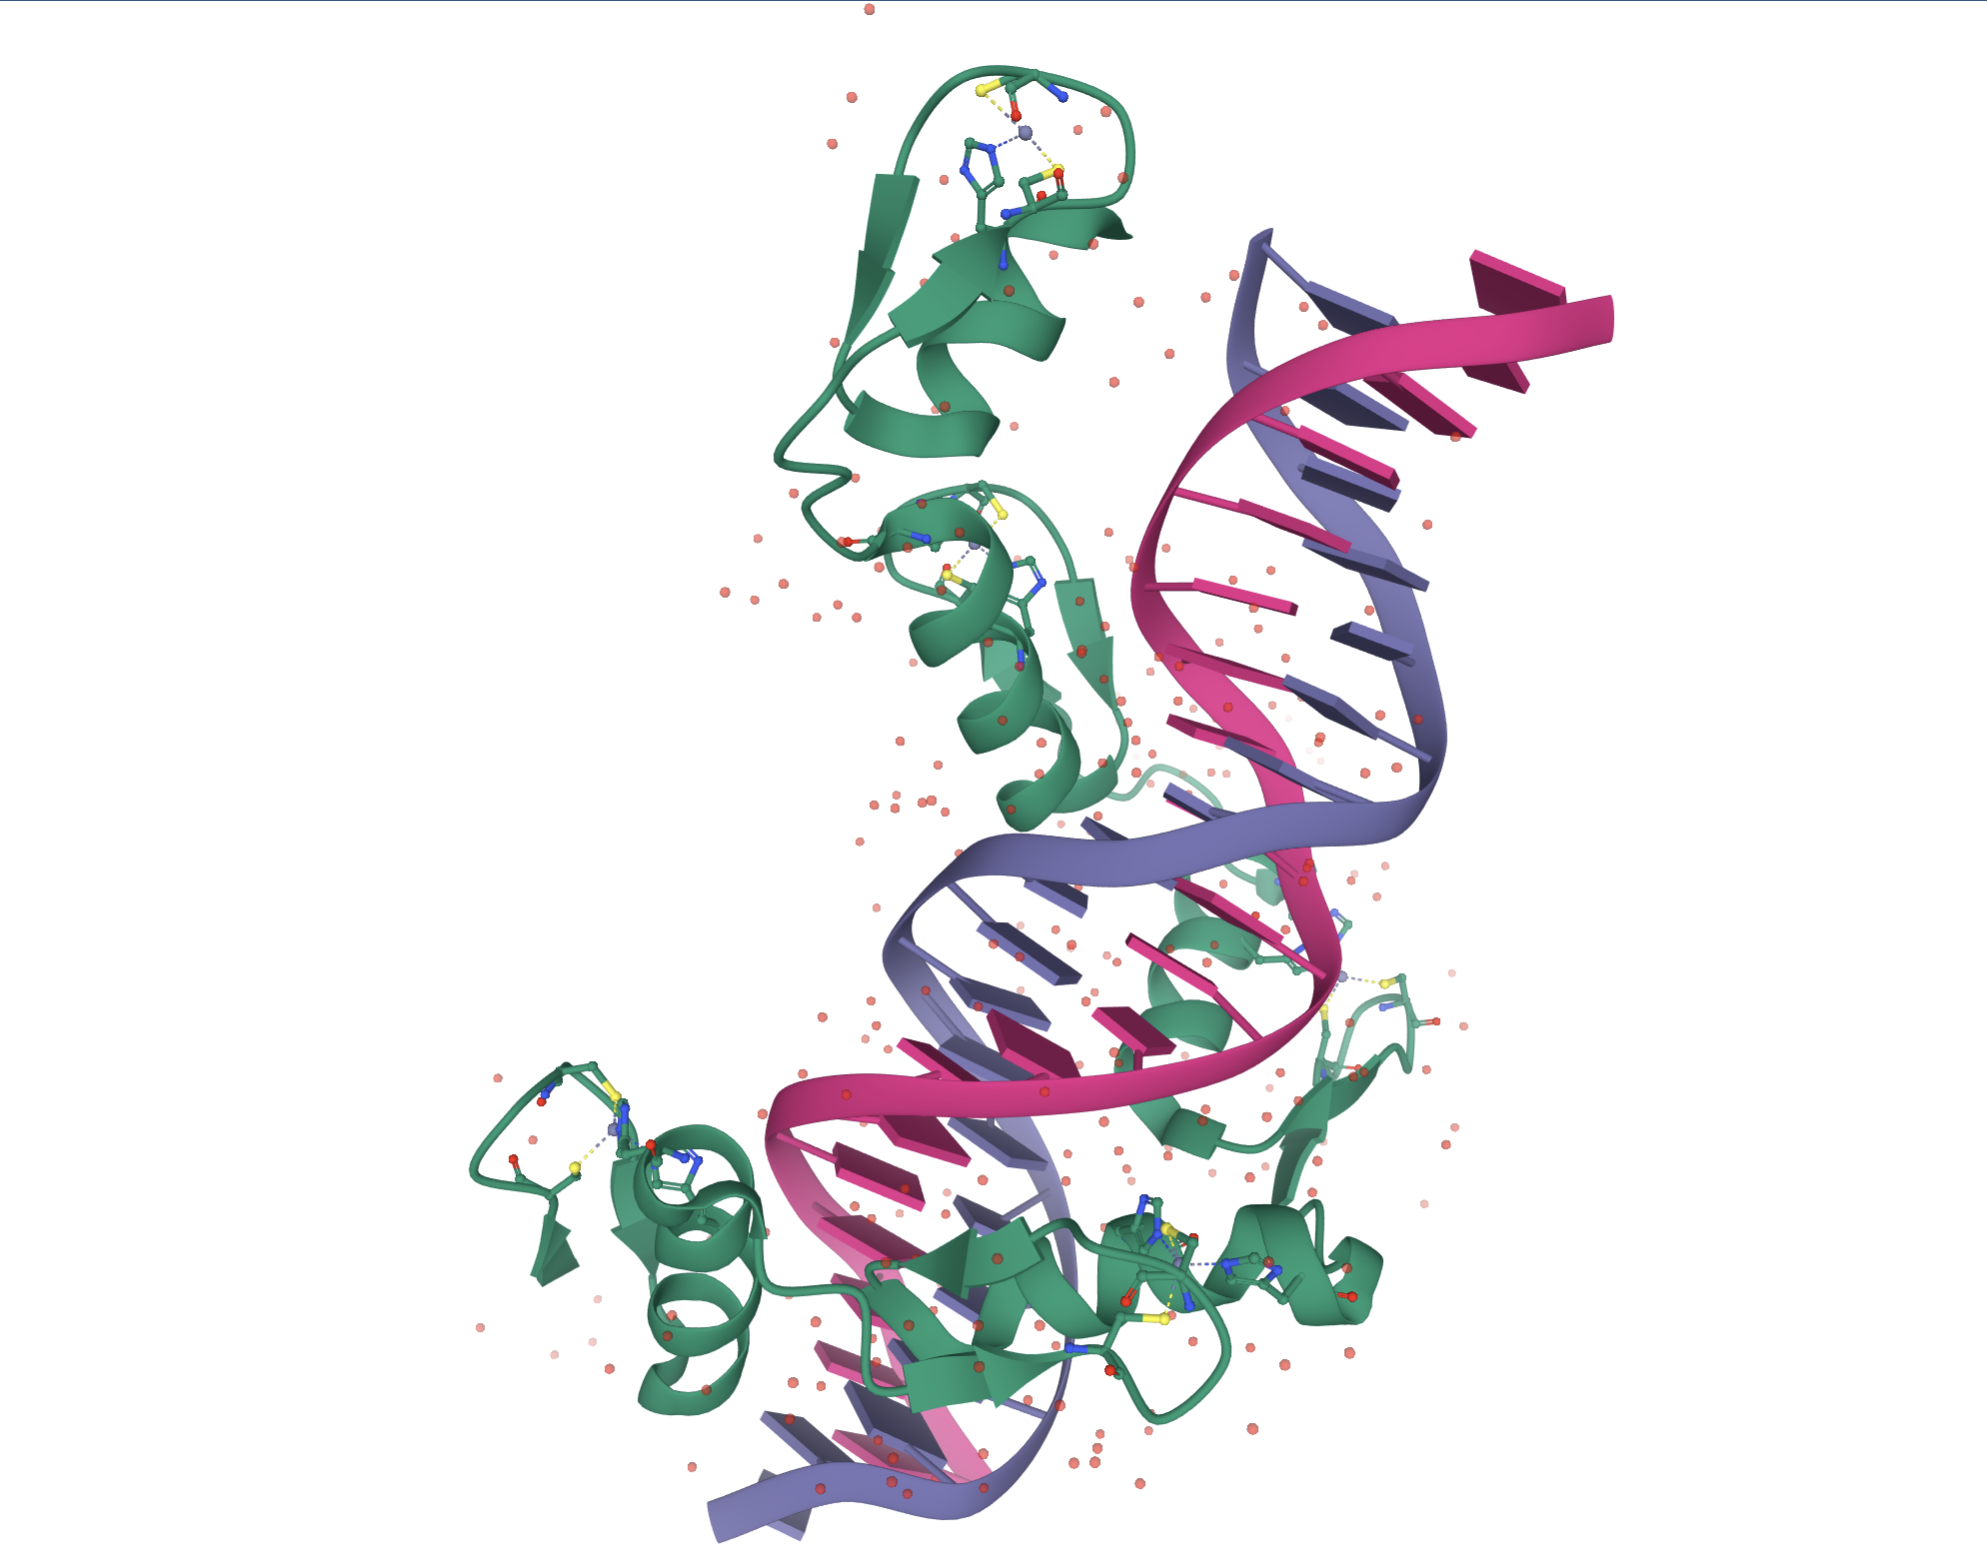
\includegraphics[width=\textwidth]{figures/ctcf_dna.png}
	\caption[A human transcription factor (CTCF) binding its DNA target sequence.]{\textbf{A human transcription factor (CTCF) binding its DNA target sequence.}}
	\label{fig:ctcf_dna}
\end{figure}
% ---- Discovering Transcription Factor Binding Site motifs
\section{Discovering Transcription Factor Binding Site motifs}
Several experimental assays have been developed to determine the binding site sequences of TFs in living cells or organisms (\emph{in vivo}), or in test-tubes using synthetic or purified components (\emph{in vitro}) \citep{jolma2011methods}. Early methods, like electrophoretic mobility shift assay (EMSA) \citep{garner1981gel} or footprinting \citep{hampshire2007footprinting},  generally analyze a relatively small number of target sequences to find TFBS. As a result, they return small datasets of bound sequences. \emph{In vitro} and \emph{in vivo} high-throughput protocols such as PBM, SELEX or ChIP methods \citep{berger2006compact,jolma2010multiplexed,collas2008chop}, facilitated the analysis of most target sites for factors of interest. As a result, large datasets of bound sequences have been generated, presenting an unprecedented opportunity to study and determine the TF binding landscapes. Experimental assays can recover the sequences bound by TFs along with their relative or absolute binding affinity. However, such datasets can incorrectly report unbound sequences as binding sites. In addition, the assays usually capture extra nucleotides in target sites, reducing data resolution and making manual analysis challenging. Motif discovery algorithms provide a computational framework to analyze these large datasets generated by experimental assays, discovering the sequences potentially bound by TFs and predicting their affinities \citep{pavesi2004silico,tompa2005assessing,d2006does,das2007survey,zambelli2013motif,tognon2023survey}. Given a sequence dataset, these algorithms typically recover sets of short and similar sequence elements. The prioritized sequence elements are later used to construct a motif model, summarizing the diverse binding site configurations observed among the prioritized sequences, and encoding their recurrent patterns and similarities (\textbf{Fig.\ref{fig:md} (A)}). Several methods and models have been proposed to discover and represent TFBS motifs. Position weight matrices (PWMs) \citep{stormo2000dna} are the most popular models. PWMs are simple yet powerful and interpretable models, encoding the probability of observing a given nucleotide in each TFBS position. However, PWMs have some limitations, like the assumption of independence among the binding site positions. Therefore, several alternative motif models have been proposed \citep{siddharthan2010dinucleotide,gorkin2012integration,he2021survey} , as described below. The derived motif models can be employed in many downstream analyses, like searching potential binding site occurrences in regulatory genomic sequences, predicting the sets of genes regulated by the investigated TFs or assessing how genetic variants could affect their binding landscape.
% -- Experimental methods to discover Transcription Factor Binding Sites
\begin{figure}
	\centering
	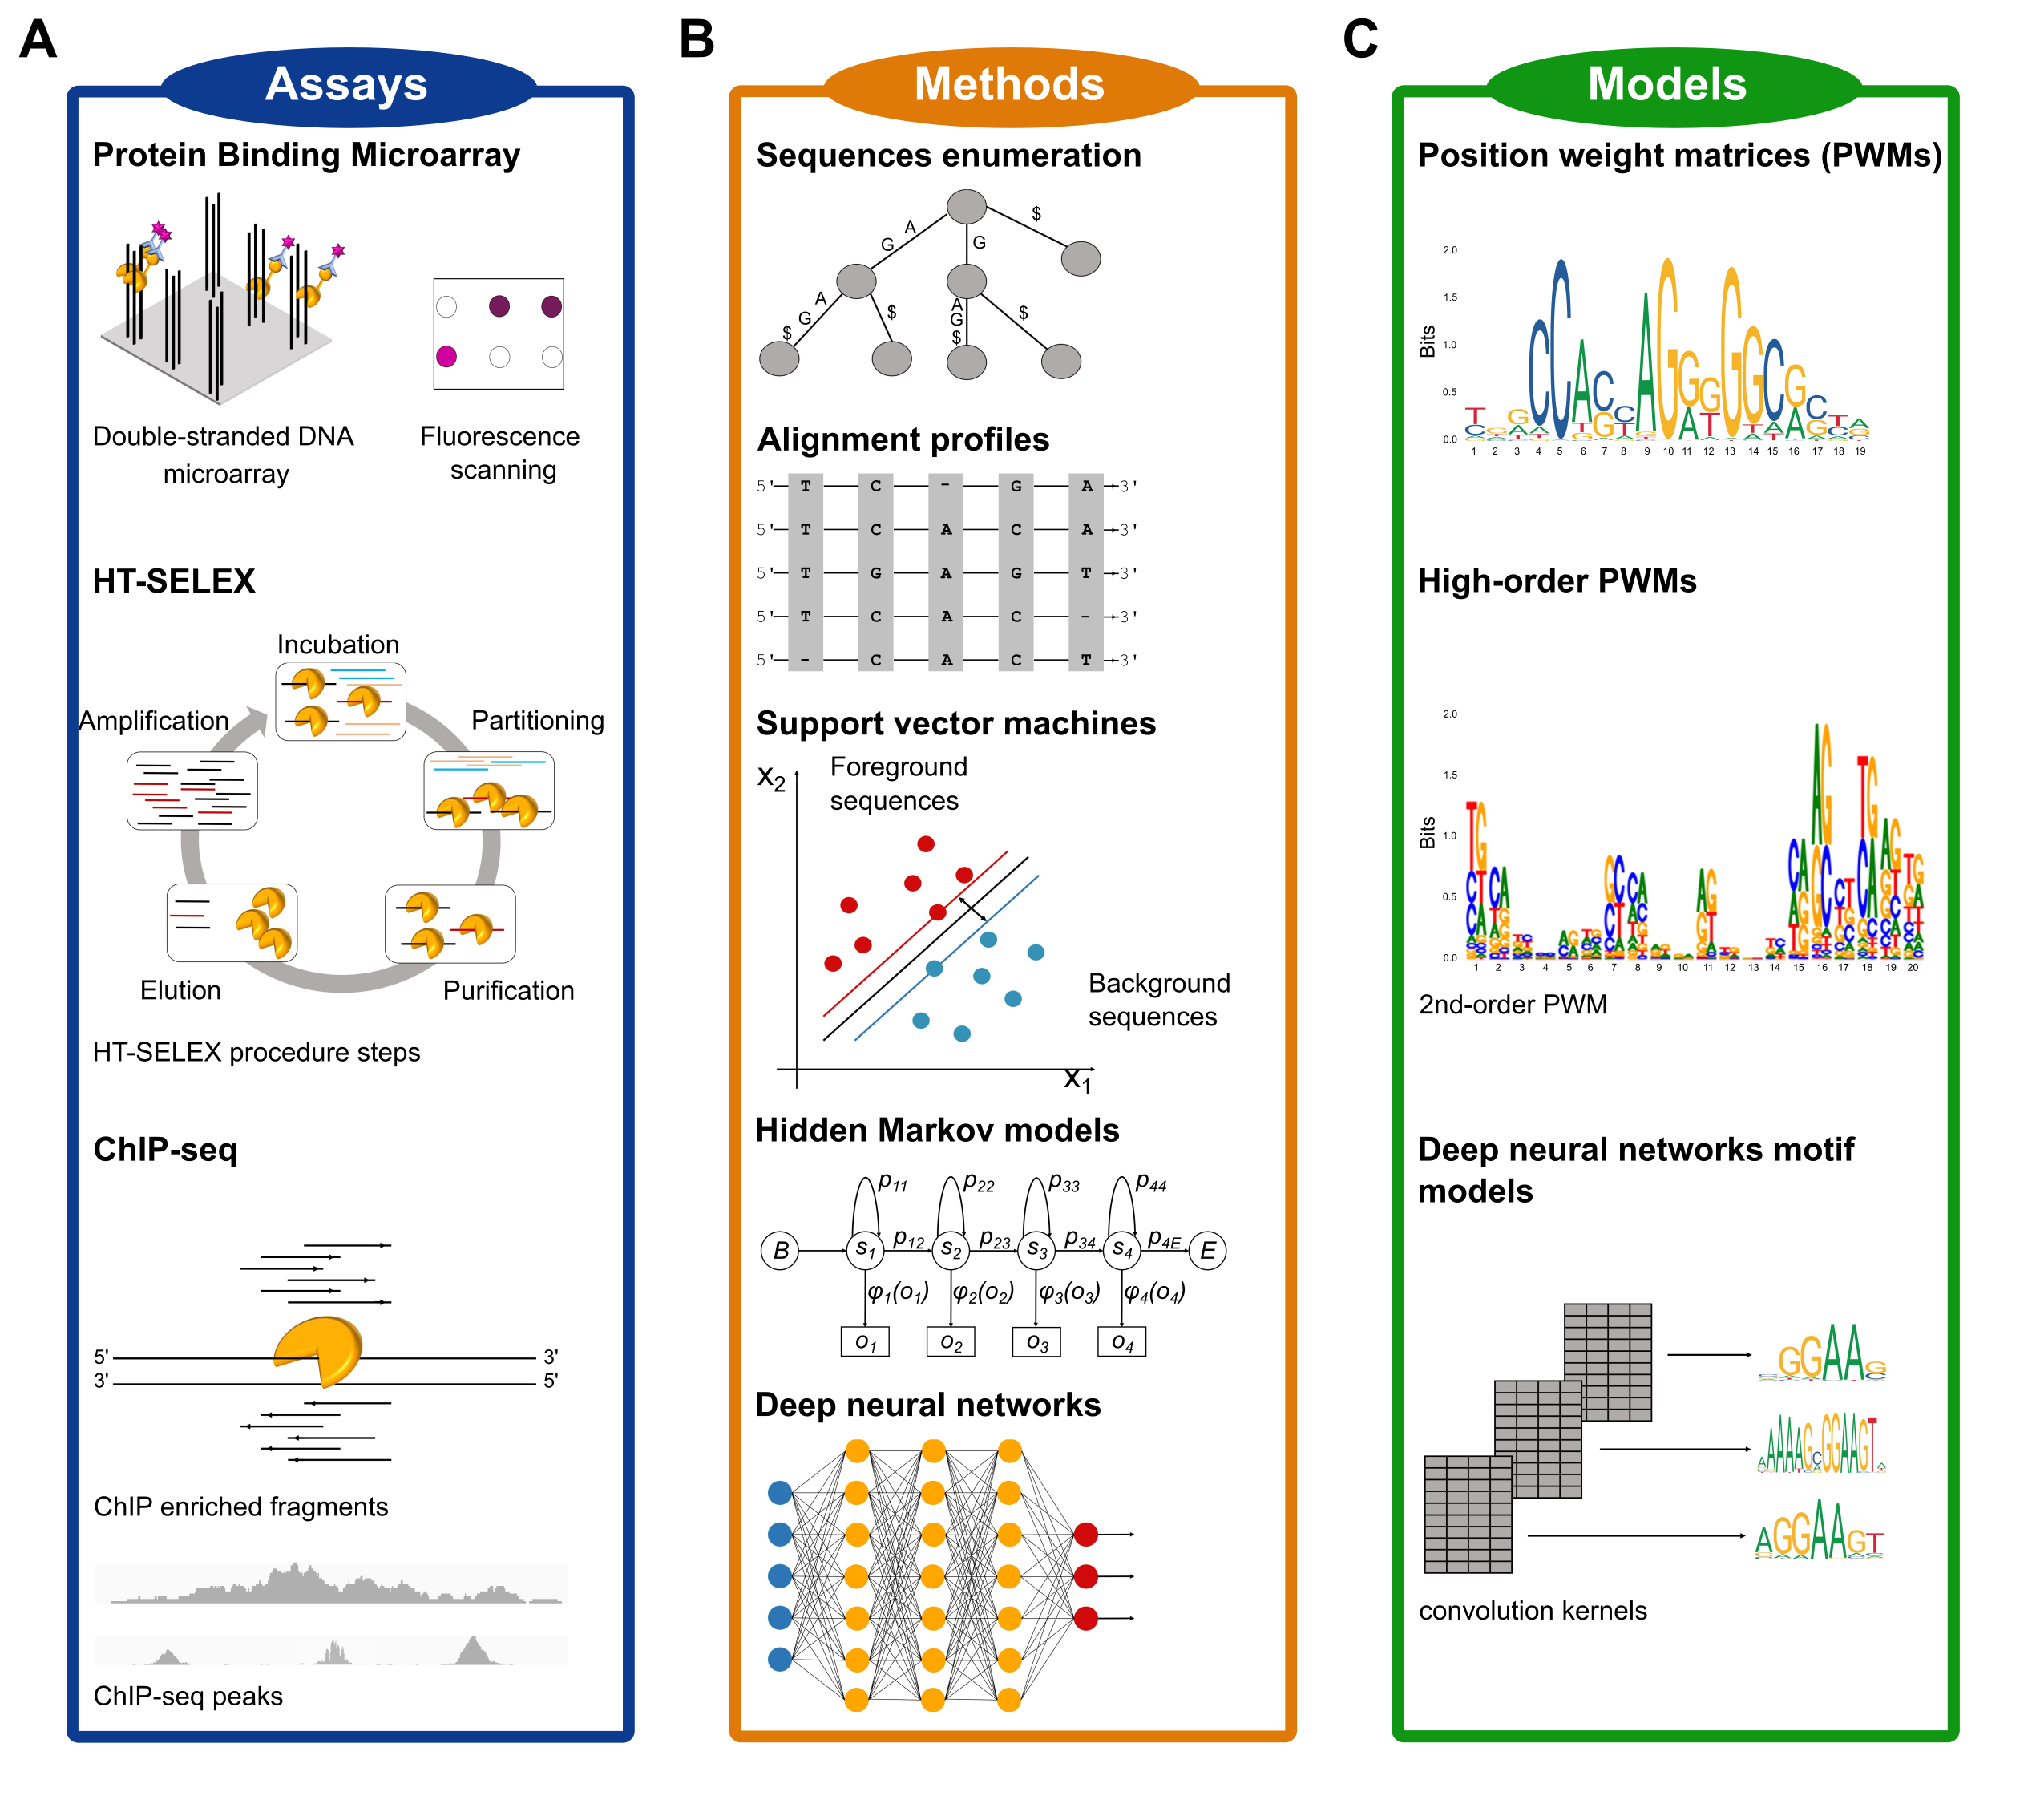
\includegraphics[width=\textwidth]{figures/md.png}
	\caption[Experimental and computational methods to discover TFBS and popular models to represent binding site motifs.]{\textbf{Experimental and computational methods to discover TFBS and popular models to represent binding site motifs.} Protein binding microarray (PBM), HT-SELEX and ChIP-seq have become the most popular assays to determine TF binding preferences and identify their target sites (TFBS) in recent years. Computational motif discovery methods can be grouped into five classes, based on the algorithms employed to discover TFBS: enumerative, alignment-based, probabilistic graphical model-based, SVM-based and DNN-based methods. TFBS sequences prioritized by motif discovery algorithms are encoded in computational models representing the binding preferences of the investigated TFs.}
	\label{fig:md}
\end{figure}
\subsection{Experimental methods to discover Transcription Factor Binding Sites}
During the last decades, several techniques have been introduced to experimentally identify and assess TF binding sites and binding preferences \citep{jolma2011methods} (\textbf{Fig.\ref{fig:md}} and \textbf{Table \ref{table:assays}}). Early studies on TF binding focused their analysis on gene promoters \citep{stormo2000dna} and employed in vitro methods, such as Electro-Mobility Shift Assay (EMSA) \citep{garner1981gel} or DNase footprinting \citep{galas1978dnaase}. EMSA exploits non-denatured polyacrylamide gel properties to separate bound and unbound DNA sequences. DNase footprinting combines EMSA with DNase I cleavage, identifying uncut regions (footprints) due to the protection of the bound TF. Generally, these assays produce datasets of a few hundred of bound sequences, exploring a limited spectrum of TFs binding landscape. Moreover, EMSA and DNase footprinting may be subject to technical constraints that could lead to inaccuracies in the reported sequences and binding preferences \citep{jolma2011methods}.  The introduction of NGS technologies revolutionized the study of TFBS identification by encouraging researchers to develop methods that exploit the power of massively parallel sequencing (\textbf{Fig.\ref{fig:md}}). These methods have two major advantages: (i) they do not require any prior knowledge on the binding site sequence \citep{jolma2011methods, zia2012towards} and (ii) produce datasets of thousands of bound sequences allowing a better characterization of TF binding preferences \citep{stormo2010determining}. Protein binding microarrays (PBMs) \citep{berger2006compact,berger2009universal} recover short TFBS sequences ($\sim$10 bp) and measure TF binding preferences in vitro. In PBMs, a tagged TF is released on a glass slide containing thousands of spots filled with short, immobilized DNA sequences. The tagged TFs are then incubated with fluorescent antibodies against the tag and subsequently washed to remove weakly bound factors. The fluorescence and DNA sequence enrichment are then used to quantify the TF–DNA binding strength and capture the bound sequences. Generally, the recovered sequences do not contain nucleotides flanking the investigated binding sites, producing high-resolution datasets. However, since the number of possible sequences grows as a function of the target length, PBMs can assess only a limited number of target sequences \citep{jolma2011methods, zia2012towards}. PBM analysis is usually constrained to binding sites $\sim$10–12 bp long. HT-SELEX \citep{jolma2011methods,jolma2010multiplexed} is a widely used \emph{in vitro} method, coupling SELEX with high-throughput sequencing. A TF is released on a pool of randomized DNA sequences to allow the factor to select its target sites. The resulting TF–DNA complexes are separated from unbound sequences using affinity capture, and subsequently amplified through polymerase chain reaction (PCR) and sequenced. The resulting DNA library is enriched in binding sites for the studied TF and is used as the starting pool for another SELEX run \citep{jolma2011methods,jolma2010multiplexed}. SELEX does not require any prior knowledge on the target sites of the investigated factor \citep{jolma2013dna}. Since SELEX reaction is typically performed in liquid phase and consequently does not suffer from physical constraints, the sequence space covered by HT-SELEX is often larger than that of PBMs. Moreover, by coupling sequencing with DNA barcode indexing, HT-SELEX allows to analyze hundreds of TFs in parallel. HT-SELEX produces datasets of thousands of high-resolution bound sequences, which include only a few nucleotides flanking the binding sites. However, since the starting DNA library is constituted by randomized sequences, HT-SELEX cannot recover the genomic binding locations for the investigated factor. The introduction of chromatin immunoprecipitation (ChIP) technologies \citep{collas2008chop}. radically changed the study of TFBS binding, enabling the genome-wide identification of regions bound by TFs in vivo. In ChIP, the TF–DNA complexes are cross-linked using formaldehyde. The DNA is then fragmented in $\sim$100–1000 bp long fragments and subsequently immunoprecipitated with antibodies specific for the investigated TF. To recover the bound sequences, the cross-links are reverted. Then, the resulting fragments are amplified through microarray hybridization (ChIP-on-Chip \citep{collas2008chop,pillai2015chip}) or sequencing (ChIP-seq \citep{johnson2007genome,mardis2007chip}). To locate the binding regions, the recovered DNA fragments are mapped onto the genome. After ChIP-seq reads mapping, peak calling algorithms \citep{thomas2017features,guo2012high,zhang2008model} are employed to predict the genomic binding locations for the investigated factor. Peak calling algorithms identify the genomic regions showing greater enrichment in mapped DNA probes with respect to a control experiment and mark those regions as binding locations, or peaks  \citep{pepke2009computation}. ChIP methods produce large datasets of thousands of genomic regions, whose length ranges from few hundreds to thousands of nucleotides, from which we can identify the likely TFBS for the investigated factor. Although ChIP technologies, and particularly ChIP-seq, are currently considered the current ‘golden standard’, they have some limitations. (i) ChIP can detect indirect binding, identifying other TFBS not belonging to the investigated factor \citep{worsley2014non}. (ii) ChIP-seq peaks may be false positives, recovered because of poor antibody quality \citep{pickrell2011false}. (iii) ChIP-seq returns low-resolution datasets, whose sequences include several nucleotides flanking the target TFBS. ChIP-exo  \citep{rhee2011comprehensive} addresses the latter issue, employing a lambda exonuclease to trim ChIP sequences, removing some of the nucleotides flanking the target sites. Alternatively, since most TFs bind their target sequences in open chromatin regions, experimental assays targeting open chromatin like ATAC-seq or DNase-seq \citep{buenrostro2013transposition,john2011chromatin} can be employed to recover in vivo genomic locations likely to contain TFBS. ATAC-seq and DNase-seq are generally employed when the factors binding the target regions are not known.In summary, the current high-throughput in vivo and in vitro assays generate datasets of thousands of sequences potentially containing several possible binding configurations of TFBS, thereby enabling better characterizations of TFs binding landscapes.
\begin{longtable}{|p{2.4cm}|p{4cm}|p{1.75cm}|p{1.5cm}|p{1cm}|p{2.3cm}|p{2cm}|}
	%\centering
	%\begin{tabular}{|p{2.4cm}|p{4cm}|p{1.75cm}|p{1.5cm}|p{1cm}|p{2.3cm}|p{2cm}|}
		\hline
		\textbf{Experimental assay}& \textbf{Description}&\textbf{Output}&\textbf{\emph{De novo} motif discovery capability}& \textbf{Type}& \textbf{Identification of genomic binding locations}& \textbf{Throughput} \\
		\hline
		Competition EMSA& Bound DNA sequences are identified by observing changes in the electrophoretic migration of DNA sequences through non-denatured polyacrylamide gel& Bound DNA sequences& No. Used to validate known binding sites& \emph{in vitro}& No& Low\\  
		\hline
		DNase footprinting& Pools of DNA sequences are incubated with the TF of interest; then, the DNA is degraded using DNase I. The unbound fragments are cut in all positions, while the bound DNA is protected by the TF& Bound DNA sequences.& No. Used to validate known binding sites.& \emph{in vitro}& No& Low\\
		\hline
		Protein Binding Microarrays& Arrays of $\sim$40 000 spots with short, immobilized DNA sequences are incubated with a tagged TF, and then washed to remove weakly bound proteins. The bound sequences are identified through fluorescence-based detection & Continuous values describing fluorescence intensity on each array spot & Yes. Limited to short motifs ($\sim$12bp)& \emph{in vitro}& No& High\\
		\hline
		HT-SELEX& The TF is added to a pool of randomized DNA fragments. The bound sequences are selected and constitute the starting pool for the next experimental round. The procedure is repeated for several rounds. Sequencing is employed to recover the sequence of the bound DNA fragments & DNA sequences& Yes& \emph{in vitro}& No& High\\
		\hline
		ChIP-based technologies& TF–DNA complexes are cross-linked with formaldehyde and immunoprecipitated employing TF-specific antibodies. The bound sequences are then prioritized employing qPCR microarrays (ChIP-on-Chip) or through sequencing (ChIP-seq). ChIP-exo integrates exonuclease treatment to enhance sequence resolution & Genomic binding location coordinates& Yes. Limited by the inability to distinguish direct and indirect binding& \emph{in vivo}& Yes& Low\\
		\hline
	%\end{tabular}
	\caption[\emph{In vivo} and \emph{in vitro} experimental assays to identify and validate transcription factor binding sites.]{Generally, EMSA and DNase footprinting are used to validate known TFBS, while currently PBMs, HT-SELEX and ChIP-based methods are preferred to discover novel binding sites. ChIP-based assays are the only methods that recover the TF genomic binding locations. The throughput column refers to the number of samples that can be processed in parallel by each method (high: hundreds of samples; low:a few samples).}
	\label{table:assays}
\end{longtable}

% -- Computational methods to discover Transcription Factor Binding Sites
\subsection{Computational methods and models to discover and represent Transcription Factor Binding Sites}
The TFBS motif discovery problem can be formalized as follows. Given a set of positive DNA sequences $S$, obtained from an experimental assay targeting a certain TF, and a set of negative sequences $B$ the goal is to find one or more recurrent, short and similar subsequences in $S$ that maximize the discriminatory power between $S$ and $B$. Such subsequences are called patterns or motifs and are likely bound by the investigated TF.  The negative set $B$ can contain randomly generated or selected genomic sequences, with similar nucleotide content and length of those in $S$. The retrieved patterns are used to construct and train a computational model $M$ (motif model), representing the discovered motif. These models can then be used to identify new potential binding sites, given a new set of sequences, and to predict the strength of the TF–DNA binding. Motif discovery can be considered a classification or a regression problem, depending on the type of data used to train $M$ \citep{tognon2023survey}.  The datasets derived by experimental assays like ChIP-seq or HT-SELEX provide hundreds or thousands of sequences containing binding sites. In this setting, motif discovery becomes a classification problem. In fact, the goal is to discriminate between bound and unbound sites in the input sequences and train the motif model with the identified binding sites. The datasets produced by other experimental technologies like PBMs provide the relative binding strength for large sets of sequences of equal length. Therefore, rather than discriminating between bound and unbound sequences, in this setting $M$ learns the relative binding affinities associated to each target site in the input dataset, transforming motif discovery into a regression problem. In both settings, the final goal is to derive a computational model $M$, describing the recovered TFBS and capable of predicting new binding events, along with their affinity, in sequences not used during model training. Motif discovery algorithms can be classified in enumerative, alignment-based, probabilistic graphical models, support vector machine (SVM)-based and deep neural network-based methods (\textbf{Fig.\ref{fig:md}}).Other approaches to discover TFBS motifs in genomic sequences use phylogenetic footprinting \citep{mccue2001phylogenetic,blanchette2002discovery}. The core principle of phylogenetic footprinting is that functional elements, such as TFBS, are more likely to be conserved across evolutionarily related species, while non-functional elements are more susceptible to mutations. Although phylogenetic footprinting was one of the first techniques proposed for identifying TFBS, it is still widely used to examine TFBS conservation across different organisms \citep{balazadeh2011ors1, xu2012cis,katara2012phylogenetic}. In a recent study \citep{glenwinkel2014targetortho},  the authors proposed a novel method that utilizes phylogenetic footprinting to discover TFBS. Before describing the algorithms, we briefly review the models to describe TFBS motifs.The most common models to represent TFBS are consensus sequences  \citep{day1992critical}, PWMs \citep{stormo2000dna,stormo2013modeling},  high-order PWMs \citep{siddharthan2010dinucleotide,korhonen2017fast},, SVM-based  \citep{gorkin2012integration} and deep neural network-based  \citep{he2021survey} models. Consensus sequences summarize the discovered TFBS by denoting the most frequently observed nucleotide at each motif position in a prioritized sequence set. Although TFBS have conserved positions not tolerant to mutations \citep{li2015human}, other binding site locations admit alternative nucleotides. Degenerate consensus accommodates ambiguous motif positions employing IUPAC symbols. However, consensus sequences cannot encode the contribution to TF–DNA binding of each nucleotide at each motif position. PWMs address this limitation, providing an additive model with the contribution of each motif position to the binding site. PWMs construct an ungapped alignment between motif candidate sequences and count the frequency of each nucleotide at each position. The statistical significance of PWMs is often measured employing relative entropy (RE) \citep{stormo1998information}. RE quantifies the difference between computed nucleotide frequencies and those obtained from aligning random sequences. PWMs are visualized as logos \citep{schneider1990sequence}, where the height of each nucleotide is proportional to its RE. Despite their wide success, PWMs still assume independence between motif positions.Probabilistic graphical models address this limitation by modeling dependency between motif nucleotides. These models include high-order PWMs like dinucleotide weight matrices (DWMs), Bayesian networks (BNs), Markov models (MMs) or hidden Markov models (HMMs) \citep{siddharthan2010dinucleotide, korhonen2017fast, barash2003modeling, siebert2016bayesian}. DWMs and high-order PWMs are often visualized as logos with $q$-mers replacing the single nucleotides, where $q$ is the dependency order between neighboring nucleotides. Importantly, probabilistic graphical models can account for variable spacing between half-sites of two box motifs. However, the number of model’s parameters and its complexity grow exponentially with $q$, often resulting in the model overfitting the input dataset. SVM-based models train a SVM kernel learning the binding site structure from the input sequence dataset. TFBS are represented by either a list of $k$-mers with associated weights or support vectors used to discriminate between bound and unbound sequences, depending on the employed kernel \citep{boeva2016analysis}. In the former case, the weights reflect the $k$-mer contribution to the motif sequence. SVM-based models can account for variable spacing between the half-sites of two box motifs, like probabilistic graphical models. Importantly, $k$-mers indirectly capture $k$-th order dependencies between neighboring nucleotides. However, simple SVM-based models are limited to consider short $k$ ($\sim$10 bp) and cannot represent longer motifs. Gapped $k$-mers \citep{ghandi2014robust} addressed this limitation, handling longer TFBS and sequence degeneration in non-informative motif positions. To visualize the discovered motifs, SVM-based models are often reduced to PWMs computed aligning the informative $k$-mers. Deep neural network (DNN)-based models integrate the diverse, complex and hierarchical patterns governing TF–DNA binding events in input nucleotide sequences. Although DNN-based models are accurate and powerful, their ‘black box’ nature is a major limitation \citep{park2020enhancing}. Many frameworks visualize the discovered motifs as PWMs, computed aligning the sequences activating the convolutional kernels of the DNN \citep{koo2020deep}. However, DNNs often learn distributed representations where multiple neurons cooperate to describe single patterns. Therefore, motifs learned by single kernels and the resulting PWMs are often redundant with each other. DeepLIFT \citep{shrikumar2017learning} proposed a method to assign importance scores to the kernels. Comparing the activation of each neuron to a reference value, DeepLIFT selects which kernels contribute most to the TFBS definition, reducing motif redundancy. TF-MoDISco \citep{avsec2021base} extended this idea by clustering and aggregating the discovered motifs, using the importance scores assigned to the kernels. However, computing interpretable models without losing some information learned by the DNN is still an open challenge.
\subsubsection{Enumerative methods}
Enumerative motif discovery algorithms (\textbf{Fig.\ref{fig:md}}) assume that motifs are overrepresented patterns in the input dataset $S$, with respect to a set of background genomic sequences $B$. Enumerative algorithms may assume that the motif length $|M|$ is known a priori. Given $|M| = k$, the general idea is to collect the approximate occurrences of all potential $4^{k}$ $k$-mers in the sequences of $S$ and assess if the difference between the number of matches found in $S$ and $B$ or the expected number of matches from a background model is statistically significant. Then, a PWM is obtained building an ungapped alignment from the statistically significant $k$-mers. Searching the approximate occurrences of all $4^{k}$ $k$-mers quickly becomes impractical, even for small $k$. Early proposals introduced the usage of heuristics to reduce the search space, for example, searching only patterns occurring at least once in each sequence $s \in S$ \citep{li1999finding} or restricting mismatching locations to specific motif positions \citep{califano2000splash}. However, mismatches can occur at any motif position. Weeder \citep{pavesi2001algorithm, pavesi2004weeder} and SMILE \citep{marsan2000algorithms} proposed using suffix trees (STs) \citep{weiner1973linear} to efficiently explore the entire motif search space. They leverage the indexing capabilities of STs to perform approximate pattern matching, without restrictions on mismatching positions. This enabled achieving high accuracy in motif discovery, while reducing computational costs. To determine the statistical significance of motif candidates, SMILE and Weeder compare the motifs frequencies in $S$ with those in a set of random genomic sequences or the promoters of the same organism, respectively. However, these approaches can be computationally intensive and are not scalable on the large datasets generated by PBMs, HT-SELEX or ChIP assays \citep{liu2018algorithmic}. Therefore, more efficient approaches specifically tailored to work on large datasets were proposed. MDscan \citep{liu2002algorithm} and Amadeus \citep{linhart2008transcription} use word enumeration to discover motif candidates in sequence datasets. MDscan employs ChIP peaks shape to identify non-redundant patterns abundant in the most enriched sequences and uses a third-order Markov background model to assess motif statistical significance. Amadeus evaluates all $k$-mers in $S$ and groups similar patterns in list. Each list is grouped into motifs, statistically evaluated using a hypergeometric test. However, word enumeration can be still computationally demanding. To address this challenge, DREME  \citep{bailey2011dreme} proposed using regular expressions to count approximate frequencies of motifs in $S$ and $B$. To evaluate the motifs’ statistical significance, DREME employs Fisher’s exact test, comparing the number of sequences in $S$ and $B$ in which the motifs occur. However, regular expressions can be computationally expensive when analyzing large $S$, and may detect false positives or miss motifs. Trawler, HOMER and STREME \citep{ettwiller2007trawler,heinz2010simple,bailey2021streme} reintroduced STs, proposing different optimizations to make the methods scalable on large datasets. Trawler and HOMER optimized the statistical assessment step using $z$-scores derived from the normal approximation to the binomial distribution and the hypergeometric distribution, respectively. Instead of improving the statistical assessment, STREME reduces the motif search space by first identifying overrepresented seed words of different lengths on the ST. Then, STREME counts the number of approximate matches of the most significant words on the ST. By identifying seeds of different lengths, STREME discover motifs of different lengths in one single tree visit.
\subsubsection{Alignment-based methods}
Alignment-based motif discovery algorithms compute alignment profiles to describe motifs binding preferences (\textbf{Fig.\ref{fig:md}}), avoiding exhaustive $k$-mer enumeration. This approach involves constructing an alignment by selecting motif candidate sequences from the input dataset $S$ and evaluating the resulting profile using various measures, like nucleotide conservation, information content or profile statistical significance. Motif statistical significance is determined by computing the probability of obtaining the same alignment from either a background dataset $B$ or random sequences. Alignment-based motif discovery algorithms typically assume that the motif length $|M|$is known a priori. For alignment-based algorithms, motif discovery can be formalized as a combinatorial problem. Given $|M| = k$ the goal is to find the best alignment profile by combining $k$-mers from $S$ according to a scoring criterion. The best alignments are then used to generate the corresponding PWMs. Most alignment-based algorithms assume that each sequence in $S$ contains zero or one binding site. Therefore, there exist $(\sum_{s \in S}{|s| - |M| + 1})^{|S|}$ possible profiles, built by combining $k$-mers in all possible ways. Since enumerating all possible solutions is computationally impractical even for small datasets, alignment-based algorithms employ heuristics, such as greedy \citep{hertz1999identifying}, expectation-maximization (EM) \citep{bailey1994fitting}, stochastic (e.g. Gibbs sampling) \citep{lawrence1993detecting}, or genetic algorithms \citep{lee2018comprehensive}.  CONSENSUS \citep{hertz1999identifying} proposed a greedy approach to construct alignment profiles incrementally. It solves the problem initially on two sequences and progressively solves it by adding the remaining sequences $s \in S$ one by one. CONSENSUS stores the best partial alignments hoping to find the highest-scoring profiles. However, if motifs are not conserved, CONSENSUS may potentially discard the highest-scoring solutions. The MEME algorithm \citep{bailey1994fitting,bailey1995value,bailey2006meme} proposed a different strategy based on EM. It iteratively refines an initial profile by substituting some $k$-mers in the profile, with others more likely to produce better solutions. MEME evaluates the fit of each $k$-mer in $s \in S$ to the current profile, rather than a background model. MEME identifies motifs occurring more than once in each sequence and computes their statistical significance, and the method does not rely on TFBS conservation. However, the algorithm may converge prematurely to local maxima and convergence heavily depends on the algorithm starting conditions. In contrast to MEME, Gibbs sampling \citep{lawrence1990expectation} employs a stochastic approach to add $k$-mers to the alignment instead of a deterministic one based on the profile fit. Gibbs sampling replaces $k$-mers in the profile with others selected with probability proportional to its likelihood score. The algorithm’s stochastic nature reduces its likelihood to converge to local maxima, but it may require multiple runs to achieve reliable results. However, several methods using Gibbs sampling and its extensions have been proposed \citep{neuwald1995gibbs, hughes2000computational, workman1999ann, liu2000bioprospector, thijs2001higher, frith2004finding}. Genetic algorithms are an alternative approach overcoming the limitations of EM and stochastic methods. GADEM \citep{li2009gadem} combined EM local search with genetic algorithms to refine profiles, avoid convergence to local maxima and overcome Gibbs sampling stochastic nature. However, due to their computational complexity, genetic algorithms are computationally demanding when analyzing thousands of sequences. Using alignment profiles, the solution space grows exponentially with the size of $S$ and even with employing heuristics analyzing thousands of sequences is computationally impractical \citep{zambelli2013motif}. MEME-ChIP \citep{machanick2011meme} and STEME \citep{reid2011steme} improved the MEME algorithm to analyze ChIP datasets. While MEME-ChIP focuses the analysis on a random subset of sequences, STEME speeds up EM steps indexing the sequences in a suffix tree. However, using random subsets of $S$ may cause missing critical motif instances and constructing ST from thousands of sequences may be computationally demanding. ChIPMunk \citep{kulakovskiy2010deep} proposed a greedy profile optimization like EM developed to discover motifs in large ChIP-seq datasets, while accounting for ChIP peaks shape. XXmotif \citep{hartmann2013p} and ProSampler \citep{li2019prosampler} proposed methods combining enumerative motif discovery with iterative and stochastic profile refinement, respectively.

\subsubsection{Probabilistic graphical model-based algorithms}
The inclusion of dependencies between nucleotides in TFBS has been subject of debate \citep{tomovic2007position, morris2011jury, zhao2011quantitative}.  Some studies have shown that dependencies exist between neighboring and non-neighboring nucleotides in TFBS \citep{slattery2014absence, rohs2010origins}. Enumerative and alignment-based algorithms represent motifs as PWMs, which do not account for dependencies between the binding site positions. PWMs can be extended to account for the frequency of di- or trinucleotides (high-order PWMs), like DWMs \citep{siddharthan2010dinucleotide}. Dimont \citep{grau2013general} and diChIPMunk \citep{kulakovskiy2013binding} proposed extensions to alignment-based methods to discover and represent motifs as DWMs. However, these methods capture dependencies only between neighboring nucleotides. Probabilistic graphical models (\textbf{Fig.\ref{fig:md}}) such as BNs, MMs or HMMs provide powerful frameworks for capturing dependencies between TFBS nucleotides. In \citep{barash2003modeling} the authors proposed using BNs trained via EM to model TFBS. The proposed approach captures dependencies between neighboring and non-neighboring positions but assumes the same order of dependence throughout the entire motif. Similarly, in \citep{ben2005identification}, the authors introduced VOBN models. VOBNs use BNs accounting for variable orders of dependencies between positions. However, training BNs is not computationally scalable when analyzing thousands of sequences and these models are prone to overfitting when trained on hundreds of sequences. MMs and HMMs provide more efficient and scalable frameworks than BNs to include dependencies between motif positions. Therefore, researchers focused on developing algorithms using these models to learn dependencies in large sequence datasets produced by NGS assays. TFFMs \citep{mathelier2013next}  and Discrover \citep{maaskola2014binding} proposed HMM-based models learning the dinucleotide dependencies between neighboring motif positions in large sequence datasets. In addition, TFFMs learn the properties of the sequences flanking the TFBS. MMs can be extended to capture different orders of dependencies between neighboring nucleotides, as demonstrated in \citep{eggeling2014value}, where the authors proposed a method to discover CTCF citep{bell1999protein} motifs using variable-order MMs. Similarly, MMs can also be extended to capture dependencies between non-neighboring nucleotides as proposed in Slim \citep{keilwagen2015varying}. However, MMs and HMMs typically only capture low-order dependencies. BaMMotif  \citep{siebert2016bayesian, ge2021bayesian} proposed a motif discovery algorithm employing a Bayesian approach to efficiently train Markov models up to fifth-order dependencies on thousands of sequences.
\subsubsection{SVM-based methods}
SVMs \citep{boser1992training} have been successfully applied to different problems in computational biology  \citep{ben2008support}, including TFBS motif discovery (\textbf{Fig.\ref{fig:md}}).  This is achieved by decomposing bound (foreground dataset $S$) and unbound sequences (background dataset $B$) in $k$-mers and using their frequencies as features to train a sequence similarity kernel \citep{ben2008support}.  Generally, to each $k$-mer is assigned a weight proportional to its contribution to the definition of the positive or negative training sets, or to its likelihood of being a motif candidate. While earlier methods \citep{leslie2001spectrum,  eskin2002mismatch, kuang2005profile} were designed for protein sequence homology, recent SVM-based algorithms have been developed to discover TFBS motifs. Furthermore, SVMs can efficiently analyze datasets of thousands of sequences. Kmer-SVM \citep{lee2011discriminative, fletez2013kmer} proposed a method to discover TFBS motifs in sequence datasets, using the spectrum kernel \citep{leslie2001spectrum} Kmer-SVM counts the exact matches for all contiguous $k$-mers in $S$ and $B$, building the $k$-mers feature space. The mismatch and wildcard kernels \citep{kuang2005profile, leslie2003fast} were introduced to count $k$-mer frequencies while allowing a fixed number of mismatching positions for each $k$-mer. This approach was later extended to allow for less restrictive $k$-mer frequency estimation, offering flexibility in the motif structure without affecting scalability on large datasets. Agius and coworkers \citep{agius2010high} extended the concept of mismatch kernels by developing the di-mismatch kernel. The di-mismatch kernel is a first-order Markov mismatch kernel based on the dinucleotide alphabet, which handles sequence variability and accounts for dependencies between neighboring nucleotides. To maintain scalability on large datasets small $k$ ($\sim$10) is used, discovering short motifs. However, TFBS lengths range between 6 and 20 bp, making it challenging to fully characterize longer motifs with short $k$-mers. In addition, increasing  $k$ often results in sparse feature vectors overfitting the training dataset. Gapped $k$-mers \citep{ghandi2014robust} proposed to represent longer motifs as $k$-mers with gaps in non-informative or degenerate TFBS positions, accounting for motif variability in sequence and length. Gkm-SVM \citep{ghandi2014enhanced, ghandi2016gkmsvm} extends kmer-SVM to train SVM kernels employing gapped $k$-mers as features. The algorithm considers larger $k$ preventing model overfitting and reducing the method’s dependency on parameters’ choice. LS-GKM \citep{lee2016ls} optimizes the algorithm for scalable SVM training with gapped $k$-mers on large-scale sequence datasets. LS-GKM also provides other kernels for SVM training.
\subsubsection{DNN-based methods}
DNNs have become increasingly popular in computational biology \citep{talukder2021interpretation, zeng2020integrating, singh2016deepchrome, singh2019predicting, zeng2018prediction, kelley2018sequential, li2019deeptact, yin2019deephistone, manzanarez2018model}. due to their ability to learn complex patterns \citep{park2015deep} from large omics datasets \citep{zhang2019deep}. Convolutional neural networks (CNNs)  \citep{lecun2015deep} , originally developed for image classification \citep{lecun2015deep, sainath2013improvements, vu2017use},  have been successfully applied to analyze in vivo TF–DNA interactions \citep{alipanahi2015predicting, zhou2015predicting, kelley2016basset, zeng2016convolutional} (\textbf{Fig.\ref{fig:md}}). CNNs apply non-linear transformation to input data, learning and representing complex patterns in a high-dimensional space \citep{bengio2013representation} This simplifies classification tasks and enables accurate prediction of TFBS in genomic sequences. CNNs represent genomic sequences as 1D or 2D images with four associated channels (A, C, G, T) \citep{zeng2016convolutional}. Therefore, classifying TFBS in genomic sequences becomes a two-class image classification problem. Typically, CNN architectures designed for motif discovery and classification consist of one or more sets of four layers: the convolutional layer, the max-pooling layer, the fully connected NN layer and the output layer \citep{zeng2016convolutional}. DeepBind \citep{alipanahi2015predicting} and Basset \citep{kelley2016basset} proposed two CNN architectures to discover motifs in different datasets, such as ChIP-seq, HT-SELEX, PBM and DNase-seq. The discovered motifs in DeepBind and Basset are visualized as PWMs. The PWMs are computed by aligning and grouping the sequences that activate the convolutional layer. While DeepBind and Basset have demonstrated promising results in predicting TFBS, their performance may be limited by the quality of training data and the significant computational resources and time required for model training. These limitations have led to the development of novel methods, such as BPNet \citep{avsec2021base},  which address some of these issues by incorporating additional features in the model and using more efficient training processes. BPNet proposed a dilated CNN architecture, allowing the model to learn and integrate diverse complex features without sacrificing the spatial and base resolution of the input data.  However, TF–DNA interactions involve not only the direct binding between TF and DNA but also the interactions between multiple binding subregions (long-term interactions) and the nucleotides with high-order structures of TFs (short-term interactions). Long short-term memory networks (LSTMs) \citep{hochreiter1997long} and bi-directional LSTMs (BLSTMs) can efficiently capture long-term and short-term dependencies of sequential signals. LSTMs and BLSTMs are well suited for modeling TF–DNA interactions as genomic sequences can be viewed as sequential signals with long-term and short-term dependencies. DeeperBind \citep{hassanzadeh2016deeperbind}  introduced a hybrid CNN–LSTM architecture removing the pooling layer to maintain the positional information of potential motif instances. Similarly, DanQ  \citep{quang2016danq}  proposed a hybrid CNN–BLSTM architecture to capture the positional dynamics of genomic sequences for TFBS motif discovery. The BLSTM replaces the fully connected NN. Factornet \citep{quang2019factornet} extended the DanQ approach by incorporating additional features in the model and using a Siamese BLSTM architecture to improve model training.
% ---- Transcription factor binding sites databases
\section{Transcription factor binding sites databases}
With the recent advancement in experimental technologies, a vast amount of TF-related data have been generated and stored in databases (\textbf{Table \ref{table:tfdbs}}). The ENCODE project \citep{encode2012integrated} provides multiple data on functional elements in the human genome collected across different tissues and cell types. ENCODE stores TF-related genomic data such as ChIP-seq targeting several TFs and DNase-seq. Similarly, Cistrome \citep{zheng2019cistrome} and GTRD \citep{kolmykov2021gtrd} provide TF-related genomic data from different organisms and across different species, cell types and tissues, respectively. Furthermore, GTRD stores large collections of curated ChIP-seq, ChIP-exo and ChIP-nexus datasets. HOCOMOCO  \citep{kulakovskiy2013hocomoco, kulakovskiy2018hocomoco} and JASPAR  \citep{sandelin2004jaspar, fornes2020jaspar} provide large collections of curated, experimentally derived and computationally predicted TFBS motifs for several TFs from different species. They store PWMs and DWMs obtained by analyzing ChIP-seq and SELEX datasets. In addition, HOCOMOCO models were generated integrating sequence datasets with evolutionary conservation and DNA shape. Similarly, Cis-BP \citep{weirauch2014determination} stores experimentally derived and computationally predicted PWMs, obtained integrating multiple sources, including published literature, other databases and experimental datasets. TRANSFAC \citep{wingender1996transfac, wingender2000transfac} collects experimentally validated and manually curated PWMs for various TFs from different eukaryotic organisms, and includes data on TF-associated proteins, DNA binding domains and, regulatory elements. FactorBook \citep{pratt2022factorbook} provides computationally predicted PWMs generated analyzing ENCODE data and includes TF expression data across tissues and cell types. Unibind \citep{puig2021unibind} collects experimentally validated and curated PWMs from different organisms, providing information on structural properties and conformation of TF–DNA complexes and their genomic binding locations across different cell types and tissues. UniPROBE \citep{newburger2009uniprobe} stores curated PWMs for several eukaryotic TFs, generated analyzing PBM datasets. HTRIdb \citep{bovolenta2012htridb} stores data on TF–target genes interactions in human, collected from published literature and other databases, in different cell types, experimental methods and disease state, also providing functional annotations for the target genes. TFcancer \citep{huang2021tfcancer} collects TF–gene interactions across 33 cancer types, providing tools to identify TF expression alterations and their roles in biological processes and signaling pathways in cancer.
\begin{longtable}{|p{2cm}|p{2cm}|p{3cm}|p{2cm}|p{4cm}|p{2cm}|}
	%\centering
	%\begin{tabular}{|p{2cm}|p{2cm}|p{3cm}|p{2cm}|p{4cm}|p{2cm}|}
		\hline
		\textbf{Type}& \textbf{Name}&\textbf{Reference}&\textbf{Data type}& \textbf{Model organism}& \textbf{TFs} \\
		\hline
		Sequence database & ENCODE & \citep{encode2012integrated} & ChIP-seq \newline DNase-seq \newline ATAC-seq & \emph{Caenorhabditis elegans} \newline \emph{Drosophila melanogaster} \newline \emph{H. sapiens} \newline \emph{M. musculus} & $>$ 1,500 \\
		\hline
		Sequence database & Cistrome & \citep{zheng2019cistrome} & ChIP-seq \newline DNase-seq & \emph{H. sapiens} \newline \emph{M. musculus} & 1,773 (ChIP-seq) \\
		\hline
		Sequence database & GTRD & \citep{kolmykov2021gtrd} & ChIP-seq \newline ChIP-exo \newline ChIP-nexus \newline DNase-seq & \emph{A. thaliana} \newline \emph{C. elegans} \newline \emph{D. rerio}  \newline \emph{D. melanogaster} \newline \emph{H. sapiens} \newline \emph{M. musculus} \newline \emph{R. norvegicus} \newline \emph{S. cerevisiae} \newline \emph{S. pombe}  & 3,988 (ChIP-seq) \newline 1,708 (ChIP-exo + ChIP-nexus) \\
		\hline
		Motif models database & HOCOMOCO & \citep{kulakovskiy2013hocomoco, kulakovskiy2018hocomoco} & PWMs \newline DWMs & \emph{H. sapiens} \newline \emph{M. musculus} & 680 (human) \newline 453 (mouse) \\
		\hline
		Motif models database & JASPAR & \citep{sandelin2004jaspar, fornes2020jaspar} & PWMs \newline DWMs & 53 species & $>$ 1,500 \\
		\hline
		Motif models database & Cis-BP & \citep{weirauch2014determination} & PWMs & \emph{A. thaliana} \newline \emph{C. elegans} \newline \emph{D. rerio}  \newline \emph{D. melanogaster} \newline \emph{H. sapiens} \newline \emph{M. musculus} \newline \emph{N. crassa} \newline \emph{R. norvegicus} \newline \emph{S. cerevisiae} \newline \emph{X. tropicalis} & $>$ 5,000 \\
		\hline
		Motif models database & TRANSFAC & \citep{wingender1996transfac, wingender2000transfac} & PWMs & $>$ 300 species & $>$ 10,000 \\
		\hline
		Motif models database & FactorBook & \citep{pratt2022factorbook} & PWMs & \emph{H. sapiens} \newline \emph{M. musculus}  & $>$ 881 (human) \newline 49 (mouse) \\
		\hline
		Motif models database & Unibind & \citep{puig2021unibind} & PWMs &\emph{A. thaliana} \newline \emph{C. elegans} \newline \emph{D. rerio}  \newline \emph{D. melanogaster} \newline \emph{H. sapiens} \newline \emph{M. musculus} \newline \emph{R. norvegicus} \newline \emph{S. cerevisiae} \newline \emph{S. pombe}  & 841 \\
		\hline
		Motif models database & UniPROBE & \citep{newburger2009uniprobe} & PWMs & \emph{C. elegans} \newline \emph{C. parvum} \newline \emph{H. sapiens} \newline \emph{M. musculus} \newline \emph{P.falciparum} \newline \emph{S. cerevisiae} \newline \emph{V. harveyi}  & 726 \\
		\hline
		TF–target gene interaction database  & HTRIdb & \citep{bovolenta2012htridb} & TF–gene interaction networks & \emph{H. sapiens} & 284 \\
		\hline
		TF–disease association database  & TFcancer & \citep{huang2021tfcancer} & TF–cancer associations & \emph{H. sapiens} & 364 \\
		\hline
	%\end{tabular}
	\caption[Transcription factor-related databases.]{The table presents a summary of the TF-related databases discussed in Section 4. For each database, the table reports the database main purpose (Type), the available type of data (Data type), the model organisms for which data are provided (Model organisms), the number of TFs (TFs) and the database website (Website).}
	\label{table:tfdbs}
\end{longtable}
% ---- Downstream analysis on transcription factor binding sites
\section{Downstream analysis on transcription factor binding sites}
The discovered motifs can be employed in several downstream analyses: motif comparison, motif scanning, motif enrichment analysis and assessing genetic variants effects on TF–DNA binding affinity \citep{tognon2023survey}. Motif comparison measures the similarity between the discovered motifs and annotated TFBS. Motif comparison allows for linking known TFs to the newly discovered motifs \citep{gupta2007quantifying} and inferring the relationship between the input sequences and function of the annotated TF \citep{weirauch2014determination}. For this task, several tools have been developed such as Tomtom, STAMP, MACRO-APE or MoSBAT \citep{gupta2007quantifying, mahony2007stamp, vorontsov2013jaccard, lambert2016motif}. These tools search annotated database for motifs matching the input consensus sequence or inferred motif matrix. Moreover, motif comparison tools have been developed to interpret and annotate the potential motifs encoded in the convolutional filters of a CNN model. Motif scanning scans sets of genomic regions searching for potential occurrences of the input motif. The goal is to recover sets of potential binding locations for the investigated factor. Given a motif model (e.g. a PWM) and a set of sequences, motif scanning algorithms assign a score to each sequence using the input model. A common challenge is to determine a reliable cutoff on the scores assigned to the sequences to discriminate between true and false binding events \citep{boeva2016analysis}. Several motif scanning tools are currently available such as MOODS, FIMO or PWMscan \citep{korhonen2009moods, grant2011fimo, ambrosini2018pwmscan}. The HOMER suite \citep{heinz2010simple} also provides a motif scanning functionality. Recently, MOODS was extended to search instances of motifs modeled as high-order PWMs \citep{korhonen2017fast}. \grafimo \citep{tognon2021grafimo} extended classical motif scanning to panels of thousands of genomes encoded in genome graphs \citep{paten2017genome}, considering individual genetic variants and haplotypes while searching for potential motif occurrences. Motif enrichment analysis (MEA) searches for over- and underrepresented motifs in gene regulatory regions. Analyzing the TFBS enrichment in regulatory regions governing sets of genes, researchers can link the investigated TFs to their function within the cell environment. MEA consists of two steps: (i) scanning regulatory regions for motif occurrences and (ii) statistical testing of motif enrichment. TFs whose motifs are significantly overrepresented (enriched) in the scanned regulatory regions are marked as transcriptional regulators for the target gene set. There are many MEA tools available to the community, such as Clover, Pscan, AME or oPOSSUM-3 \citep{frith2004detection, zambelli2009pscan, mcleay2010motif, kwon2012opossum}. HOMER \citep{heinz2010simple} provides a functionality to perform MEA. Haystack \citep{pinello2018haystack} proposed an integrated MEA strategy, investigating motif enrichment in cell-type-specific regions and incorporating gene expression data to assess the transcriptional activity of the studied factors and their impact on the regulated genes. Genetic variants have been shown to impact TF–DNA binding events \citep{de2006regulatory, wienert2015editing, weinhold2014genome} including variants associated with common diseases in regulatory elements \citep{maurano2012systematic} potentially altering the transcriptional state of the cell \citep{deplancke2016genetics}. As a result, there has been a growing interest in developing tools to predict the impact of variants on TFBS (\textbf{Table \ref{table:tfvariants}}). TRAP \citep{thomas2011transcription} and CATO \citep{maurano2015large} use PWMs to predict the impact of variants on TFBS by comparing the binding affinity scores of reference and alternative sequences. TRAP repeats the procedure on a collection of TFBS, reporting the motif showing the largest score change. CATO, instead, provides a ranked list of disrupted motifs, obtained using a logistic model trained with the information content difference between reference and alternative sequences, TF occupancy and phylogenetic conservation. However, these methods are not scalable when analyzing thousands of single nucleotide polymorphisms (SNPs). atSNP \citep{zuo2015atsnp} proposed a scalable strategy to assess the impact of thousands of SNPs on TFBS by computing the statistical significance of the computed affinity scores, in addition to the difference between the reference and alternative sequence binding scores using PWMs. \grafimo \citep{tognon2021grafimo} extended the scalability to millions of SNPs by scanning collections of PWMs on genome graphs, while accounting for haplotypes. \motifraptor \citep{yao2021motif} integrates chromatin accessibility, gene expression and GWAS summary statistics, to predict and annotate functional effects for large non-coding variant datasets, using PWMs. DeltaSVM \citep{lee2015method} and GkmExplain \citep{shrikumar2019gkmexplain} se SVM-based motif models to assess variant impact. DeltaSVM scans DNA positions overlapping each SNP in the input dataset using a pretrained list of $k$-mers with associated weights and computing the difference between the reference and alternative sequence scores. However, it assesses the impact of individual variants, not accounting for relationships between variants. GkmExplain overcomes this limitation by considering the impact of variants not in individual positions, but on sequence features, like entire $k$-mers. DeepBind \citep{alipanahi2015predicting} and DeepSEA \citep{zhou2015predicting}  employ DNN-based models to predict variant impact on TFBS. DeepBind uses mutation maps to assess variant effect on binding affinities by considering the importance of each motif position within the model. DeepSEA uses in silico saturated mutagenesis to predict the impact of individual variants on the whole sequence context and features like TFBS. Similarly, Basset \citep{kelley2016basset} employs in silico saturated mutagenesis by learning critical nucleotides governing chromatin accessibility. Basset assigns importance scores to each position in the input sequences and attempts to map the variants’ impact to the TFBS in the input sequences. Basenji  \citep{kelley2018sequential} extends Basset’s workflow by providing functional annotations to SNPs affecting sequence features like TFBS and returning potential changes in gene expression patterns. However, Basenji is limited to predict SNP effects on distal regulatory elements within a 20 kb range. Enformer \citep{avsec2021effective} overcomes this limitation by employing transformer architectures to extend the range up to 200 kb, providing more comprehensive and accurate functional effects of variants on sequence elements and gene expression.
\begin{table}
	\centering
	\begin{tabular}{|p{2cm}|p{2cm}|p{3cm}|p{3cm}|p{3cm}|p{1cm}|}
		\hline
		\textbf{Motif model}& \textbf{Software}&\textbf{Reference}&\textbf{Original input data type}& \textbf{Output}& \textbf{Year} \\
		\hline
		PWM & TRAP & \citep{thomas2011transcription} & ChIP-seq & Allele-specific score & 2011 \\
		\hline
		PWM & CATO score & \citep{maurano2015large} & DHS sites & Ranked list of TFBS affected by SNPs & 2015 \\
		\hline
		PWM & atSNP & \citep{zuo2015atsnp} & Sequences overlapping input SNPs  &  Allele-specific score  & 2015 \\
		\hline
		PWM & \grafimo & \citep{tognon2021grafimo} & ChIP-seq  &  Allele-specific score  & 2021 \\
		\hline
		PWM & \motifraptor & \citep{yao2021motif} & DNase-seq  &  Allele-specific score  & 2021 \\
		\hline
		SVM based & DeltaSVM & \citep{lee2015method} & DNase-seq  &  Allele-specific score  & 2015 \\
		\hline
		SVM based & GkmExplain & \citep{shrikumar2019gkmexplain} & DNase-seq  &  SNP impact on whole TFBS  & 2019 \\
		\hline
		DNN based & DeepBind & \citep{alipanahi2015predicting} & ChIP-seq, HT-SELEX &  Single SNP impact  & 2015 \\
		\hline
		DNN based & DeepSEA & \citep{zhou2015predicting} & ATAC-seq, DNase-seq  &  Single SNP impact  & 2015 \\
		\hline
		DNN based & Basset & \citep{kelley2016basset} & ChIP-seq, DNase-seq  &  Single SNP impact  & 2016 \\
		\hline
		DNN based & Basenji & \citep{kelley2018sequential} & ChIP-seq, DNase-seq  &  Single SNP functional impact  & 2018 \\
		\hline
		DNN based & Enformer & \citep{avsec2021effective} & DNA sequences  &  SNP functional impact  & 2021 \\
		\hline
	\end{tabular}
	\caption[Software to assess genetic variants impact on transcription factor binding sites.]{\textbf{Software to assess genetic variants impact on transcription factor binding sites.} The table provides an overview of the tools for predicting the impact of variants on TFBS as discussed in Section 5. For each tool, the table report the employed TFBS model (Motif model), the original data type used to test each method in their original publication (Original input data type), the output type (Output), the year (Year) and the associated publication (Reference)}
	\label{table:tfvariants}
\end{table}
% ------ MotifGraph
\mychapter{3}{\motifgraph}
Several studies have demonstrated that transcription factors exhibit binding sites that can vary across populations \citep{kasowski2010variation}, cell types \citep{arvey2012sequence, gertz2013distinct}, and even among individuals  \citep{tognon2021grafimo}. Employing algorithms that solely rely on the reference genome may yield generalized models, leading to erroneous predictions of TFBS when applied to personal genomics settings. A more robust approach involves the development of motif models incorporating data from diverse populations, cell types, or individual genomes, ultimately enhancung the accuracy of predictions regarding the occurrence of TFBS (\textbf{Fig.\ref{fig:ctcf_mg}}).
\begin{figure}
	\centering
	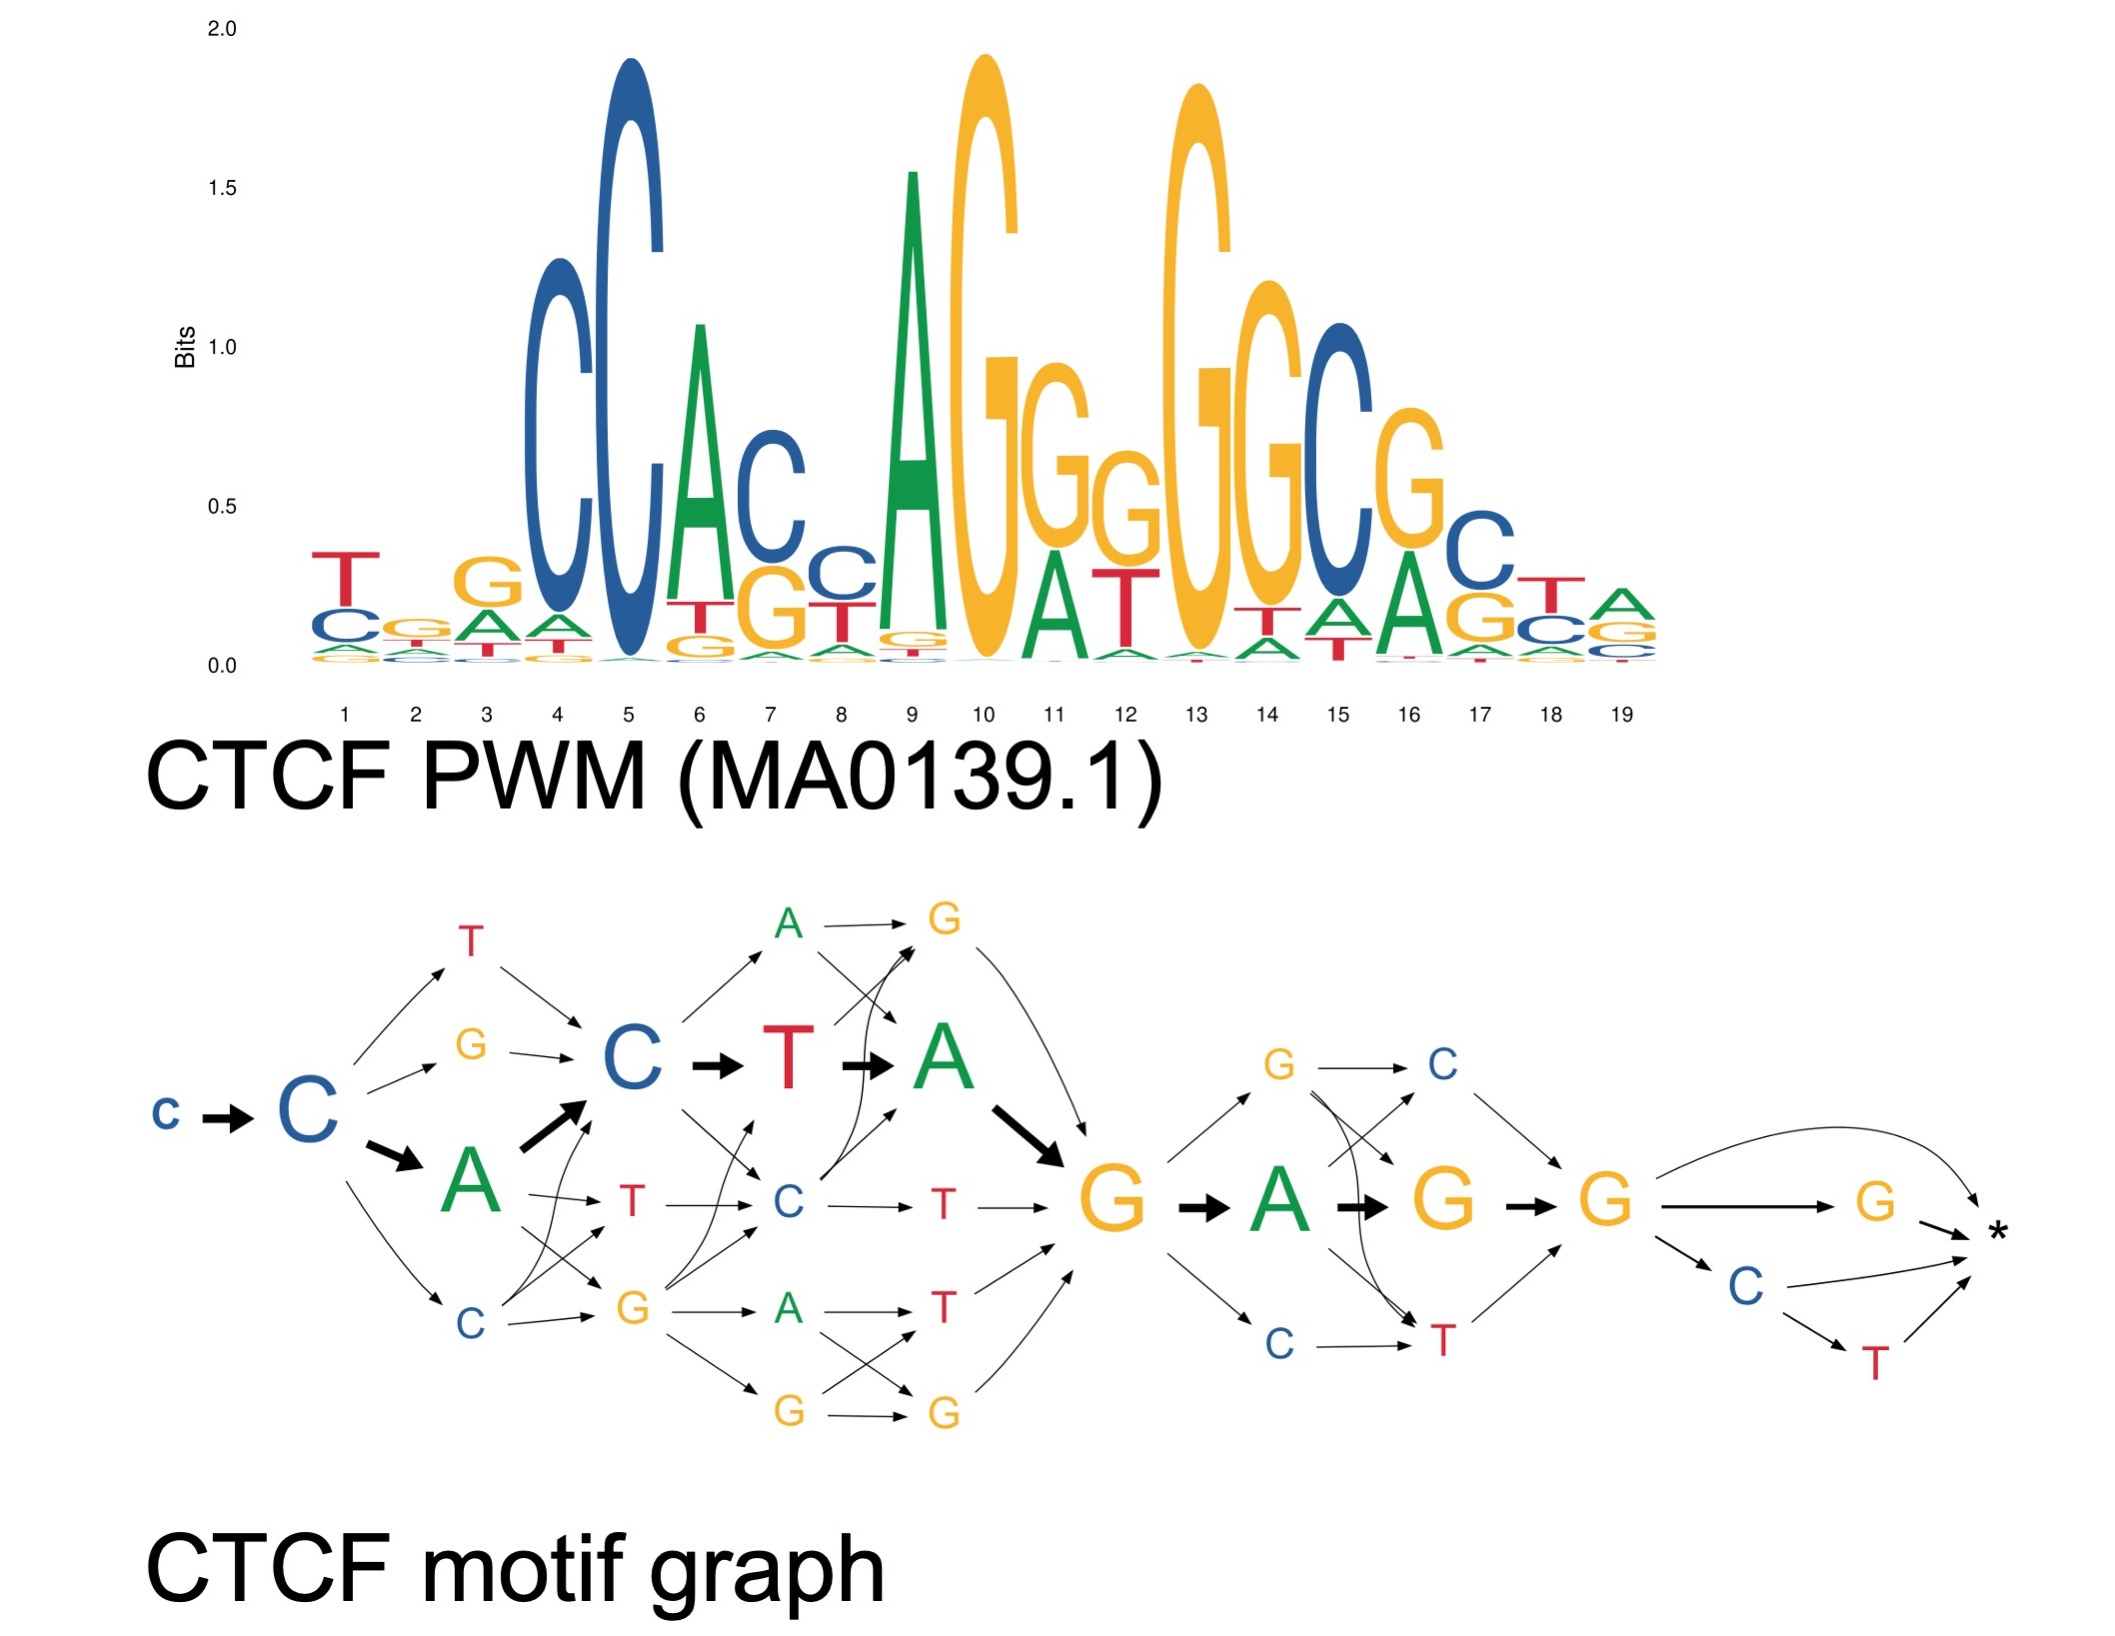
\includegraphics[width=\textwidth]{figures/ctcf_mg.jpg}
	\caption[Comparison between CTCF Motif Graph model and its PWM from the JASPAR database.]{\textbf{Comparison between CTCF MotifGraph model and its PWM from the JASPAR database.} On top the CTCF motif available on JASPAR database (MA0139.1). On the bottom the Motif Graph model trained using 100 $k$-mers obtained from a ChIP-seq experiment trageting CTCF binding site on HepG2 cell line.}
	\label{fig:ctcf_mg}
\end{figure} 
Furthermore, these models offer the potential for more accurate predictions on the imoact of non-coding variants on TF-DNA binding events and allow for the encoding of variable orders of nucleotide dependencies. Notably, graph data structures often provide interpretable and intuitive frameworks. With these goals in mind, we have developed the \motifgraph framework, which seamlessly combines the strengths of probabilistic graphical-based and SVM-based motif discovery algorithms and models. The \motifgraph model $G$ is defined by a set of vertices $V$,  edges $E$, and paths $P$. Each vertex $v \in V$ in the graph is assigned a label representing a nucleotide, denoted mathematically as \text{label}$(v) \in {A, C, G, T}$.  Meanwhile, each edge $e \in E$ denotes the allowed connections between consecutive nucleotides within the TFBS motif. Further, each path $p \in P$ corresponds to a haplotype embedded in $G$ that represents an individual sequence used to train the \motifgraph model. Currently the model is primarily designed to encode first-order dependencies between consecutive nucleotides. However, it retains the flexibility to accomodate motifs of variable lengths, all while storing essential information about the training sequences.
% ---- Motif Graph model construction
\section{Motif Graph model construction}
\motifgraph motif discovery process (\textbf{Algorithm \ref{algo:md_mg}}) encompasses two primary phases: the prioritization of $k$-mers and the training and construction of the graph model.  During the $k$-mer prioritization step, \motifgraph leverages the $k$-mer based motif discovery method proposed in LS-GKM \citep{ghandi2014enhanced, lee2016ls}. Within this framework, for each $k$-mer of length $k$ present in the positive sequence dataset $S$ and the background dataset $B$,  the algorithm tallies the number of matches in both $S$ and $B$,  accommodating mismatching positions. Subsequently, a cosine similarity kernel is trained using the frequencies of the recovered $k$-mers, with the trained kernel assigning a weight to each $k$-mer in $S$ and $B$. The $k$-mers weights reflect their influence in defining either the foreground or background dataset. The algorithm then sorts the $k$-mers based on their weight scores. The Motif Graph model undergoes an iterative training process employing a greedy approach, systematically incorporating the top-ranked $k$-mers into $G$, one by one (\textbf{Algorithm \ref{algo:mt_mg}}.) Each $k$-mer is aligned with the existing \motifgraph model, aiming to maximize the alignment of nucleotides with the current model. During this alignment process, the algorithm adjusts the input $k$-mer both to the right and left, within a specified offset number of nucleotides (a value set at 3 in our experiments). After constructing the model, we create a scoring matrix analogous to the well-known Position Specific Scoring Matrix (\emph{PSSM}), taking into account first-order nucleotide dependencies, akin to DWMs. This scoring matrix assigns a likelihood score and categorizes new sequences as potentially bound or not by the investigated factor. Essentially, the score indicates the likelihood of the scanned sequence containing a potential binding site. To score a sequence, we slide the scoring matrix along the string, employing a method akin to classical PWM scanning tools like FIMO \citep{grant2011fimo}.
\begin{algorithm}
	\DontPrintSemicolon
	\KwInput{$S$, $B$, $k$}
	\KwOutput{$G$}

	frequencies $\gets$ countFrequencies($S$, $B$, $k$)

	kernel $\gets$ trainKernel(frequencies)

	kmers, weights $\gets$ extractWeights(kernel)

	rankedKmer $\gets$ sort(kmers, weights)

	$G \gets \emptyset$

	\For{kmer in rankedKmers}
	{
		$G \gets$ addKmers($G$, kmer)
	}

	\Return{$G$}
	\caption{\textbf{Motif Graph motif discovery.}}
	\label{algo:md_mg}
\end{algorithm}
\begin{algorithm}
	\DontPrintSemicolon
	\KwInput{$G$, kmer, $i$}
	\KwOutput{$G$}
	
	\If{$i = 1$}
	{
		\Return{$G$}
	}

	\For{$j$ in $1$ to $3$}
	{
		matchesLeftOffset, alignmnetLeft $\gets$ countMatchesLeftOffset($G$, kmer, $j$)
	}

	\For{$j$ in $1$ to $3$}
	{
		matchesRightOffset, alignmnetRight $\gets$ countMatchesRightOffset($G$, kmer, $j$)
	}	
	
	alignment $\gets$ getBestAlignment(matchesLeftOffset, alignmentLeft, matchesRightOffset, alignmentRight)

	$G \gets$ insertKmer($G$, alignment)

	\Return{$G$}
	\caption{\textbf{Motif Graph model training.}}
	\label{algo:mt_mg}
\end{algorithm}
% ---- Testing the MotifGraph model
\section{ Testing the \motifgraph model}
% -- A preliminary training approach
\subsection{A preliminary training approach}
To test our motif discovery algorithm we obtained $10,000$ ChIP-seq peak sequences from the ENCODE Project database \citep{encode2012integrated} for CTCF and GATA1 obtained on the HepG2 and K562 cell lines, respectively. We sorted the ChIP-seq peaks according to their enrichment score, hence we tested our algorithm on reliable peaks. Interestingly, the trained \motifgraph models were closed to the motif PWMs on the JASPAR database \citep{sandelin2004jaspar} for both TFs (\textbf{Fig.\ref{fig:ctcf_mg}} and \textbf{Fig.\ref{fig:gata1_mg}}), capturing their consensus sequence. In the models the main motif sequences are highlighted by edge thickness, which is proportional to the number of training $k$-mers supporting each $p \in P$.
\begin{figure}
	\centering
	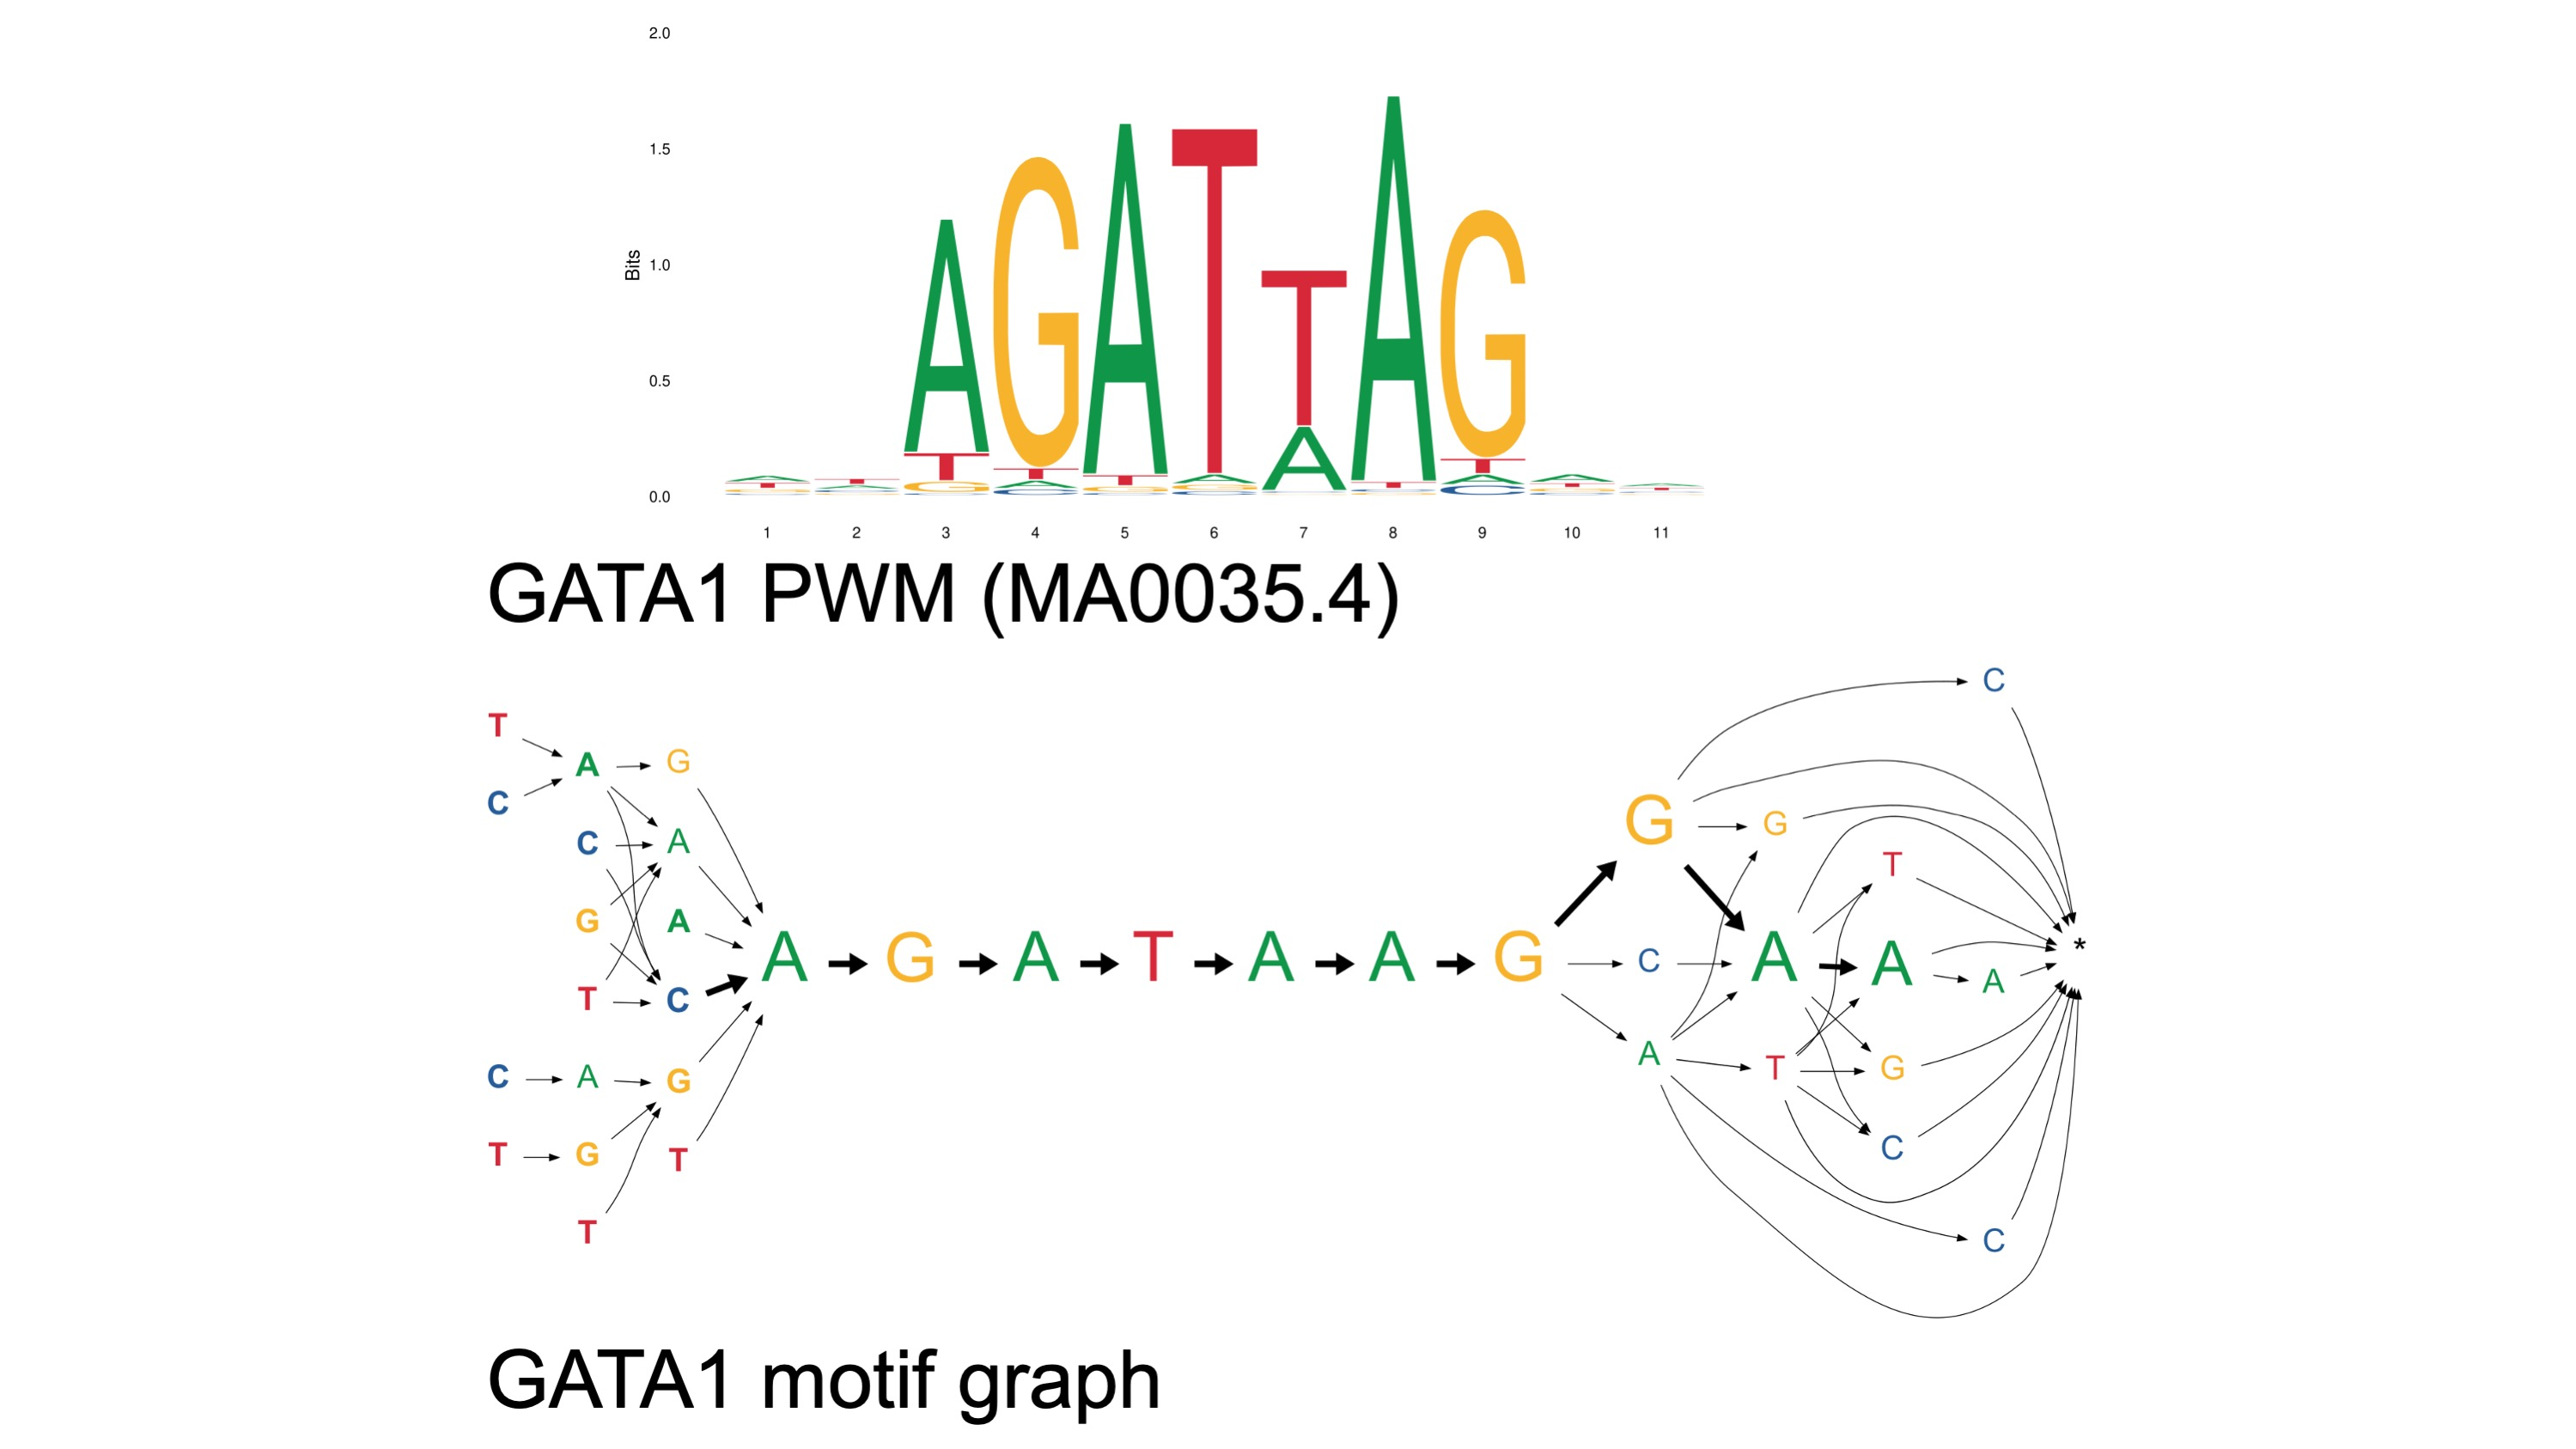
\includegraphics[width=\textwidth]{figures/gata1_mg.jpg}
	\caption[Comparison between GATA1 Motif Graph model and its PWM from the JASPAR database.]{\textbf{Comparison between GATA1 MotifGraph model and its PWM from the JASPAR database.} On top the GATA1 motif available on JASPAR database (MA0035.4). On the bottom the Motif Graph model trained using 100 $k$-mers obtained from a ChIP-seq experiment trageting GATA1 binding site on K562 cell line.}
	\label{fig:gata1_mg}
\end{figure} 
We tested the discriminative power of CTCF and GATA1 \motifgraph, training the models with different numbers of $k$-mers (\textbf{Fig.\ref{fig:dp_mg}}), to establish the optimal number of training sequences. We assessed models' discriminative power via cross-validation splitting $S$ and $B$ (75\% training and 25\%, testing). We trained the models using 10, 50, 100, 200, 350, 500, and 750 $k$-mers. For CTCF the best prformance in terms of both AUC ($0.72$) and F1-score ($0.71$) were obtained using 100 $k$-mers (\textbf{Table \ref{table:ctcf_auc_f1}}). For GATA1 the model returned the best AUC using 200 $k$-mers ($0.76$), while the best F1-score ($0.70$) was obtained training the model with $100$ sequences (\textbf{Table \ref{table:gata1_auc_f1}}).
\begin{figure}
	\centering
	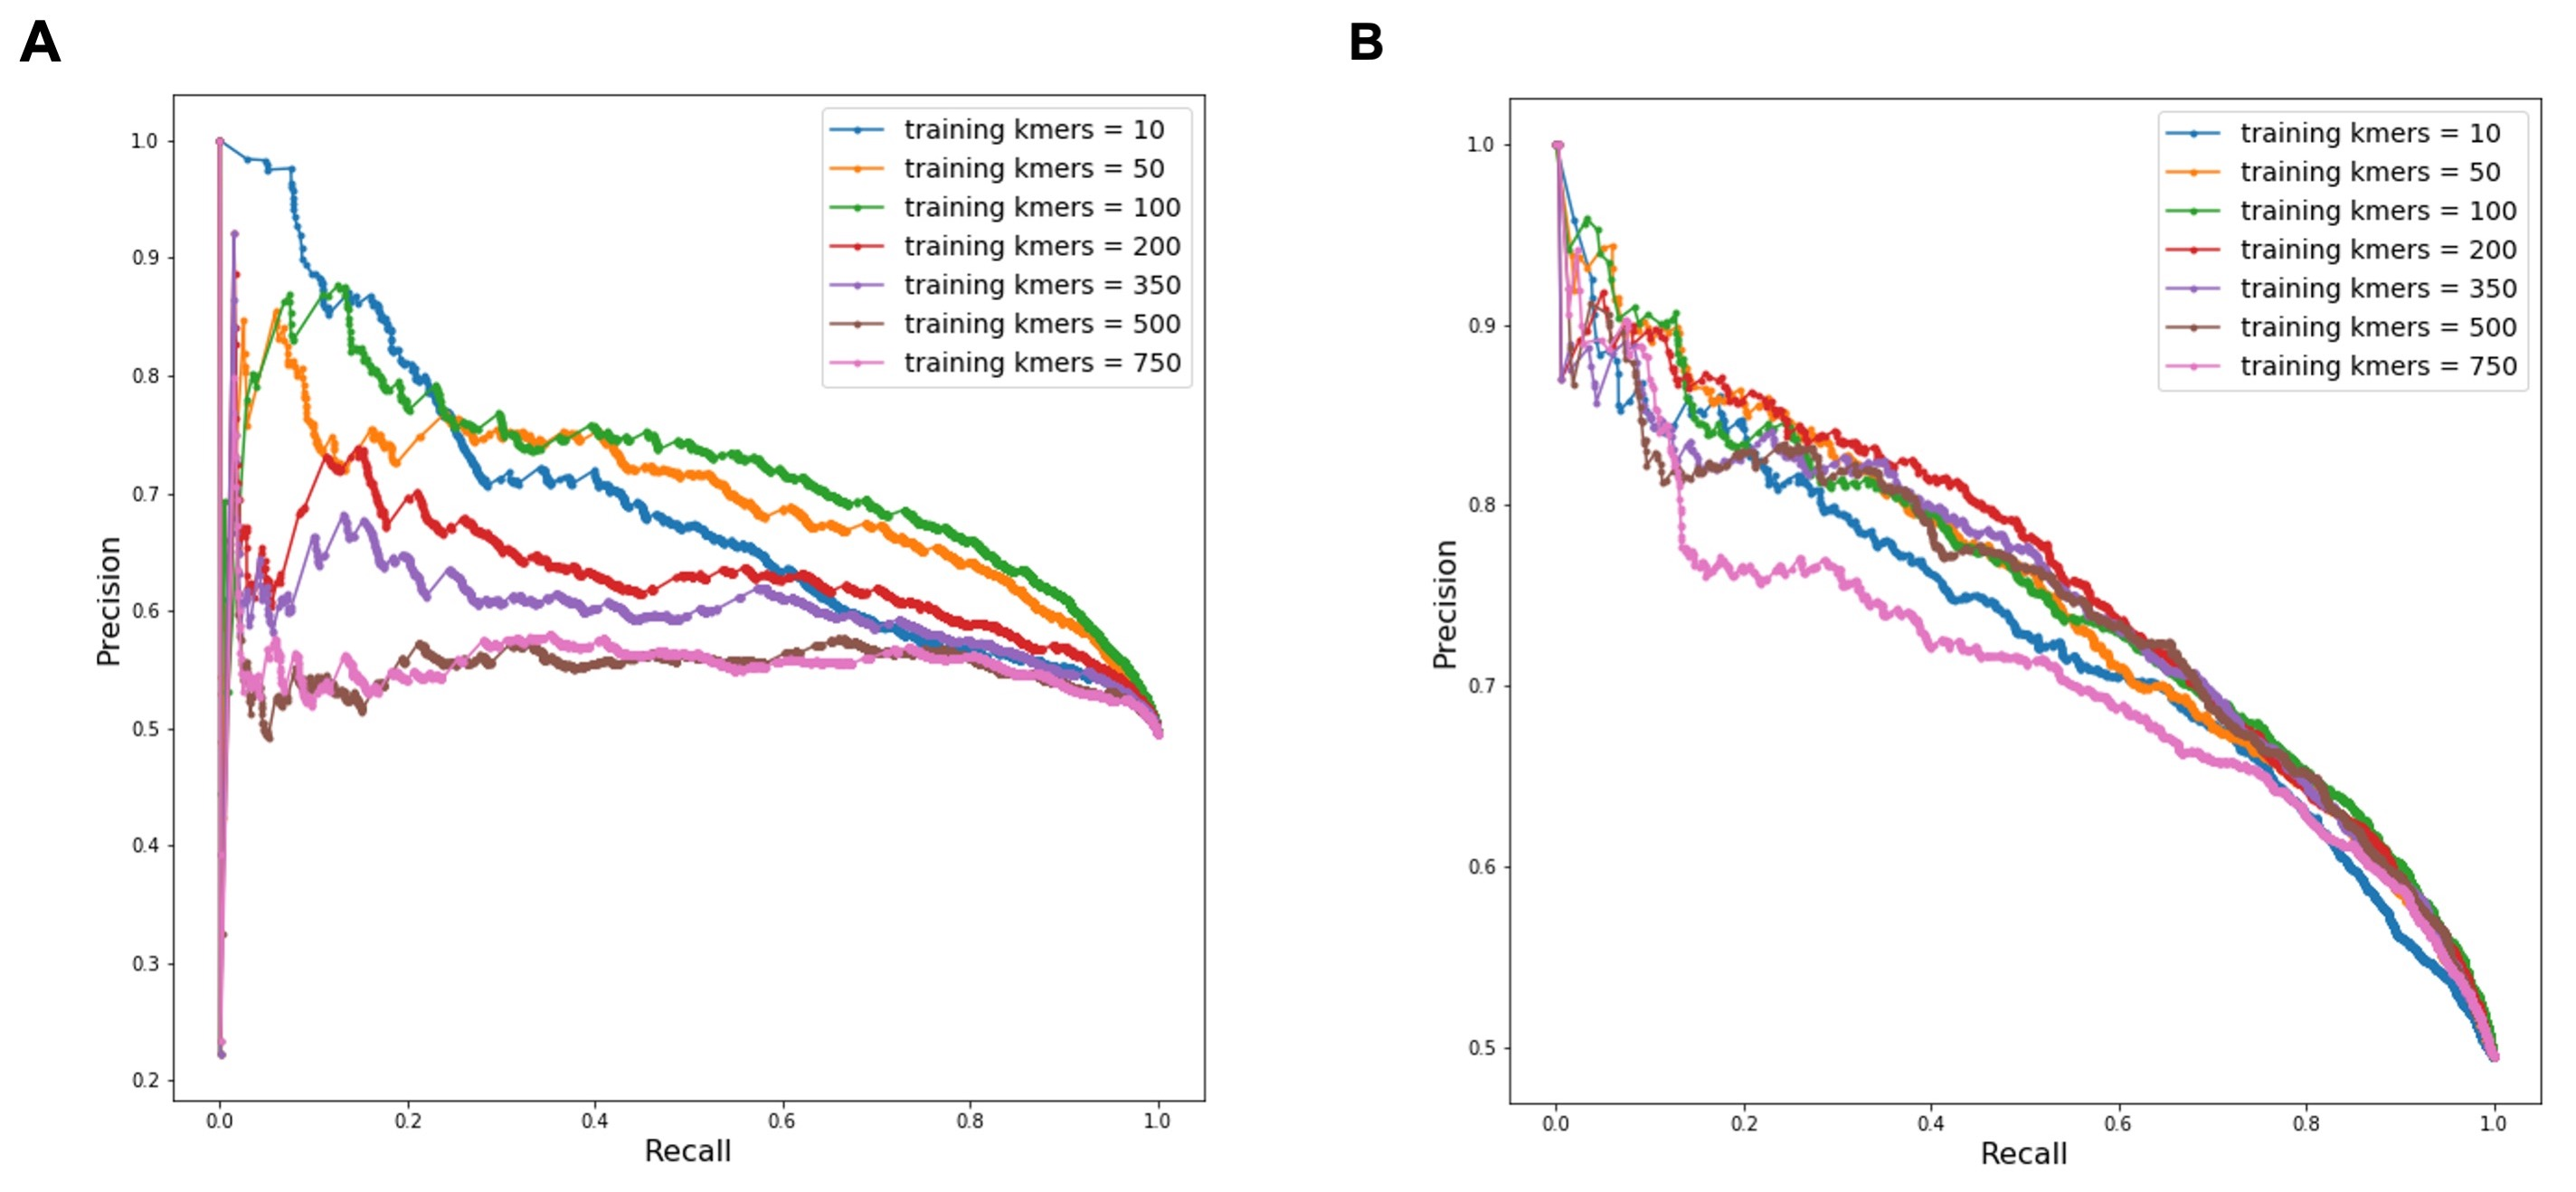
\includegraphics[width=\textwidth]{figures/dp_mg.jpg}
	\caption[Precision-Recall curves obtained varying the number of $k$-mers used to train the Motif Graph models.]{\textbf{Precision-Recall curves obtained varying the number of $k$-mers used to train the Motif Graph models.} To establish the number of training $k$-mers returning the best discriminative performance we computed the Precision-Recall curves of different Motif Graph models trained using 10, 50, 100, 200, 350, 500, and 750 $k$-mers on \textbf{(A)} CTCF and \textbf{(B)} GATA1}
	\label{fig:dp_mg}
\end{figure} 
\begin{table}
	\centering
	\begin{tabular}{|p{3cm}|p{1.cm}|p{1.cm}|p{1.cm}|p{1.cm}|p{1.cm}|p{1.cm}|p{1.cm}|}
		\hline
		\textbf{Training $k$-mers}& \textbf{$10$}& \textbf{$50$}& \textbf{$100$}& \textbf{$200$}& \textbf{$350$}& \textbf{$500$}& \textbf{$750$} \\
		\hline
		\textbf{AUC}& $0.69$& $0.69$& $0.72$& $0.63$& $0.60$& $0.55$& $0.55$\\
		\hline
		\textbf{F1-score}& $0.62$& $0.69$& $0.71$& $0.65$& $0.62$& $0.57$& $0.56$\\
		\hline
	\end{tabular}
	\caption[CTCF Motif Graph model AUC and F1-scores values with different number of training $k$-mers.]{\textbf{CTCF Motif Graph model AUC and F1-scores values with different number of training $k$-mers.}}
	\label{table:ctcf_auc_f1}
\end{table}
\begin{table}
	\centering
	\begin{tabular}{|p{3cm}|p{1.cm}|p{1.cm}|p{1.cm}|p{1.cm}|p{1.cm}|p{1.cm}|p{1.cm}|}
		\hline
		\textbf{Training $k$-mers}& \textbf{$10$}& \textbf{$50$}& \textbf{$100$}& \textbf{$200$}& \textbf{$350$}& \textbf{$500$}& \textbf{$750$} \\
		\hline
		\textbf{AUC}& $0.73$& $0.75$& $0.75$& $0.76$& $0.74$& $0.74$& $0.71$\\
		\hline
		\textbf{F1-score}& $0.68$& $0.68$& $0.70$& $0.69$& $0.70$& $0.69$& $0.67$\\
		\hline
	\end{tabular}
	\caption[GATA1 Motif Graph model AUC and F1-scores values with different number of training $k$-mers.]{\textbf{GATA1 Motif Graph model AUC and F1-scores values with different number of training $k$-mers.}}
	\label{table:gata1_auc_f1}
\end{table}
We also compared \motifgraph models discriminative power against the corresponding PWMs and DWMs downloaded from JASPAR \citep{sandelin2004jaspar} and HOCOMOCO \citep{kulakovskiy2016hocomoco}, respectively. For CTCF, both PWM and DWM showed better performance than our model (\textbf{Fig.\ref{fig:dp_mg_pwm_dwm} (A)}). On the other hand, on GATA1 data our model behaved better than PWMs, although it still performed worse than DWMs (\textbf{Fig.\ref{fig:dp_mg_pwm_dwm} (B)}).
\begin{figure}
	\centering
	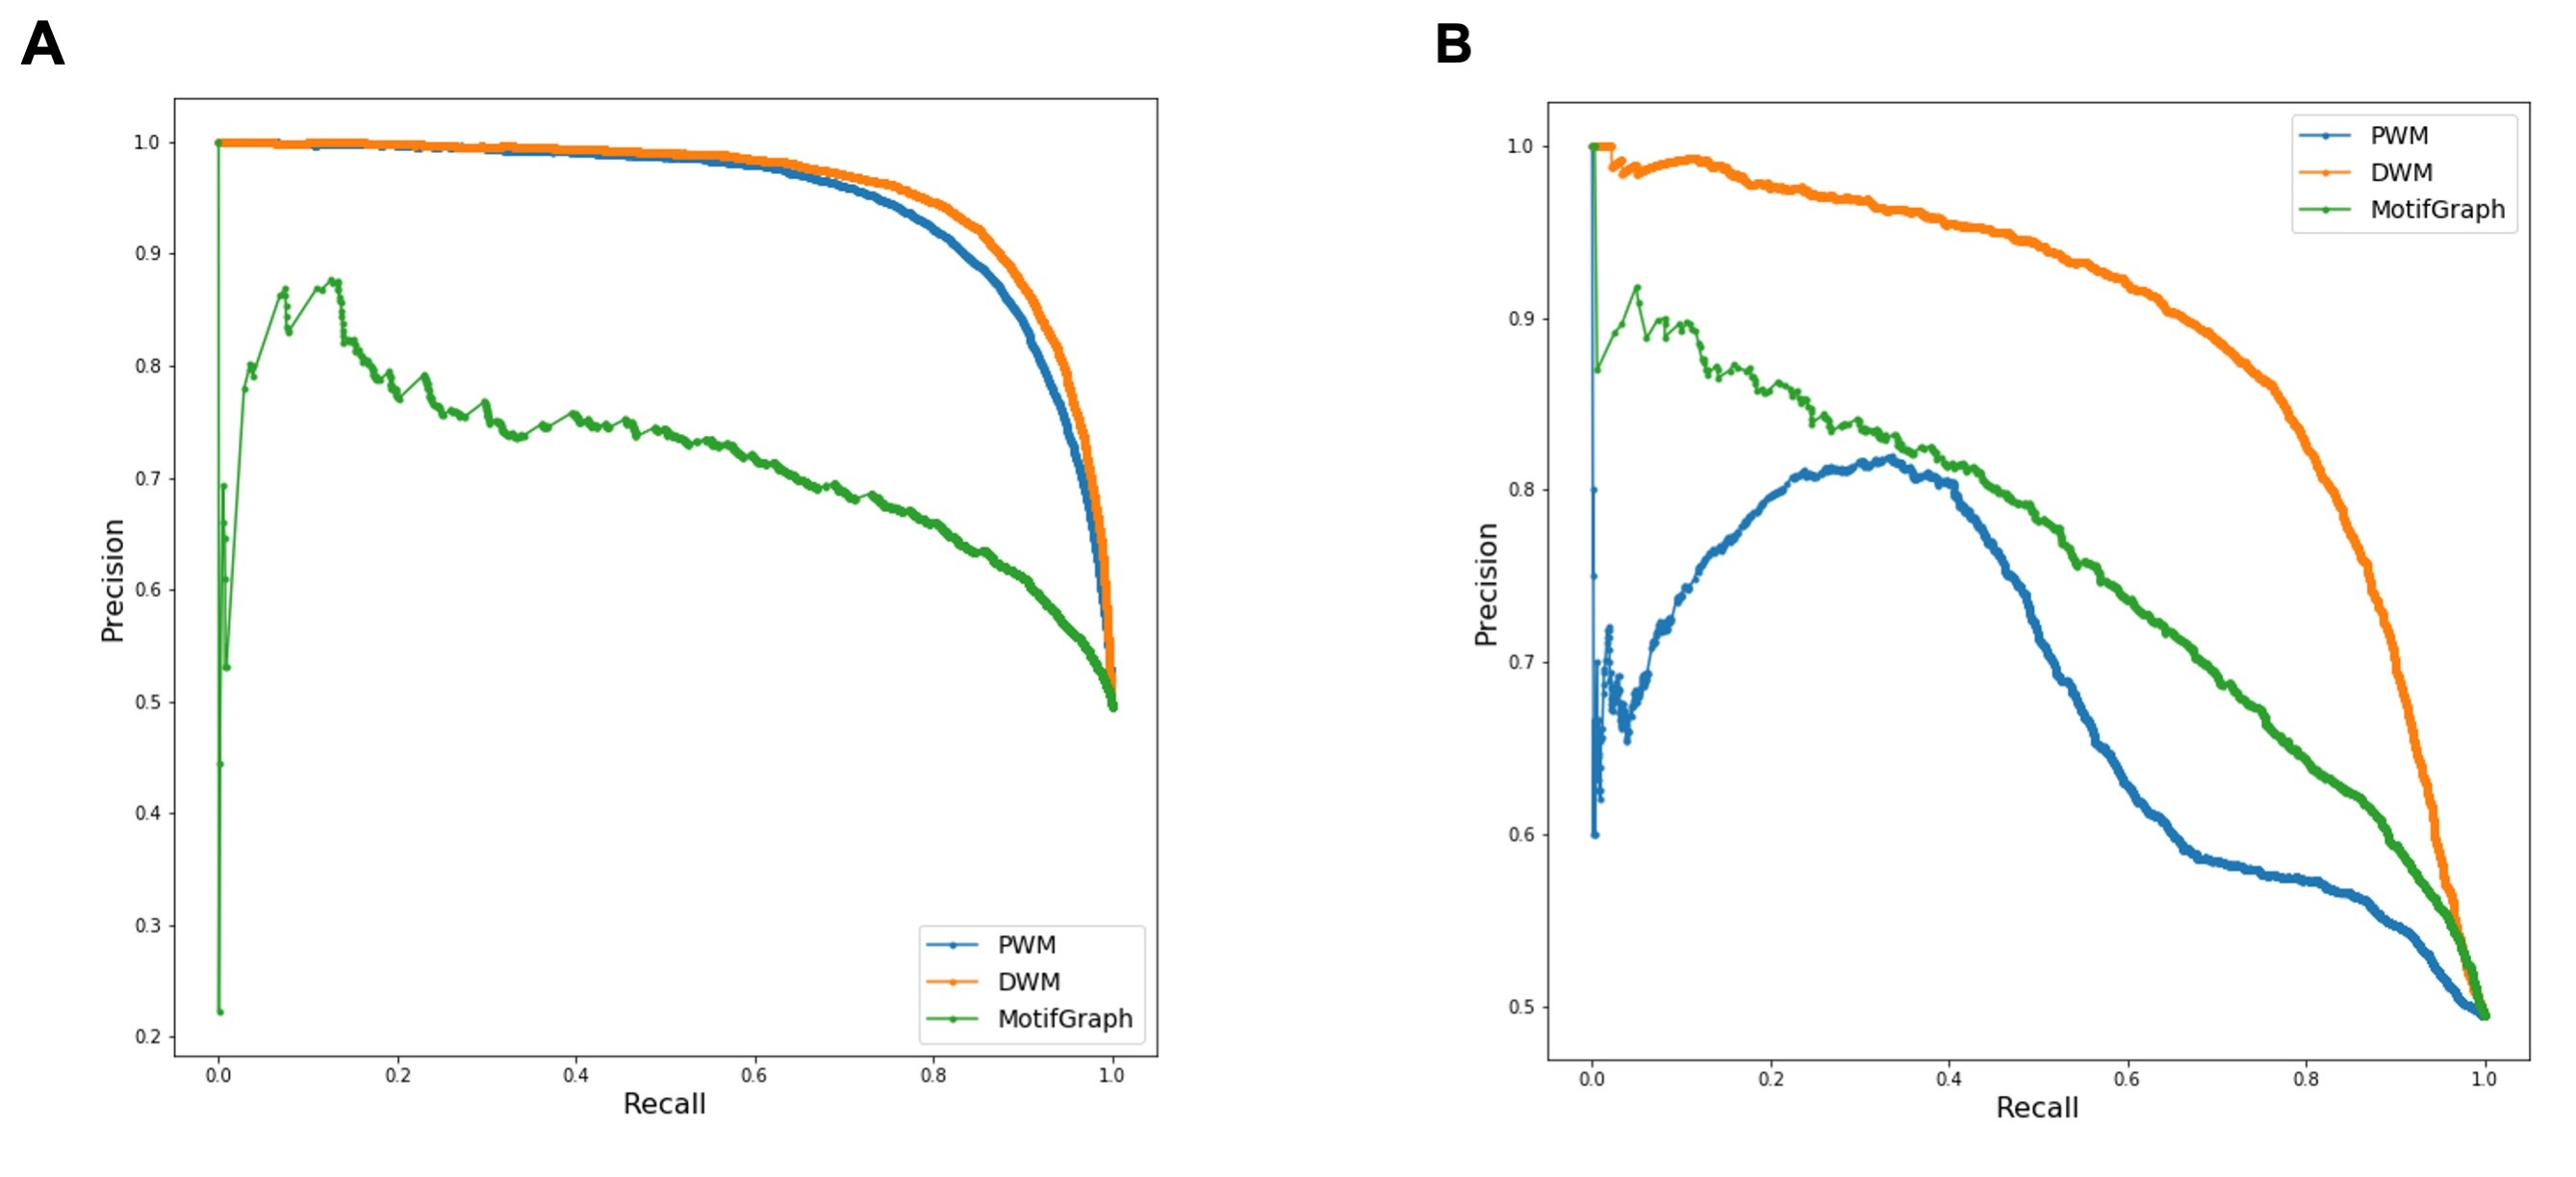
\includegraphics[width=\textwidth]{figures/dp_mg_pwm_dwm.jpg}
	\caption[Comparing Motif Graph, PWM, and DWM Precision-Recall curves.]{\textbf{Comparing Motif Graph, PWM, and DWM Precision-Recall curves.} We compared the discriminative power of the Motif Graph models against that of PWMs and DWMs for both \textbf{(A)} CTCF and \textbf{(B)} GATA1.}
	\label{fig:dp_mg_pwm_dwm}
\end{figure} 
% -- Improving k-mers prioritazion
\subsection{Improving $k$-mers prioritazion}
To improve the performance of our models we focused on improving $k$-mers selection procedure.  To this goal in mind, we developed a $k$-mers prioritazition procedure similar to LS-GKM algorithm. Given $S$ and $B$, we compute gapped $k$-mers frequencies for each sequence in the input datasets. Using the gapped $k$-mers frequencies we compute a cosine similarity matrix measuring cosine similarity between each sequence pair in $S$ and $B$.  We then identify potential sequence clusters running the Leiden algorithm \citep{traag2019louvain} on a graph $G_{L}$ constructed from the cosine similarity matrix. $G_{L}$ is defined by a set of vertices $V$ and edges $E$, where each $v \in V$ is a sequence in $S$ and $B$, $e \in E$ is a term of comparison between two sequences, and \text{weight}$(e)$ is the cosine similarity value between the two sequences linked by $e$. We then train a \motifgraph $G$ with ech sequence cluster separately.  To test our procedure we used CTCF ChIP-seq peak sequences on K562 cell lines for $S$, while $B$ was obtained by shuffling the sequences in $S$, maintaining first-order dependencies.By plotting the cosine similarity matrix using UMAP we observe two clear clusters separating foreground (bound) and background (unbound) sequences (\textbf{Fig.\ref{fig:motifgraph1} (A)}). Furthermore, the clusters correlates with the binding affinity scores computed running FIMO \citep{grant2011fimo} on the sequences in $S$ and $B$ (\textbf{Fig.\ref{fig:motifgraph1} (B)}).
\begin{figure}
	\centering
	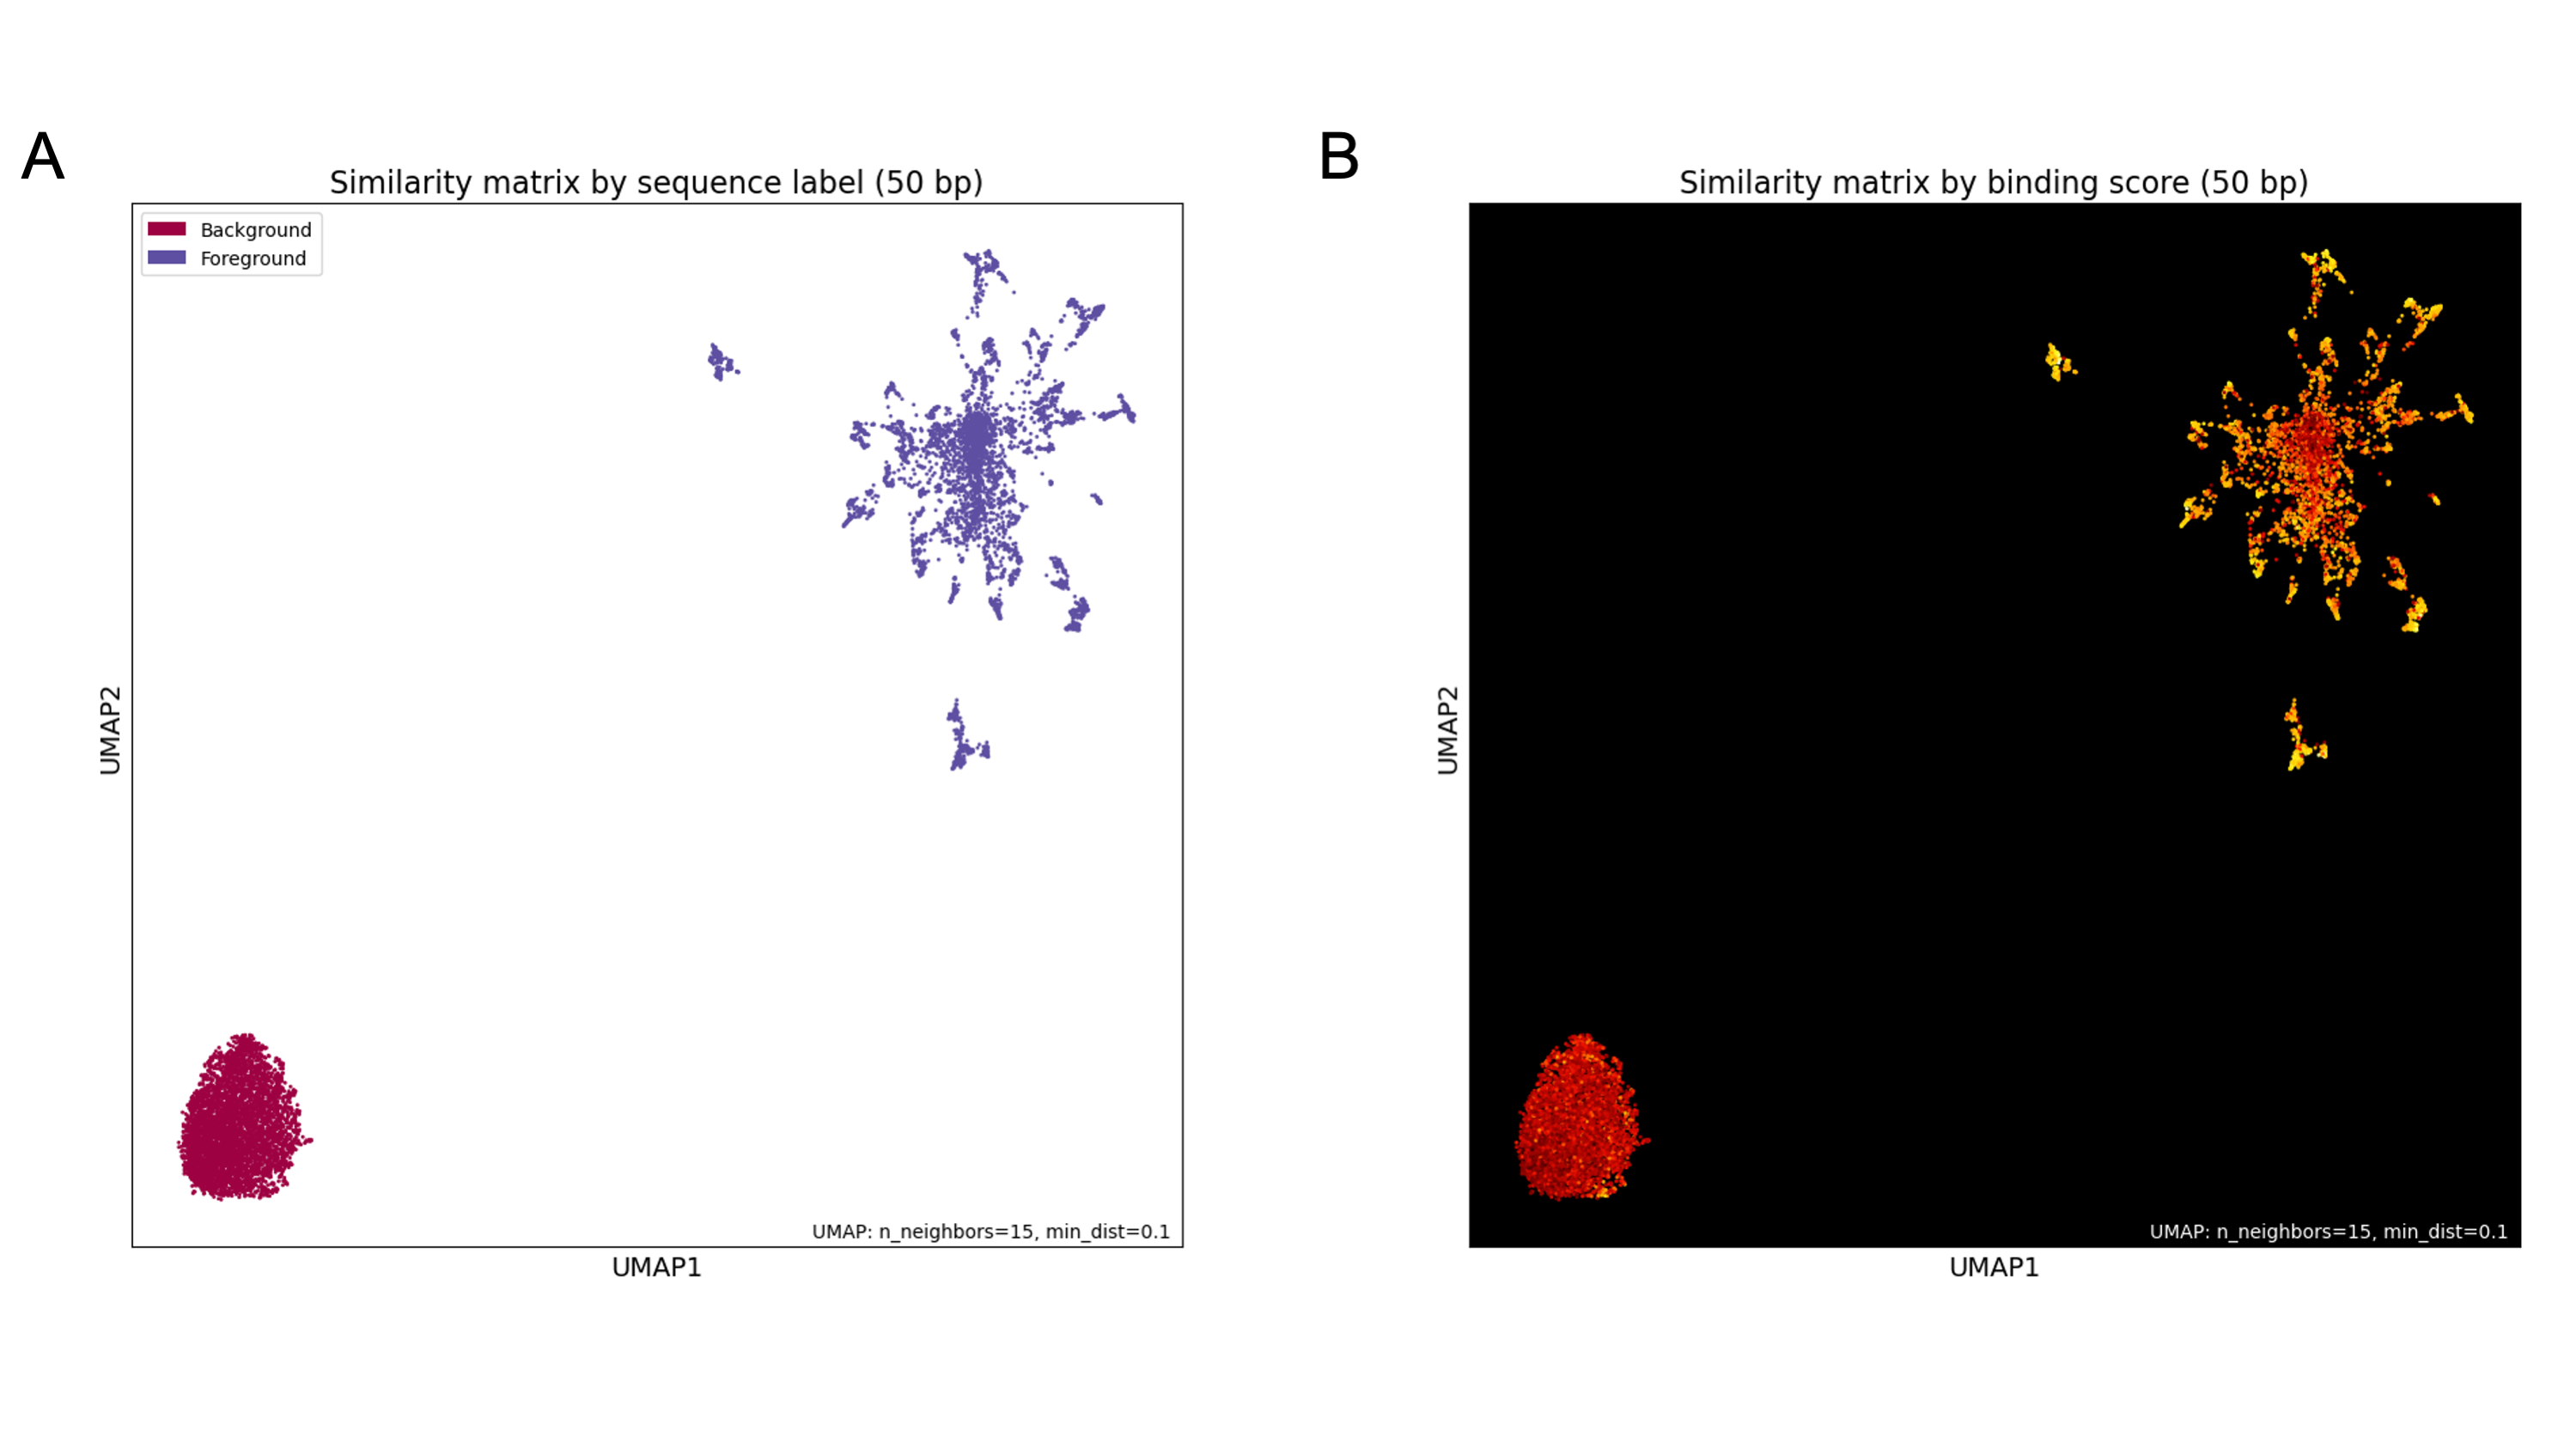
\includegraphics[width=\textwidth]{figures/motifgraph1.png}
	\caption[UMAP plot of foreground and background sequence clusters]{\textbf{UMAP plot of foreground and background sequence clusters. (A)} Plotting the cosine similarity matrix with UMAP computed on CTCF ChIP-seq data (cell line K562) the foreground and background sequence clusters are identified. \textbf{(B)} The  clusters correlates with the binding affinity scores computed on the sequences running FIMO.}
	\label{fig:motifgraph1}
\end{figure} 
\begin{figure}
	\centering
	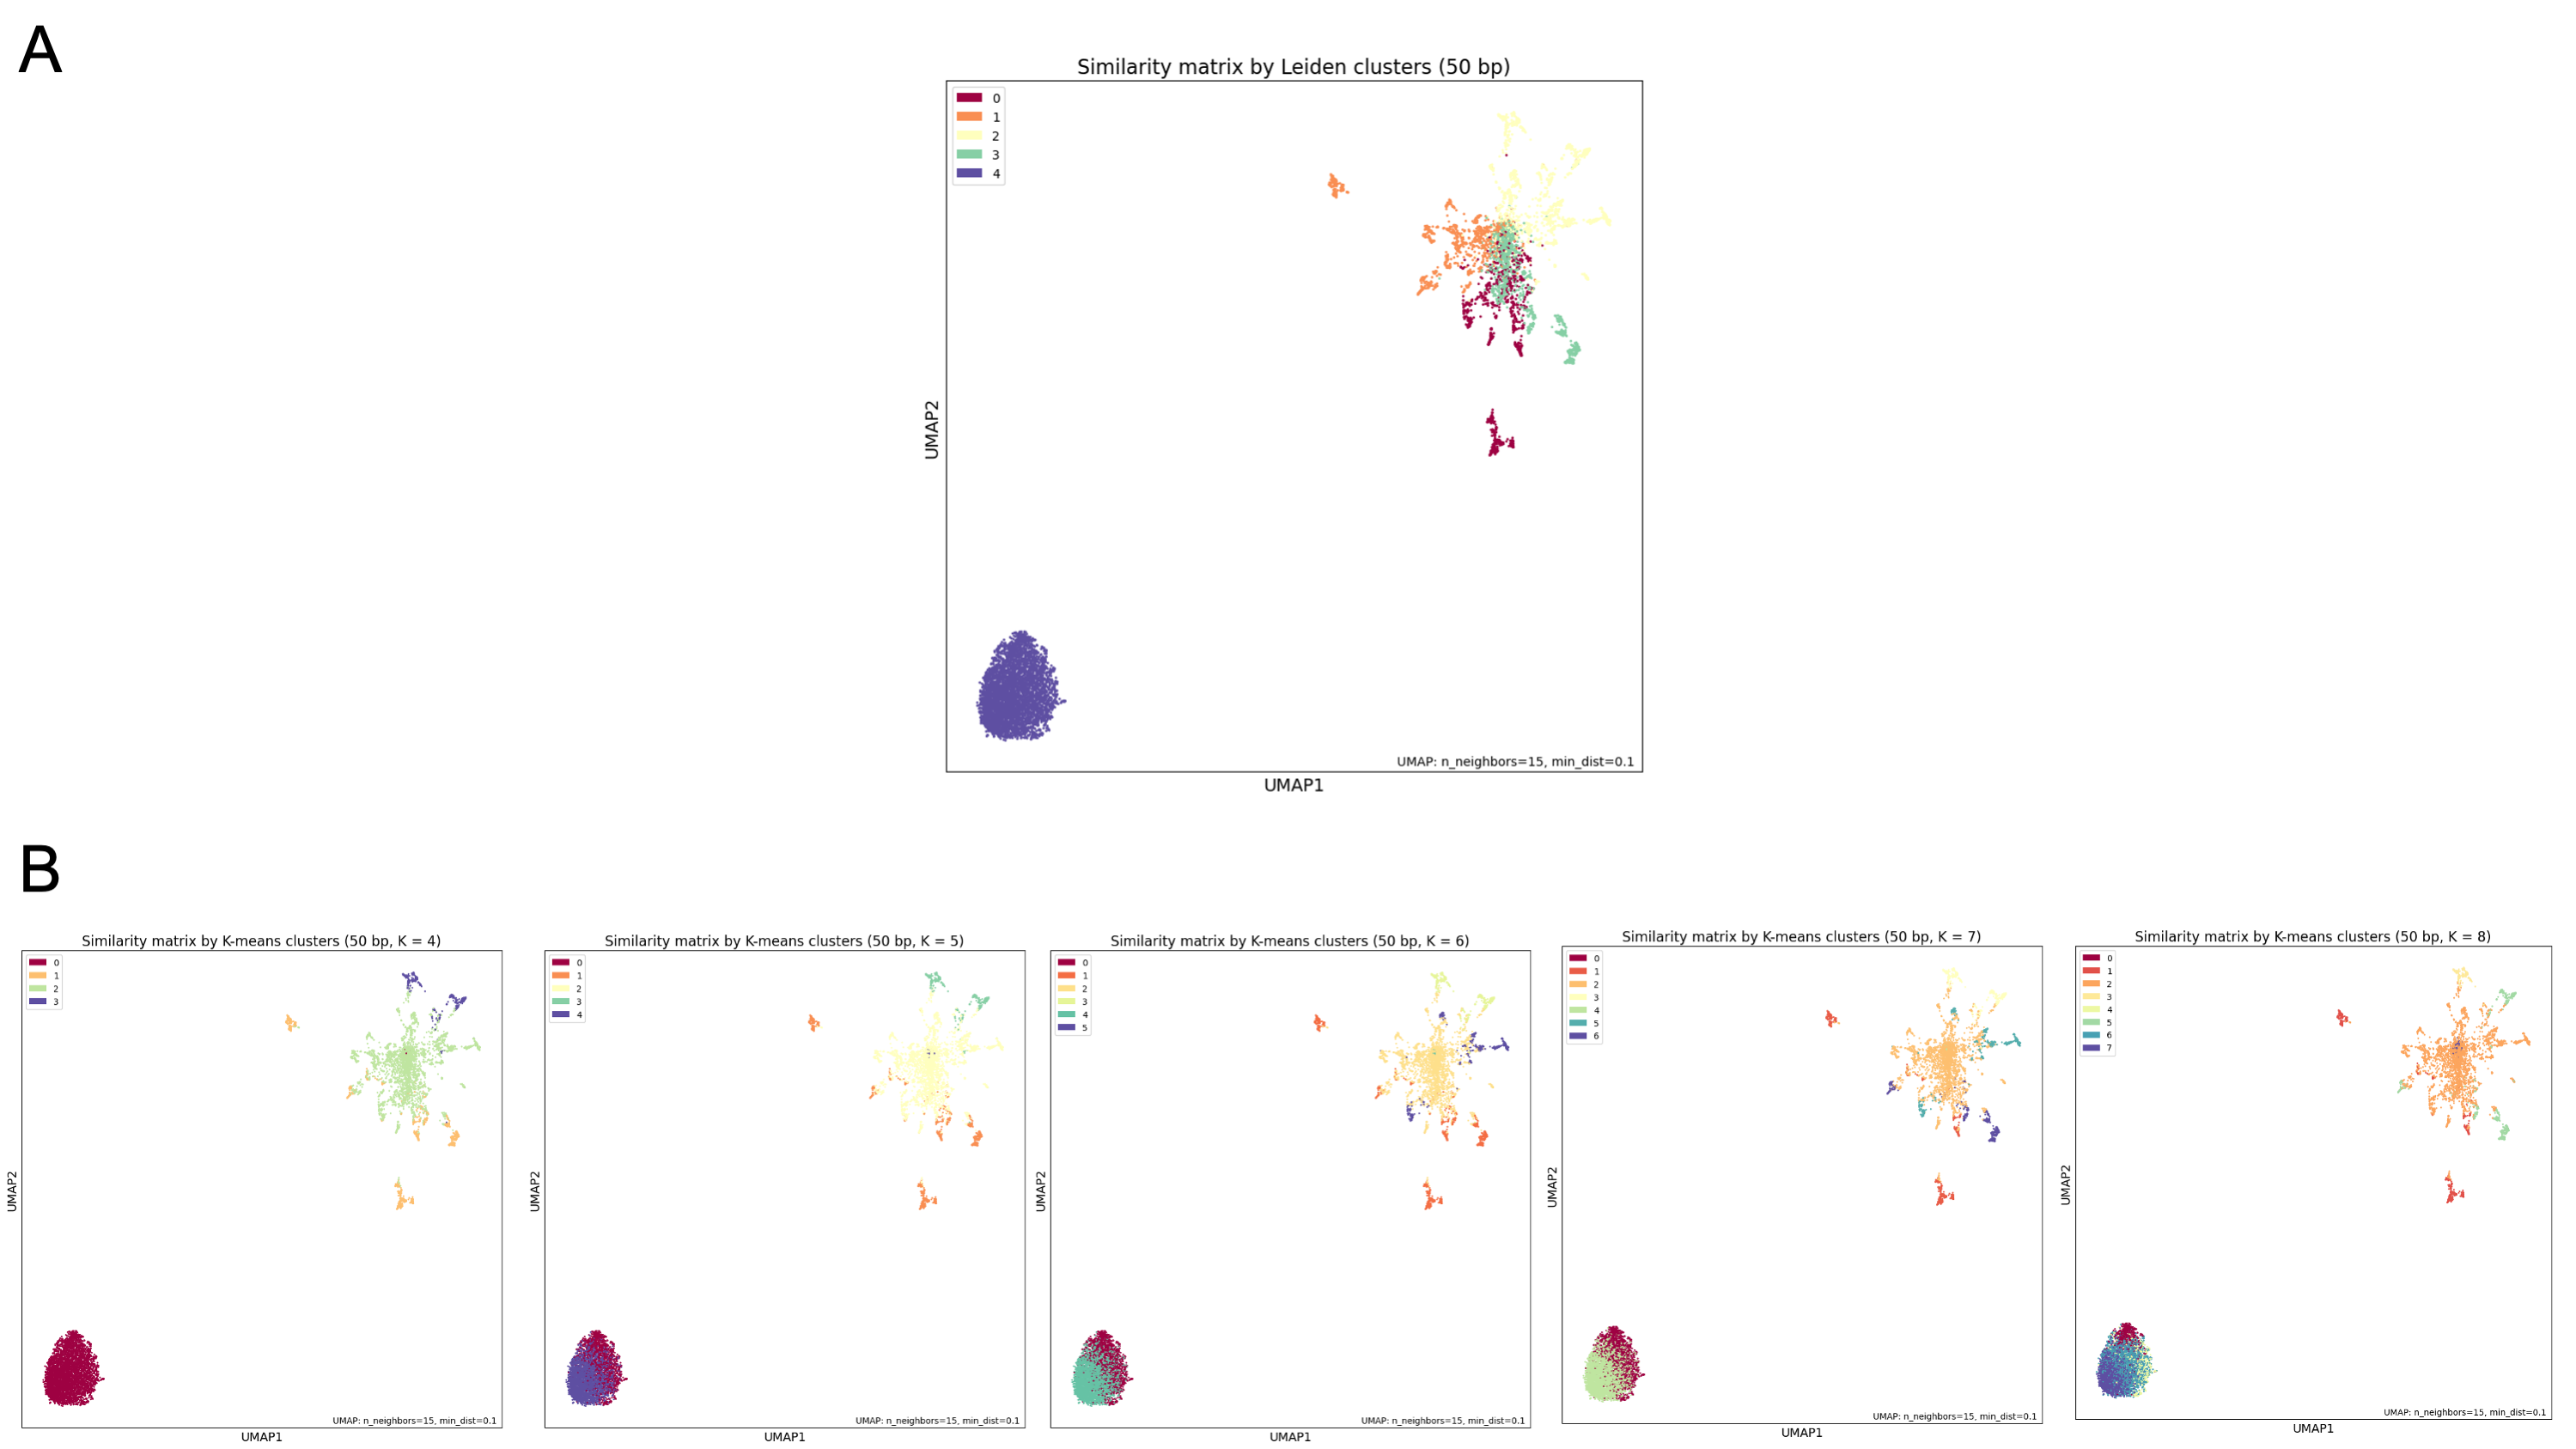
\includegraphics[width=\textwidth]{figures/motifgraph2.png}
	\caption[Leiden algorithm identifies five clusters]{\textbf{Leiden algorithm identifies five clusters. (A)} Running the Leiden algorithm on $G_{L}$ identifies five clusters. While it keeps background sequences in a single cluster, it splits foreground sequences in four different clusters. \textbf{(B)} $K$-means clustering identifies different sequence clusters and often splits even the background sequences cluster.}
	\label{fig:motifgraph2}
\end{figure} 

By running Leiden algorithm on $G_{L}$, it identifies five different clusters. While it keeps the background sequences in a single cluster, the foreground sequences are divided in four clusters (\textbf{Fig.\ref{fig:motifgraph2} (A)}).  To assess Leiden's results, we run $k$-means on the cosine similarity matrix using $k \in {4,5,6,7,8}$. However, increasing $k$ the algorithm split even the background sequences in different clusters, suggesting poor clustering performance \textbf{Fig.\ref{fig:motifgraph2} (B)}).
% -- Future directions
\section{Future directions}
In the next future we plan to construct the \motifgraph using the sequences prioritized by the Leiden algorithm in a cluster-wise fashion. , We expect that different cluster will return different motifs,  corresponding to different motif grammars recovered from different genomic regions. That enforces our initial aim of providing a comprehensive model learning different features in a single framework.
% ------- Predicting genetic variants impact on transcription factor binding sites
\mychapter{5}{Predicting genetic variants impact on transcription factor binding sites}
Many have highlighted the significant influence of genetic variations on TF-DNA binding events \citep{de2006regulatory, weinhold2014genome, guo2018mutation}. Genome-wide association studies (GWASs) have revealed thousands of genetic variants, known as single nucleotide polymorphisms (SNPs), that are associated with complex human traits. Notably, these SNPs are typically situated within noncoding regions of the genome, many of which function as regulatory elements such as enhancers \citep{maurano2012systematic} Consequently, SNPs have the potential to influence gene expression by modulating TF-DNA interactions. These genetic variants can disrupt TF-DNA binding sequences, potentially leading to alterations in downstream gene expression patterns \citep{deplancke2016genetics}. Crucially, mutations that affect transcription factor binding sites (TFBS) can persist within specific haplotypes found in populations \citep{kasowski2010variation},, contributing to the emergence of population-specific TFBS. Similarly, genetic variability between cell types can give rise to cell-type-specific TF target sequences. Therefore, it becomes imperative to develop software tools capable of predicting the potential impact of genetic variations on TFBS specificity, while also considering haplotype and cell-type-specific mutations.  In pursuit of this goal, we have introduced two tools designed for predicting the effects of mutations on TFBS within haplotypes and across different cell types. \grafimo \citep{tognon2021grafimo} is a variant- and haplotype-aware motif scanning tool searching potential occurrences of known TF motifs on genome graphs \citep{paten2017genome}. Briefly, genome graphs are graph-based data structures, where nodes correspond to DNA sequences and edges describe allowed links between successive sequences. Paths through the graph, which may be labelled (such as in the case of a reference genome), correspond to haplotypes belonging to different genomes \citep{siren2020haplotype} (\textbf{Fig.\ref{fig:vg}}). \motifraptor \citep{yao2021motif} investigates the imapct of genetic variants on TFBS interpolating different omics data, such as cell type-specific transcriptomic data and chromatin accessibility. In particular, \motifraptor is designed to support researchers while annotating variants located within non-coding regions, and provides a potential functional annotation for these mutations. In our research we extend the current \motifraptor to employ SVM-based motif models (\textbf{section 2.1.2}), which often provide better predictions on variants impact than PWM models \citep{tognon2023survey}.

\begin{figure}
	\centering
	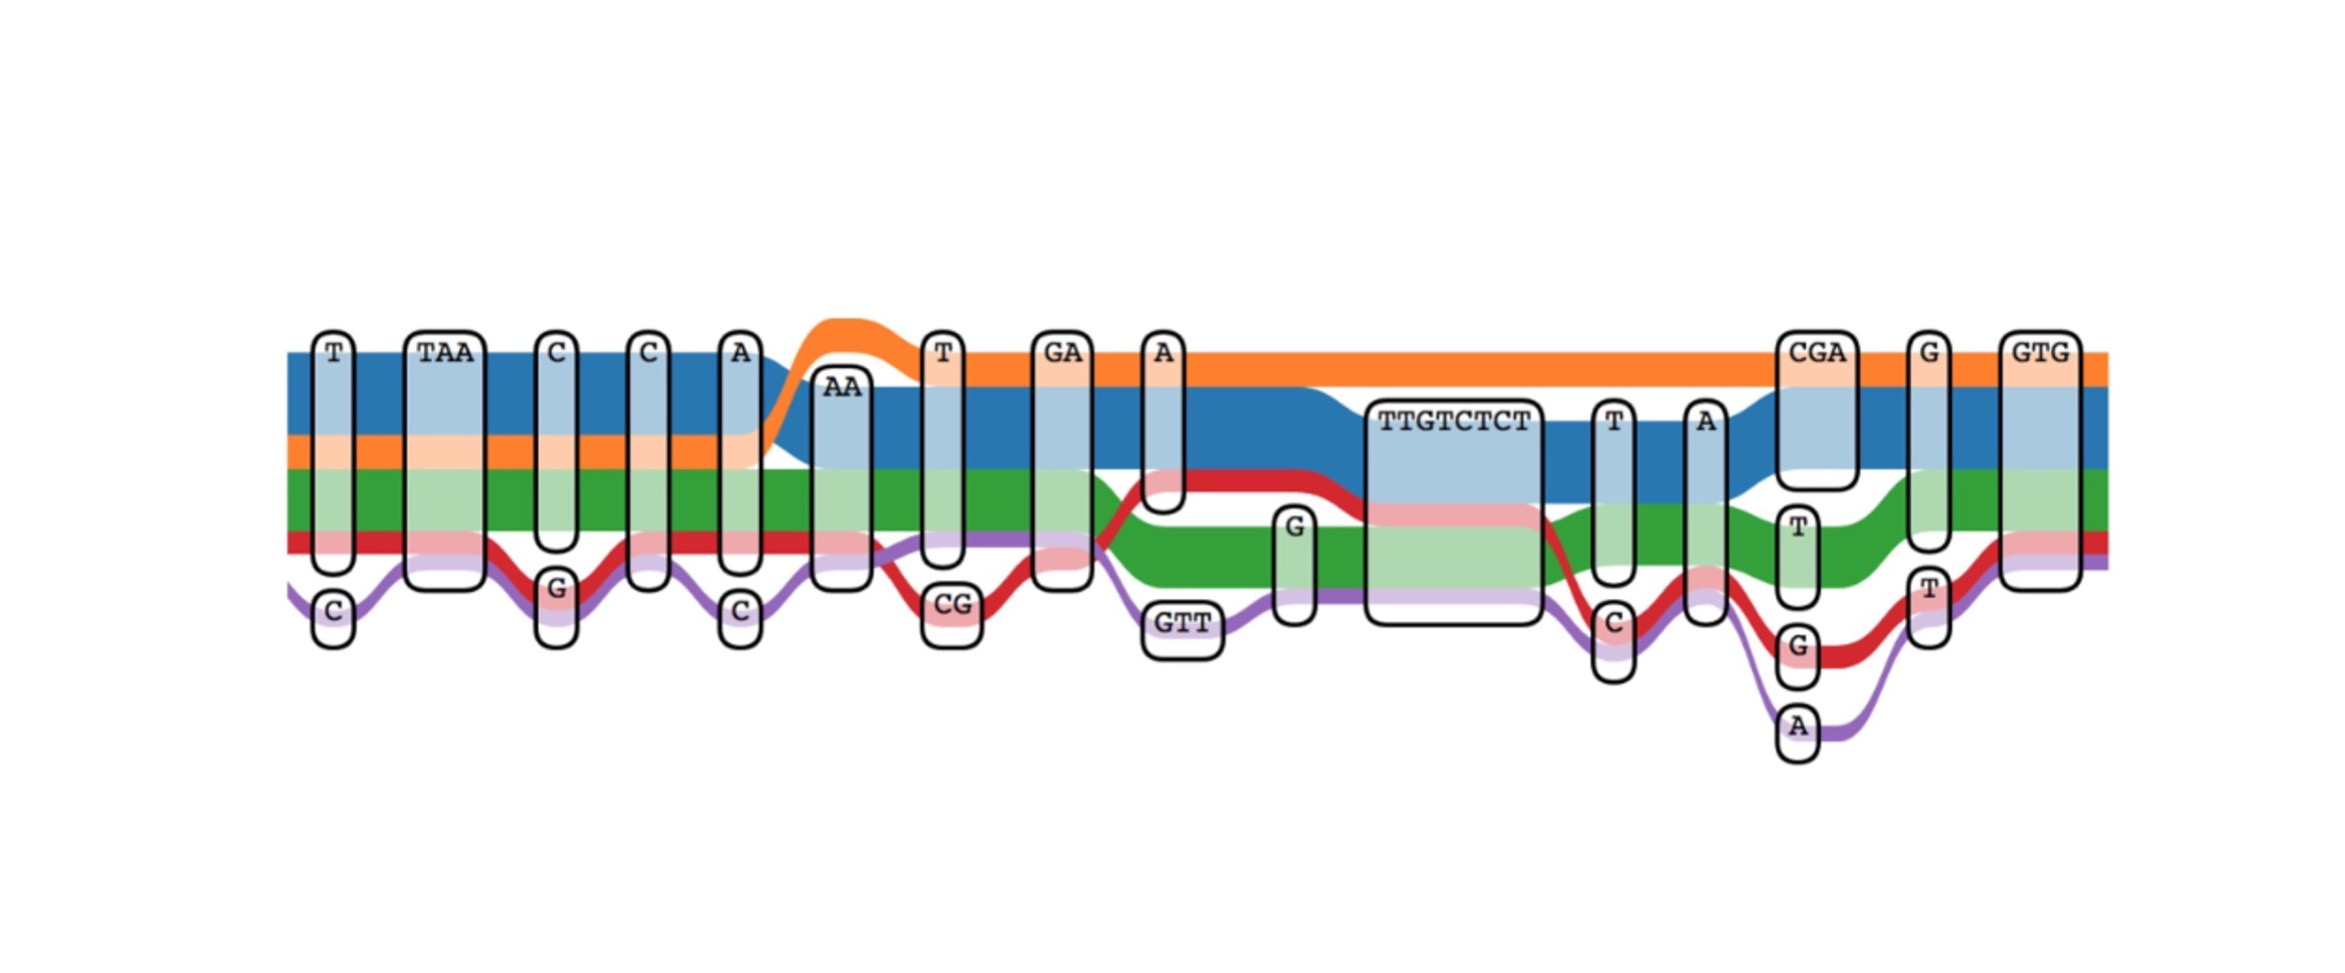
\includegraphics[width=\textwidth]{figures/vg.jpg}
	\caption[Genome Graphs data structure visualization]{\textbf{Genome Graphs data structure visualization.}  Each color corresponds to a path in the graph. Each path represents the genomic sequences of one of the individual genomes encoded in the Genome Graph structure.}
	\label{fig:vg}
\end{figure} 
% ---- GRAFIMO
\section{GRAFIMO}
% In recent years, several tools have been proposed for scanning regulatory DNA regions, such as enhancers or promoters, with the goal of predicting which TF may bind these genomic locations. Importantly, it has been shown that regulatory motifs are under purifying selection \citep{li2015human,  vorontsov2016negative}, and mutations occurring in these regions can lead to deleterious consequences on the transcriptional states of a cell \citep{guo2018mutation}. In fact, mutations can weaken, disrupt or create new TFBS and therefore alter expression of nearby genes. Mutations altering TFBS can occur in haplotypes that are conserved within a population or private to even a single individual, and can correspond to different phenotypic behaviour \citep{kasowski2010variation}. For these reasons, population-level analysis of variability in TFBSs is of crucial importance to understand the effect of common or rare variants to gene regulation. Recently, a new class of methods and data structures based on genome graphs have enabled us to succinctly record and efficiently query thousands of genomes.  Genome graphs optimally encode shared and individual haplotypes based on a population of individuals. An efficient and scalable implementation of this approach called variation graphs (VGs) has been recently proposed \citep{garrison2018variation}.  VGs offer new opportunities to extend classic genome analyses originally designed for a single reference sequence to a panel of individuals. Moreover, by encoding individual haplotypes, VGs have been shown to be an effective framework to capture the potential effects of personal genetic variants on functional genomic regions profiled by ChIP-seq of histone marks \citep{groza2020personalized} 
Over the past decade, significant strides have been made in the development of methods to search known TFBS on linear reference genomes \citep{tognon2023survey, boeva2016analysis}. Notable examples include FIMO \citep{grant2011fimo} and MOODS \citep{korhonen2009moods}. They scan a set of genomic sequences searching for potential occurrences of known TFBS represented as PWMs. Additionally, tools such as is-rSNP, TRAP, and atSNP \citep{macintyre2010rsnp, thomas2011transcription, zuo2015atsnp} were introduced to accommodate SNPs and short indels in the sequences to scan. However, these tools fall short in considering individual haplotypes and providing summaries of the frequency of these events in a population. To address these challenges, we developed \grafimo (GRAph-based Finding of Infividual Motif Occurrences) \citep{tognon2021grafimo}, a novel tool designed to offer a variant- and haplotype aware identification of known TFBS in genome graphs. We demonstrate the utility of \grafimo by searching TFBS on a genome graph encoding the haplotypes from all individuals sequenced by the 1000 Genomes Project (1KGP) \citep{siva20081000, zheng2017alignment}. This innovative approach provides a more nuanced understanding of TF-DNA interaction dynamics in the context of population-wide genetic diversity.

% -- Design and implementation
\subsection{Design and implementation}
\grafimo is a command-line tool enabling an efficient variant- and haplotype-aware search of known TFBS, within a population of individuals encoded in a genome graph. \grafimo provides two main functionalities: genome graph construction from user data, and the search of one or more TFBS motifs on input precomputed graphs. Briefly, given a TF motif PWM and a set of genomic regions, \grafimo leverages genome graphs to efficiently scan and report all the TFBS candidates and their frequencies in a single pass. Along with the motif candidates, \grafimo reports the predicted changes in binding affinity mediated by the genetic variants embedded in the graph. \grafimo is written in Python3 and Cython and it has been designed to interface with \emph{vg} toolkit to handle genome graphs.

% ---- Genome graph construction
\subsubsection{Genome variation graph construction}
\grafimo offers an intuitive command-line interface for constructing genome graphs from user data, when needed. Given a reference genome (FASTA format) and a set of genomic variants (VCF format), \grafimo seamlessly interfaces with the \emph{vg} toolkit to build the genome graphs (\texttt{VG} format) and its indexes (\texttt{XG} \citep{garrison2018variation} and \texttt{GBWT} \citep{siren2020haplotype, novak2017graph} formats). The two indexes are required to perform efficient graph traversal and track the haplotypes embedded in the data structure. To minimize the footprint of the genome graph files, \grafimo construct a graph per chromosome. Moreover, this graph construction design speeds-up the TFBS motif search by allowing to scan different chromosomes in parallel. Alternatively, for systems with limited RAM, the search can be conducted one chromosome at a time, providing flexibility in resource usage.

% ---- Transcription factor binding site motif search
\subsubsection{Transcription factor binding site motif search}
The TFBS motif search in \grafimo requires a set of genomes embedded in a genome graph (\texttt{XG} format), a database of known TF motif PWMs, and a set of genomic regions (BED format). \grafimo reports all the potential TFBS motif occurrences found in the input regions and their associated statistical significance (\textbf{Fig.\ref{fig:grafimo1}}). To identify potential TFBS, \grafimo employs a sliding window approach with a window length of $k$, where $k$ is the query motif width. The window traverses the paths in the graphs that correspond to the genome sequences encoded in it (\textbf{Fig.\ref{fig:grafimo1}(B)}). This process is accomplished by an extension to the \texttt{vg find} functionality, using the graph's \texttt{GBWT} index to explore the $k$-mer space, while considering the embedded haplotypes \citep{siren2020haplotype}. By default, \grafimo focuses its search on paths corresponding to observed haplotypes, but it also provides an option to consider all possible recombinants, even if absent in any embedded sample. The significance (log-likelihood) of each TFBS candidate is determined by evaluating the nucleotide preferences encoded in the motif PWM, akin to FIMO \citep{grant2011fimo}. Specifically, the PWM undergoes processing into a Position Specific Scoring Matrix (PSSM) (\textbf{Fig.\ref{fig:grafimo1}(A)}). The resulting PSSM log-likelihood values are scaled within the range $[0, 1000]$. The scaling allows efficient statistical significance ($P$-value) computations via dynamic programming \citep{grant2011fimo}. Subsequently $P$-values undergo conversion to $q$-values through the Benjamini-Hochberg procedure to correct for multiple hypothesis testing. In this procedure, all $P$-values correspond to all the $k$-mer-paths extracted within the scanned graph's regions. Additionally, \grafimo provides insights into the number of haplotypes in which a significant motif is observed, along with its presence in the reference genome and/or alternative genomes (\textbf{Fig.\ref{fig:grafimo1}(B)}). 

% - figure: GRAFIMO TF motif search workflow
\begin{figure}
	\centering
	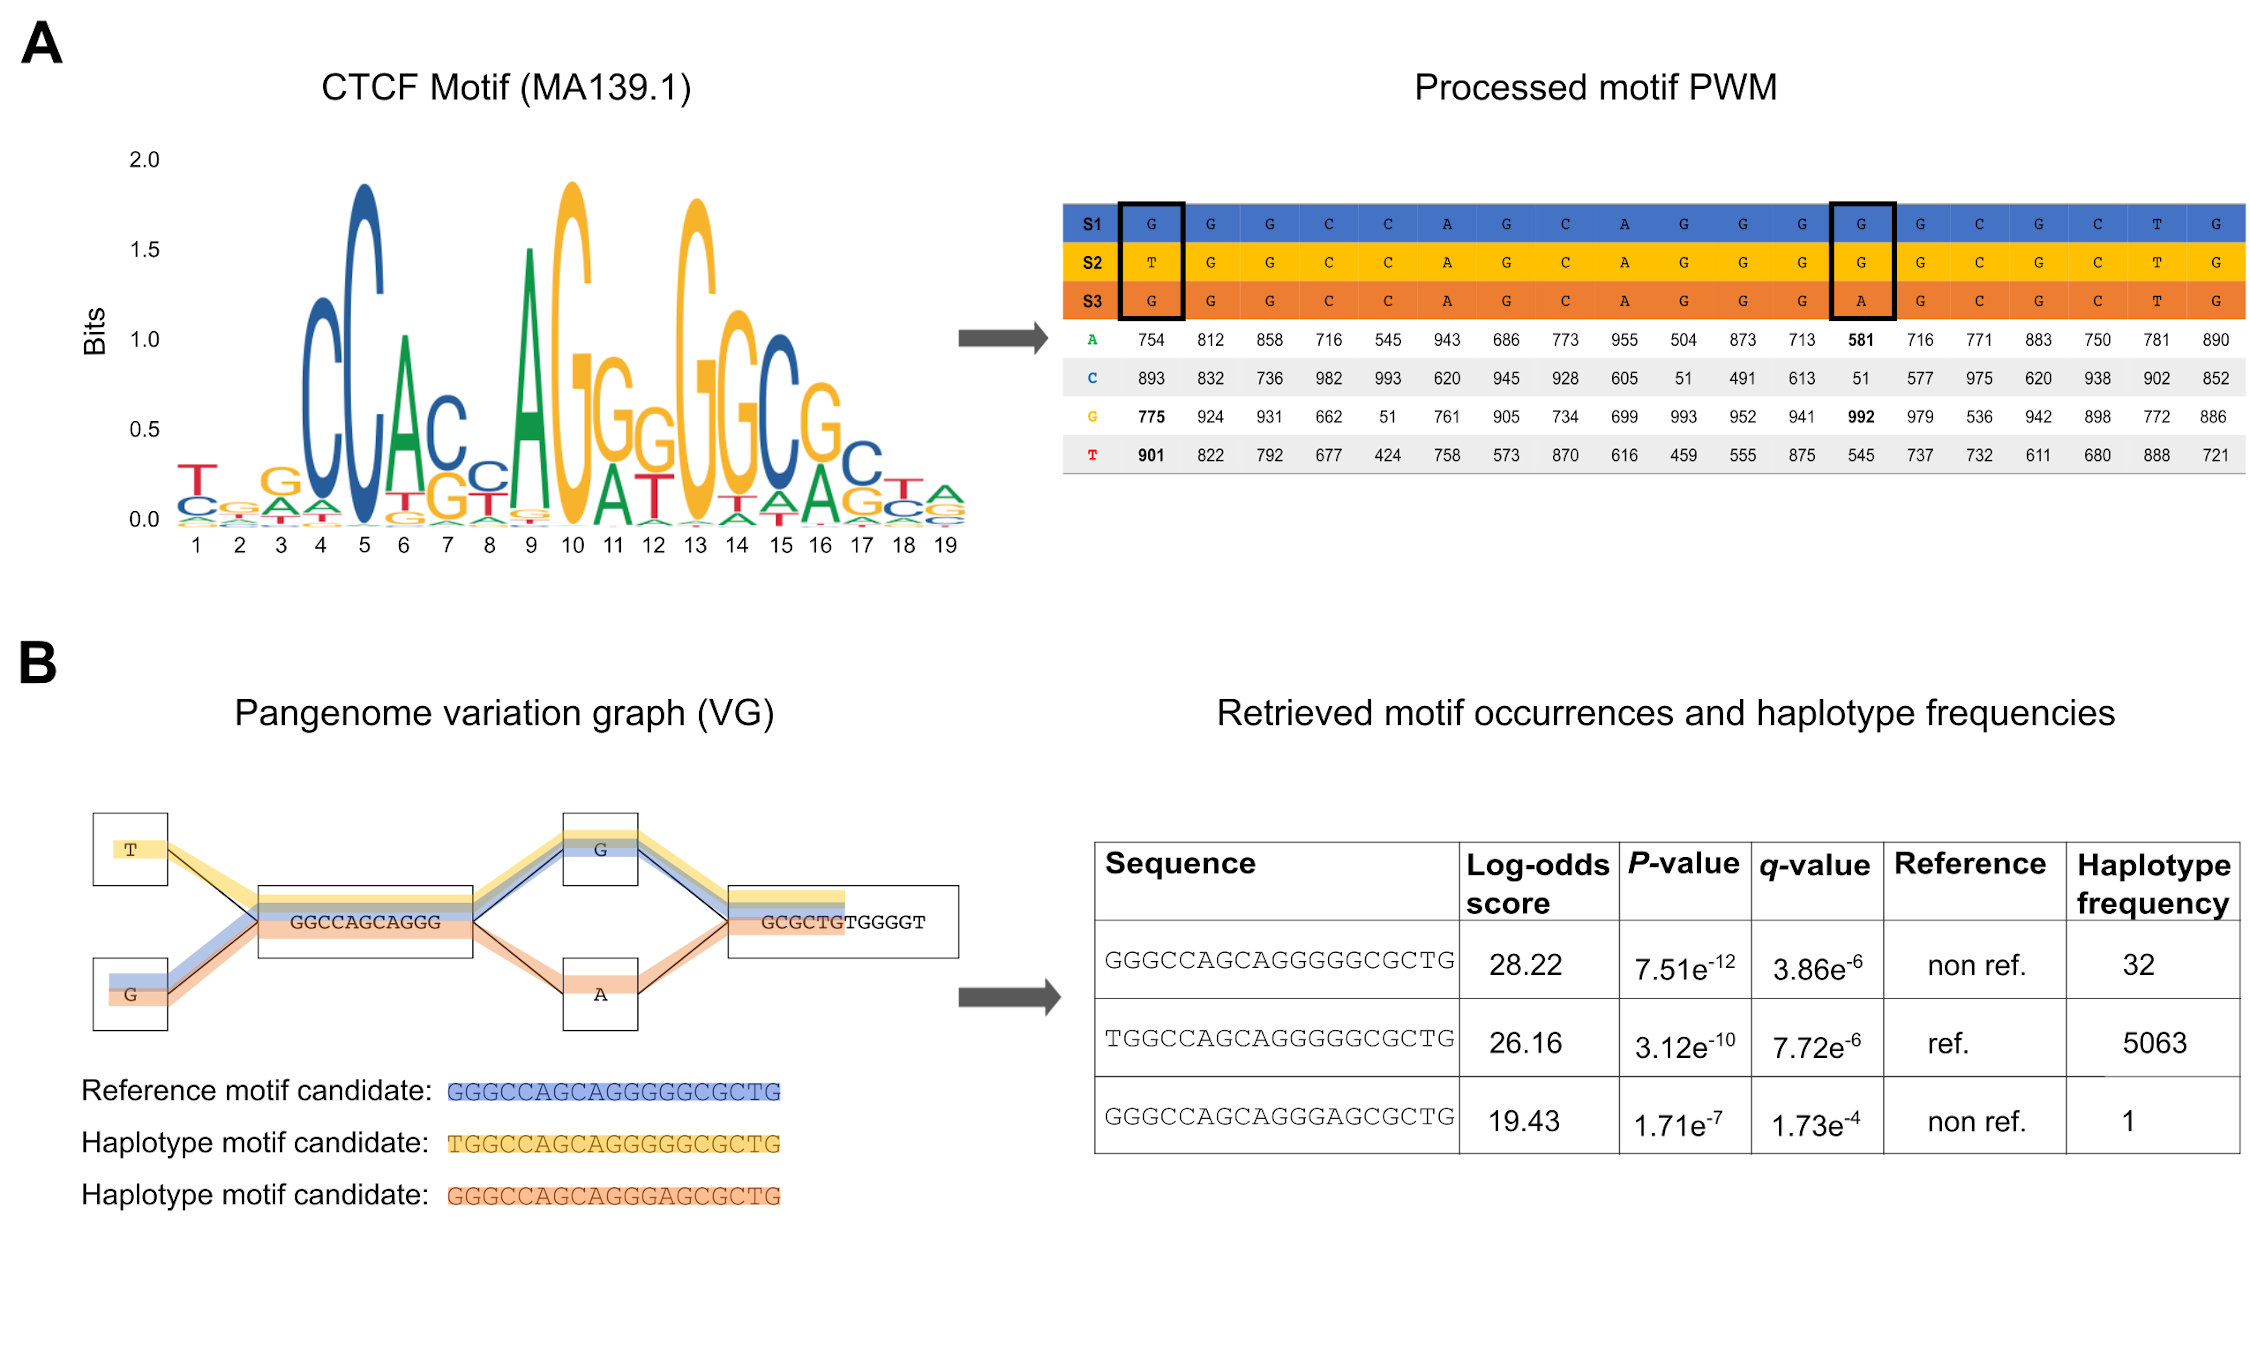
\includegraphics[width=\textwidth]{figures/grafimo1.png}
	\caption[GRAFIMO TF motif search workflow.]{\textbf{\grafimo TF motif search workflow. (A)} The motif PWM (in MEME or JASPAR format) is processed and its values are scaled in the range [0, 1000]. The resulting score matrix is used to assign a score and a corresponding P-value to each motif occurrence candidate. In the final report \grafimo returns the corresponding log-odds scores, which are retrieved from the scaled values. \textbf{(B)} \grafimo slides a window of length k, where k is the motif width, along the haplotypes (paths in the graph) of the genomes used to build the VG. The resulting sequences are scored using the motif scoring matrix and are statistically tested assigning them the corresponding P-value and q-value. Moreover, for each entry is assigned a flag value stating if it belongs to the reference genome sequence ("ref") or contains genomic variants ("non.ref") and is computed the number of haplotypes in which the sequence appears.}
	\label{fig:grafimo1}
\end{figure} 

% ---- Report generation
\subsubsection{Report generation}
\grafimo interface has been designed with inspiration drawn from FIMO, allowing seamless integration into pipelines and workflows originally built on FIMO. Similar to FIMO, \grafimo generates three distinct reports: a tab-delimited file (TSV), an HTML report, and a GFF3 file compatible with the UCSC Genome Browser \citep{lee2020ucsc}. The TSV report 


so it can be used as in-drop replacement for tools built on top of FIMO. As in FIMO, the results are available in three files: a tab-delimited file (TSV), a HTML report and a GFF3 file compatible with the UCSC Genome Browser \citep{lee2020ucsc}. The TSV report contains for each candidate TFBS its score, genomic location (start, stop and strand), $P$-value, $q$-value, the number of haplotypes in which it is observed and a flag value to assess if it belongs to the reference or to the other genomes in VG. The HTML version of the TSV report can be viewed with any web browser. The GFF3 file  can be loaded on the UCSC genome browser as a custom track, to visualize and explore the recovered TFBS with other annotations such as nearby genes, enhancers, promoters, or pathogenic variants from the ClinVar database \citep{landrum2020clinvar}.
% -- Searching motif occurrences with GRAFIMO
\subsection{Searching motif occurrences with \grafimo}
\grafimo can be used to study how genetic variants may affect the binding affinity of potential TFBS within a set of individuals and may recover additional sites that are missed when considering only linear reference genomes without information about variants. To showcase its utility, we first constructed a VG based on 2548 individuals from the 1000GP phase 3 (hg38 human genome assembly) encoding their genomic variants and phased haplotypes. We then searched this VG for putative TFBS for three TF motifs with different lengths (from 11 to 19 bp), evolutionary conservation, and information content from the JASPAR database \citep{fornes2020jaspar}: CTCF (JASPAR ID MA0139.1), ATF3 (JASPAR ID MA0605.2) and GATA1 (JASPAR ID MA0035.4).  To study regions with likely true binding events, for each factor we selected regions corresponding to peaks (top 3000 sorted by q-value) obtained by ChIP-seq experiments in 6 different cell types (A549, GM12878, H1, HepG2, K562, MCF-7) from the ENCODE project \citep{encode2012integrated}. We used \grafimo to scan these regions and selected for our downstream analyses only sites with a P-value < 1e-4 and considered them as potential TFBS for these factors. Based on the recovered sites, we consistently observed across the 3 studied TFs that genetic variants can significantly affect estimated binding affinity. In fact, we found that thousands of CTCF motif occurrences are found only in non-reference haplotypes, suggesting that a considerable number of TFBS candidates are lost when scanning for TFBS the genome without accounting for genetic variants (\textbf{Fig.\ref{fig:grafimo2}(A)}). Similar results were obtained searching for ATF3 and GATA1. 
\begin{figure}
	\centering
	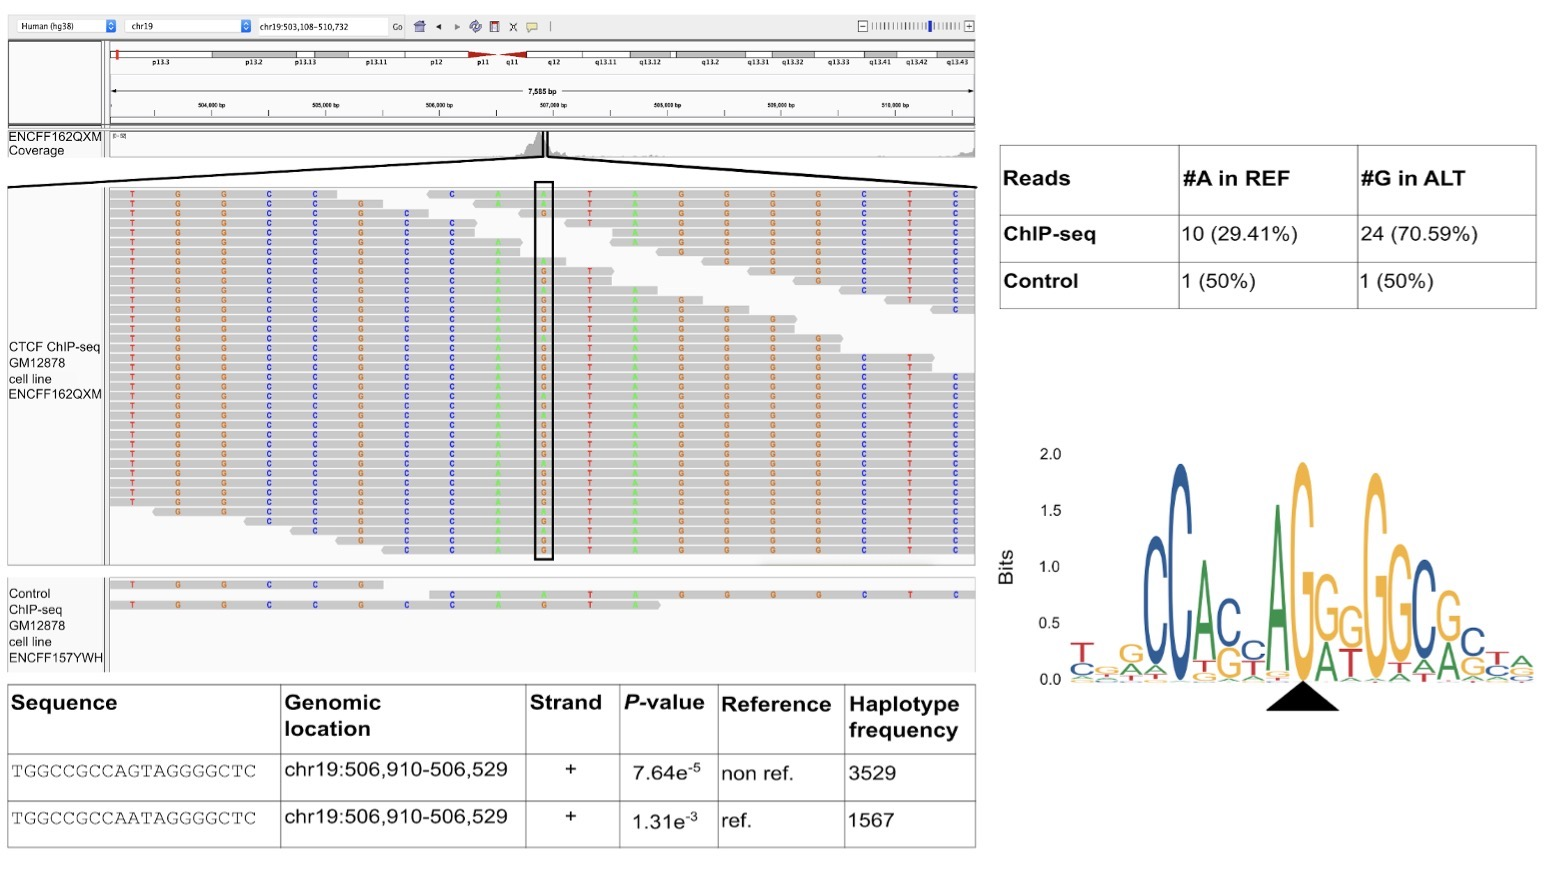
\includegraphics[width=\textwidth]{figures/grafimo2.jpg}
	\caption[Searching CTCF motif on VG with \grafimo provides an insight on how genetic variation affects putative
binding sites]{\textbf{Searching CTCF motif on VG with \grafimo provides an insight on how genetic variation affects putative
binding sites. (A)} Potential CTCF occurrences statistically significant (P-value < 1e-4) and non-significant found in the
reference and in the haplotype sequences found with \grafimo oh hg38 1000GP VG. (\textbf{B)} Statistical significance of
retrieved potential CTCF motif occurrences and frequency of the corresponding haplotypes embedded in the VG. \textbf{(C)}
Percentage of statistically significant CTCF potential binding sites found only in the reference genome or alternative
haplotypes and with modulated binding scores based on 1000GP genetic variants \textbf{(D)} Percentage of population specific and
common (shared by two or more populations) potential CTCF binding sites present on individual haplotypes.}
	\label{fig:grafimo2}
\end{figure} 
\begin{figure}
	\centering
	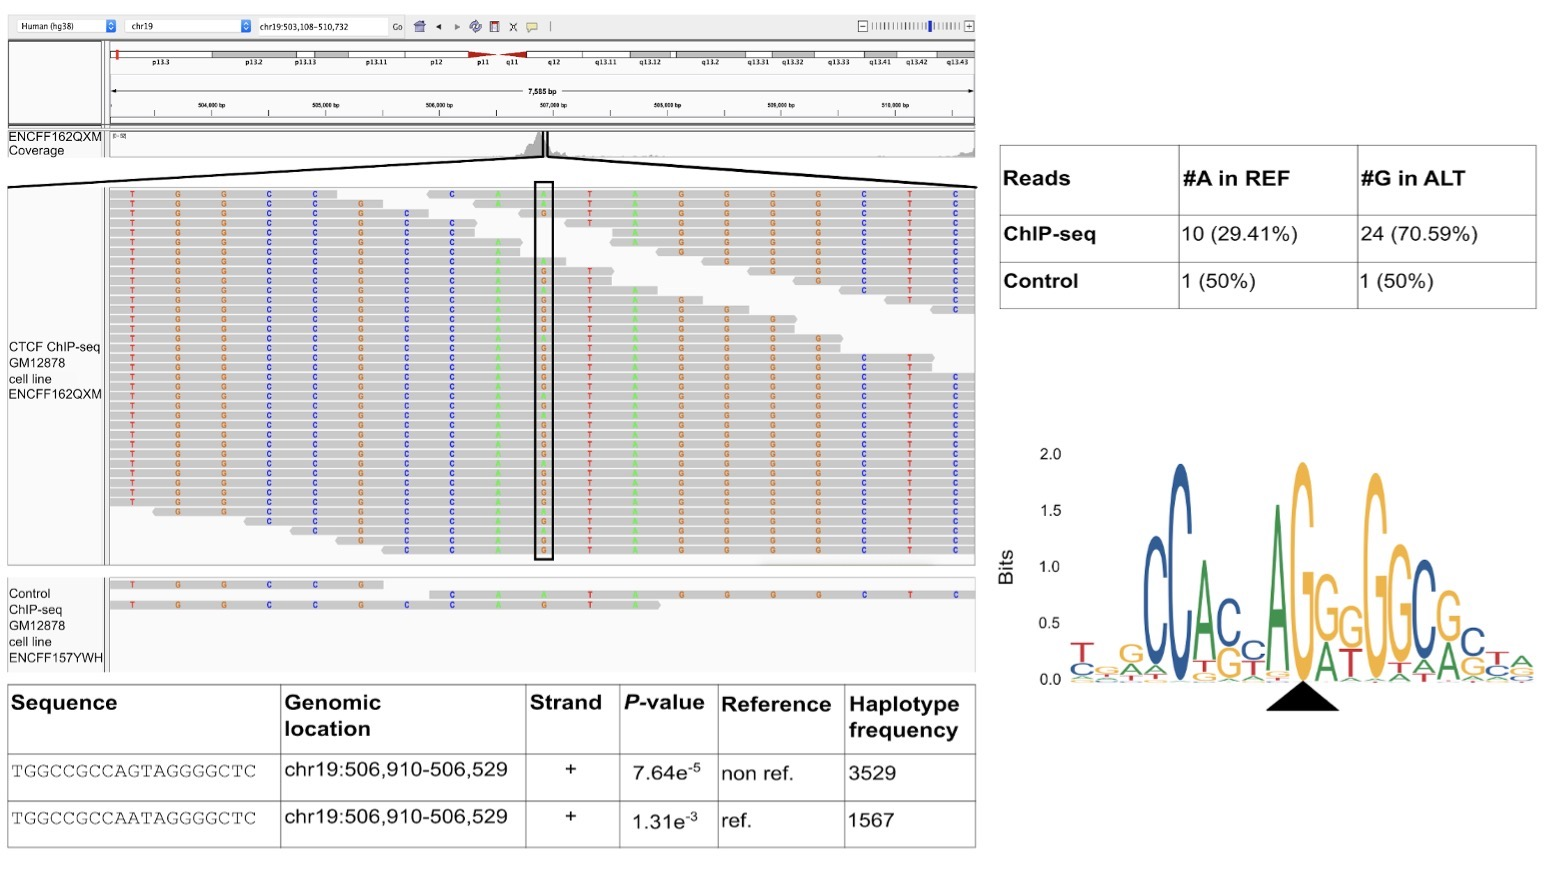
\includegraphics[width=\textwidth]{figures/grafimo3.jpg}
	\caption[Considering genomic variation, GRAFIMO captures more potential binding events]{\textbf{Considering genomic variation, GRAFIMO captures more potential binding events.} GRAFIMO reports a potential CTCF binding site at chr19:506,910-506,929 found only in haplotype sequences, searching the motif in ChIP-seq peaks called on cell line GM12878 (experiment code ENCSR000DZN). The reads used to call for ChIP-seq peaks (ENCFF162QXM) show an allelic imbalance at position 10 of the motif sequence towards the alternative allele \texttt{G}, instead of the reference allele \texttt{A}. The imbalance is captured by GRAFIMO which reports the sequence presenting \texttt{G} at position 10 (found in the haplotypes), while the potential TFBS on the reference carrying an \texttt{A} is not reported as statistically significant ($P$-value > 1e-4). CTCF motif logo shows that the \texttt{G} is the dominant nucleotide in position 10.}
	\label{fig:grafimo3}
\end{figure} 
We also found several highly significant CTCF motif occurrences in rare haplotypes that may potentially modulate gene expression in these individuals (\textbf{Fig.\ref{fig:grafimo2}(B)}). Similar behaviours were observed for ATF3 and GATA1. We also investigated the potential effects of the different length and type of mutations i.e. SNPs and indels on the CTCF, ATF3 and GATA1 binding sites. However, we did not observe a clear and general trend. By considering the genomic locations of the significant motif occurrences we next investigated how often individual TFBS may be disrupted, created or modulated. We observed that 6.13\% of the potential CTCF binding sites can be found only on non-reference haplotype sequences, 5.94\% are disrupted by variants in non-reference haplotypes and $\sim$30\% are still significant in non-reference haplotypes but with different binding scores (\textbf{Fig.\ref{fig:grafimo2}(C)}). Similar results were observed for ATF3 and GATA1. Interestingly, we observed that a large fraction of putative binding sites recovered only on individual haplotypes are population specific. For CTCF we found that 24.66\%, 6.74\%, 5.68\%, 13.01\%, 12.52\% of potential CTCF TFBS retrieved on individual haplotype sequences only are specific for AFR, EUR, AMR, SAS and EAS populations, respectively (\textbf{Fig.\ref{fig:grafimo2}(D)}).Among the unique CTCF motif occurrences found only on non-reference haplotypes in CTCF ChIP-seq peaks we uncovered one TFBS (chr19:506,910–506,929) that clearly illustrates the danger of only using reference genomes for motif scanning. Within this region we recovered a heterozygous SNP that overlaps (position 10 of the CTCF matrix) and significantly modulates the binding affinity of this TFBS. In fact, by inspecting the ChIP-seq reads (experiment ENCSR000DZN, GM12878 cell line), we observed a clear allelic imbalance towards the alternative allele G (70.59\% of reads) with respect to the reference allele A (29.41\% of reads). This allelic imbalance is not observed in the reads used as control (experiment code ENCSR000EYX) (\textbf{Fig.\ref{fig:grafimo3}}). Taken together these results highlight the importance of considering non-reference genomes when searching for potential TFBS or to characterize their potential activity in a population of individuals. We also compared the performance of GRAFIMO against FIMO. FIMO is faster and requires less memory, when scanning a single linear genome. However, when considering the 2548 individual genomes and their genetic variation, GRAFIMO proves to be generally faster than FIMO. Moreover, we benchmarked how GRAFIMO running time and memory usage change using an increasing number of threads.  By increasing the number of threads, we observed a dramatical drop in running time, while memory usage remained similar.
% ---- MotifRaptor2
\section{\motifraptor2}
Several studies have reported that genetic variants can enhance or disrupt TF-DNA binding affinity \citep{de2006regulatory, weinhold2014genome, wienert2015editing}. Genome-wide association studies (GWASs) have uncovered thousands of genetic variants (SNPs) associated with complex traits or human disease \citep{buniello2019nhgri}. Despite these efforts, functional studies to prioritize potential causal variants have lagged behind \citep{gallagher2018post}, resulting in a limited interpretation of the underlying pathophysiology mechanisms connecting variant to phenotype. A few missense SNPs can alter the function of a given TF by affecting its coding sequence, protein structure and therefore DNA binding capability, especially for Mendelian disease \citep{barrera2016survey}. For common diseases and complex traits, the great majority ($>$90\%) of associated SNPs are in non-coding regions and mainly in DNase I hypersensitive sites. These SNPs correspond to functionally relevant non-coding regions such as enhancers and promoters \citep{maurano2012systematic}. This observation suggests that chromatin state alterations and gene deregulation may be mediated by SNPs that modulate TF binding activities. In other words, genetic variants in these non-coding regions may perturb TF recognition sequences to enhance or disrupt TF-DNA binding events ultimately changing the downstream gene expression programs \citep{deplancke2016genetics}. Even if single non-coding SNPs may only moderately alter binding sites and are underpowered to explain gene expression programs, statistics on a set of SNPs modulating common TF binding sites could be significant enough to reveal the convergent regulatory mechanism in complex traits. The method we present is based on this key idea.Despite the fact that several approaches have been proposed to explore how TF binding sites could be affected by genetic variants, challenges remain. The next paragraphs provide a short summary and the rationale behind the development of Motif-Raptor. First, current availability of ChIP-seq data unfortunately limit the utility of tools such as MMARGE \citep{link2018mmarge}, GERV \citep{zeng2016gerv}, DeepSEA \citep{zhou2015predicting}, Basset \citep{kelley2016basset}, IMPACT \citep{amariuta2019impact}, RegulomeDB \citep{boyle2012annotation}, HaploReg4 \citep{ward2012haploreg}. In fact, these tools are extremely powerful and practical only when genome-wide maps of TF occupancy and/or chromatin marks in relevant cellular contexts are available. Therefore, in \citep{yao2021motif}, the authors found a unique value proposition in developing a framework to accommodate scenarios in which only PWM models and gene expression data are available. Second, available models based on ChIP-seq or PWM data do not systematically provide a global ranking and the significance of the TFs based on all trait-associated variants, rather a per SNP scoring. In fact, current methods based on PWM and/or DNase I-seq data, such as Combined Annotation Dependent Depletion (CADD, \citep{maurano2015large}), CENTIPEDE \citep{moyerbrailean2016genetics, pique2011accurate}, Affinity Testing for regulatory SNPs (atSNP, \citep{zuo2015atsnp}). do not provide a procedure to formally test the global effect of a set of GWAS variants on the set of overlapping TF binding sites. To solve this limitation, \motifraptor proposed a novel genome-wide statistic to prioritize putative causal TFs based on the entire set of binding sites and overlapping variants rather than single loci. Third, these methods do not consider linkage disequilibrium (LD) for the tagged loci by the GWAS-associated variants. This is important given that several non-causal SNPs have similar association scores as the true causal ones and that this potentially confound the analysis. In fact, these false positives can dilute our power of detecting the true mechanisms behind the causal variants. \motifraptor's approach tries to account for this problem based on the two following strategies. By relying on cell type-specific chromatin accessibility regions, it is already reducing the space of variants in each LD block. To implicitly account for local LD structure, \motifraptor samples the background set of chromatin accessibility regions in close proximity of the regions that are specific for each cell type. With these strategies, \motifraptor mitigates the problem by specifically looking for variants within regions that are cell type specific. Among available tools only SLDP (Signed LD Profile) \citep{reshef2018detecting} overcomes this problem and offers a genome-wide significance score for each TF, based on the directional modulation of TF binding sites by SNPs. Another tool, GREGOR (Genomic Regulatory Elements and Gwas Overlap algoRithm) \citep{schmidt2015gregor}, also explicitly accounts for LD structure to assess the enrichment on sentinel SNPs in arbitrary genomic regions (e.g. to prioritize cell types based on cell type specific annotations). \motifraptor addresses the above limitations of current approaches, by providing a cell type-specific TF-centric analysis with associated statistics, comprehensive reporting and visualization functionalities. This tool can facilitate the discovery and interpretation of the action of non-coding variants on key regulators of complex traits.
% -- Design and implementation
\subsection{Design and implementation}
\motifraptor pipeline consists of three main steps (\textbf{Fig.\ref{fig:motifraptor1}}). (i) TCharacterize important cell-types through the enrichment of the phenotype associated SNPs in open chromatin regions. (ii) Search TFBS whose binding potential is significantly modulated by the previously prioritized variants, in the investigated cell-types. (iii) Identify and visualize individual TF-SNP modulation events. 
\begin{figure}
	\centering
	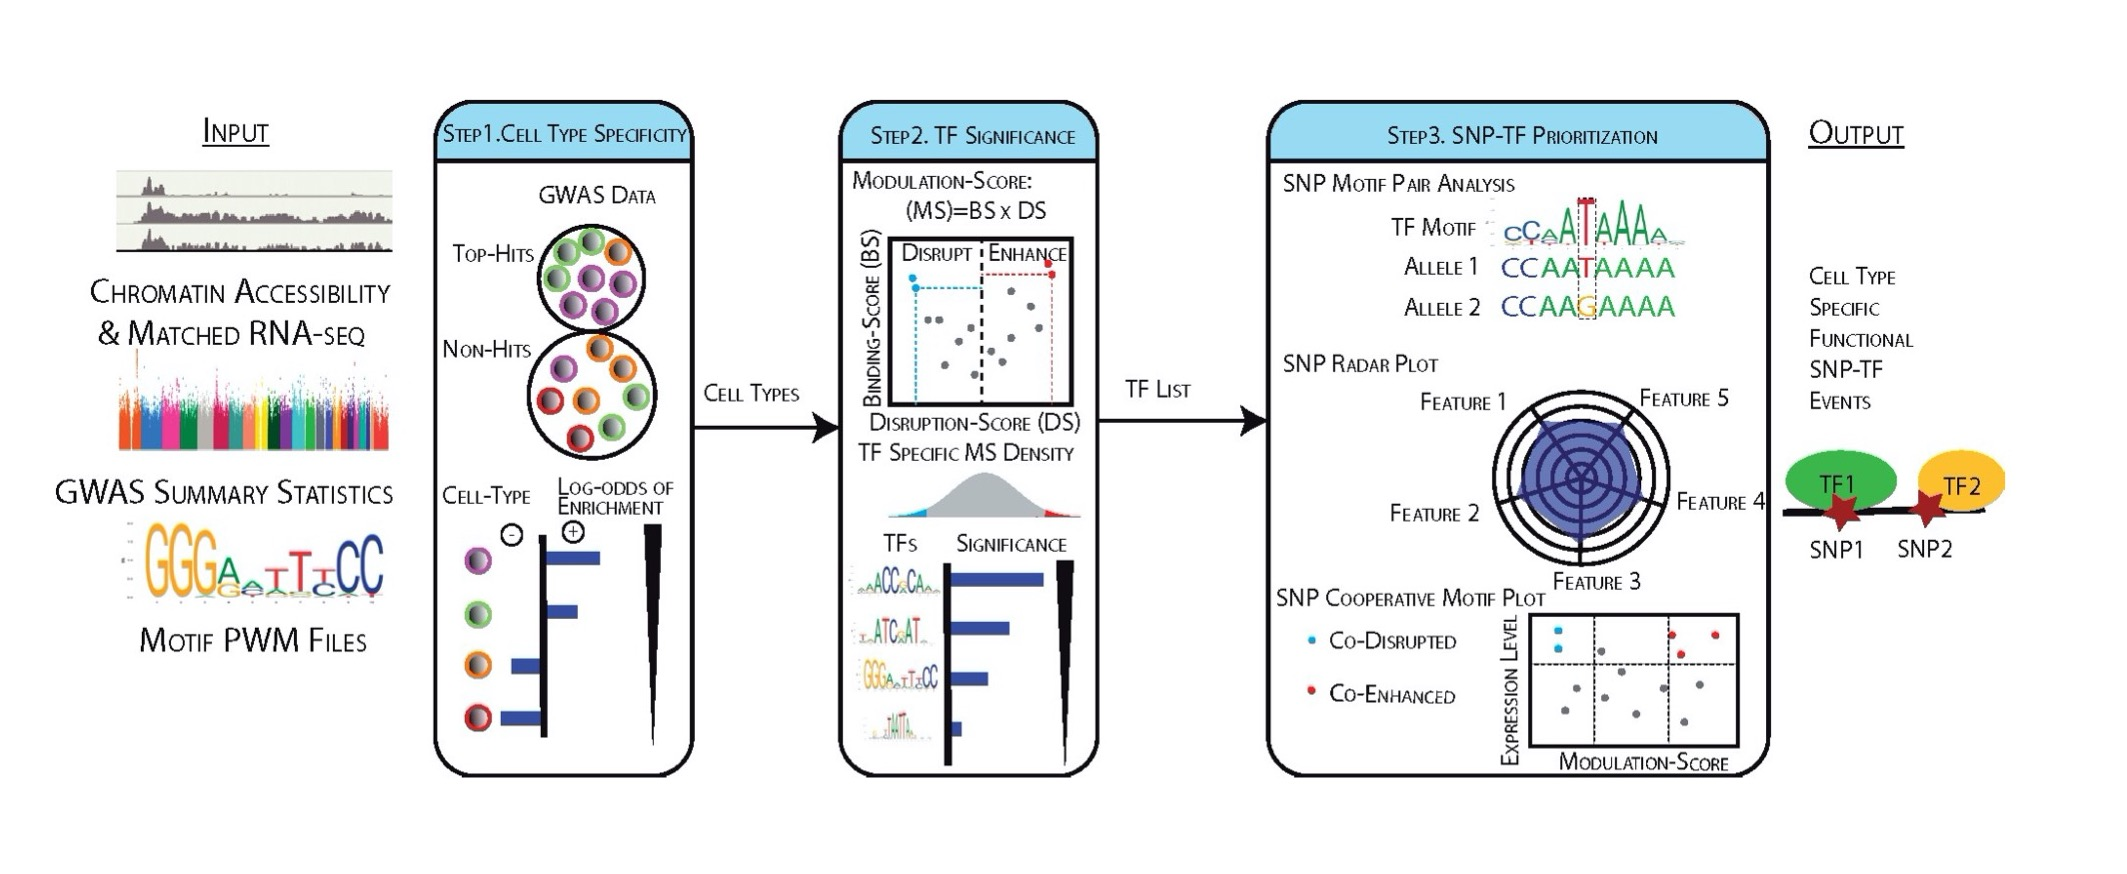
\includegraphics[width=\textwidth]{figures/motifraptor1.jpg}
	\caption[MotifRaptor analysis workflow]{\textbf{MotifRaptor analysis workflow.} Three steps are performed: (1) characterize
relevant cell types based on the enrichment of phenotype associated SNPs in chromatin accessible
sites, (2) find TFs with binding sites that are significantly modulated by genetic variants in these
cell types and (3) identify and visualize individual TF-SNP regulation events}
	\label{fig:motifraptor1}
\end{figure} 
% - Quantifying the genetic variants effects on TF binding sites
\subsubsection{Quantifying the genetic variants effects on TF binding sites}
To assess the impact of genetic variants at a certain TF binding site,, \motifraptor implements an efficient genome-wide and threshold-free scoring procedure, scanning all the binding sites overlapping the target variants. Given a genomic sequence $s$, where $|s|=m$, and a position weight matrix (PWM), the score $M(i,S_{i})$ indicates the likelihood of observing the nucleotide $S_{i}\in\{A,C,G,T\}$ at position $i$, where $1 \leq i \leq m.$ We derive the binding score $BS$ from $M(i,S_{i})$ as a log-likelihood score computed over the entire binding site and corrected to account for genome-wide nucleotide frequencies, or background frequencies, $B(s_{i})$:
\[
	BS = \log{\prod^{m}_{i=1}{\frac{M(i,s_{i})}{B(s_{i})}}} = \sum^{m}_{i=1}{(\log{M(i, s_{i}))} - \log{B(s_{i})})}
\] 
from this formulation, \motifraptor derives a disruption score $DS$, capturing the potential impact of genetic variants on a given binding site. Given a target variant, \motifraptor assumes two haplotypes, denoted by $s_{ref}$ and $s_{alt}$, for the reference and alternative alleles, respectively. \motifraptor scores each allele to obtain the binding score for the reference and alternative alleles (i.e.  $BS(s_{ref})$ and $BS(s_{alt})$). For scalability reasons it limits the computations to a region spanning 61 bp, centered around the target variant. For each region \motifraptor considers the best putative binding position $K$ for both $s_{ref}$ and $s_{alt}$:
\[
	K = \argmax_{1 \leq k \leq m}(BS(s_{ref, k:k+m-1}, M), BS(s_{alt, k:k+m-1}, M))
\]
Therefore, the disruption score at K is defined as:
\[
	DS = \Delta BS
\]
The value and sign of the $DS$ become informative indicators on the directionality and strength of the target variant impact on TF binding. In fact, positive $DS$ indicate enhanced binding affinities, while negative values a reduced binding potential. Since different TF binding site motifs have diverse length and specificities, \motifraptor rescales both the $BS$ and $DS$ in $[0,1]$ and $[-1,1]$, respectively. Given the rescaling of the two scores, \motifraptor defined a Binding-Disruption (BD) space to visualize and summarize the TF-SNP modulation events globally and across different factors.
% -- Assessing TF-SNP modulations significance
\subsubsection{Assessing TF-SNP modulations significance}
To quantify the significance of the predicted TF-SNP modulation events prioritized, \motifraptor employed a method based on the central limit theorem (CLT). Therefore,  estimated a complete null-model based on the enumeration of all potential binding sites on the genome. To maintain the scalability, \motifraptor employed advanced sequence data structures like Suffix Arrays and Longest Common Prefix Arrays. These data structures allow the exhaustive enumeration keeping the method scalability.  Given a set of target variants $T$, to assess if they significantly modulate TF binding events, \motifraptor tests whether the B-S space significantly differed from the B-S space obtained from a set of background SNPs $B$.  To assess the difference between the distributions \motifraptor uses a non-parametric test with null hypothesis $E(D_{B-S_{space}}(T))=E(D_{B-S_{space}}(B))$. Since based on the CLT, the distribution of the sample mean of $B$ converges to a normal distribution, its mean and variance are equal to $E(D_{B-S_{space}}(B))$ and $\frac{\Var(D_{B-S_{space}}(B)}{N_{samples}}$,  regardless of the underlying B-S space values distribution. Therefore, \motifraptor tests the significance of both the enhanced binding $((D_{B-S_{space}}(T)) > E(D_{B-S_{space}}(B)))$, disrupted binding $((D_{B-S_{space}}(T)) < E(D_{B-S_{space}}(B)))$, or both. This procedure combined with efficient data structures allows to identify significant genome-wide shifts in TF-SNP binding modulations without using predetermined scores or cutoff on $p$-values.
% -- Improving MotifRaptor by employing SVM-based motif models
\subsection{Improving MotifRaptor by employing SVM-based motif models}
In the case study presented in the original paper, \motifraptor's predictions were supported by literature, suggesting that it leverages promising ideas. However, \motifraptor’s main limitation is the employed computational models to represent TF binding motifs. Despite position weight matrices \citep{stormo2000dna} (PWMs) are simple, intuitive, and widely employed TF motif models, PWMs carry several drawbacks that often result in under- or over-estimation of non-coding variant impact on TFs binding landscape \citep{tognon2023survey}. TF SVM-based motif models \citep{tognon2023survey, boeva2016analysis} have been demonstrated to overperform PWMs in several tasks, such as prediction of binding events and variants impact on TF binding sequences. However, while several publicly available resources provide complete and extensive collections of motif PWMs, to our knowledge there is no complete collection of SVM-based TF motifs. Therefore, we propose an extensive and curated collection of SVM-based motifs as well as a novel approach to annotate the functional impact of non-coding variants on TF binding landscape using SVM-based models, which interpolates different omics data, such as transcriptome, DNase-seq \citep{john2011chromatin}, ATAC-seq \citep{buenrostro2013transposition}, etc. 
% - Building a library of transcription factor SVM-based models
\subsubsection{Building a library of transcription factor SVM-based models}
SVM-based models have demonstrated superior performance compared to traditional PWMs \citep{tognon2023survey}. However, a significant drawback persists as no motif database currently offers these advanced SVM-based models. Moreover, the interpretability of these models remains a challenging issue, and there is a scarcity of motif analysis tools that harness the power of SVMs-based motif models. To address these limitations,  we propose the creation of a comprehensive library comprising SVM-based motif models. To compute the SVM-based motif models we use ChIP-seq data from ENCODE \citep{encode2012integrated}.  To enhance model reproducibility, we modified FactorBook's model computation pipeline \citep{pratt2022factorbook} (\textbf{Fig.\ref{fig:motifraptor3}}).
\begin{figure}
	\centering
	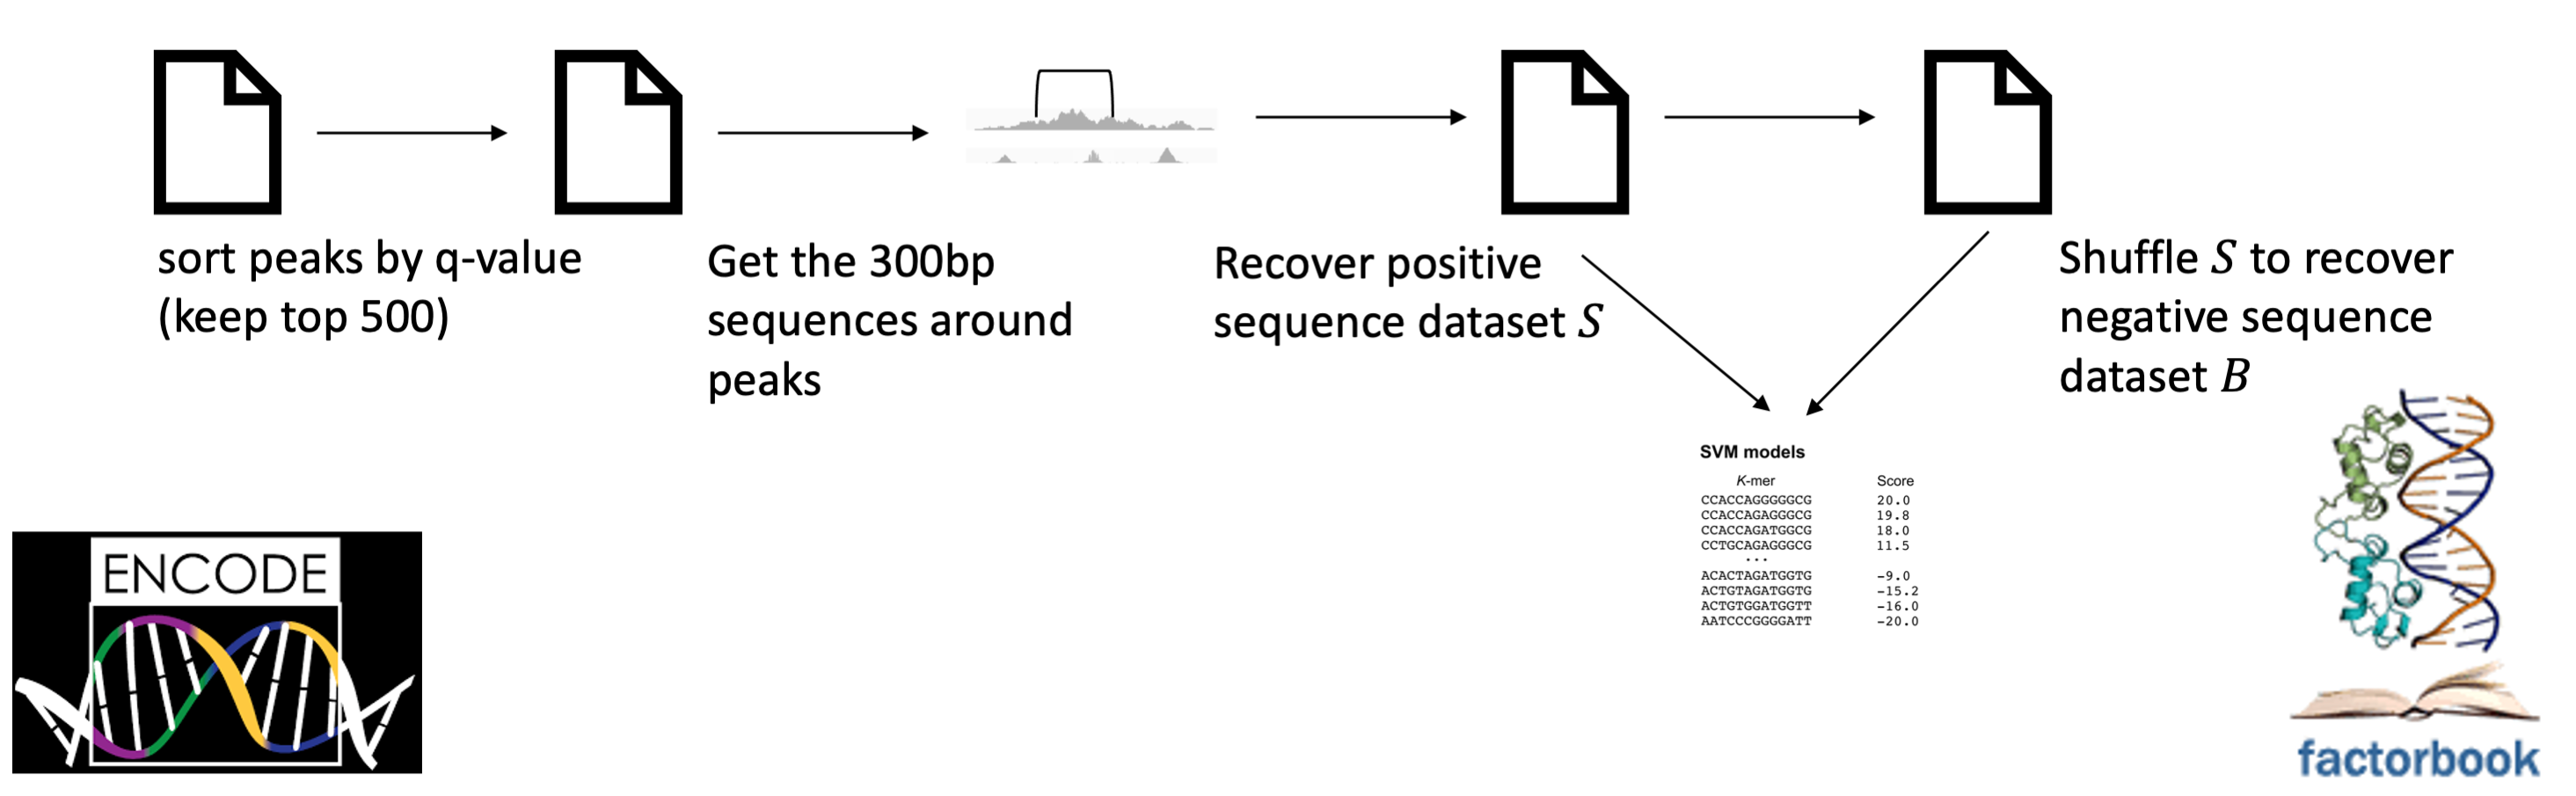
\includegraphics[width=\textwidth]{figures/motifraptor3.png}
	\caption[SVM-based motif models computation workflow]{\textbf{SVM-based motif models computation workflow.} For the sake of reproducibility, we follow the model computation pipeline employed by FactorBook database, to derive PWM models from ENCODE data.}
	\label{fig:motifraptor3}
\end{figure} 
To compute the models we selected ChIP-seq peaks datasets from ENCODE retrieved on different tissues and cell types.  For each ChIP-seq dataset, we selected the top 500 peak sequences sorted by $q$-value. Then, we shrinked the surviving peaks to 300 bp centered around the peak signal center. After recovering the resulting genomic sequences, we constructed a background dataset by shuffling the original sequences. The two dataset are, then, used as input to compute the SVM models using LS-GKM \citep{lee2016ls}.
% - Comparing SVM-based and PWM motif models predictive power
\subsubsection{Comparing SVM-based and PWM motif models predictive power}
\begin{figure}
	\centering
	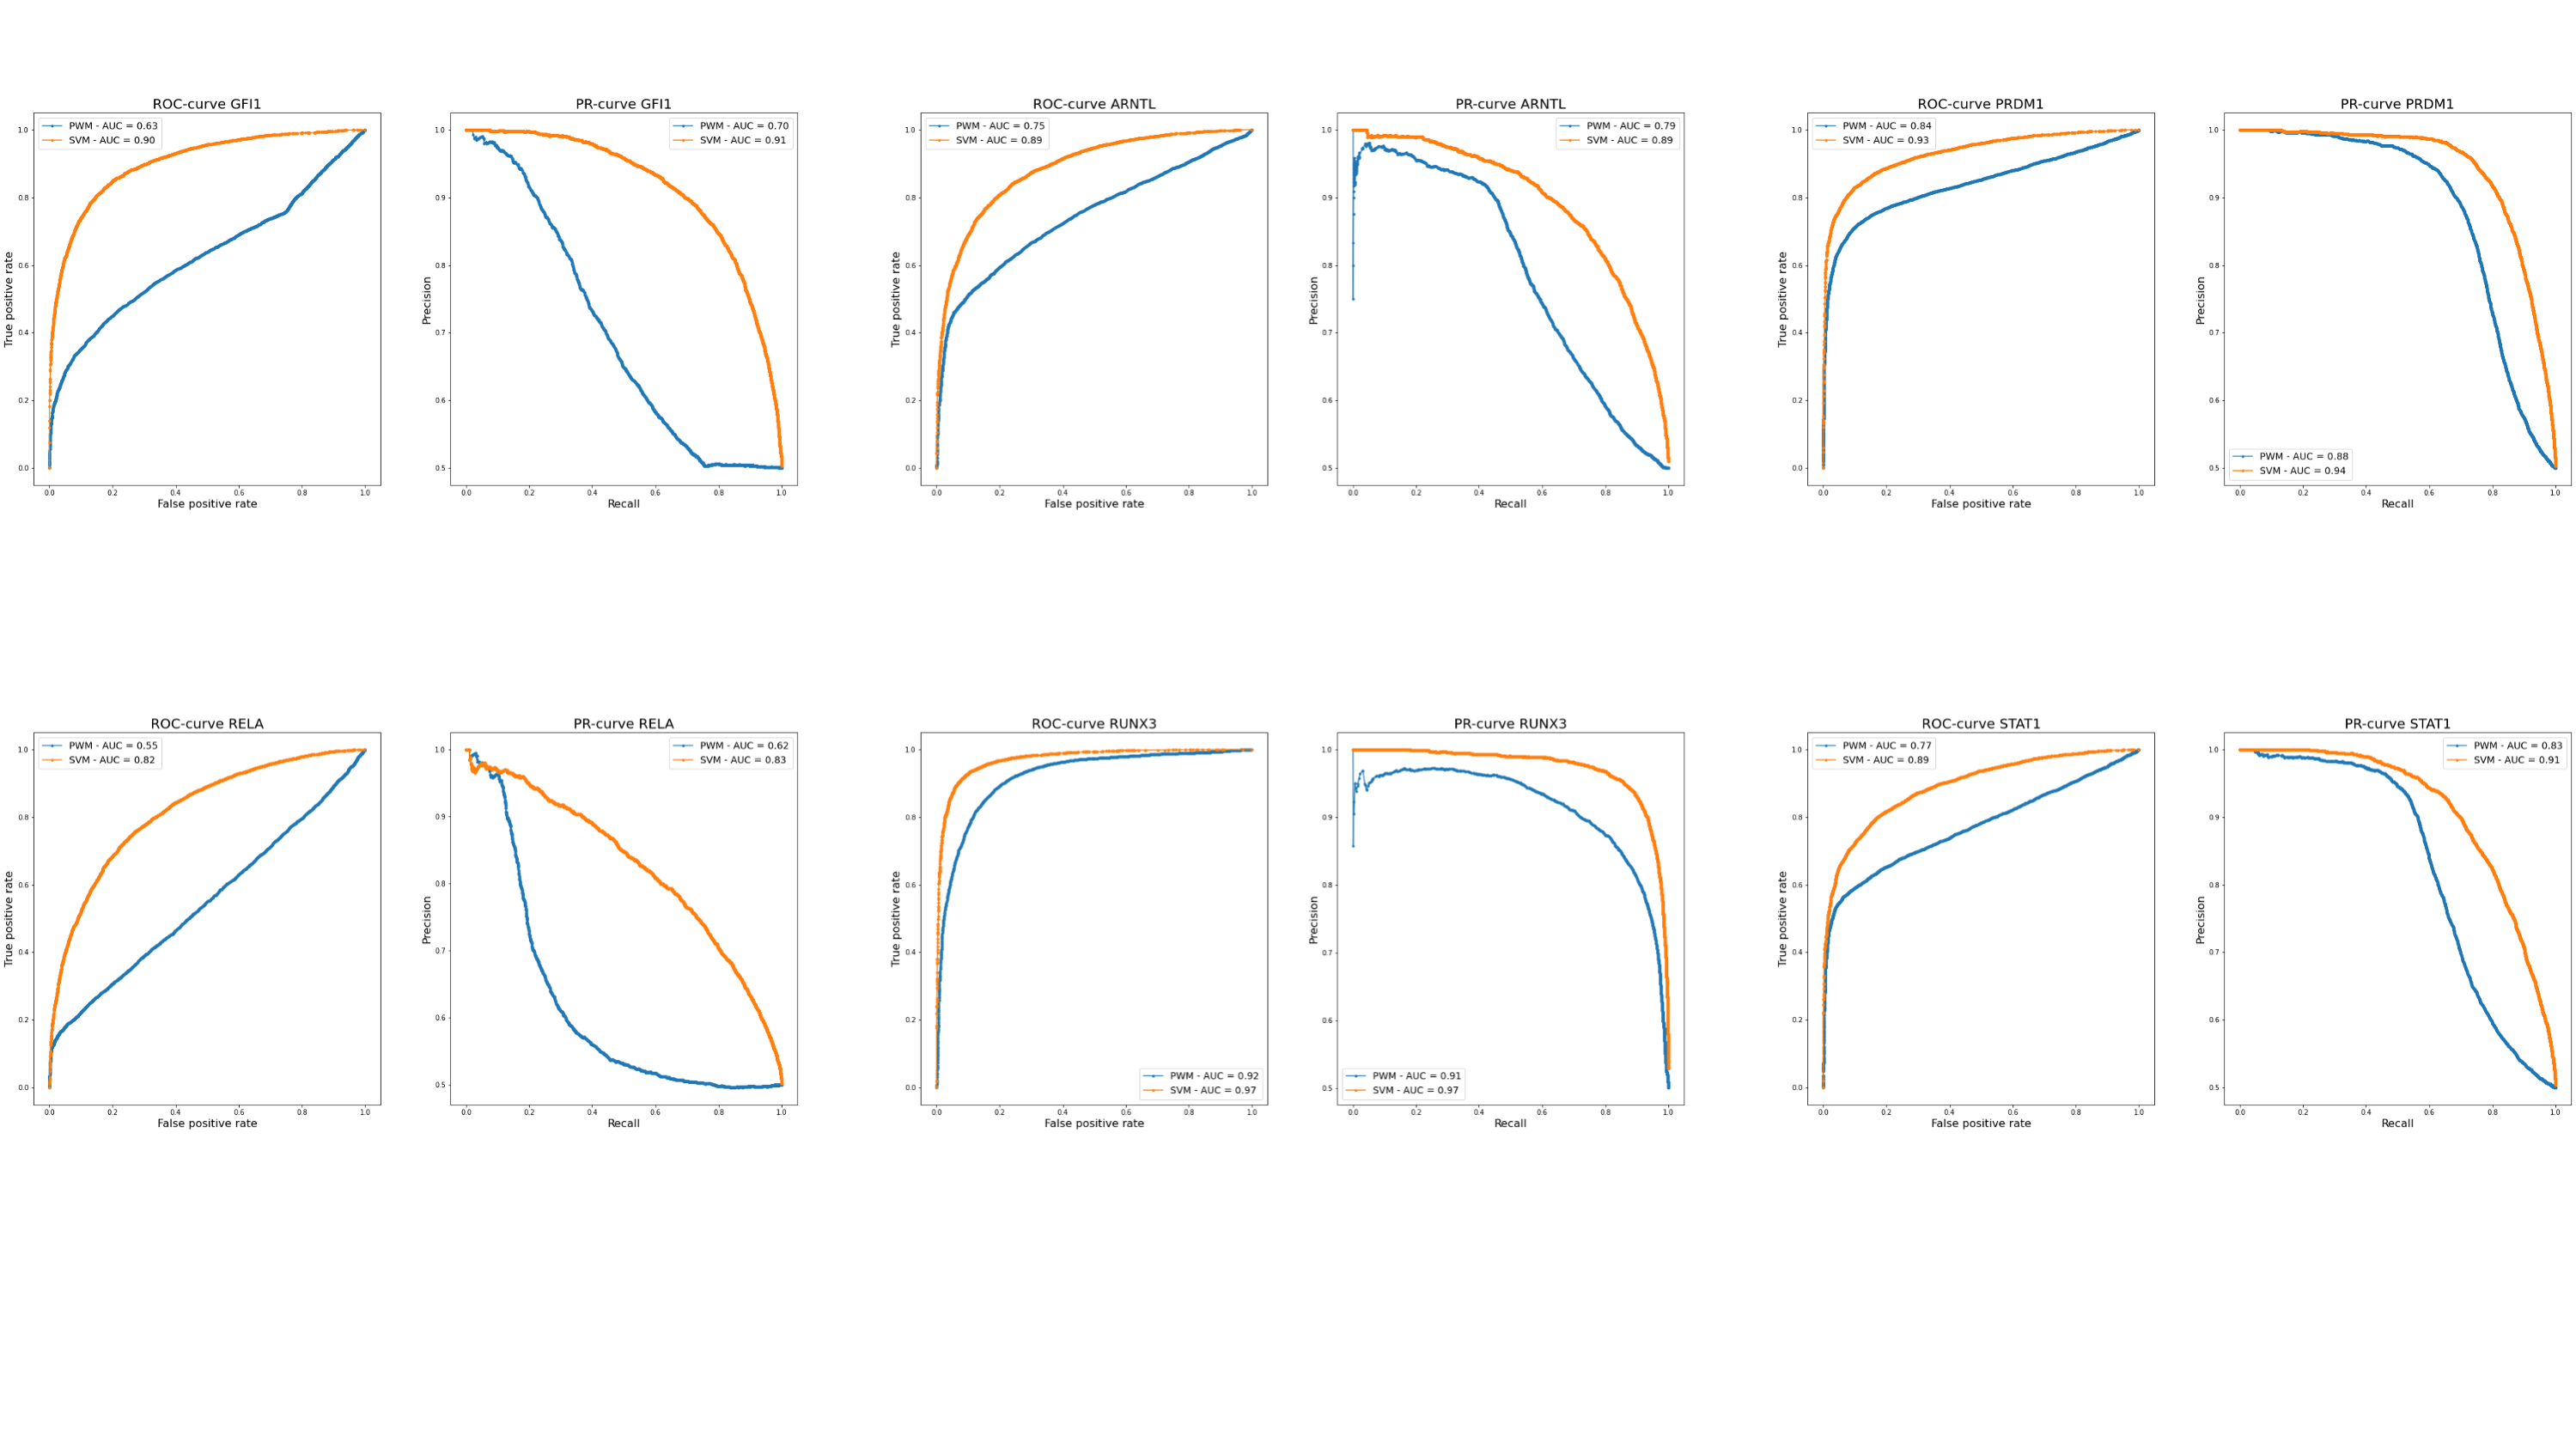
\includegraphics[width=\textwidth]{figures/motifraptor2.png}
	\caption[Comparing SVM-based and PWM motif models predictive power]{\textbf{Comparing SVM-based and PWM motif models predictive power.} We compared the predictive power of SVM-based and PWM motif models for six transcription factors: ARNTL, GFI1, PRDM1, RELA, RUNX3 and STAT1. Both models were trained on ENCODE ChIP-seq data (cell line GM12878). To train SVM-based models we followed the described pipeline, while to train PWM models we replaced LS-GKM with MEME. The predictive perfomance of the two models have been compared computing ROC- and PR-curves.}
	\label{fig:motifraptor2}
\end{figure} 
We demonstrate the improvements brought by SVM-based motif models over PWMs, by comparing the predictive power of the two models in terms of ROC- and PR-curves. For this analysis we selected the six TFs that have been previously identified in the original \motifraptor publication to be affected by mutations linked to rheumatoid arthritis: ARNTL, GFI1, PRDM1, RELA, RUNX3, and STAT1. For the assessment we employed the original and the modified FactorBook pipeline, where the latter replaces MEME with LS-GKM to compute the SVM models. MEME \citep{bailey1994fitting} is a widely used software to compute PWM motif models from sequence data. To train and test the models we selected one ChIP-seq dataset for each TF (GM12878 cell line) from the ENCODE data portal. After training, we compared models' performance via a $4$-fold cross-validation (75\% training and 25\% testing) on the top 500 peaks, selected following FactorBook's pipeline. By running our comparison, we observed that generally SVM-base motif models better predict binding events than PWMs, in both terms of ROC and PR-curves (\textbf{Fig.\ref{fig:motifraptor2}}).
% -- Future directions
\subsection{Future directions}
In the next future we plan to complete our SVM-based motif models catalog extending the presented analysis to all the remaining TFs whose ChIP-seq data are available in ENCODE. Additionally, ENCODE datasets could be integrated employing datatasets from different databases, such as Cistrome \citep{zheng2019cistrome} or GTRD \citep{kolmykov2021gtrd}. Moreover, we plan to release to the community the complete SVM motif models catalog. We also plan to train models on SELEX data rather than ChIP-seq and compare the resulting models. Importantly, since SELEX is a method less susceptible to noise than ChIP-seq the resulting models could potentially provide an even larger boost of models' predictive performance. We plan to modify \motifraptor scanning algorithm for both PWM and SVM motif models to consider haplotypes, and indels. In fact,  currently \motifraptor consider only SNP and treats them as independent events, however it is known that complex SNP-SNP, SNP-indel, indel-indel combination can happen \citep{tognon2021grafimo}, often with signifcant effects on TF binding potential.
% ------ CRISPR off-targets
\mychapter{6}{CRISPR genome editing}
CRISPR genome editing \citep{cong2013multiplex} has revolutionized genetic engineering, allowing for precise modifications in the genomes of living organisms. CRISPR offers a versatile and programmable approach, linking coupling binding to genomic target sequences with diverse effector proteins, restricted by protospacer adjacent motif (PAM) sequences.  By delivering the Cas9 nuclease complex coupled with a synthtic guide RNA (gRNA), into a cell CRISPR provides a simple and programmable means to modify genomic sequences at specific locations, enabling the addition or removal of genes \emph{in vivo}. Significantly, CRISPR opens up unprecedented opportunities for developing novel therapies by introducing precise genetic or epigenetic modifications to targeted genomic regions. The precision of CRISPR-Cas9 editing hinges on two crucial factors: (i) the target sequence, a 20 bp string within each CRISPR locus of the gRNA array \citep{ran2013genome}, which typically has multiple unique targets, and (ii) the PAM sequence, short nonspecific sequences scattered throughout the genome \citep{ran2013genome}, which Cas9 identifies to initiate editing. Once the requisite sequences are assembled, Cas9 locates its target on the genome under the guidance of the gRNA. The Cas9 nuclease opens both strands of the genomic target, to introduce novel and precise modifications. Cas9 operates primarily through two mechanisms: (i) knock-in and (ii) knock-out mutations,(\textbf{Figure \ref{fig:crispr}}). In knock-in, homology-directed repair (HDR) employs DNA sequences that resemble the target to mend the Cas9-induced breaks in the genome, using exogenous DNA as a template for repair. It is essential to note that this method relies on specific and isolated damaged sites within the target region to initiate DNA repair processes. Conversely, in knock-out, the mutations in the DNA introduced by Cas9 result in the repair of breaks via nonhomologous end joining (NHEJ). Repair through NHEJ often leads to random insertions and deletions in the target sequence, which can disrupt, enhance, or alter the function of the targeted site.
\begin{figure}
	\centering
	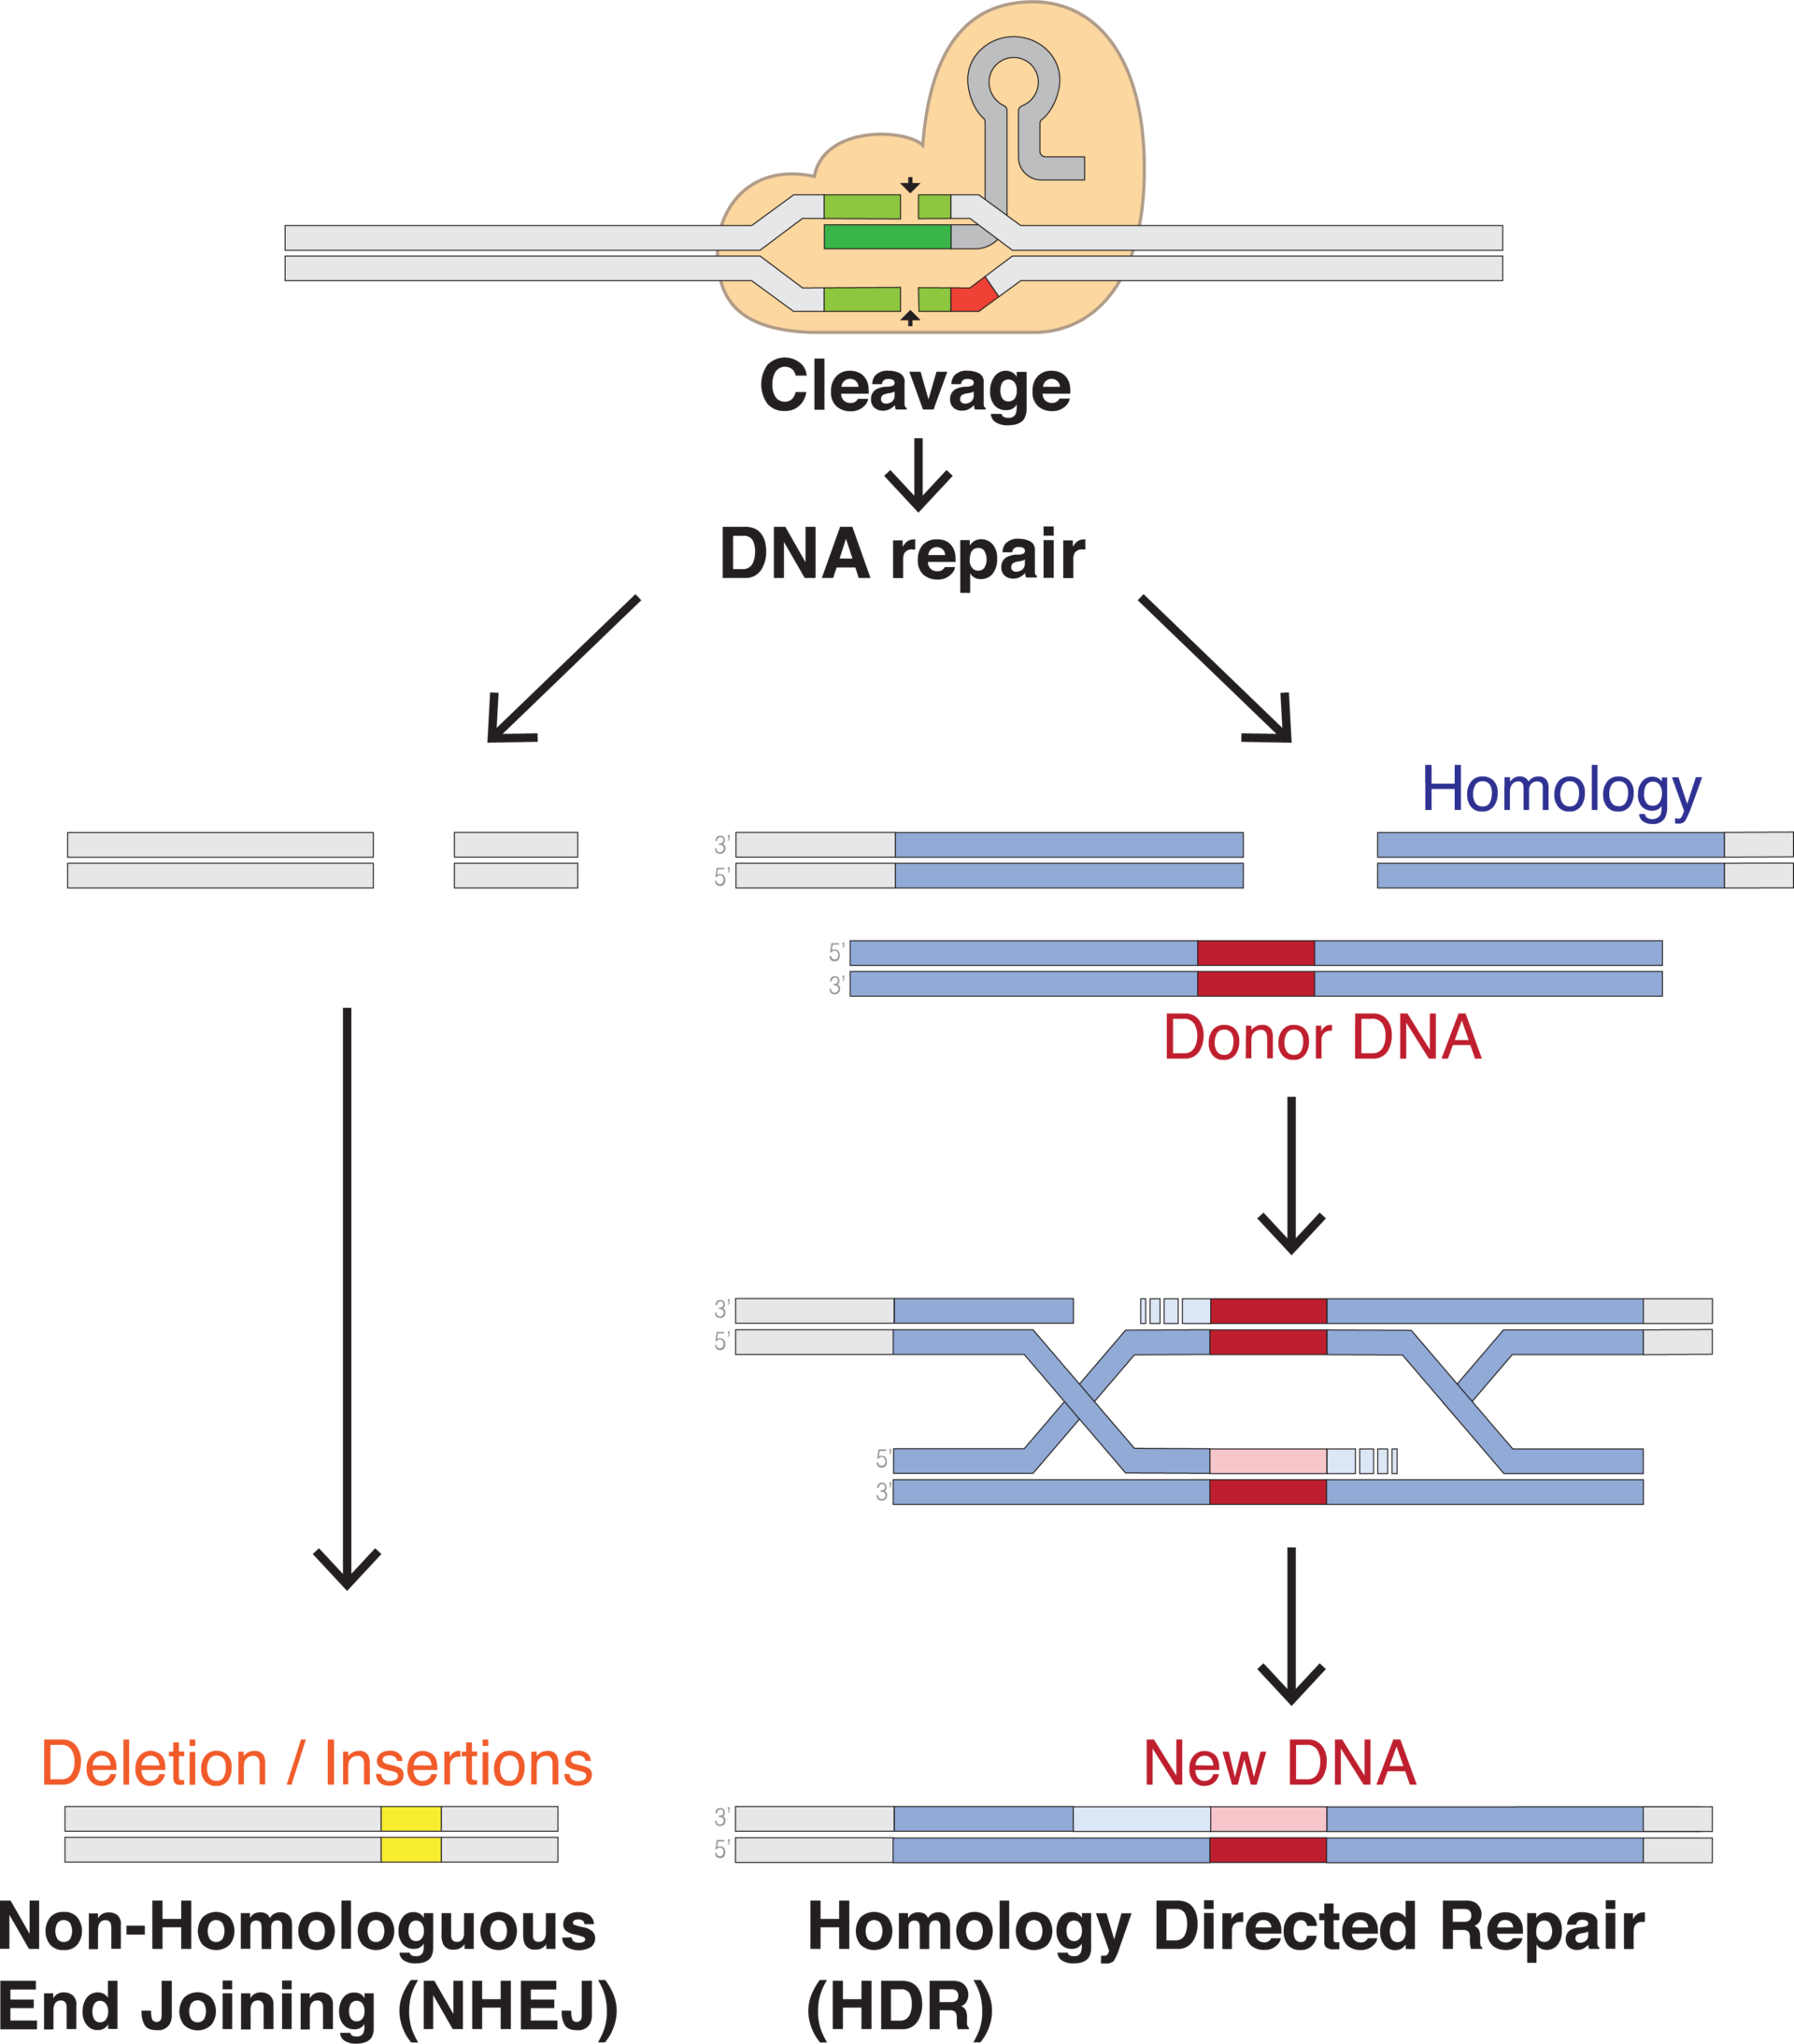
\includegraphics[width=\textwidth]{figures/crispr.png}
	\caption[CRISPR gene editing via HDR and NHEJ]{\textbf{CRISPR gene editing via HDR and NHEJ.}}
	\label{fig:crispr}
\end{figure} 
Given that CRISPR-Cas9 empowers precise yet potentially random gene disruption, the meticulous design of guide RNAs (gRNA) to effectively steer Cas9 toward the intended target sequence (\emph{on-targets}) is of paramount importance. This precision is essential to prevent unintended and potentially hazardous alterations in non-targeted sequences (\emph{off-targets}). Moreover, genetic variants can potentially modify target and PAM sequences, thereby impacting both on-target and off-target potentials. Consequently, when crafting gRNA designs, it becomes imperative to account for genetic diversity, particularly in clinical settings, in order to avert possible undesired and hazardous consequences within the host genome.
% ---- Benchmarking whole genome sequencing to detect CRISPR genome editing events
\section{Benchmarking whole genome sequencing to detect CRISPR genome editing events}
One of the major hurtles for the clinical adoption of CRISPR genome editing technologies is the risk of genome editing at unpredicted genomic sites \citep{fu2013high}. Computational and experimental strategies have been developed to nominate off-target editing sites \citep{clement2020technologies}. ). In practice, these nomination strategies produce a ranked list of sites, of which the top hits are prioritized for validation using amplicon sequencing to quantify evidence of genome editing\citep{akcakaya2018vivo}. However, nomination strategies have an arbitrary cutoff or no cutoff to distinguish which sites should be experimentally validated, and the number of sites chosen for validation are sometimes selected subjectively based on budget or choosing nice round numbers (e.g. the top 100). Unfortunately, the possibility of editing at nominated sites lower down the prioritized list-combined with the possibility that the nomination strategies may not comprehensively capture the genome editing dynamics of actual CRISPR genome editing–have led many to suggest that reliance on nomination strategies may be insufficient to exclude editing at unpredicted sites.  Whole-genome sequencing (WGS) has been proposed as a standard to comprehensively examine the genome for evidence of genome editing. WGS has several benefits, including the ability to potentially measure genome editing activity at every base in the genome, and to measure complex genome editing outcomes such as translocations. However, despite increased availability and reduced cost of genome sequencing, WGS remains an expensive proposition as significant sequencing of the entire genome must be performed to detect rare editing events, and it is difficult to distinguish rare editing events from sequencing errors. WGS has been used to detect genome editing events in clonal cell lines \citep{smith2014whole, veres2014low} where individual cells within a clone serve as replicates to reduce bias of sequencing artifacts. However, this method is inadequate for use in detecting rare off-targets because the limit of detection is based on the number of clones (e.g. WGS of 100 clonal lines would need to be performed to detect an editing event at a 1/100 (1\%) rate). 
To investigate the utility of WGS as a method to detect genome editing events genome-wide in bulk populations, we have created models for the sequencing depth required for detection of editing events. We have produced ultra-deep 1000x WGS datasets of genome-edited samples and used them to characterize editing at on- and off-target sites, and compare editing detection in WGS to several experimental nomination and computational detection methods. We then propose an unbiased genome editing detection method which can identify the genome editing from WGS data in cases when the CRISPR guide sequence is not known. Together, these models, datasets, and methods provide an assessment of the utility for whole genome sequencing in the detection of genome editing. 
% -- Modeling sequencing depth requirements to detect genome editing
\subsection{Modeling sequencing depth requirements to detect genome editing}
The actual problem of detecting genome editing can be broken into two parts: (i) sequencing genomic DNA with sufficient depth to detect editing at a given site, and (ii) correctly interpreting the sequencing data (e.g. read alignment and variant calling) to discriminate true CRISPR edits from technical noise. We address the first question regarding sequencing depth using a binomial model, and use simulated samples to measure the ability of existing mutation callers to detect edited genome-edited reads as such.
DNA sequencing for the detection of editing events can be performed in a heterogenous population of edited cells with a detection limit and detection power proportional to the sequencing depth. This approach to determining sequencing depth requirements applies to amplicon sequencing of a single locus as well as to whole-genome sequencing. We note that WGS can be performed at low coverage on clonal lines to detect genome editing in single cells, but in this case the limit of detection is defined based on the number of single cell clones that can be sequenced. To detect genome editing – especially rare editing events – in cell populations, samples must be sequenced with sufficient depth, meaning that the sequence of sufficiently many DNA molecules must be read in order to find one containing an editing event. To measure rarer editing events, deeper sequencing must be performed. We used a statistical model to formalize the power to recover editing events at varying frequencies based on the binomial distribution \citep{petrackova2019standardization}. Using this model we can calculate the sequencing depth required to observe a certain number of reads given a frequency of edited reads in a sample. For example, 30 reads are required to detect a single edited read in a sample with a mutation rate of 10\% and 300 reads are required to detect a single edited read in a sample with a mutation rate of 1\% at 95\% power, or that in 95\%. We can also use the binomial distribution confidence interval to calculate the range of true editing rates given an observed editing rate and sequencing depth. For example, the 95\% confidence interval for an edit in 15/30 reads is between 31.3\% and 68.7\%. In order to assess the ability of mutation callers to detect genome editing events, we created simulated samples by inserting mutations found in reads from amplicon sequencing of 14 on- and off-targets from Fu \emph{et al}. \citep{fu2014improving} into whole-genome sequence from the Genome in a Bottle Consortium \citep{zook2016extensive}. We plan to measure the ability of three commonly-used mutation callers to recover simulated reads resulting from genome editing \citep{mckenna2010genome, kim2018strelka2, koboldt2012varscan}.
% -- Generation of WGS datasets
\subsection{Generation of WGS datasets}
Whole-genome sequencing is commonly performed to identify mutations genome-wide, and has been applied in clinical settings to detect disease-associated germline mutations \citep{thiffault2019clinical}. Clinical whole-genome sequencing aims for 30x-50x coverage of samples, and 40x coverage has been reported to provide sufficient depth to detect heterozygous and homozygous SNPs \citep{sun2021characterizing}. According to our model introduced above, sequencing at 30x can detect one edited read in the context of approximately 5\% genome editing at 80\%. In order to detect rarer editing events, deeper sequencing must be performed. We aimed to create whole genome sequencing libraries at 1000x, which should be able to detect one edited read with a 0.2\% editing rate with 80\% power.  We performed genome editing in K562 and GM12878-Cas9 cell lines \citep{ma2017crispr} with four guides with varying specificities as measured by the number of sites in the genome with sequence homology with up to 4 mismatches. We selected RNF2 (precise guide, 7 off-by-4 sites), EMX1 (mid specificity, 293 off-by-4 sites), HEKSite4 (mid specificity, 832 off-by-4 sites), and VEGFASite3 (promiscuous, 6509 off-by-4 sites). Additionally we used a Cas-12a guide targeting DNMT1Site3 as a control guide. For each sample we prepared PCR-free sequencing libraries. Genomic sequencing depth was measured using Mosdepth \citep{pedersen2018mosdepth}, and showed a minimum of 89\% genomic coverage at 1000x in GM12878 and at least 57\% genomic coverage at 1000x in K562.
% -- Measurement of editing using existing tools
\subsection{Measurement of editing using existing tools}
We used our WGS samples to test the ability to identify edited bases by existing tools which are used for variant calling in non-CRISPR settings. Although these tools have been developed to disregard technical artifacts such as sequencing errors, and some have been developed to detect rare alleles, none have been developed to identify CRISPR-edited reads or genomic sites of CRISPR editing. We therefore tested the ability of these tools to detect CRISPR editing at and around sites nominated by experimental (GUIDE-seq \citep{tsai2015guide}, CIRCLE-seq \citep{tsai2017circle}), and computational (Casoffinder \citep{bae2014cas}) methods.  For each nominated region, we defined a region within 100bp of the predicted cutting location where we would expect to see CRISPR editing. We also defined 10Kb windows up- and downstream from the nominated region (not including the 100bp window) where we did not expect to see editing. We used Mutect \citep{mckenna2010genome}, Varscan \citep{koboldt2012varscan},  and Strelka \citep{kim2018strelka2} were used to identify variants for each nominated region, and classified variants within the 100bp window as true-positives and variants in the 10kb flanking windows as false-positives. 
% -- Enhancement of off-target editing detection by predictive models
\subsection{Enhancement of off-target editing detection by predictive models}
Our WGS dataset provides the benefit of being able to investigate editing across the genome without knowing beforehand the sites to be investigated – albeit at a depth of around 1000x coverage. This is in contrast to strategies such as amplicon sequencing where much greater depth can be achieved but the genomic sites to be amplified must be selected in advance, and editing cannot be investigated outside the selected regions. We have capitalized on this characteristic of our WGS dataset and identify nuclease effects at a variety of regions. We used Casoffinder to identify all putative cut sites with up to 4 mismatches and 1 bulge with respect to the guide sequence, and used CRISPRessoWGS \citep{clement2019crispresso2} to calculate the percentage of reads with indels in the treated and control sample.
% -- Unbiased detection of genome editing targets
\subsection{Unbiased detection of genome editing targets}
Next, we sought to identify sites of genome editing, but without relying on knowing the sgRNA sequence used to edit the sample. This unbiased approach is valuable because it allows detection of CRISPR edits in a sample where the sgRNA was not known, and it can also be used to find CRISPR edits that may occur at locations without sequence similarity to the sgRNA. We note that many experimental nomination methods constrain reported hits to sites with homology to the sgRNA sequence because naturally occurring double-strand breaks frequently occur at fragile or AT-rich genomic sites \citep{nobles2019iguide}, ), so an unbiased method using WGS could identify guide sequence-independent editing events.  Unfortunately, WGS data contains noise from different sources that makes it difficult to identify genome editing. These sources of noise include sequencing errors, alignment errors, and allelic diversity. We developed an unbiased genome editing discovery algorithm that attempts to discriminate between sites of CRISPR editing and noise by comparing a treated sample to a control sample because we expect that these sources of noise will affect the control sample as well as the treated sample. In addition, we exploit two additional characteristics of genome editing: High rates of insertions/deletions at the on-target and diversity of editing at the on-target – we expect that more than one allele will be produced as the result of stochastic double-strand break repair after Cas9 editing. We ran our unbiased algorithm to detect ranked sites of editing in all WGS samples. The ranking of sites with putative editing correlates well between the GM12878 and K562 cell lines, suggesting that the majority of editing is reproducible across cell types. We observe slightly more sensitivity in the K562 line for detecting off-target sites nominated by CIRCLE-seq. This is likely be due to the higher editing rates in the K562 cell line. Importantly, our unbiased algorithm identifies the on-target edit site among the top hits in all guides and in both cell lines.
% ---- CRISPRme
\section{\crisprme}
CRISPR genome editing offers extraordinary opportunities to develop novel therapeutics by introducing targeted genetic or epigenetic modifications to genomic regions of interest. Briefly, CRISPR provides a simple and programmable platform that couples binding to a genomic target sequence of choice with diverse effector proteins through RNA:DNA (spacer:protospacer) complementary sequence interactions mediated by a gRNA spacer sequence matching a genomic protospacer sequence restricted by PAM sequences. Editing effectors may consist of nucleases to introduce targeted double strand breaks leading to short insertions/deletions (indels) and templated repairs (for example, Cas9), deaminases for precise substitutions (base editors) or chromatin regulators for transcriptional interference or activation (CRISPRi/a), among others, to achieve a range of desired biological outcomes \citep{anzalone2020genome}. CRISPR-based systems may create unintended off-target modifications posing potential genotoxicity for therapeutic use. Several experimental assays and computational methods are available to uncover or forecast these off-targets \citep{clement2020technologies}. Off-target sites are partially predictable based on homology to the spacer and PAM sequence. Beyond the number of mismatches or bulges, a variety of sequence features, like position of mismatch or bulge with respect to PAM or specific base changes, contribute to off-target potential \citep{clement2020technologies, bao2021tools, hsu2013dna, doench2016optimized}. Computational models can complement experimental approaches to off-target nomination in several respects: to triage gRNAs before experiments by predicting the number and cleavage potential of off-target sites and to prioritize target sites for experimental scrutiny. Genetic variants may alter protospacer and PAM sequences and therefore may influence both on-target and off-target potential. Gene editing strategies designed to specifically recognize patient mutations may increase the likelihood of editing mutant alleles, whereas variants that reduce homology to the anticipated target may decrease the efficiency of the desired genetic modification. Although a variety of in vitro and cell-based experimental methods can be used to empirically nominate off-target sites, these methods either use homology to the reference genome as a criterion to define the search space and/or use a limited set of human donor genomes to evaluate off-target potential \citep{bao2021tools, chaudhari2020evaluation}. Therefore, computational methods may be especially useful to predict the impact of off-target sequences not found in reference genomes. Prior studies considering gRNAs targeting therapeutically relevant genes using population-based variant databases like the 1000 Genomes Project (1000 G) and the Exome Aggregation Consortium have highlighted how genetic variants can substantially alter the off-target landscape by creating novel and personal off-target sites not present in a single reference genome \citep{lessard2017human, scott2017implications}. Although these prior studies provide code to reproduce analyses, implementation choices make these tools not suitable to analyze large variant datasets and to consider higher numbers of mismatches. In addition, these methods ignore bulges between RNA:DNA hybrids, cannot efficiently model alternative haplotypes and indels, and require extensive computational skills to utilize. Several user-friendly websites have been developed to aid the design of gRNAs and to assess their potential off-targets \citep{concordet2018crispor, listgarten2018prediction, labun2019chopchop, park2015cas}. Even though variant-aware prediction is an important problem for genome editing interventions, these scalable graphical user interface (GUI) based tools do not account for genetic variants. In addition, these tools artificially limit the number of mismatches for the search and/or do not support DNA/RNA bulges. Therefore, designing gRNAs for therapeutic intervention using current widely available tools could miss important off-target sites that may lead to unwanted genotoxicity. A complete and exhaustive off-target search with an arbitrary number of mismatches, bulges, and genetic variants that is haplotype-aware is a computationally challenging problem that requires specialized and efficient data structures.We have recently developed a command line tool that partially solves these challenges called CRISPRitz \citep{cancellieri2020crispritz}. This tool uses optimized data structures to efficiently account for single variants, mismatches and bulges but with substantial limitations Here, we substantially extend this work by developing \crisprme, a tool to aid gRNA design with added support for haplotype-aware off-target enumeration, short indel variants and a flexible number of mismatches and bulges \citep{cancellieri2023human}. \crisprme is a unified, user-friendly web-based application that provides several reports to prioritize putative off-targets based on their risk in a population or individuals. \crisprme is flexible to accept user-defined genomic annotations, which could include empirically identified off-target sites or cell-type-specific chromatin features. The tool can integrate population genetic variants from sets of phased individual variants (like those from 1000 G \citep{lowy2019variant}), unphased individual variants (like those from the Human Genome Diversity Project (HGDP) \citep{bergstrom2020insights}) and population-level variants (like those from the Genome Aggregation Database (gnomAD) \citep{karczewski2020mutational}).  Furthermore, it can accept personal genomes from individual subjects to identify and prioritize private off-targets due to variants specific to a single individual. Here, we demonstrate the utility of \crisprme by analyzing the off-target potential of a gRNA currently being tested in clinical trials for sickle cell disease (SCD) and $\beta$-thalassemia \citep{frangoul2021crispr, canver2015bcl11a, wu2019highly}. We identify possible off-targets introduced by genetic variants included within and extending beyond 1000 G. We predict that the most likely off-target site, overlooked by prior analyses, is introduced by a variant common in African-ancestry individuals (rs114518452, minor allele frequency (MAF) = 4.5\%) and provide experimental evidence of its off-target potential in gene edited human CD34+ HSPCs. Furthermore, we demonstrate that allele-specific off-target potential is widespread across various nucleic acid targeting therapeutic strategies.
% -- A computational tool for variant-aware off-target nomination
\subsection{A computational tool for variant-aware off-target nomination}
\begin{figure}
	\centering
	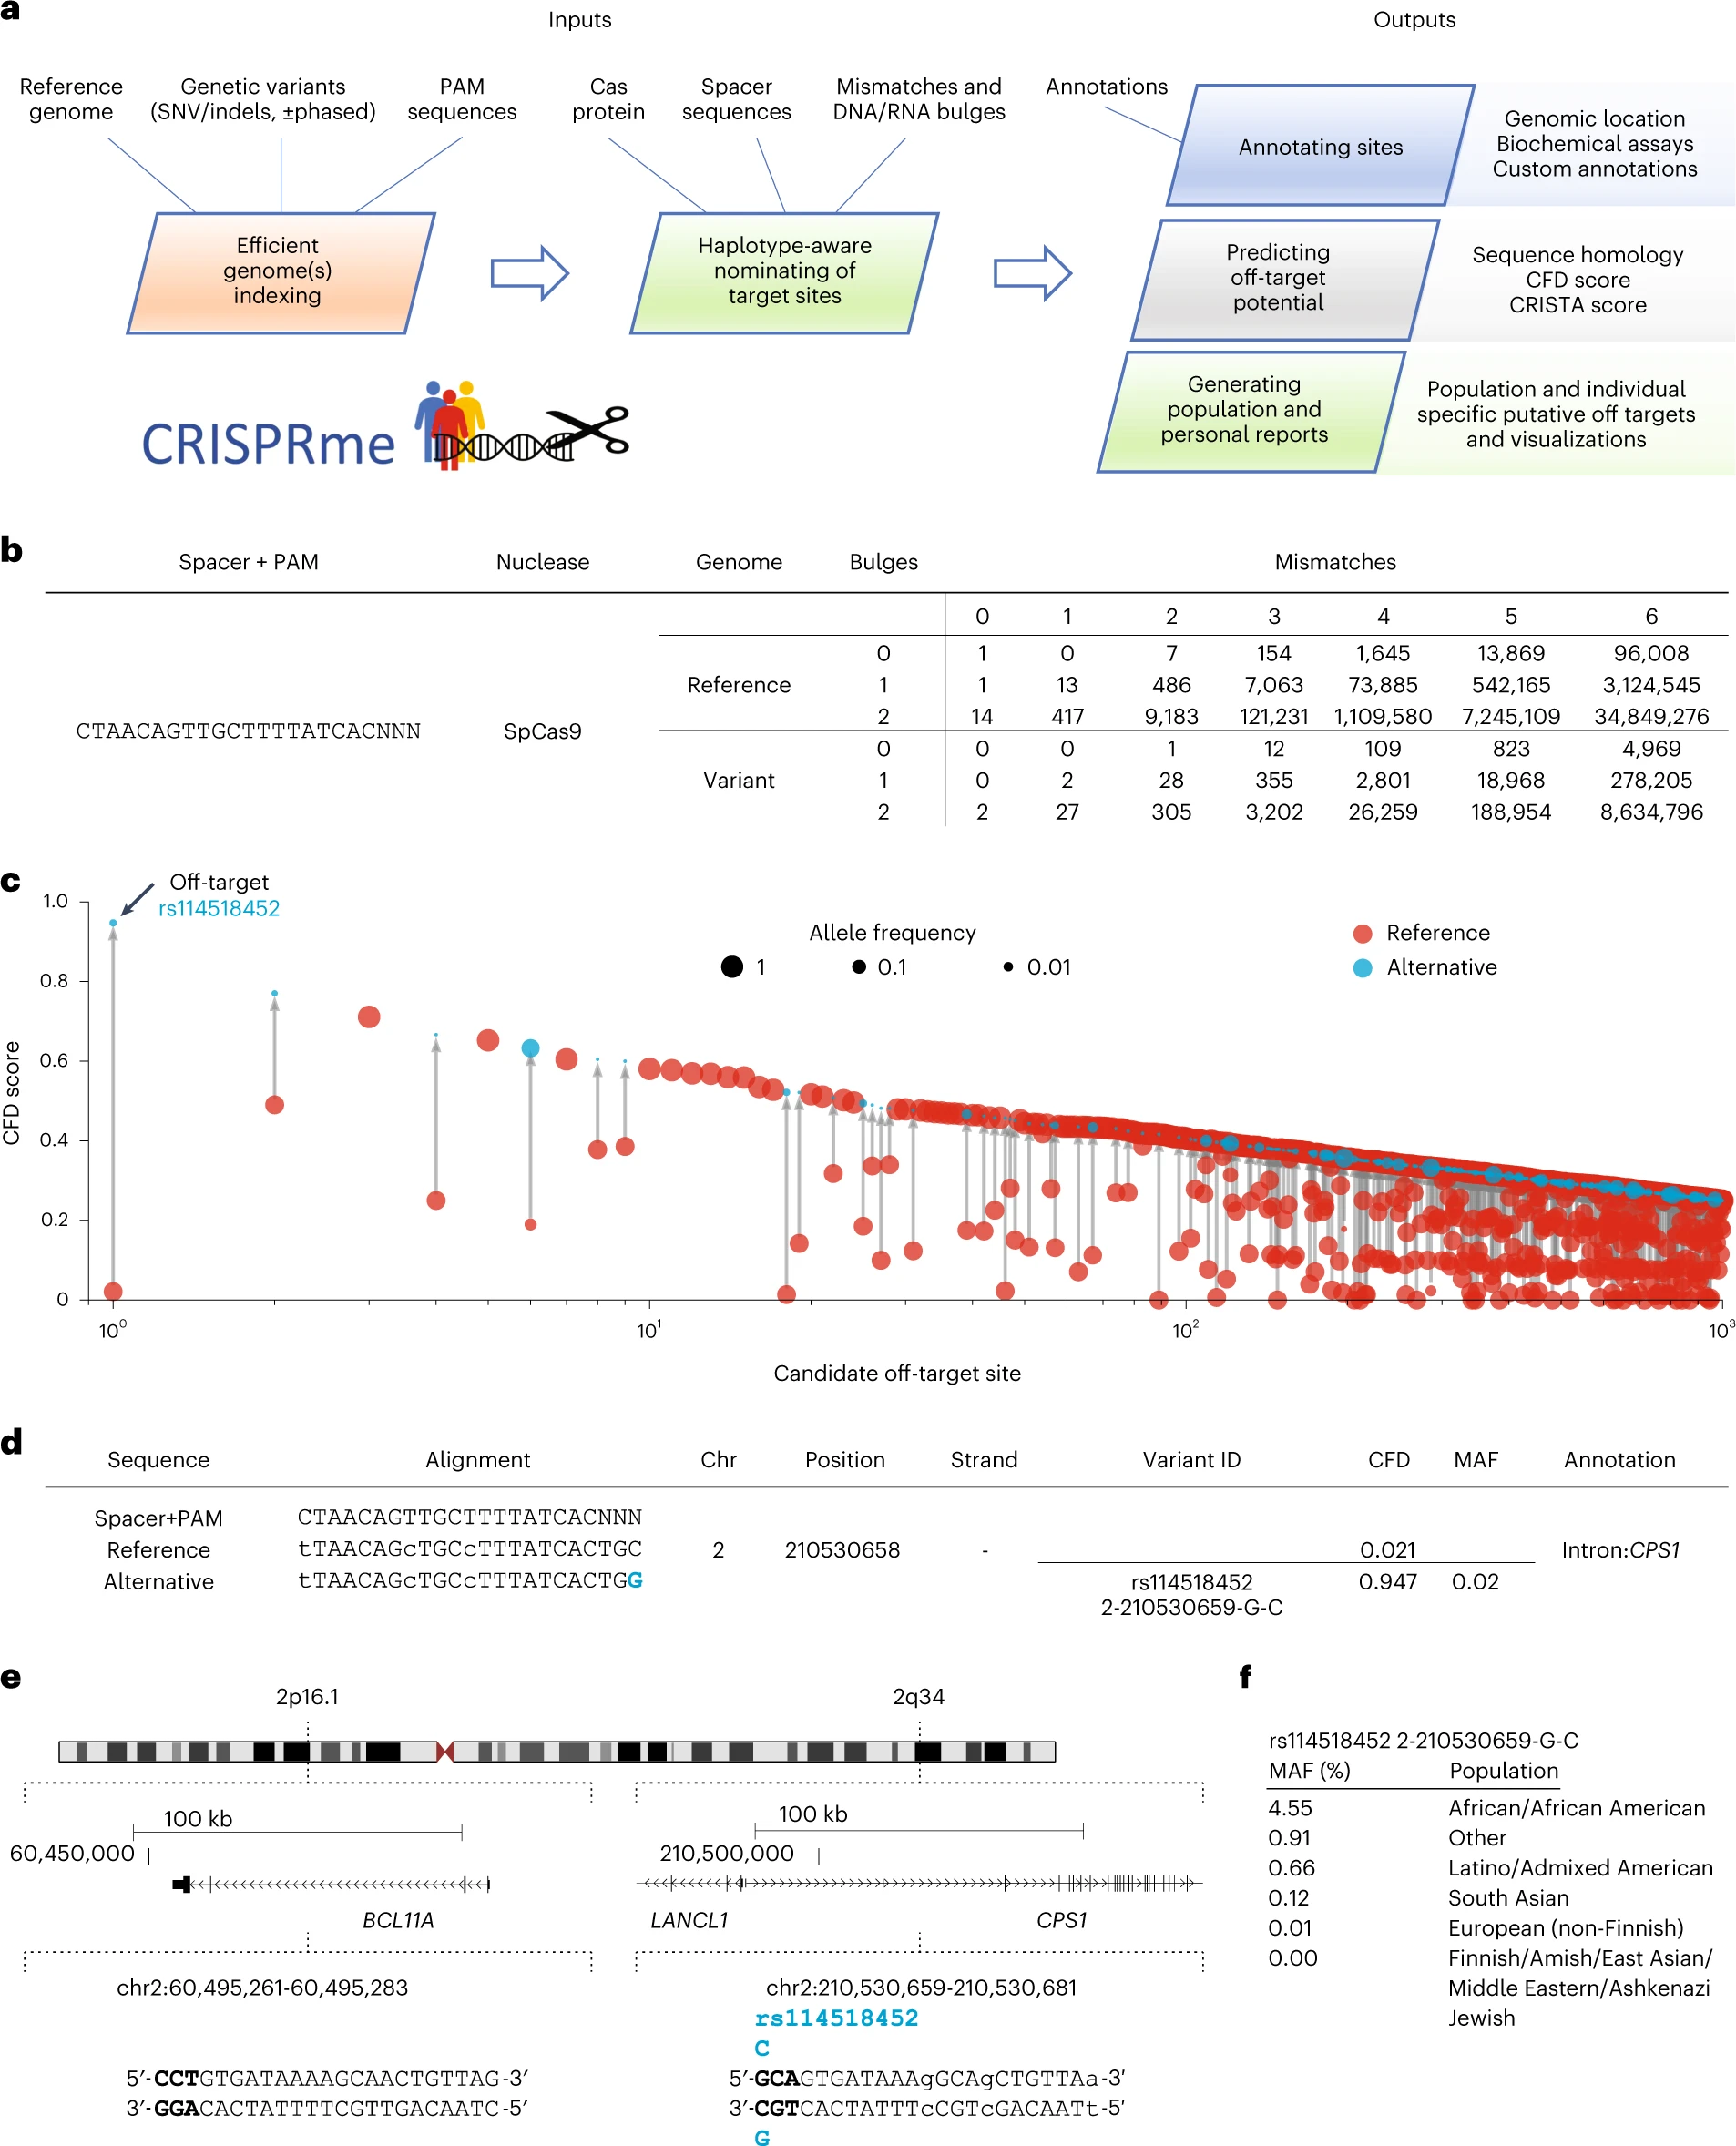
\includegraphics[width=\textwidth]{figures/crisprme1.png}
	\caption[CRISPRme provides web-based analysis of CRISPR-Cas gene editing off-target potential reflecting population genetic diversity]{\textbf{CRISPRme provides web-based analysis of CRISPR-Cas gene editing off-target potential reflecting population genetic diversity. (A)} CRISPRme software takes as input a reference genome, genetic variants, PAM sequence, Cas protein type, spacer sequence, homology threshold and genomic annotations and provides comprehensive, target-focused and individual-focused analyses of off-target potential. It is available as an online webtool and can be deployed locally or used offline as command-line software. \textbf{(B)} Analysis of the BCL11A-1617 spacer targeting the +58 erythroid enhancer with SpCas9, \texttt{NNN} PAM, 1000G variants, up to 6 mismatches and up to 2 bulges. \textbf{(C)} Top 1000 predicted off-target sites ranked by CFD score, indicating the CFD score of the reference and alternative allele if applicable, with allele frequency indicated by circle size. \textbf{(D)} The off-target site with the highest CFD score is created by the minor allele of rs114518452. Coordinates are for hg38 and 0-start for the potential off-target and 1-start for the variant-ID. MAF is based on 1000G. \textbf{(E)} The top predicted off-target site from CRISPRme is an allele-specific off-target with 3 mismatches to the BCL11A-1617 spacer sequence, where the rs114518452-C minor allele produces a de novo NGG PAM sequence. PAM sequence shown in bold and mismatches to BCL11A-1617 shown as lowercase. Coordinates are for hg38 and 1-start. \textbf{(F)} rs114518452 allele frequencies based on gnomAD v3.1. Coordinates are for hg38 and 1-start. Spacer shown as DNA sequence for ease of visual alignment.}
	\label{fig:crisprme1}
\end{figure} 
\crisprme is a web-based tool to predict off-target potential of CRISPR gene editing that accounts for genetic variation. It is available online at \url{http://crisprme.di.univr.it}. \crisprme can also be deployed to local, protected and isolated environments as a web app or command line utility, neither of which transfer or store data online, therefore respecting genomic privacy and regulations. \crisprme takes as input a Cas protein, gRNA spacer sequence and PAM, genome build, sets of variants (VCF files for populations or individuals), user-defined thresholds of mismatches and bulges and optional user-defined genomic annotations to produce comprehensive and personalized reports (\textbf{Fig.\ref{fig:crisprme1}(A)}). We have designed \crisprme to be flexible with support for new gene editors with variable and extremely relaxed PAM requirements \citep{walton2020unconstrained}. Thanks to a PAM encoding based on Aho-Corasick automata and an index based on a ternary search tree, CRISPRme can perform genome-wide exhaustive searches efficiently even with an NNN PAM, extensive mismatches (tested with up to seven) and RNA:DNA bulges (tested with up to two). Notably, a comprehensive search performed with up to six mismatches, two DNA/RNA bulges and a fully nonrestrictive PAM (NNN) on a small computational cluster node using 20 CPUs and 128 GB RAM (Intel Xeon CPU E5-2609 v4 clocked at 2.2 GHz) takes $\sim$34 h of real time and $\sim$152 h of CPU time (including both user and system times). All the 1000 G variants, including both single-nucleotide variants and indels, can be included in the search together with all the available metadata for each individual (sex, superpopulation and age), and the search operation takes into account observed haplotypes. Importantly, off-target sites that represent alternative alignments to a given genomic region are merged to avoid inflating the number of reported sites. Although several tools exist to enumerate off-targets, to our knowledge, only two command line tools \citep{lessard2017human, fennell2021calitas} incorporate genetic variants in the search. However, they have several limitations in terms of scalability to large searches, number of mismatches, bulges, haplotypes and variant file formats supported and do not provide an easy-to-use GUI. \crisprme generates several reports. (i) it summarizes for each gRNA all the potential off-targets found in the reference or variant genomes based on their mismatches and bulges (\textbf{Fig.\ref{fig:crisprme1}(B)}) and generates a file with detailed information on each of these candidate off-targets. 
(ii) it compares gRNAs to customizable annotations. By default, it classifies possible off-target sites based on GENCODE \citep{frankish2019gencode} (genomic features) and ENCODE \citep{encode2012integrated} (candidate cis-regulatory elements (cCREs)) annotations. It can also incorporate user-defined annotations in BED format, such as empiric off-target scores or cell-type-specific chromatin features (\textbf{Fig.\ref{fig:crisprme2}}).  
\begin{figure}
	\centering
	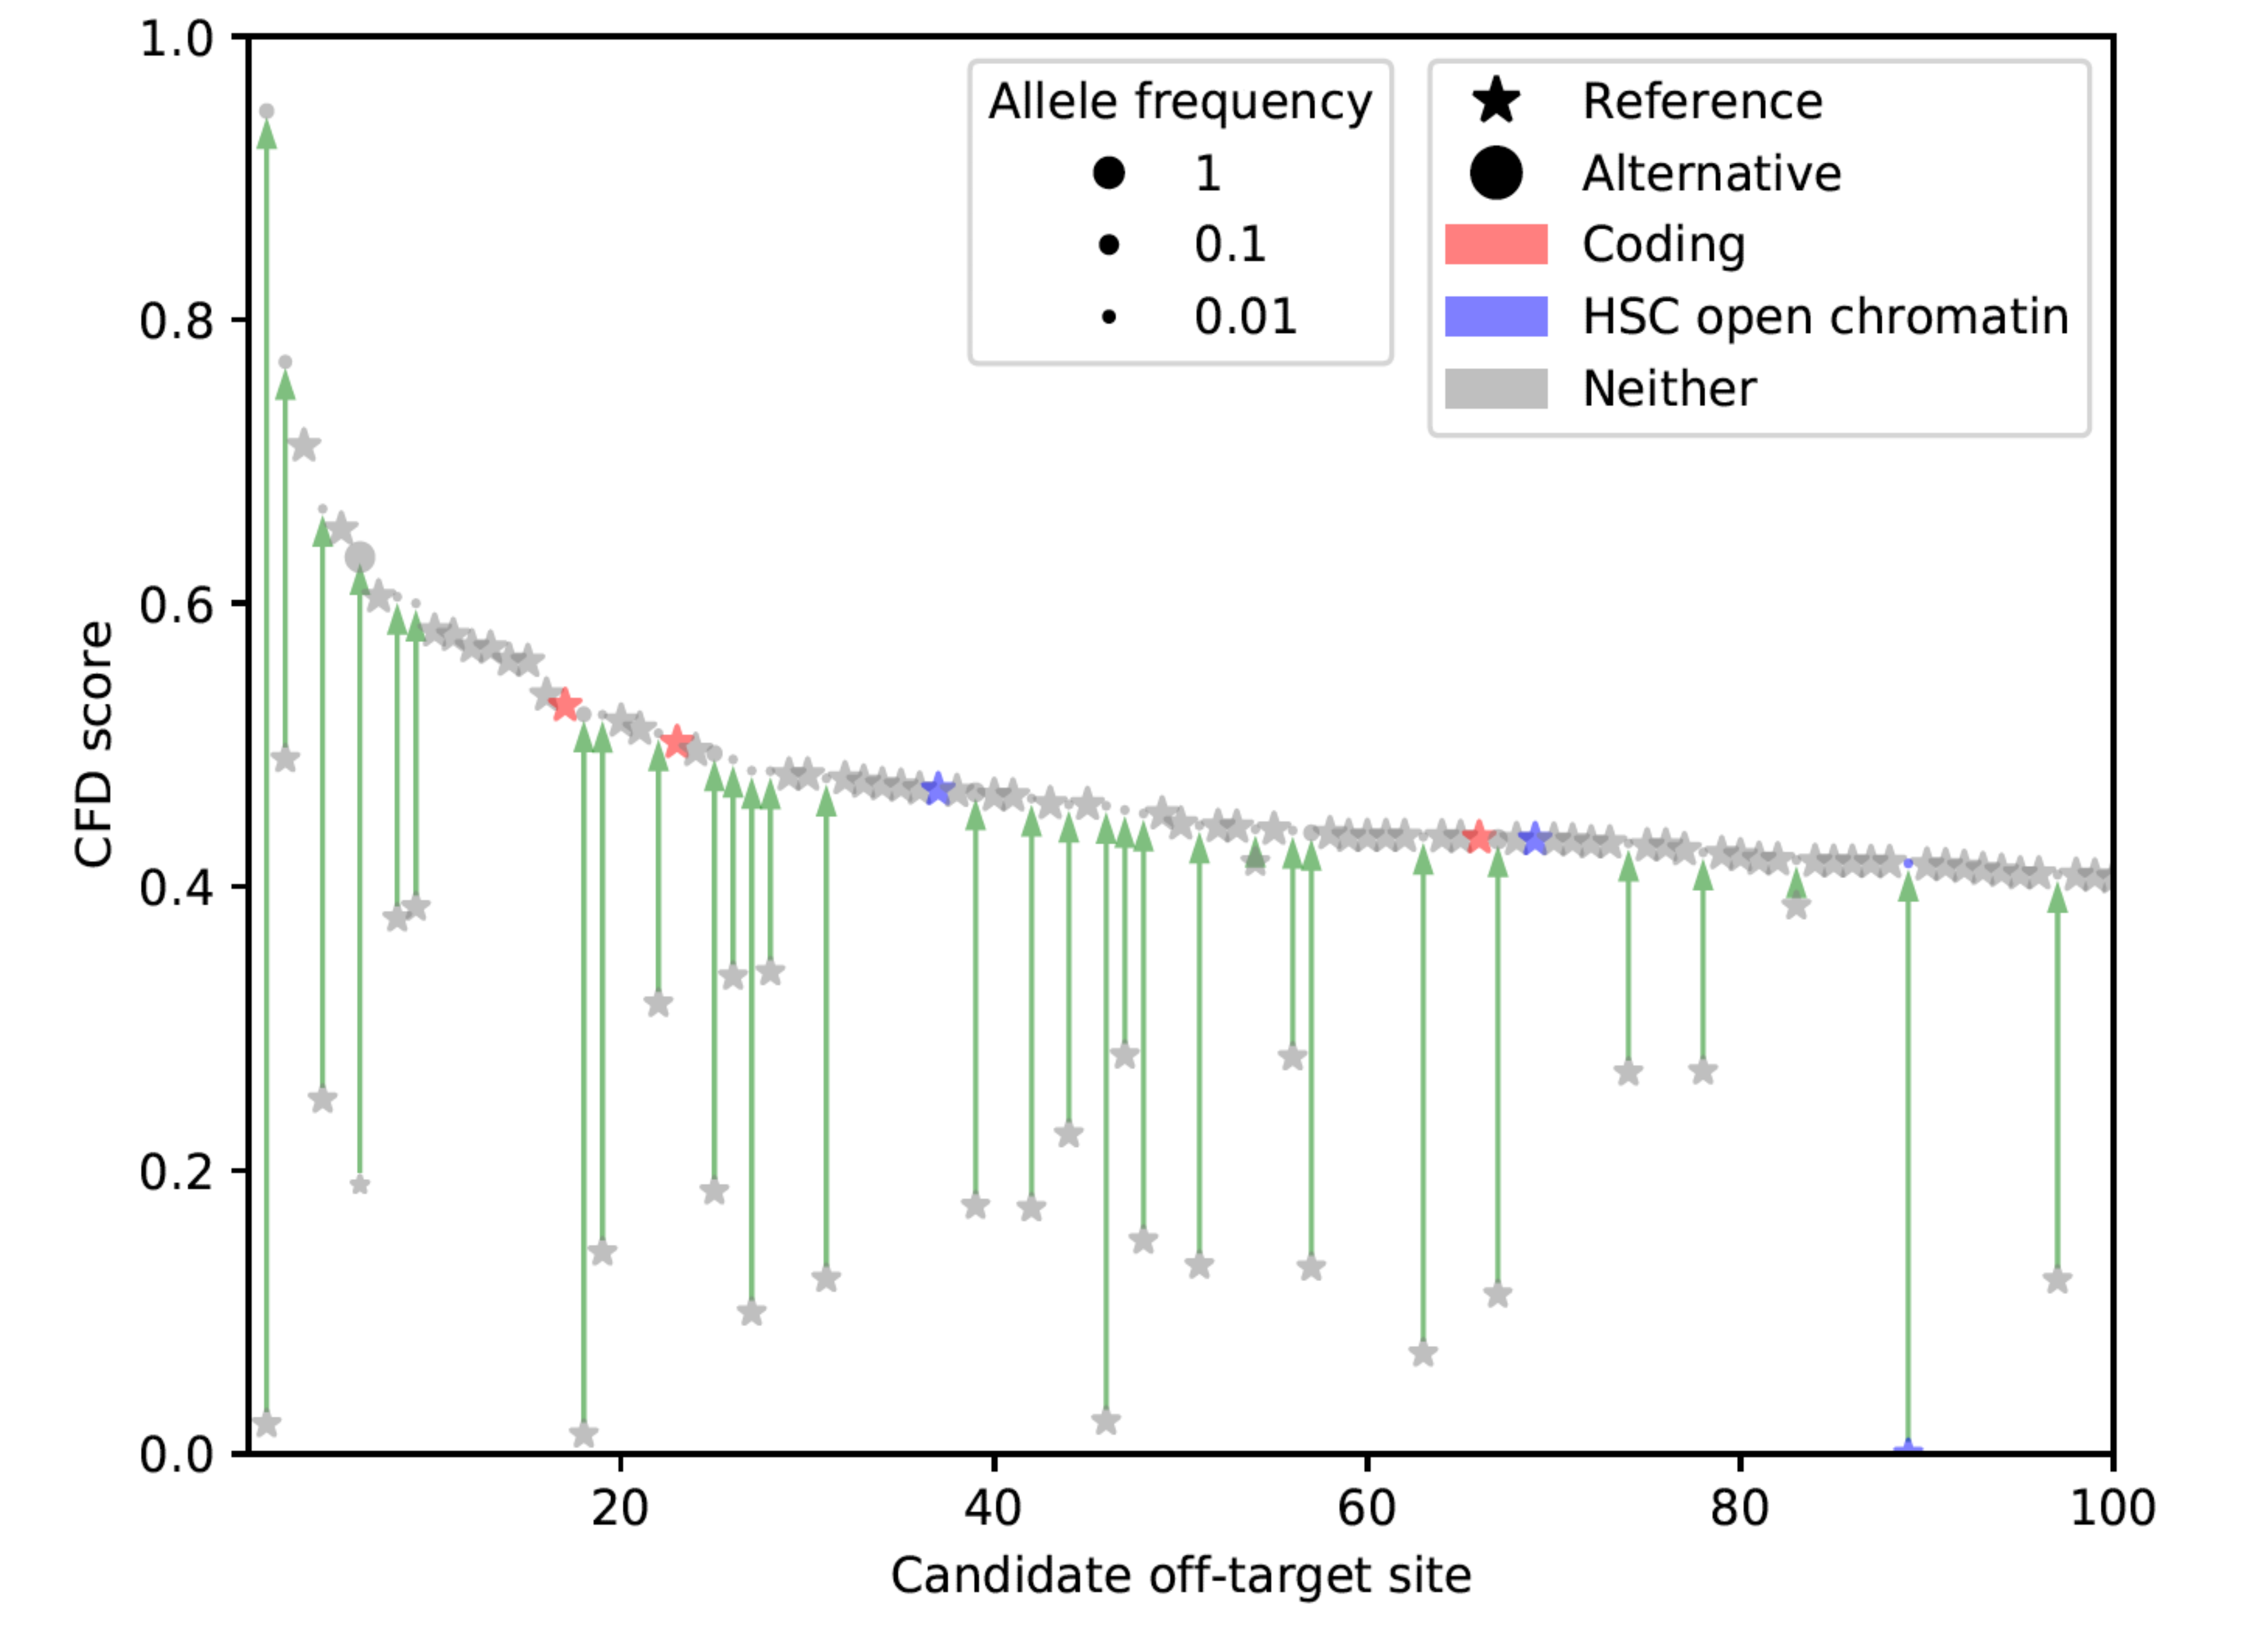
\includegraphics[width=\textwidth]{figures/crisprme2.png}
	\caption[Top 100 predicted off-target sites for BCL11A-1617 spacer by CFD score]{\textbf{Top 100 predicted off-target sites for BCL11A-1617 spacer by CFD score.} \crisprme search as in \textbf{Fig.\ref{fig:crisprme1}}. Candidate off-target sites within coding regions based on GENCODE annotations and ATAC-seq peaks in HSCs based on user-provided annotations (data from \citep{corces2016lineage}) are highlighted.}
	\label{fig:crisprme2}
\end{figure}
(iii) using 1000 G and/or HGDP variants, \crisprme reports the cumulative distribution of homologous sites based on the reference genome or superpopulation. These global reports could be used to compare a set of gRNAs based on how genetic variation impacts their predicted on- and off-target cleavage potential using cutting frequency determination (CFD) or CRISPR Target Assessment (CRISTA) scores \citep{abadi2017machine} (\textbf{Fig.\ref{fig:crisprme3}}). CRISPRme includes multiple scoring metrics and can be easily extended with new ones, including scores tailored for different editors. Finally, CRISPRme can generate personal genome focused reports called personal risk cards. These reports highlight private off-target sites due to unique genetic variants.
\begin{figure}
	\centering
	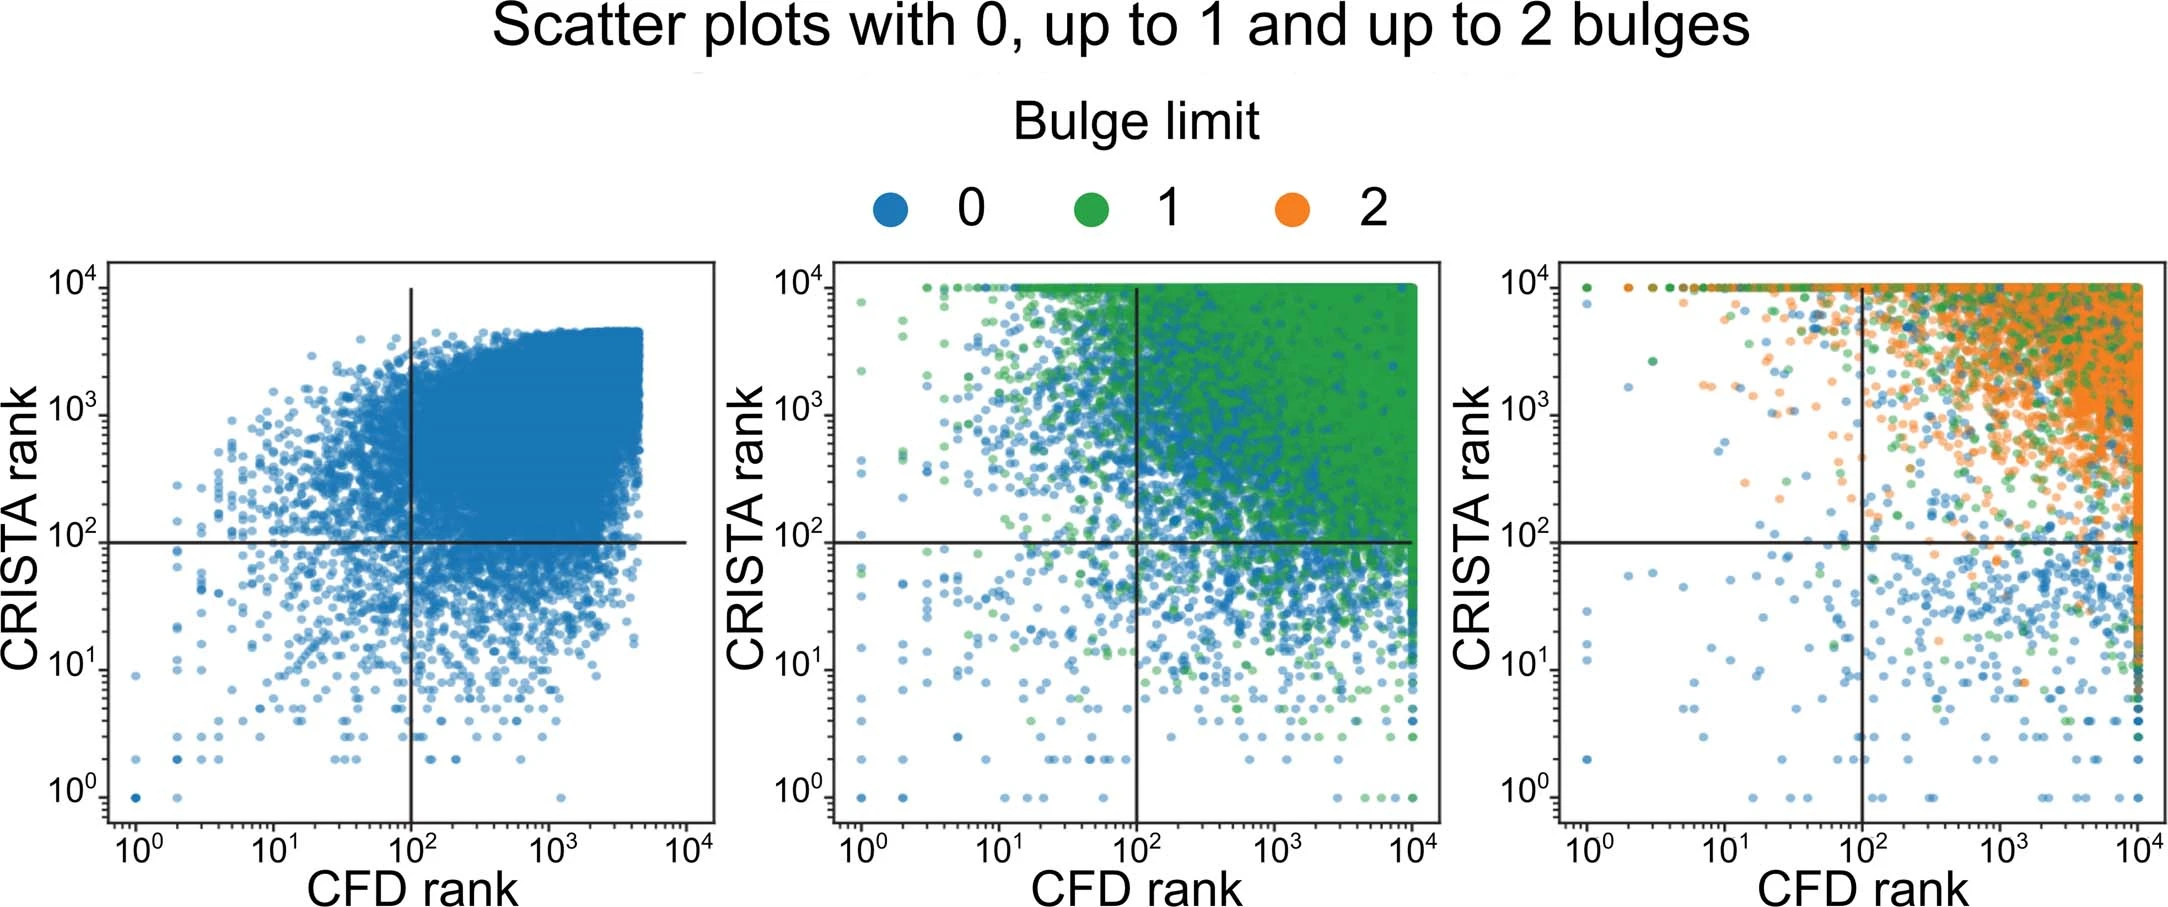
\includegraphics[width=\textwidth]{figures/crisprme3.png}
	\caption[Plots with rank ordered correlation between CFD and CRISTA reported targets]{\textbf{Plots with rank ordered correlation between CFD and CRISTA reported targets.} Scatter plots show from left to right, the correlation of ranked targets, extracted by selecting top 10,000 targets sorted by CFD and CRISTA score, respectively. The left plot shows the rank correlation of targets with 0 bulges (Pearson's correlation: 0.57, $p < 1e^{-10}$, Spearman's correlation: 0.55, $p < 1e^{-10}$), the center plot shows the rank correlation of targets with 1 bulge (Pearson's correlation: -0.16, $p < 1e^{-10}$, Spearman's correlation: -0.33, $p < 1e^{-10}$) and the right plot shows the rank correlation of targets with 2 bulges (Pearson's correlation: -0.55, $p < 1e^{-10}$, Spearman's correlation: -0.80, $p < 1e^{-10}$). The correlation values and $p$-values (two-sided) were calculated using standard functions from the Python scipy library. The colors represent the lowest count of bulges for each target, because the two scoring methods may prioritize different alignments and thus different number of mismatches and bulges pf the same target.}
	\label{fig:crisprme3}
\end{figure}
% -- A common allele-specific off-target for a gRNA in the clinic
\subsection{A common allele-specific off-target for a gRNA in the clinic}
\begin{figure}
	\centering
	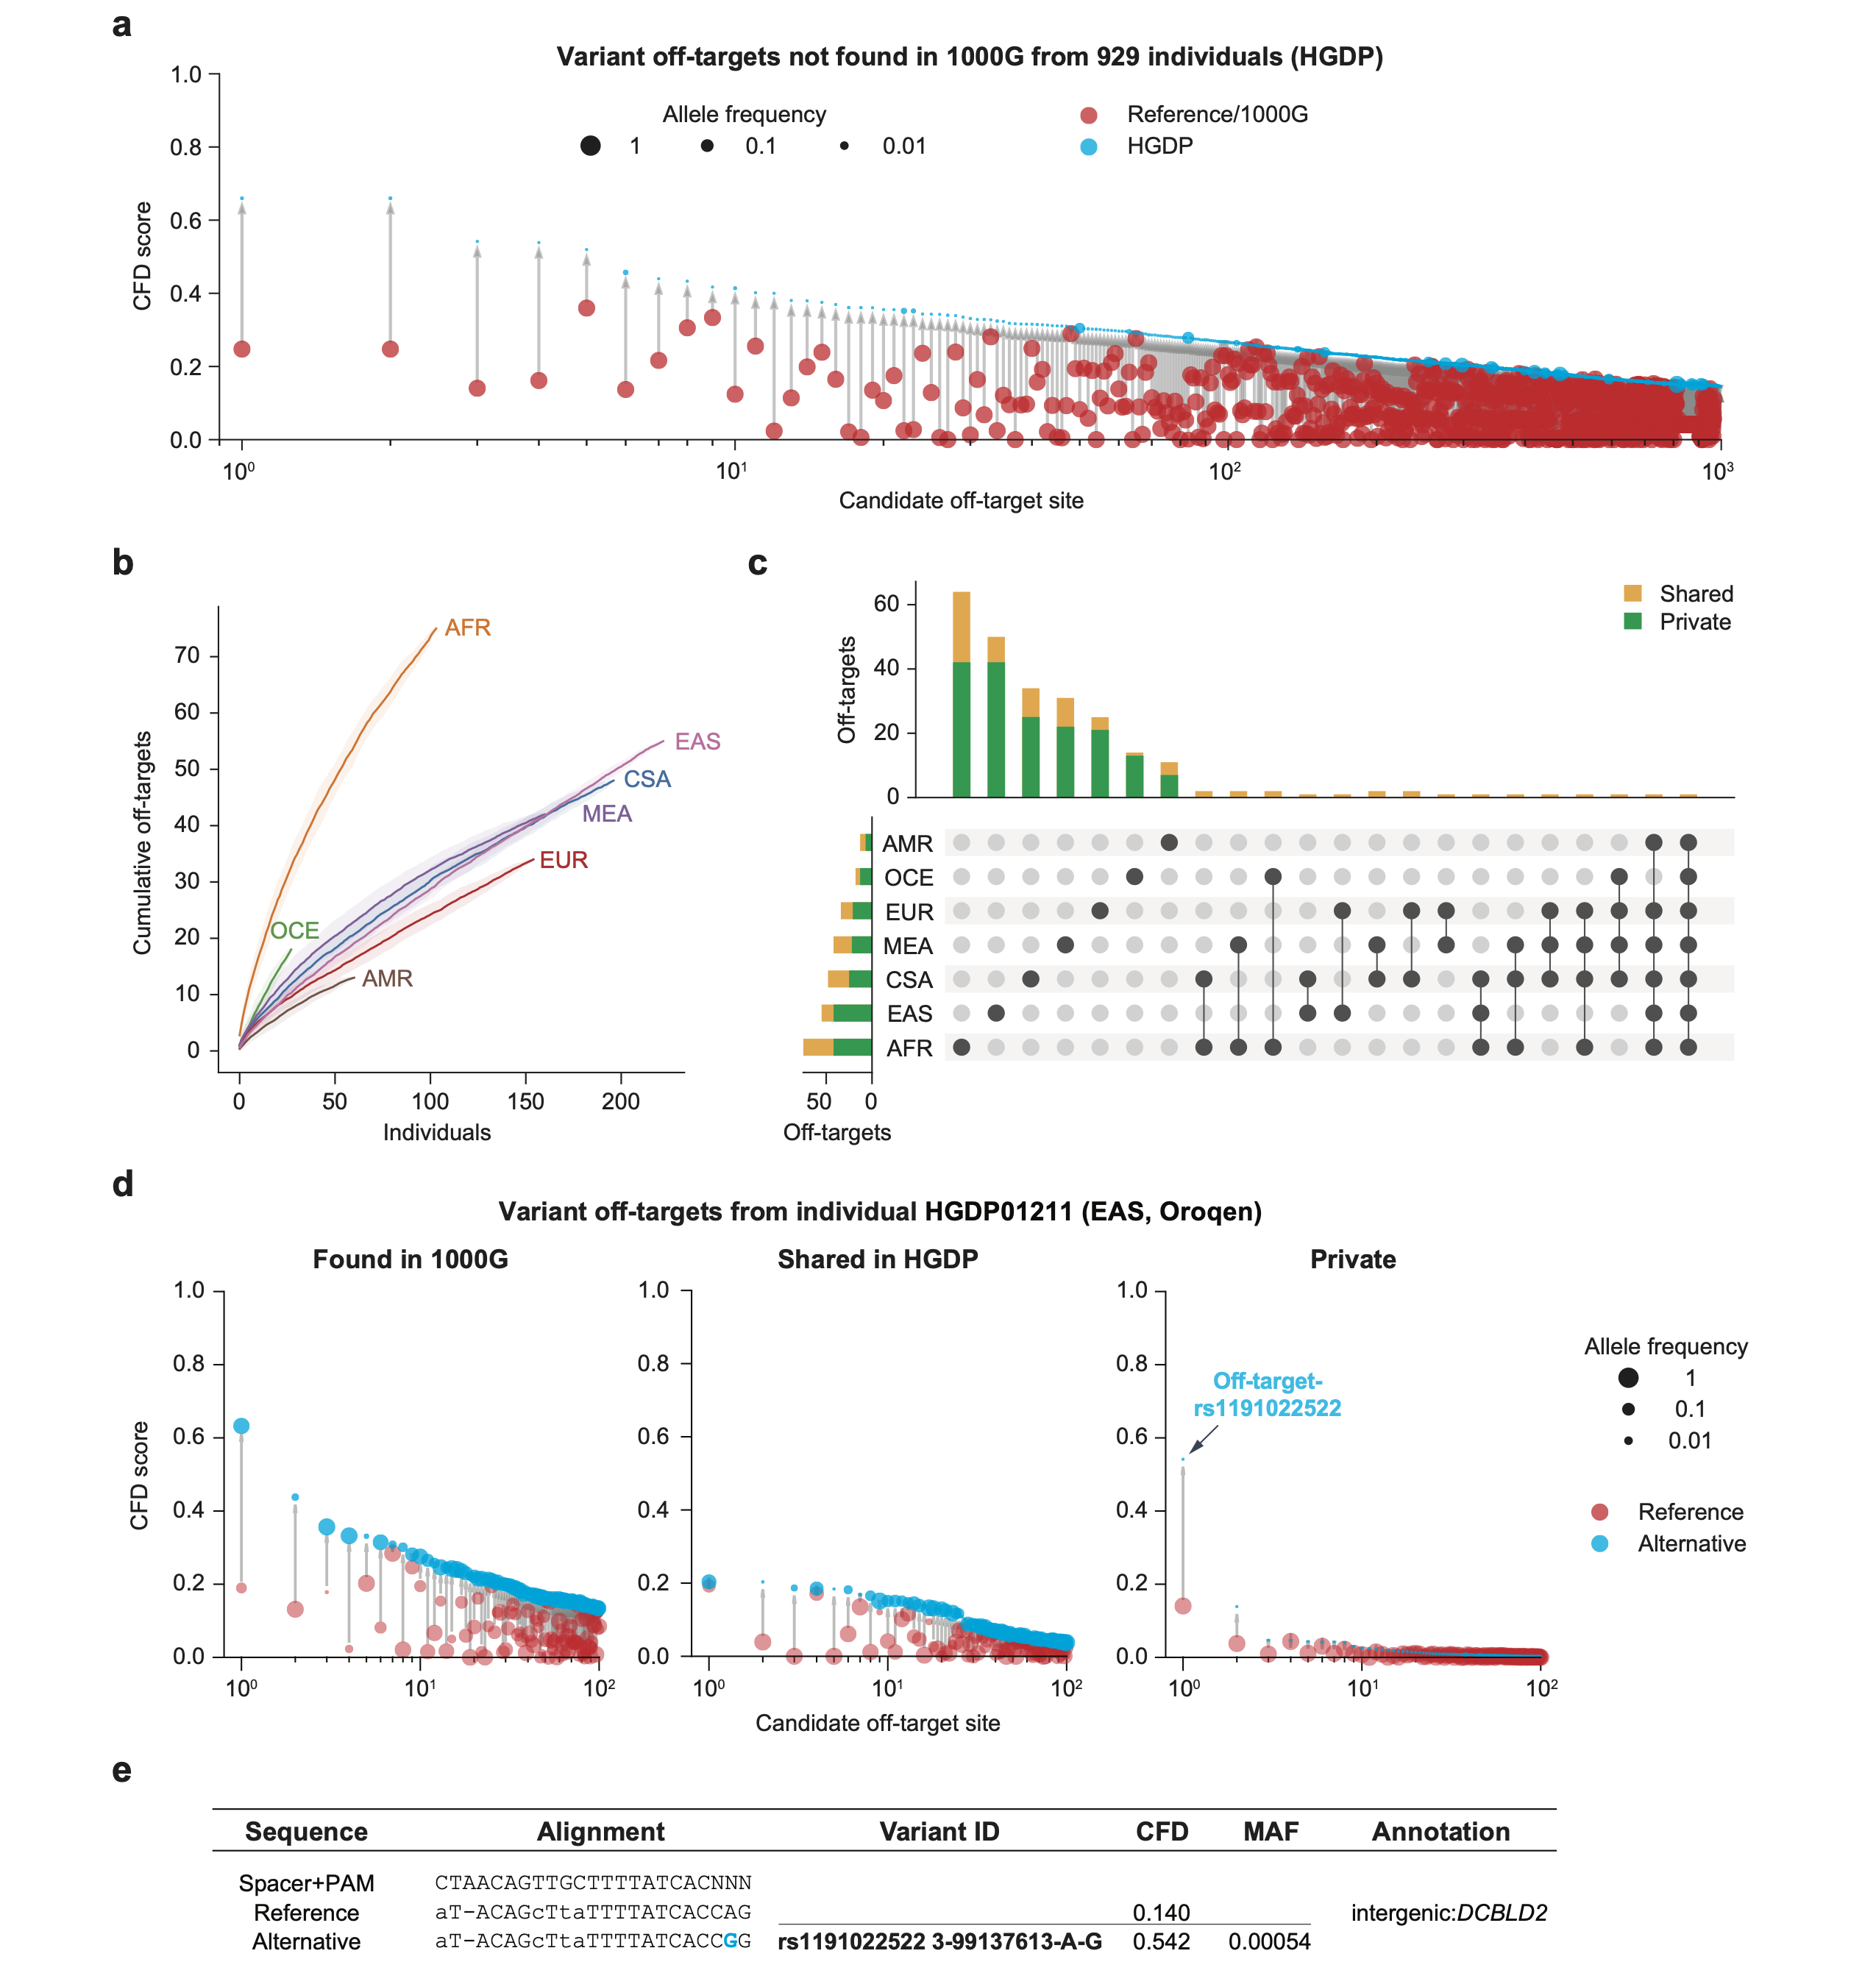
\includegraphics[width=\textwidth]{figures/crisprme4.png}
	\caption[\crisprme provides analysis of off-target potential of CRISPR-Cas gene editing reflecting population and private genetic diversity]{\textbf{\crisprme provides analysis of off-target potential of CRISPR-Cas gene editing reflecting population and private genetic diversity. (A)} \crisprme analysis was conducted with variants from HGDP comprising whole-genome sequencing of 929 individuals from 54 diverse human populations. HGDP variant off-targets with greater CFD scores than the reference genome or 1000 G were plotted and sorted by CFD score, with HGDP variant off-targets shown in blue and reference or 1000 G variant off-targets shown in red. \textbf{(B)} Cumulative distribution plot of HGDP variant off-targets with CFD $\geq 0.2$ and increase in CFD of $\geq 0.1$ per superpopulation (AFR: Africa, AMR: Americas, CSA: Central \& South Asia, EAS: East Asia, EUR: Europe, MEA: Middle East, OCE: Oceania). Individual samples from each of the seven superpopulations were shuffled 100 times to calculate the mean and 95\% confidence interval (shading around lines).  \textbf{(C)} Intersection analysis of HGDP variant off-targets with CFD $\geq 0.2$ and increase in CFD of $\geq 0.1$. Shared variants (black) were found in two or more HGDP samples whereas private variants (gray) were limited to a single sample. \textbf{(D)} \crisprme analysis of a single individual (HGDP01211) showing the top 100 variant off-targets from each of the following three categories: shared with 1000G variant off-targets (left panel), higher CFD score compared to reference genome and 1000 G but shared with other HGDP individuals (center panel) and higher CFD score compared to reference genome and 1000 G with variant not found in other HGDP individuals (right panel). For the center and right panels, reference refers to CFD score from reference genome or 1000 G variants.  \textbf{(E)} The top predicted private off-target site from HGDP01211 is an allele-specific off-target where the rs1191022522-G minor allele produces a canonical NGG PAM sequence in place of a noncanonical NAG PAM sequence. Spacer shown as DNA sequence for ease of visual alignment.}
	\label{fig:crisprme4}
\end{figure}
We tested \crisprme with a gRNA (\#1617) targeting a GATA1 binding motif at the +58 erythroid enhancer of BCL11A \citep{canver2015bcl11a, wu2019highly}. A recent clinical report described two patients, one with SCD and one with $\beta$-thalassemia, each treated with autologous gene modified HSPCs edited with Cas9 and this gRNA, who showed sustained increases in fetal hemoglobin, transfusion independence and absence of vaso-occlusive episodes (in the patient with SCD) following therapy. This study, as well as prior preclinical studies with the same gRNA (\#1617), did not reveal evidence of off-target editing in treated cells when considering off-target sites nominated by bioinformatic analysis of the human reference genome and empiric analysis of in vitro genomic cleavage potential \citep{frangoul2021crispr, wu2019highly, demirci2019durable}.  \crisprme analysis found that the predicted off-target site with both the greatest CFD score and the greatest increase in CFD score from the reference to alternative allele was at an intronic sequence of CPS1 (\textbf{Fig.\ref{fig:crisprme1}(C)} and \textbf{(D)}),  a genomic target subject to common genetic variation (modified by a SNP with MAF $\geq$ 1\%). CFD scores range from 0 to 1, where the on-target site has a score of 1. The alternative allele rs114518452-C generates a TGG PAM sequence (that is, the optimal PAM for SpCas9) for a potential off-target site with three mismatches and a CFD score (CFD$_{alt}$ 0.95) approaching that of the on-target site (\textbf{Fig.\ref{fig:crisprme1}(E)}). In contrast, the reference allele rs114518452-G disrupts the PAM to TGC, which markedly reduces predicted cleavage potential (CFD$_{ref}$ 0.02). rs114518452-C has an overall MAF of 1.33\% in gnomAD v3.1, with an MAF of 4.55\% in African/African American, 0.91\% in Other, 0.66\% in Latino/Admixed American, 0.12\% in South Asian, 0.01\% in European (non-Finnish) and 0.00\% in all other populations represented in gnomAD (\textbf{Fig.\ref{fig:crisprme1}(F)}). To consider the off-target potential that could be introduced by personal genetic variation that would not be predicted by 1000 G variants, we analyzed HGDP variants identified from whole-genome sequences of 929 individuals from 54 diverse human populations. We observed 249 candidate off-targets for gRNA \#1617 with CFD $\geq 0.2$ for which the CFD score in HGDP exceeded that found for either the reference genome or 1000 G variants by at least 0.1 (\textbf{Fig.\ref{fig:crisprme4}(A)} and \textbf{Fig.\ref{fig:crisprme5}}). hese additional variant off-targets not found from 1000 G were observed in each superpopulation, with the greatest frequency in the African superpopulation (\textbf{Fig.\ref{fig:crisprme4}(B)}); 229 (92.0\%) of these variant off-targets were unique to a superpopulation, and 172 (69.1\%) of these were private to just one individual (\textbf{Fig.\ref{fig:crisprme4}(C)}). Furthermore, single-individual-focused searches (for example, an analysis of HGDP01211, an individual of the Oroqen population within the East Asian superpopulation) showed that most variant off-targets (with higher CFD score than reference) were due to variants also found in 1000 G (n = 32369, 90.4\%), a subset were due to variants shared with other individuals from HGDP but absent from 1000 G (n = 3177, 8.9\%) and a small fraction were private to the individual (n = 234, 0.7\%) (\textbf{Fig.\ref{fig:crisprme4}(D)}).  Among these private off-targets was one generated by a variant (rs1191022522, 3-99137613-A-G, gnomAD v3.1 MAF 0.0053\%) where the alternative allele produces a canonical NGG PAM that increases the CFD score from 0.14 to 0.54 (\textbf{Fig.\ref{fig:crisprme4}(D)} and \textbf{(E)}).
\begin{figure}
	\centering
	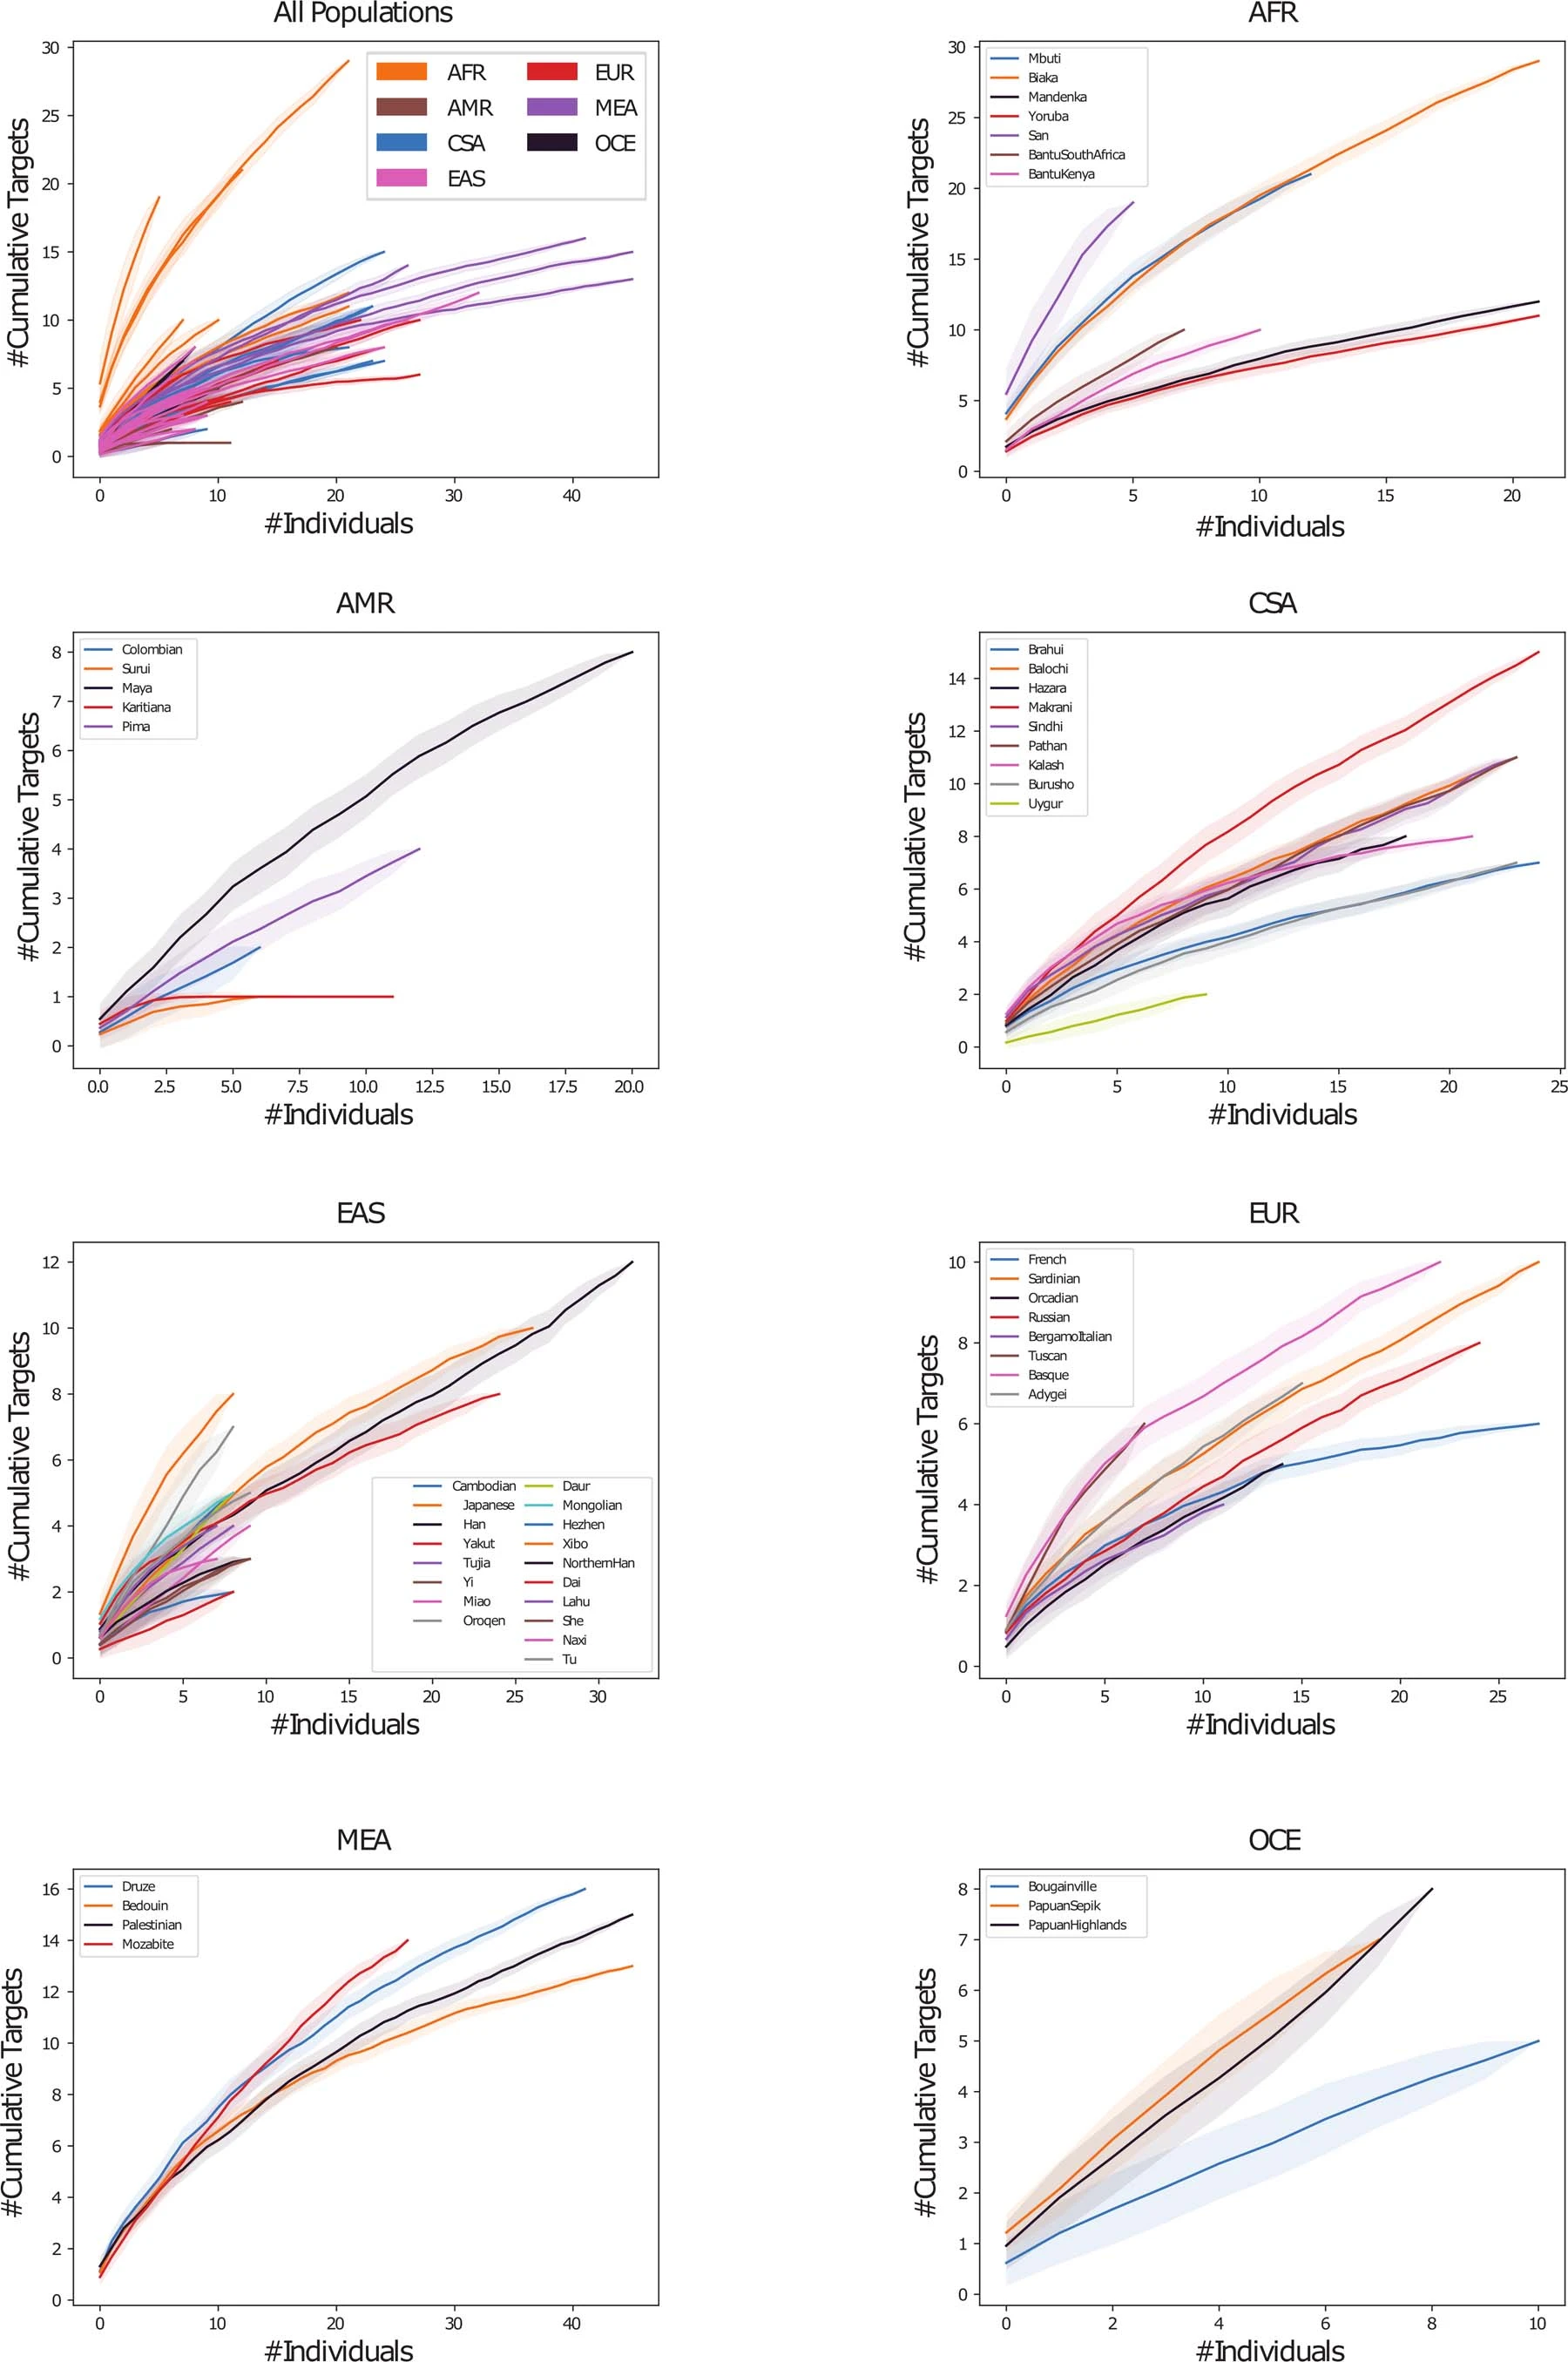
\includegraphics[width=\textwidth]{figures/crisprme5.png}
	\caption[HGDP superpopulation distribution plots]{\textbf{HGDP superpopulation distribution plots.} HGDP variant off-targets with CFD $\geq 0.2$ and increase in CFD of $\geq 0.1$.  Individual samples from each of the seven superpopulations were shuffled 100 times to calculate the mean and 95\% confidence interval. First panel shows distribution within all 54 discrete populations, colored by superpopulation. Additional seven panels show distribution of discrete populations within each listed superpopulation.}
	\label{fig:crisprme5}
\end{figure}
o experimentally test the top predicted off-target from CRISPRme, we identified a CD34+ HSPC donor of African ancestry heterozygous for rs114518452-C, the variant predicted to introduce the greatest increase in off-target cleavage potential (\textbf{Fig.\ref{fig:crisprme1}(C)-(F)}).  We performed ribonucleoprotein (RNP) electroporation using a gene editing protocol that preserves engrafting HSC function. Amplicon sequencing analysis showed 92.0 $\pm$ 0.5\% indels at the on-target site and 4.8 $\pm$ 0.5\% indels at the off-target site. For reads spanning the variant position, indels were strictly found at the alternative PAM-creation allele without indels observed at the reference allele (\textbf{Fig.\ref{fig:crisprme6}(A)-(C)}),  suggesting 9.6 $\pm$ 1.0\% off-target editing of the alternative allele. In an additional six HSPC donors homozygous for the reference allele rs114518452-G/G, 0.00 $\pm$ 0.00\% indels were observed at the off-target site, suggesting strict restriction of off-target editing to the alternative allele (\textbf{Fig.\ref{fig:crisprme6}(D)}).
\begin{figure}
	\centering
	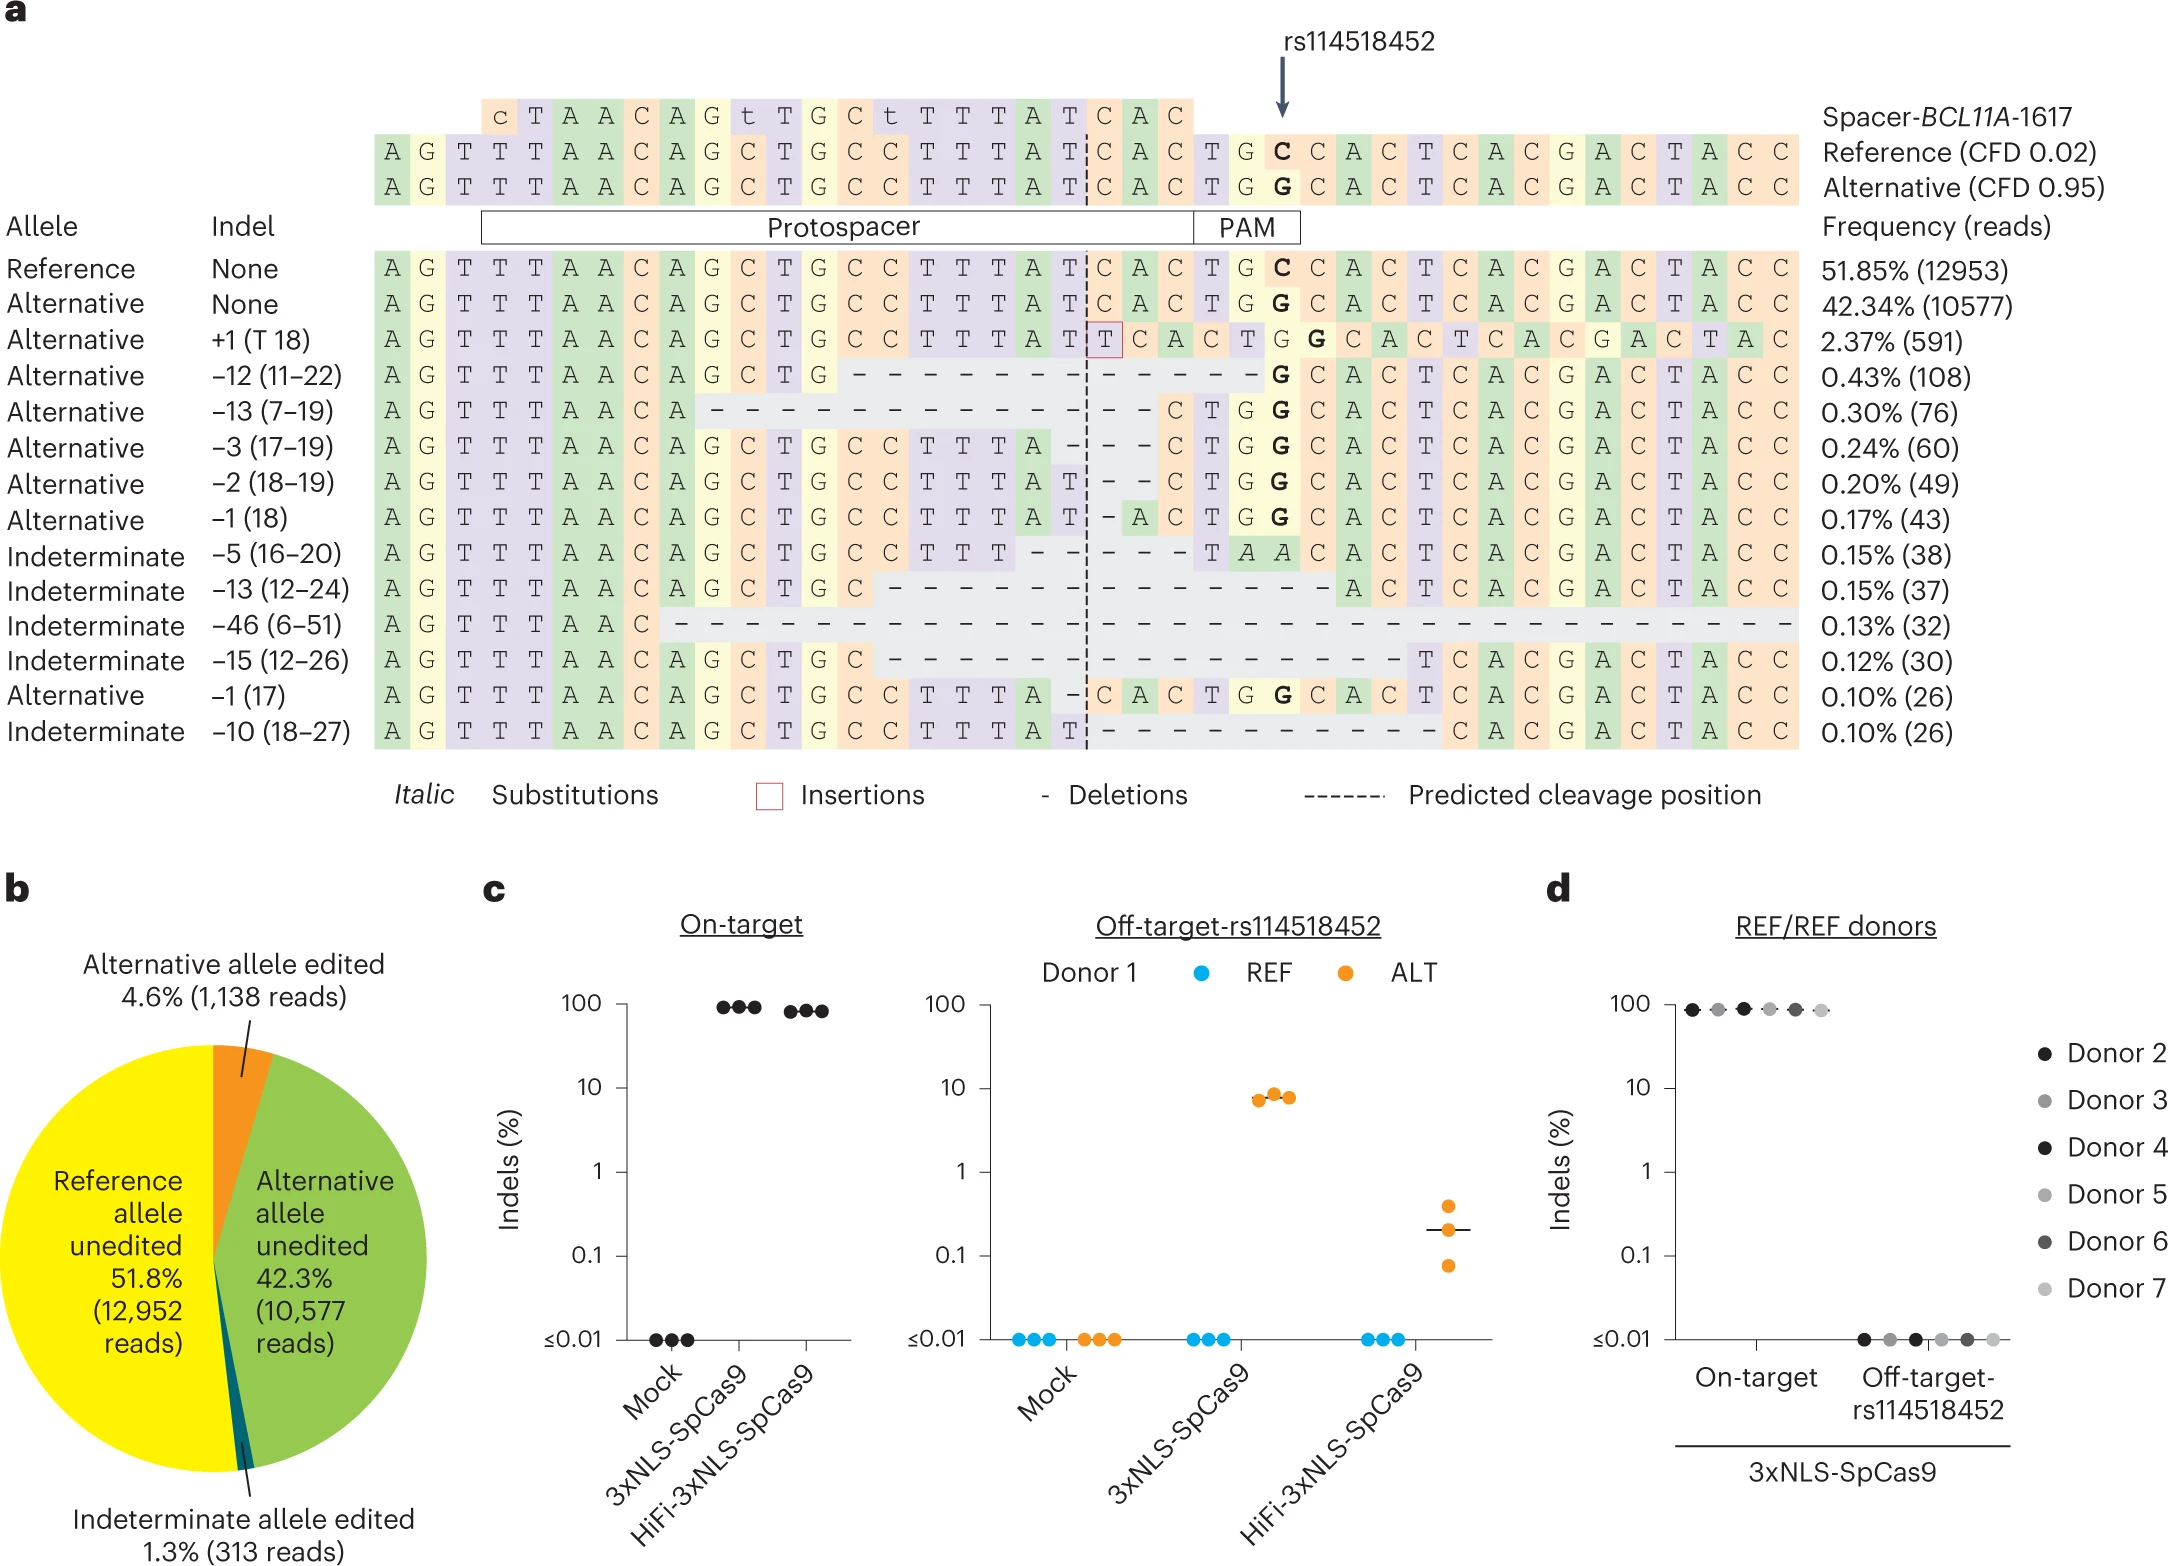
\includegraphics[width=\textwidth]{figures/crisprme6.png}
	\caption[Allele-specific off-target editing by a BCL11A enhancer targeting gRNA in clinical trials associated with a common variant in African-ancestry populations]{\textbf{Allele-specific off-target editing by a BCL11A enhancer targeting gRNA in clinical trials associated with a common variant in African-ancestry populations. (A)} Human CD34+ HSPCs from a donor heterozygous for rs114518452-G/C (donor 1, REF/ALT) were subject to 3xNLS-SpCas9:sg1617 RNP electroporation (NLS: nuclear localization signal) followed by amplicon sequencing of the off-target site around chr2:210,530,659-210,530,681 (off-target-rs114518452 in 1-start hg38 coordinates). CFD scores for the reference and alternative alleles are indicated, and representative aligned reads are shown. Spacer shown as DNA sequence for ease of visual alignment, with mismatches indicated by lowercase and the rs114518452 position shown in bold.  \textbf{(B)} Reads classified based on allele (indeterminate if the rs114518452 position is deleted) and presence or absence of indels (edits). \textbf{(C)} Huma CD34+ HSPCs ffrom a donor heterozygous for rs114518452-G/C (donor 1) were subject to 3xNLS-SpCas9:sg1617 RNP electroporation,  HiFi-3xNLS-SpCas9:sg1617 RNP electroporation, or no electroporation (mock) followed by amplicon sequencing of the on-target and off-target-rs114518452 sites. each dot represents an independentbiological replicate (n = 3), and lines represent medians. Indel frequency was quantified for reads aligning to either the reference (REF) or alternative (ALT) allele. \textbf{(D)} Human CD34+ HSPCs from six donors homozygous for rs114518452-G/G (donors 2–7, REF/REF) were subject to 3xNLS-SpCas9:sg1617 RNP electroporation with one biological replicate per donor followed by amplicon sequencing of the on-target and off-target-rs114518452 sites.}
	\label{fig:crisprme6}
\end{figure}
The on-target BCL11A intronic enhancer site is on chr2p, whereas the off-target-rs114518452 site is on chr2q within an intron of a noncanonical transcript of CPS1. Inversion PCR demonstrated inversion junctions consistent with the presence of $\sim$150 Mb pericentric inversions between BCL11A and the off-target site only in edited HSPCs carrying the alternative allele (\textbf{Fig.\ref{fig:crisprme7}(A)} and \textbf{(B)}). Deep sequencing of the inversion junction showed that inversions were restricted to the alternative allele in the heterozygous cells (\textbf{Fig.\ref{fig:crisprme7}(C)} and \textbf{(D)}). Droplet digital PCR revealed these inversions to be present at 0.16 $\pm$ 0.04\% allele frequency (\textbf{Fig.\ref{fig:crisprme7}(E)}). Various high-fidelity Cas9 variants may improve the specificity of gene editing, although at the possible cost of reduced efficiency \citep{schmid2020highly}. Gene editing following the same electroporation protocol using a HiFi variant 3xNLS-SpCas9 (R691A) \citep{vakulskas2018high} in heterozygous cells revealed 82.3 $\pm$ 1.6\% on-target indels with only 0.1 $\pm$ 0.1\% indels at the rs114518452-C off-target site (that is, a $\sim$48-fold reduction compared to SpCas9) (\textbf{Fig.\ref{fig:crisprme6}(C)}). Inversions were not detected following HiFi-3xNLS-SpCAs9 editing (\textbf{Fig.\ref{fig:crisprme7}(B)} and \textbf{(E)}).
\begin{figure}
	\centering
	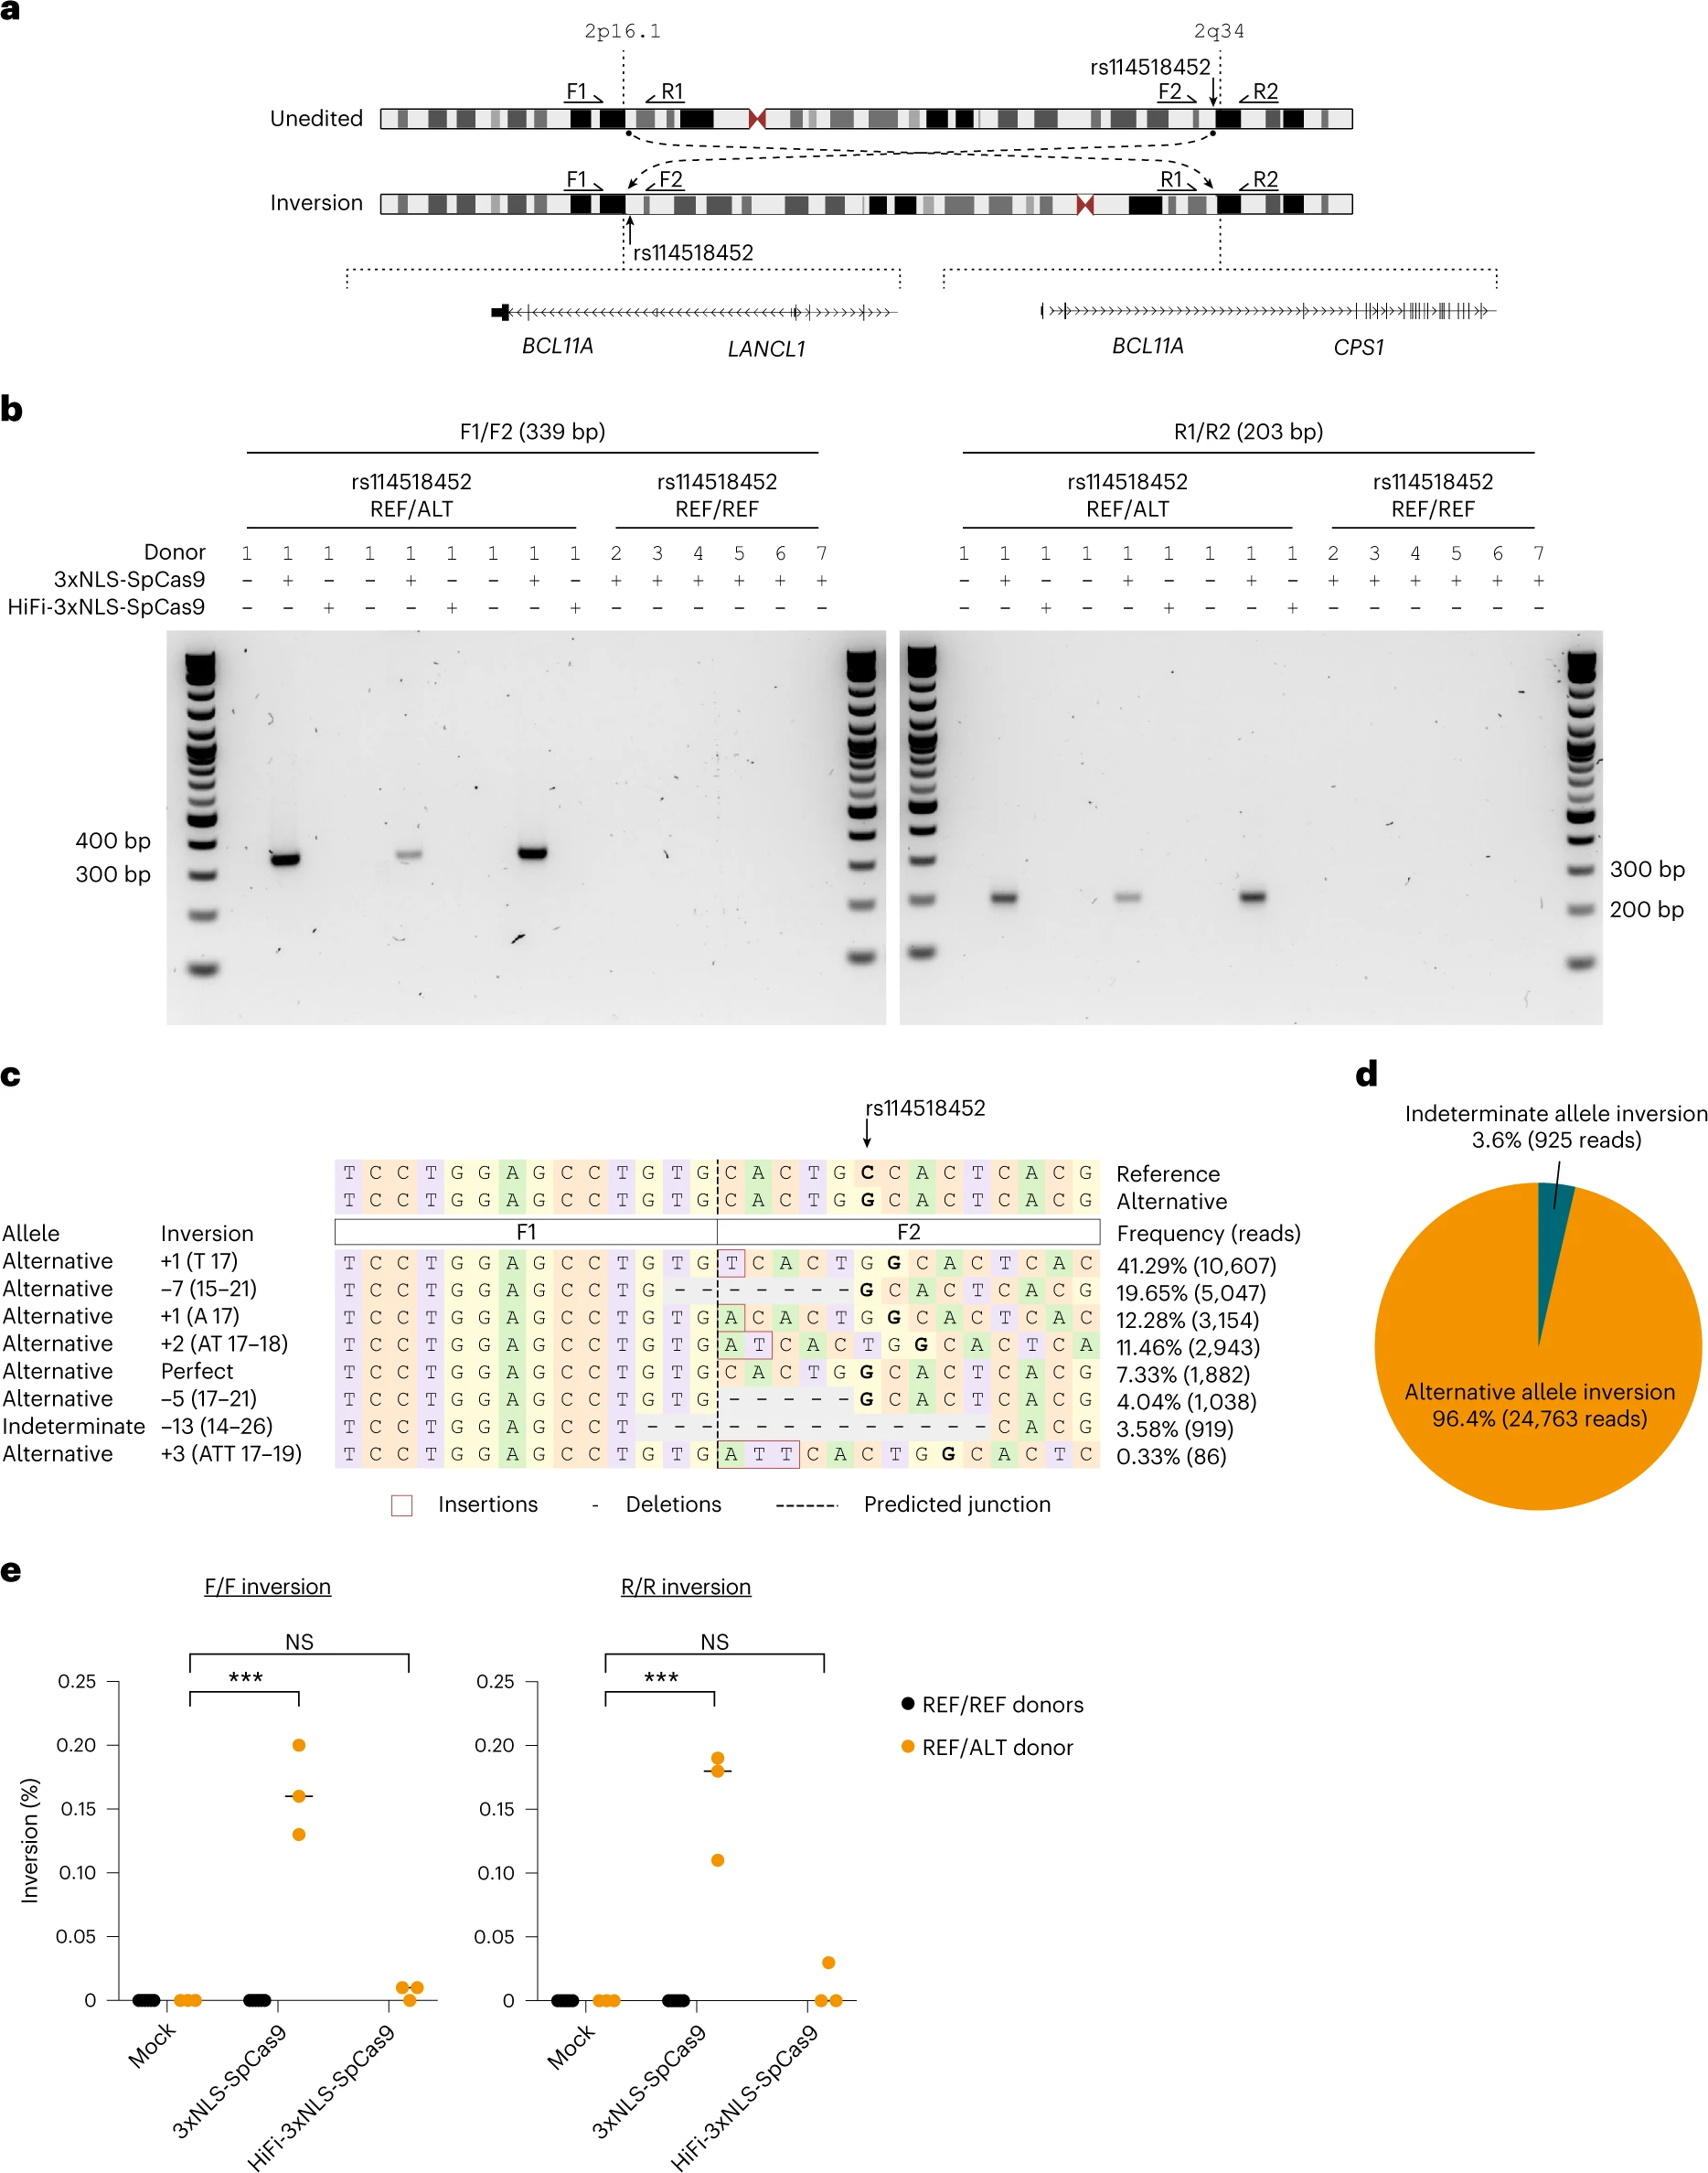
\includegraphics[width=\textwidth]{figures/crisprme7.png}
	\caption[Allele-specific pericentric inversion following BCL11A enhancer editing due to off-target cleavage]{\textbf{Allele-specific pericentric inversion following BCL11A enhancer editing due to off-target cleavage. (A)} Concurrent cleavage of the on-target and off-target-rs114518452 sites could lead to pericentric inversion of chr2 as depicted. PCR primers F1, R1, F2 and R2 were designed to detect potential inversions. \textbf{(B)} Human CD43+ HSPCs from a donor heterozygous for rs114518452-G/C (donor 1) were subject to 3xNLS-SpCas9:sg1617 RNP electroporation, HiFi-3xNLS-SpCas9:sg1617 RNP electroporation or no electroporation with three biological replicates. Human CD43+ HSPCs from six donors homozygous for rs114518452-G/G (donors 2–7, REF/REF) were subject to 3xNLS-SpCas9:sg1617 RNP electroporation with one biological replicate per donor. Gel electrophoresis for inversion PCR was performed with F1/F2 and R1/R2 primer pairs on left and right respectively with expected sizes of precise inversion PCR products indicated. \textbf{(C)} Reads from amplicon sequencing of the F1/F2 product (expected to include the rs114518452 position) from 3xNLS-SpCas9:sg1617 RNP treatment were aligned to reference and alternative inversion templates. The rs114518452 position is shown in bold. \textbf{(D)} Reads classified based on allele (indeterminate if the rs114518452 position deleted). \textbf{(E)} Inversion frequency by droplet digital PCR (ddPCR) from same samples as in panel b with three replicates from the single REF/ALT donor and one replicate each from the six REF/REF donors. F/F indicates forward and R/R reverse inversion junctions as depicted in panel a. NS, not significant.}
	\label{fig:crisprme7}
\end{figure}
% -- Allele specific off-target potential of additional gRNAs
\subsection{Allele specific off-target potential of additional gRNAs}
To examine the pervasiveness of alternative allele off-target potential, we evaluated an additional 13 gRNAs in clinical development or otherwise widely used for SpCas9-based nuclease or base editing \citep{xu2017crispr, xu2019crispr, stadtmauer2020crispr, gillmore2021crispr, dewitt2016selection, xu2019editing, metais2019genome, tsai2015guide, zeng2020therapeutic, musunuru2021vivo} and 6 gRNAs for non-SpCas9-based editing such as for SaCas9 and Cas12a \citep{xu2019editing, chu2021rationally, newby2021base, maeder2019development, de2019edit}. \crisprme analysis including the 1000 G and HGDP genetic variant datasets showed 18\% (95\% confidence interval 13-23\%) of the total nominated off-targets were due to alternative allele-specific off-targets. Most alternative allele-specific off-targets were associated with rare variants (MAF $<$ 1\%),  although candidate off-targets associated with common variants were identified for each gRNA (\textbf{Fig.\ref{fig:crisprme8}(A)}). None of these alternative allele-specific off-target sites were described in the original manuscripts reporting the editing strategies and off-target analyses. CRISPRme produces visualizations to specifically highlight alternative allele-specific candidate off-target sites overlapping cCREs and protein coding sequences (including putative tumor suppressor genes \citep{zhao2016tsgene}) and/or that involve PAM creation events (\textbf{Fig.\ref{fig:crisprme8}(B)} and \textbf{(C)}). For example, within the top 20 candidate off-targets nominated by CRISPRme for a SpCas9 gRNA targeting EMX1 \citep{tsai2015guide}, two sites involve genetic variants with high MAF (52\% and 26\%) and are associated with substantial increases in CFD score from REF to ALT (+0.69 and +0.44). The first is an intronic PAM creation variant, whereas the second introduces two PAM-proximal matches to the gRNA (\textbf{Fig.\ref{fig:crisprme8}(D)}).  Notably, both of these candidate off-targets involve indel variants, underscoring the utility of CRISPRme to account for variants beyond SNPs. In addition to visualizing candidate off-target sites by predictive score rank (such as CFD or CRISTA) for SpCas9-derived editors, \crisprme can also visualize candidate off-targets by number of mismatches and bulges, which may be especially useful for Cas proteins with distinct PAMs for which predictive scores are not readily available. For example, SaCas9 is a clinically relevant nuclease whose small size favors packaging to adeno-associated virus. For a SaCas9-associated gRNA targeting CEP290 \citep{maeder2019development} currently being evaluated in clinical trials to treat a form of congenital blindness (NCT03872479), CRISPRme nominated two candidate off-targets associated with common SNPs (MAF 7\% and 5\%) that reduced mismatches from five (REF) to four (ALT) that are predicted to produce cleavages within coding sequences (\textbf{Fig.\ref{fig:crisprme8}(D)}).
\begin{figure}
	\centering
	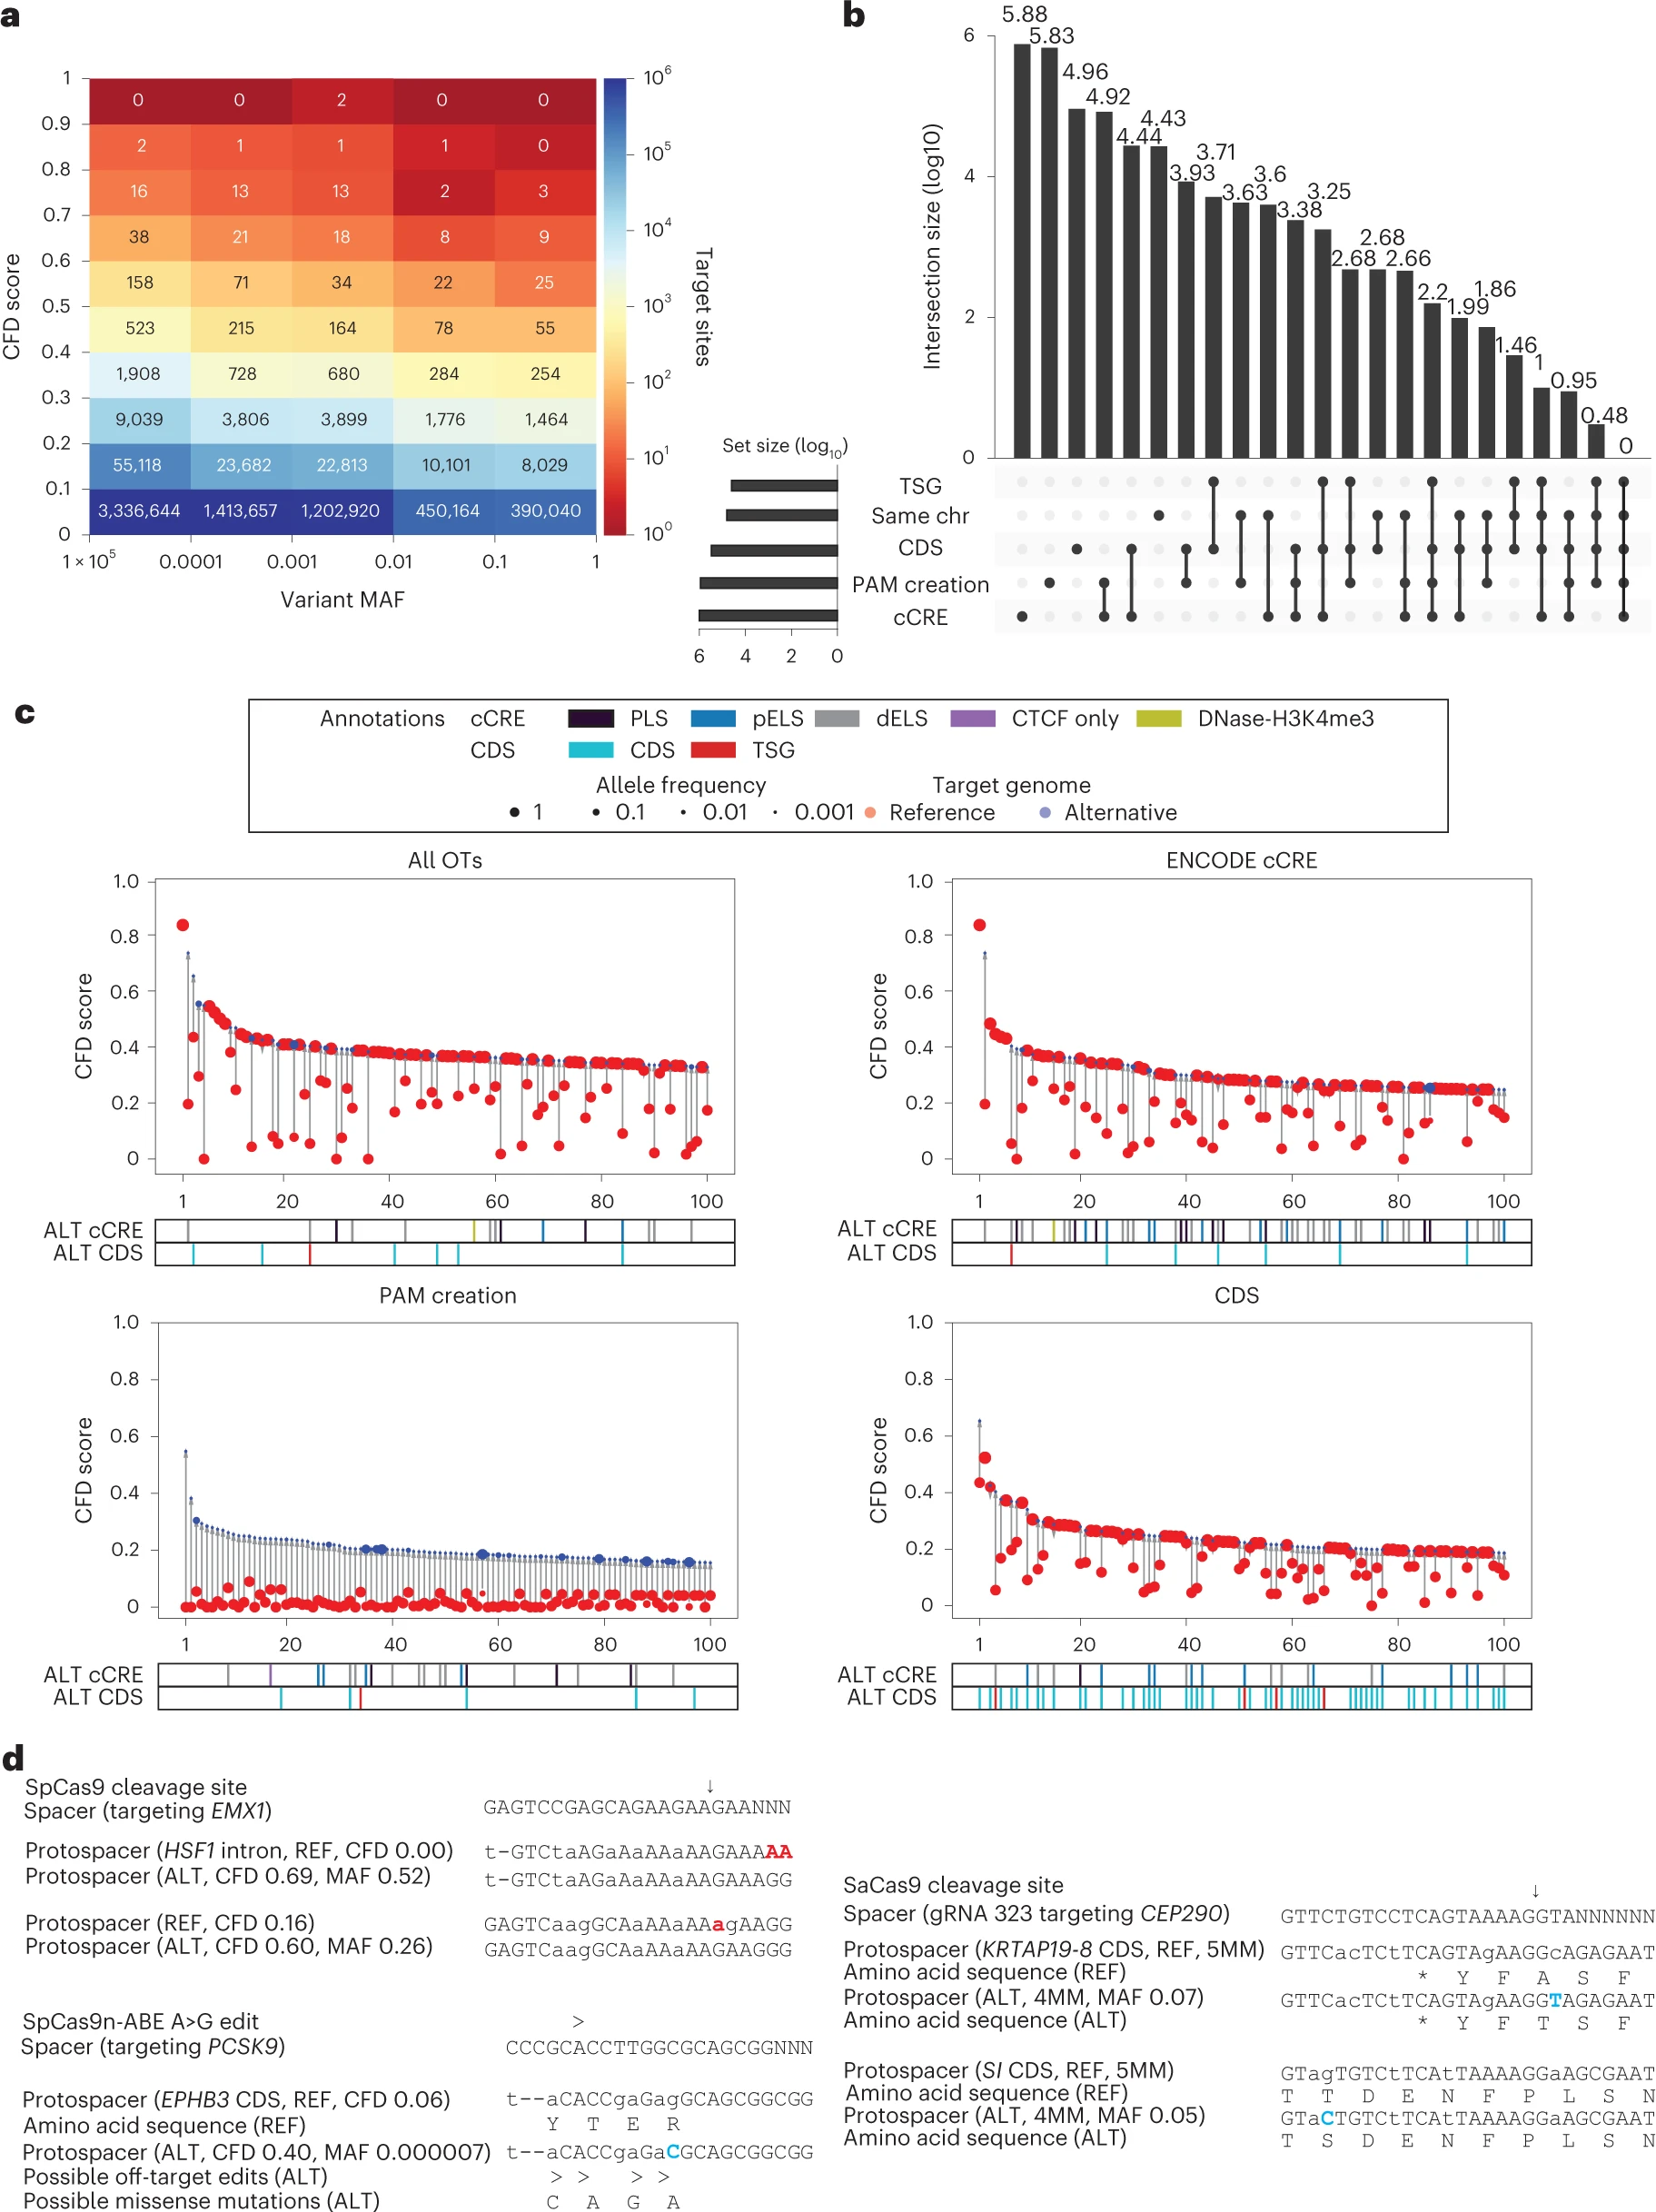
\includegraphics[width=\textwidth]{figures/crisprme8.png}
	\caption[CRISPRme illustrates prevalent off-target potential due to genetic variation]{\textbf{CRISPRme illustrates prevalent off-target potential due to genetic variation (A)} Heatmap showing the distribution of alternative allele nominated off-targets for SpCas9 guides by CFD score and MAF. \textbf{(B)} UpSet plot showing overlapping annotation categories for candidate off-targets (tumor suppressor gene (TSG), candidate off-targets on the same chromosome (chr) as the on-target, CDS regions, cCRE from ENCODE and PAM creation events).  \textbf{(C)} Top 100 predicted off-target sites ranked by CFD score for the gRNA targeting PCSK9 with no filter, found in cCREs, corresponding to PAM creation events, and in CDS regions.\textbf{(D)} Candidate off-target sites with increased predicted cleavage potential introduced by common (MAF 52\% and 26\%) indel variants for a SpCas9 gRNA targeting EMX1 (top left). Candidate off-target cleavage sites within coding sequences with increased homology to a lead gRNA for SaCas9 targeting of CEP290 to treat congenital blindness in current clinical trials due to common SNPs (right). Potential missense mutations in the EPHB3 tumor suppressor resulting from candidate off-target A-to-G base editing by a preclinical lead gRNA targeting PCSK9 to reduce low-density lipoprotein cholesterol levels (bottom). MM denotes mismatches, deletions are shown in red, and SNPs are shown in blue.}
	\label{fig:crisprme8}
\end{figure}
\crisprme can nominate variant off-targets for base editors and evaluate their base editing susceptibility within a user-defined editing window. For a gRNA targeting PCSK9 (ref. 37) that has been used with SpCas9-nickase adenine base editor in vivo in preclinical studies to reduce low-density lipoprotein cholesterol levels, four of the top five candidate off-target sites involve alternative alleles, including one with CFD$_{ref}$ 0.2 and CFD$_{alt}$ 0.75 found in an ENCODE candidate enhancer element. \crisprme nominated a candidate off-target associated with a rare variant (MAF 0.0007\%) that increased the CFD score from 0.06 (REF) to 0.40 (ALT) that would be predicted to produce missense mutations in EPHB3, a putative tumor suppressor gene (\textbf{Fig.\ref{fig:crisprme8}(D)}). The underlying computational challenge that \crisprme addresses extends beyond CRISPR-based applications to other technologies based on nucleic acid sequence recognition. For example, \crisprme can nominate off-targets for RNA-targeting strategies, whether RNA-guided gene editors or even oligonucleotide sequences used as RNA interference or antisense oligo therapies (\textbf{Fig.\ref{fig:crisprme9}}). We performed a variant-aware search (without PAM restriction) for the FDA-approved antisense oligonucleotide Nusinersen \citep{finkel2017nusinersen, mercuri2018nusinersen}, which targets SMN2 pre-mRNA to treat spinal muscular atrophy. Using \crisprme, we identified a potential off-target site within a coding region wherein a common SNP (MAF 2\%) reduces the number of mismatches from three (REF) to two (ALT). Similarly, analysis of the FDA-approved RNA interference therapy Inclisiran \citep{raal2020inclisiran}, which targets PCSK9 mRNA to treat hypercholesterolemia, revealed that its antisense strand has a candidate off-target in the 3' untranslated region of the ribosomal gene RPP14 for which a common insertion variant (MAF 36\%) reduces the number of mismatches and bulges from seven (REF) to four (ALT).
\begin{figure}
	\centering
	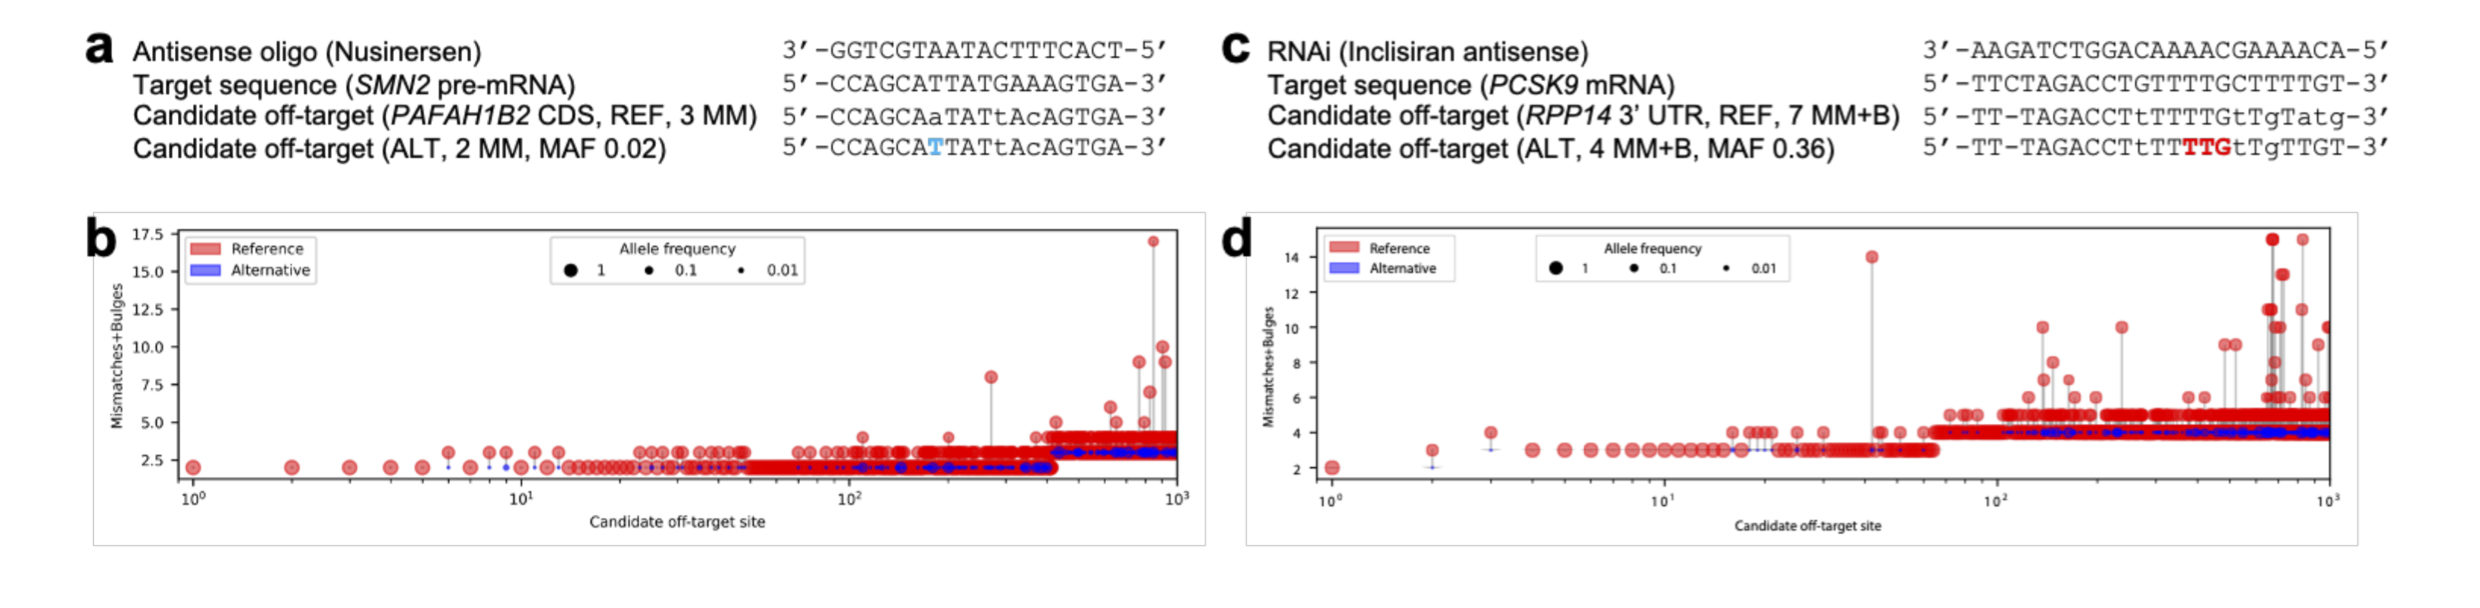
\includegraphics[width=\textwidth]{figures/crisprme9.png}
	\caption[Candidate transcript off-targets introduced by common genetic variants for non-CRISPR sequence-based RNA-targeting therapeutic strategies]{\textbf{Candidate transcript off-targets introduced by common genetic variants for non-CRISPR sequence-based RNA-targeting therapeutic strategies. (A)} A common SNP (in blue) introduces a candidate CDS off-target site with 2 mismatches for the FDA-approved antisense oligo Nusinersen. \textbf{(B)} Top 1000 candidate transcript off-targets ranked by mismatches and bulges for Nusinersen from a search performed with the 1000G and HGDP genetic variant datasets. \textbf{(C)} A common insertion variant (in red) introduces a candidate 3’UTR off-target site with 4 mismatches + bulges for the FDA-approved RNAi therapy Inclisiran. \textbf{(D)} Top 1000 candidate transcript off-targets ranked by mismatches and bulges for Inclisiran from a search performed with the 1000G and HGDP genetic variant datasets.}
	\label{fig:crisprme9}
\end{figure} 
% -- Limitations and Discussion
\subsection{ Limitations and Discussion}
These results demonstrate how personal genetic variation may influence the off-target potential of sequence-based therapies like genome editing. Increased availability of haplotype-resolved genomes of diverse ancestry would enhance ability to nominate variant-associated off-target sites present in human populations. A limitation of current tools including \crisprme is that potential off-targets cannot be enumerated based on structural variants or other complex genetic events such as combinations of indels and SNPs \citep{cancellieri2023human}. Future extensions of CRISPRme based on new data structures such as graph genomes \citep{paten2017genome, garrison2018variation} could enable these complex searches and improve their efficiency. The practical implications of allele-specific off-target editing need to be considered on a case-by-case basis.  In the case of BCL11A enhancer editing, up to $\sim$10\% of SCD patients with African ancestry would be expected to carry at least one rs114518452-C allele, leading to $\sim$10\% cleavage at an off-target site that was not identified in prior studies of this gRNA using currently available tools. Our results highlight that allele-specific off-target editing potential is not equally distributed across all ancestral groups but is especially concentrated in those of African ancestry where genomic variation is most pronounced. Therefore, gene editing efforts that include subjects of African ancestry (like those targeting SCD) might pay particular attention to this issue. Gene editing efforts that focus on a specific patient population should consider genetic variants enriched in that population during off-target evaluation. However, our analysis also shows that variant off-targets may be private to a given individual, so all humans could potentially be susceptible to such an effect. Implementing off-target analysis and testing into therapeutic genome editing protocols in practice is an important issue that is broader in scope than our report. Fundamentally, variant-aware off-target analysis may identify off-target potential that would be overlooked by conventional analysis. Of note, as is true for off-target genetic changes in general, the mere possibility of somatic genetic alteration does not imply functional consequence. Although in principle, ex vivo-edited patient cells could be tested by sequencing before infusion, the functional importance of off-target edits may range from likely functional to likely neutral, so the mere presence of off-target editing in a cell product may not necessarily preclude its clinical use, and this testing could deplete precious material and delay therapy. We recommend several steps to minimize risk of unintended allele-specific off-target effects during therapeutic genome editing, consistent with regulatory guidance to consider effects of genetic variation. First, prioritize use of genome editing methods that maximize specificity, such as high-fidelity editors and pulse delivery. Second, nominate off-targets in a variant-aware manner, with particular attention toward genetic variants found in relevant patient populations, using a tool like \crisprme \citep{cancellieri2023human}. Third, use off-target detection assays that are variant-aware to empirically evaluate the likelihood of off-target editing, although these may imperfectly reflect editing in a therapeutic context (Supplementary Note 7). When possible, allele-specific off-target editing potential should be validated in primary cells of relevant genotype by sequencing. However, it may be difficult to obtain such primary cells to perform biological validation in a relevant therapeutic context. Fourth, perform a risk assessment of variant off-target editing given predicted genomic annotations, mechanisms of DNA repair, delivery to target cells and disease context. For example, off-target edits within tumor suppressor loci might carry greater risk than those targeting unannotated noncoding sequences. Fifth, if excess allele-specific genome editing risks are identified, consider including genotype among the subject inclusion/exclusion criteria. Finally, for therapeutic genome editing indications in which it is feasible (such as hematopoietic cell targeting), prospectively monitor somatic modifications in patient samples to gather information about the frequency and consequence of such events to help assess patient-specific risk and provide valuable information for the broader field as to the frequency and in vivo dynamics of off-target edits if present.\crisprme offers a simple-to-use tool to comprehensively evaluate off-target potential across diverse populations and within individuals. \crisprme is available at \url{http://crisprme.di.univr.it} and may also be deployed locally to preserve privacy.
% ------ Joint genotypic and phenotypic outcome modeling improves base editing variant effect quantification 
\section{Joint genotypic and phenotypic outcome modeling improves base editing variant effect quantification}
Genetic variation contributes substantially to complex disease risk. While well-powered genome-wide association studies (GWAS) \citep{tam2019benefits}and rare variant analyses from cohort studies such as the UK Biobank (UKB) \citep{bycroft2018uk} have associated thousands of loci and genes with clinical phenotypes, these observational approaches are often insufficient to identify causal variants. Perturbation-based methods enable evaluation of the impact of an individual variant in a common genetic background, isolated from genetically linked variants, and such testing can be performed in high throughput through multiplex assays of variant effect (MAVEs) \citep{gasperini2016power}. Numerous types of MAVEs have been developed, including deep mutational scanning (DMS) \citep{araya2011deep},  saturation mutagenesis \citep{myers1986fine}, massively parallel reporter assays (MPRA) \citep{inoue2015decoding},  and CRISPR-based screens \citep{bock2022high, shalem2014genome, wang2014genetic}.  CRISPR base editing screens have emerged as a uniquely powerful method to study variants in their endogenous genomic context. Base editors, fusions of Cas9-nickase and single-stranded cytosine or adenine deaminase enzymes \citep{komor2016programmable, gaudelli2017programmable},enable site-specific installation of transition variants. As the majority of disease-associated variants are single-nucleotide transitions citep{rees2018base}, base editors enable the installation of functionally relevant variants in a precise and scalable way. Base editing screens have been employed to dissect coding variant effects as well as to evaluate GWAS-associated variant functions \citep{hanna2021massively, morris2023discovery, martin2023massively, cuella2021functional, pablo2023scanning, coelho2023base, cheng2021single, sanchez2022base, kim2022high, kweon2020crispr, huang2021identification, sangree2022benchmarking, lue2023base, despres2020perturbing, garcia2023base, lue2023base}. However, base editing efficiency varies substantially depending on the local sequence context surrounding the target base, the specific Cas9 variant and deaminase used, and the cellular context \citep{arbab2020determinants}. Moreover, base edits can occur at multiple positions within the single-stranded DNA bubble created by the guide RNA (gRNA)-DNA binding on the opposite strand, therefore a single gRNA can install a variety of alleles, each with distinct efficiencies. While there have been efforts to predict editing outcomes using massively parallel base editor reporter assay data \citep{arbab2020determinants}, these predictions do not generalize well to unprofiled base editors and cellular contexts \citep{sanchez2022base}. In previous base editing screens, analysis of phenotypic outcomes is confounded by variable editing efficiencies and outcomes. Phenotypic effects of gRNAs with robust editing are exaggerated, and effects of variants that are not installed as efficiently are underestimated. Such confounding is especially pernicious when the target elements are coding variants, as a single gRNA may install distinct coding variants with different frequencies, and current analysis methods are unable to deconvolve such data.  Existing base editing screens have dealt with the heterogeneity in gRNA efficiency and genotypic outcomes in several ways. One approach that has been employed is to assume all editable nucleotides within the editing window are edited with uniform efficiency \citep{hanna2021massively}. Two recent studies have profiled the gRNAs used in phenotypic base editing screening using a base editor reporter (or sensor) assay \citep{sanchez2022base, kim2022high} to filter gRNAs with low editing efficiency when analyzing their phenotypic data. Despite these initial efforts, the computational analyses of these screens have not yet been formalized, often relying on existing tools that were not designed specifically for base editor data with or without the target site reporter. Here, we design an experimental-computational pipeline to improve the accuracy of variant effect estimation in base editing screens. By incorporating a target site reporter sequence into the gRNA construct, we simultaneously measure the editing efficiency of a gRNA and its phenotypic impact. We develop a computational pipeline, BEAN, that normalizes the phenotypic scores of target variants using genotypic outcome information collected from the target site reporter. Moreover, we extend BEAN to analyze densely tiled coding sequence base editing screen data, sharing information among neighboring gRNAs to obtain accurate phenotypic scores for each coding variant. BEAN provides a first-in-class integrated solution to experimental assessment of variant effects through base editing screens. We systematically benchmark BEAN against current state-of-the-art methods for the analyses of pooled CRISPR screens and show substantially improved performance of BEAN. To leverage activity-normalized base editing screening, we have conducted screens assessing the impact of low-density lipoprotein cholesterol (LDL-C)-associated GWAS variants and low-density lipoprotein receptor (LDLR) coding variants on LDL-C uptake in HepG2 hepatocellular carcinoma cells. Genetic differences in LDL-C levels contribute substantially to coronary artery disease risk. Serum LDL-C measurements are quantitative and nearly uniformly measured in most biobanks, and thus they provide among the highest quality human phenotypic data for any trait. A trans-ancestry GWAS meta-analysis from the Global Lipids Genetics Consortium (GLGC) has identified $>$900 genome-wide significant loci associated with blood lipid levels, including $>$400 loci associated with LDL-C \citep{graham2021power}. LDL-C GWAS loci overlap strongly with liver-enriched gene expression, nominating liver as the primary tissue driving LDL-C variant effects \citep{wang2022epic, finucane2018heritability}. Yet, the causal variants and mechanisms by which many of these loci modulate LDL-C levels remain unknown.  LDL-C levels are also impacted by rare coding variants. In the most severe instances, inherited monogenic variants in several genes cause Familial Hypercholesterolemia (FH), a disease associated with extremely elevated LDL-C levels and premature cardiovascular disease \citep{bouhairie2015familial}. The majority of genetic mutations known to cause FH occur in LDLR, a cell surface receptor that uptakes LDL, thus removing it from circulation \citep{brown1984ldl} Despite the effectiveness of lipid lowering therapies, FH patients are still 2-4-fold more likely to have coronary events than the general population \citep{mundal2018impact}. Elevated LDL-C levels increase cardiovascular disease risk throughout life, so the early identification of at-risk individuals would have immense clinical utility \citep{bouhairie2015familial}. However, many LDLR variants currently lack clinical interpretation. Of the 1,427 LDLR missense variants in the ClinVar databasen \citep{landrum2020clinvar}, 50\% are classified as variants of unknown significance (VUS) or to have conflicting interpretations of pathogenicity (“conflicting”), thus impeding FH diagnosis. Likewise, of the 758 unique LDLR missense variants carried by sequenced individuals in the UKB cohort, 69\% are either unreported or have an uncertain annotation in ClinVar. Altogether, improved understanding of LDLR variant impacts would enable earlier diagnosis and treatment for a large number of at-risk individuals. We have modeled the impacts of both common GWAS-associated and rare LDLR coding variants through base editing installation followed by cellular uptake of fluorescent LDL-C in HepG2 cells, which provides a scalable flow cytometric assay to measure a key contributing factor of serum LDL-C levels \citep{hamilton2023systematic} given the majority of serum LDL-C is cleared in liver \citep{spady1992hepatic}.  By applying our experimental-computational pipeline to this screen model, we identify LDL uptake-altering GWAS-associated variants and characterize their downstream impact on chromatin accessibility, transcription factor binding, and gene expression that leads to differential LDL uptake. We nominate causal variants that alter LDL-C uptake through impacting the genes  OPRL1, VTN, and ZNF329, which have not previously been connected with LDL-C levels. Through saturation tiled base editing of LDLR, not only do we accurately distinguish known pathogenic vs. benign variants, we find strong correlation between missense variant functional scores and the LDL-C levels of patients in the UKB who carry these variants. We combine functional scores with structural modeling to mechanistically classify deleterious variant impacts, revealing a key, conserved tyrosine residue in each LDLR class B repeat that interacts with the neighboring repeat to maintain structural integrity. Altogether, BEAN provides a widely applicable tool to characterize single-nucleotide variant functions. 
% ---- A base editing reporter profiles endogenous editing outcomes
\subsection{A base editing reporter profiles endogenous editing outcomes}
\begin{figure}
	\centering
	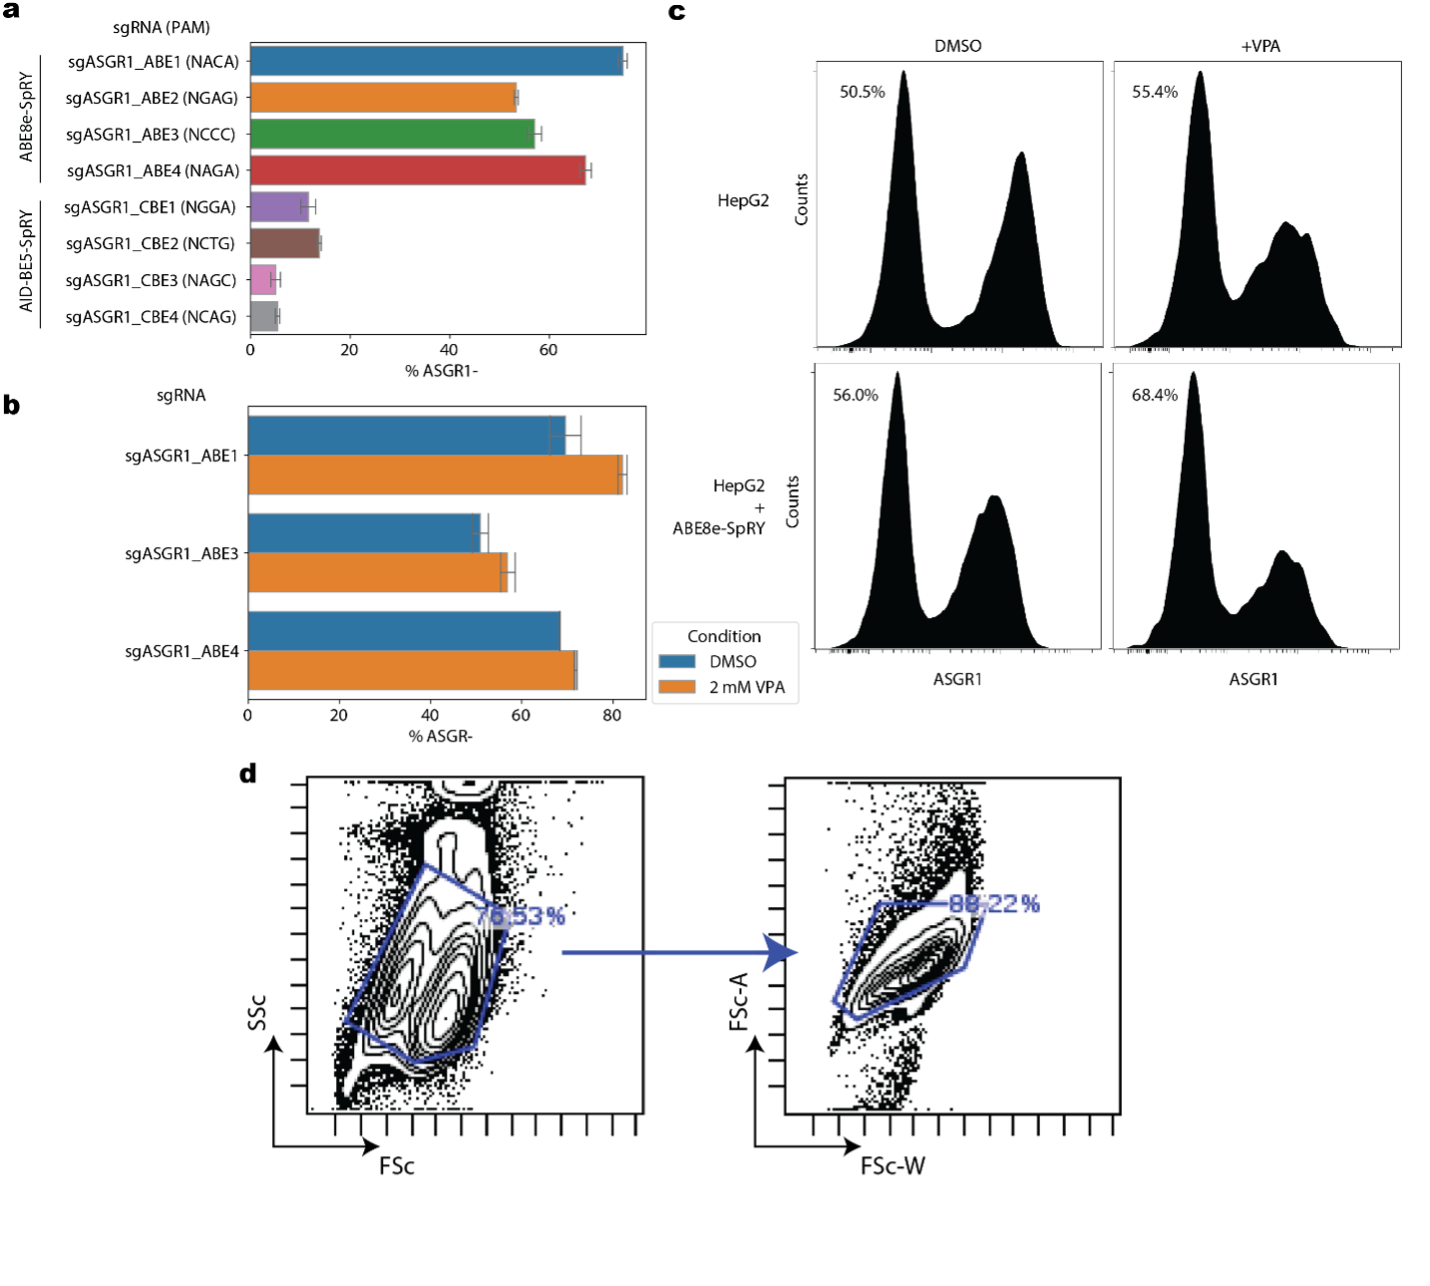
\includegraphics[width=\textwidth]{figures/crisprbean1.png}
	\caption[Optimization of SpRY base editing]{\textbf{Optimization of SpRY base editing. (A)} ) gRNA editing efficiency in HepG2 with ABE8e-SpRY and AID-BE5-SpRY for ASGR1 splice site-targeted gRNAs, measured by the fraction of ASGR1 negative cell counts (\% ASGR -) quantified by flow cytometry from two experimental replicates. \textbf{(B)} gRNA editing efficiency with and without valproic acid (VPA) treatment from 4 experimental replicates. \textbf{(C)} Flow cytometry signal with and without stable ABE8e-SpRY integration and valproic acid (VPA) treatment. Fraction of ASGR negative cell counts in each condition is labeled as percentage in the panel.  \textbf{(D)} Example flow cytometric gates used in all analysis and sorting experiments to filter for single cells. }
	\label{fig:crisprbean1}
\end{figure} 
To enable accurate interrogation of variant effects at scale, we built a platform to perform dense, high-coverage base editing screens that accounts for variable editing efficiency and genotypic outcomes. To maximize coverage of variants in base editing screens, we built lentiviral adenine (ABE8e) \citep{gaudelli2017programmable, richter2020phage} and cytosine (AID-BE5) \citep{arbab2020determinants} deaminase base editor (BE) constructs using the near-PAM-less SpCas9 variant, SpRY \citep{walton2020unconstrained}. Both BEs showed native genomic editing activity, as measured in HepG2 cells by ASGR1 splice site editing followed by flow cytometric anti-ASGR1 antibody staining, with ABE8e-SpRY showing considerably more robust maximal activity (\textbf{Fig.\ref{fig:crisprbean1}(A)}). Editing efficiency was increased by 5-10\% by prior lentiviral integration of constitutively expressed BEs and by transient dosing of cells with the histone deacetylase valproic acid immediately after BE and gRNA transduction (\textbf{Fig.\ref{fig:crisprbean1}(B)-(C)}), and thus these treatments were implemented in all screens.Base editing efficiency is known to vary depending on Cas9 binding efficiency as well as the local sequence and chromatin context surrounding the target base \citep{arbab2020determinants, shin2021small, yang2023hmgn1}, and thus we expected gRNAs to vary substantially in editing efficiency across target sites. To account for this variability, we synthesized and cloned each gRNA paired with a 32-nt reporter sequence comprising the genomic target sequence of that gRNA into lentiviral base editor vectors (\textbf{Fig. \ref{fig:crisprbean2}(A)}), akin to previously published CRISPR mutational outcome reporter constructs \citep{sanchez2022base, kim2022high}. When introduced into cells, the gRNA can edit both its native genomic target site and the adjacent target site (reporter) in the lentiviral vector, which can be read out using next-generation sequencing (NGS). 
\begin{figure}
	\centering
	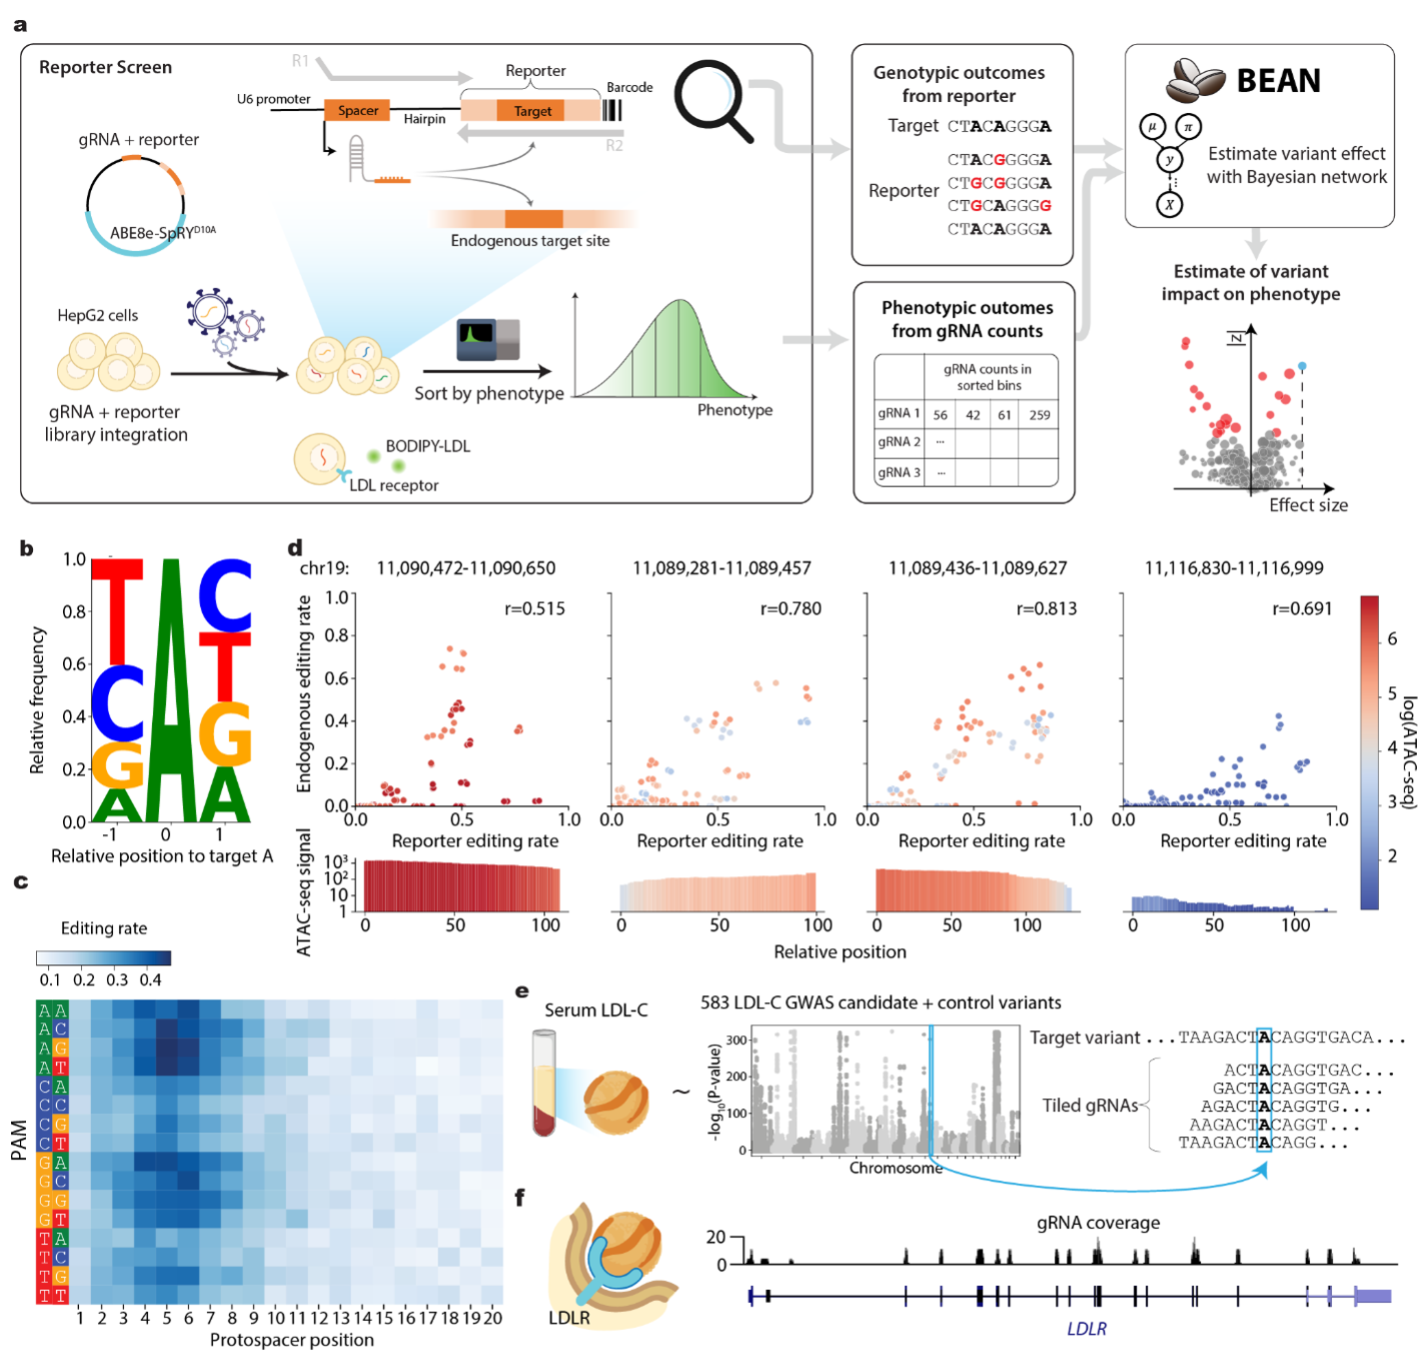
\includegraphics[width=\textwidth]{figures/crisprbean2.png}
	\caption[Activity-normalized base editing screening pipeline]{\textbf{Activity-normalized base editing screening pipeline. (A)} ) Schematic of activity-normalized base editing screening process and analysis by BEAN. A library of gRNAs, each paired with a reporter sequence encompassing its genomic target sequence, is cloned into a lentiviral base editor expression vector. Lentiviral transduction is performed in HepG2, followed by flow cytometric sorting of four populations based on fluorescent LDL-cholesterol (BODIPY-LDL) uptake. The gRNA and reporter sequences are read out by paired-end NGS to obtain gRNA counts and reporter editing outcomes in each flow cytometric bin. BEAN models the reporter editing frequency and allelic outcomes and gRNA enrichments among flow cytometric bins using BEAN to estimate variant phenotypic effect sizes. \textbf{(B)} Adjacent nucleotide specificity of ABE8e-SpRY editing represented as a sequence logo from 7,320 gRNAs; the height of each base represents the relative frequency of observing each base given an edit at position 0.  \textbf{(C)} Average editing efficiency of ABE8e-SpRY by protospacer position and PAM sequence \textbf{(D)} Scatterplots comparing nucleotide-level editing efficiency between the reporter and endogenous target sites for a total of 49 gRNAs across four loci across 3 experimental replicates. The accessibility of the four loci as measured by ATAC-seq signal in HepG2 is shown in the top panel, and the scatterplot markers are colored by the accessibility of each nucleotide. Pearson correlation coefficients are shown as $r$. \textbf{(E)} Schematic of the LDL-C variant library gRNA design for selected GWAS candidate variants with a Manhattan plot showing variant P-values from a recent GWAS study \citep{klimentidis2020phenotypic}.  gRNAs tile the variant at five positions with maximal editing efficiency (protospacer positions 4-8).  \textbf{(F)} gRNA coverage of the LDLR tiling library across LDLR coding sequence along with 5’ and 3’ UTRs and several regulatory regions. }
	\label{fig:crisprbean2}
\end{figure} 
We designed two gRNA libraries using this approach to improve understanding of the genetics of LDL-C levels. The first library (LDL-C GWAS library) targets 583 variants associated with LDL-C levels from the UK Biobank GWAS cohort. We included fine-mapped variants with posterior inclusion probability (PIP) $>$0.25 from either the SUSIE or Polyfun fine-mapping pipelines \citep{wang2020simple, weissbrod2020functionally}, and also variants with PIP $>$ 0.1 within 250 kb of any of 490 genes found to significantly alter LDL-C uptake from recent CRISPR-Cas9 knockout screens \citep{hamilton2023systematic, emmer2021genome}. We designed five tiled gRNAs for each variant allele that place the variant in positions shown to induce most efficient editing with ABE8e (\textbf{Fig. \ref{fig:crisprbean2}(E)}) \citep{arbab2023base}. Positive control gRNAs which ablate splice donor and acceptor consensus sites in six genes found to have significantly altered LDL-C uptake upon knockout \citep{hamilton2023systematic} and 100 non-targeting negative control gRNAs that tile 20 synthetic variants were included, for a total of 3,455 gRNAs.The second library (LDLR tiling library) targeted the LDLR gene. Taking advantage of the flexible PAM recognition of SpRY, every possible gRNA targeting the LDLR coding sequence on both strands was included. Lower density gRNAs, tiled every 2-3-nt, targeted the the 50-nt flanking each LDLR exon, the LDLR 5’ and 3’ UTR, promoter, and two intronic enhancers (\textbf{Fig. \ref{fig:crisprbean2}(F)}). This library also contained 150 non-targeting negative control gRNAs, for a total of 7,500 gRNAs.We first assessed editing outcomes through lentiviral transduction of each library in HepG2 cells followed by NGS of gRNA-reporter pairs 10-14 days afterwards. We developed an end-to-end computational toolkit for base-editing screens, BEAN, which includes the ability to perform quality control and quantify editing outcomes from raw reads among other functionalities. Importantly, the quantification step is designed to account for self-editing of the spacer sequence, which we found to occur at appreciable frequency and with modest correlation with reporter editing frequency (LDL-C GWAS library median 31\%, Pearson $r$=0.36, LDLR tiling library median 18\%, $r$=0.31). We used BEAN to profile the previously uncharacterized PAM-less base editors ABE8e-SpRY and AID-BE5-SpRY on reporter data from the $>$10,000 gRNAs in both libraries (\textbf{Fig.\ref{fig:crisprbean2}(B)} and \textbf{(C)}),. The result clearly recapitulated the hallmark positional preferences of these base editors \citep{myers1986fine, wang2014genetic} the NRY PAM preference of the SpRY enzyme \citep{komor2016programmable, gaudelli2017programmable}, and the relative depletion of editing at AA dinucleotides by ABE8e. Notably, the average maximal positional ABE8e-SpRY editing frequency at protospacer positions 3-8 across dinucleotide PAM sequences ranges from 32\% to 46\%, indicating the ability of this enzyme to install variants efficiently across a wide variety of genomic locations.To validate that editing of the reporter provides an accurate surrogate for endogenous editing, we generated a library where both the reporter and endogenous target site are sequenced following the editing by 49 gRNAs across four loci surrounding LDLR with varying levels of HepG2 chromatin accessibility. We demonstrate that nucleotide-level and allele-level reporter editing fractions correlate well with endogenous target site editing fractions ((\textbf{Fig.\ref{fig:crisprbean2}(D)}, average Pearson correlation across 4 loci is $r$=0.70 for per-nucleotide editing rate $r$=0.70, per-allele editing rate $r$=0.69), and the reporter shows higher correspondence than BE-Hive predictions29 (Nucleotide $r$=0.44, allele $r$=0.64) (\textbf{Fig.\ref{fig:crisprbean3}}). Notably, while reporter editing correlates with endogenous editing at all four loci, we found that endogenous editing frequency also depends on the accessibility of the target region, as has been previously reported for Cas9-nuclease \citep{schep2021impact, ding2019improving, liu2019modulating} and base editors \citep{shin2021small, yang2023hmgn1}. Yet, current computational analyses do not model these dependencies, motivating the development of a tailored modeling framework.
\begin{figure}
	\centering
	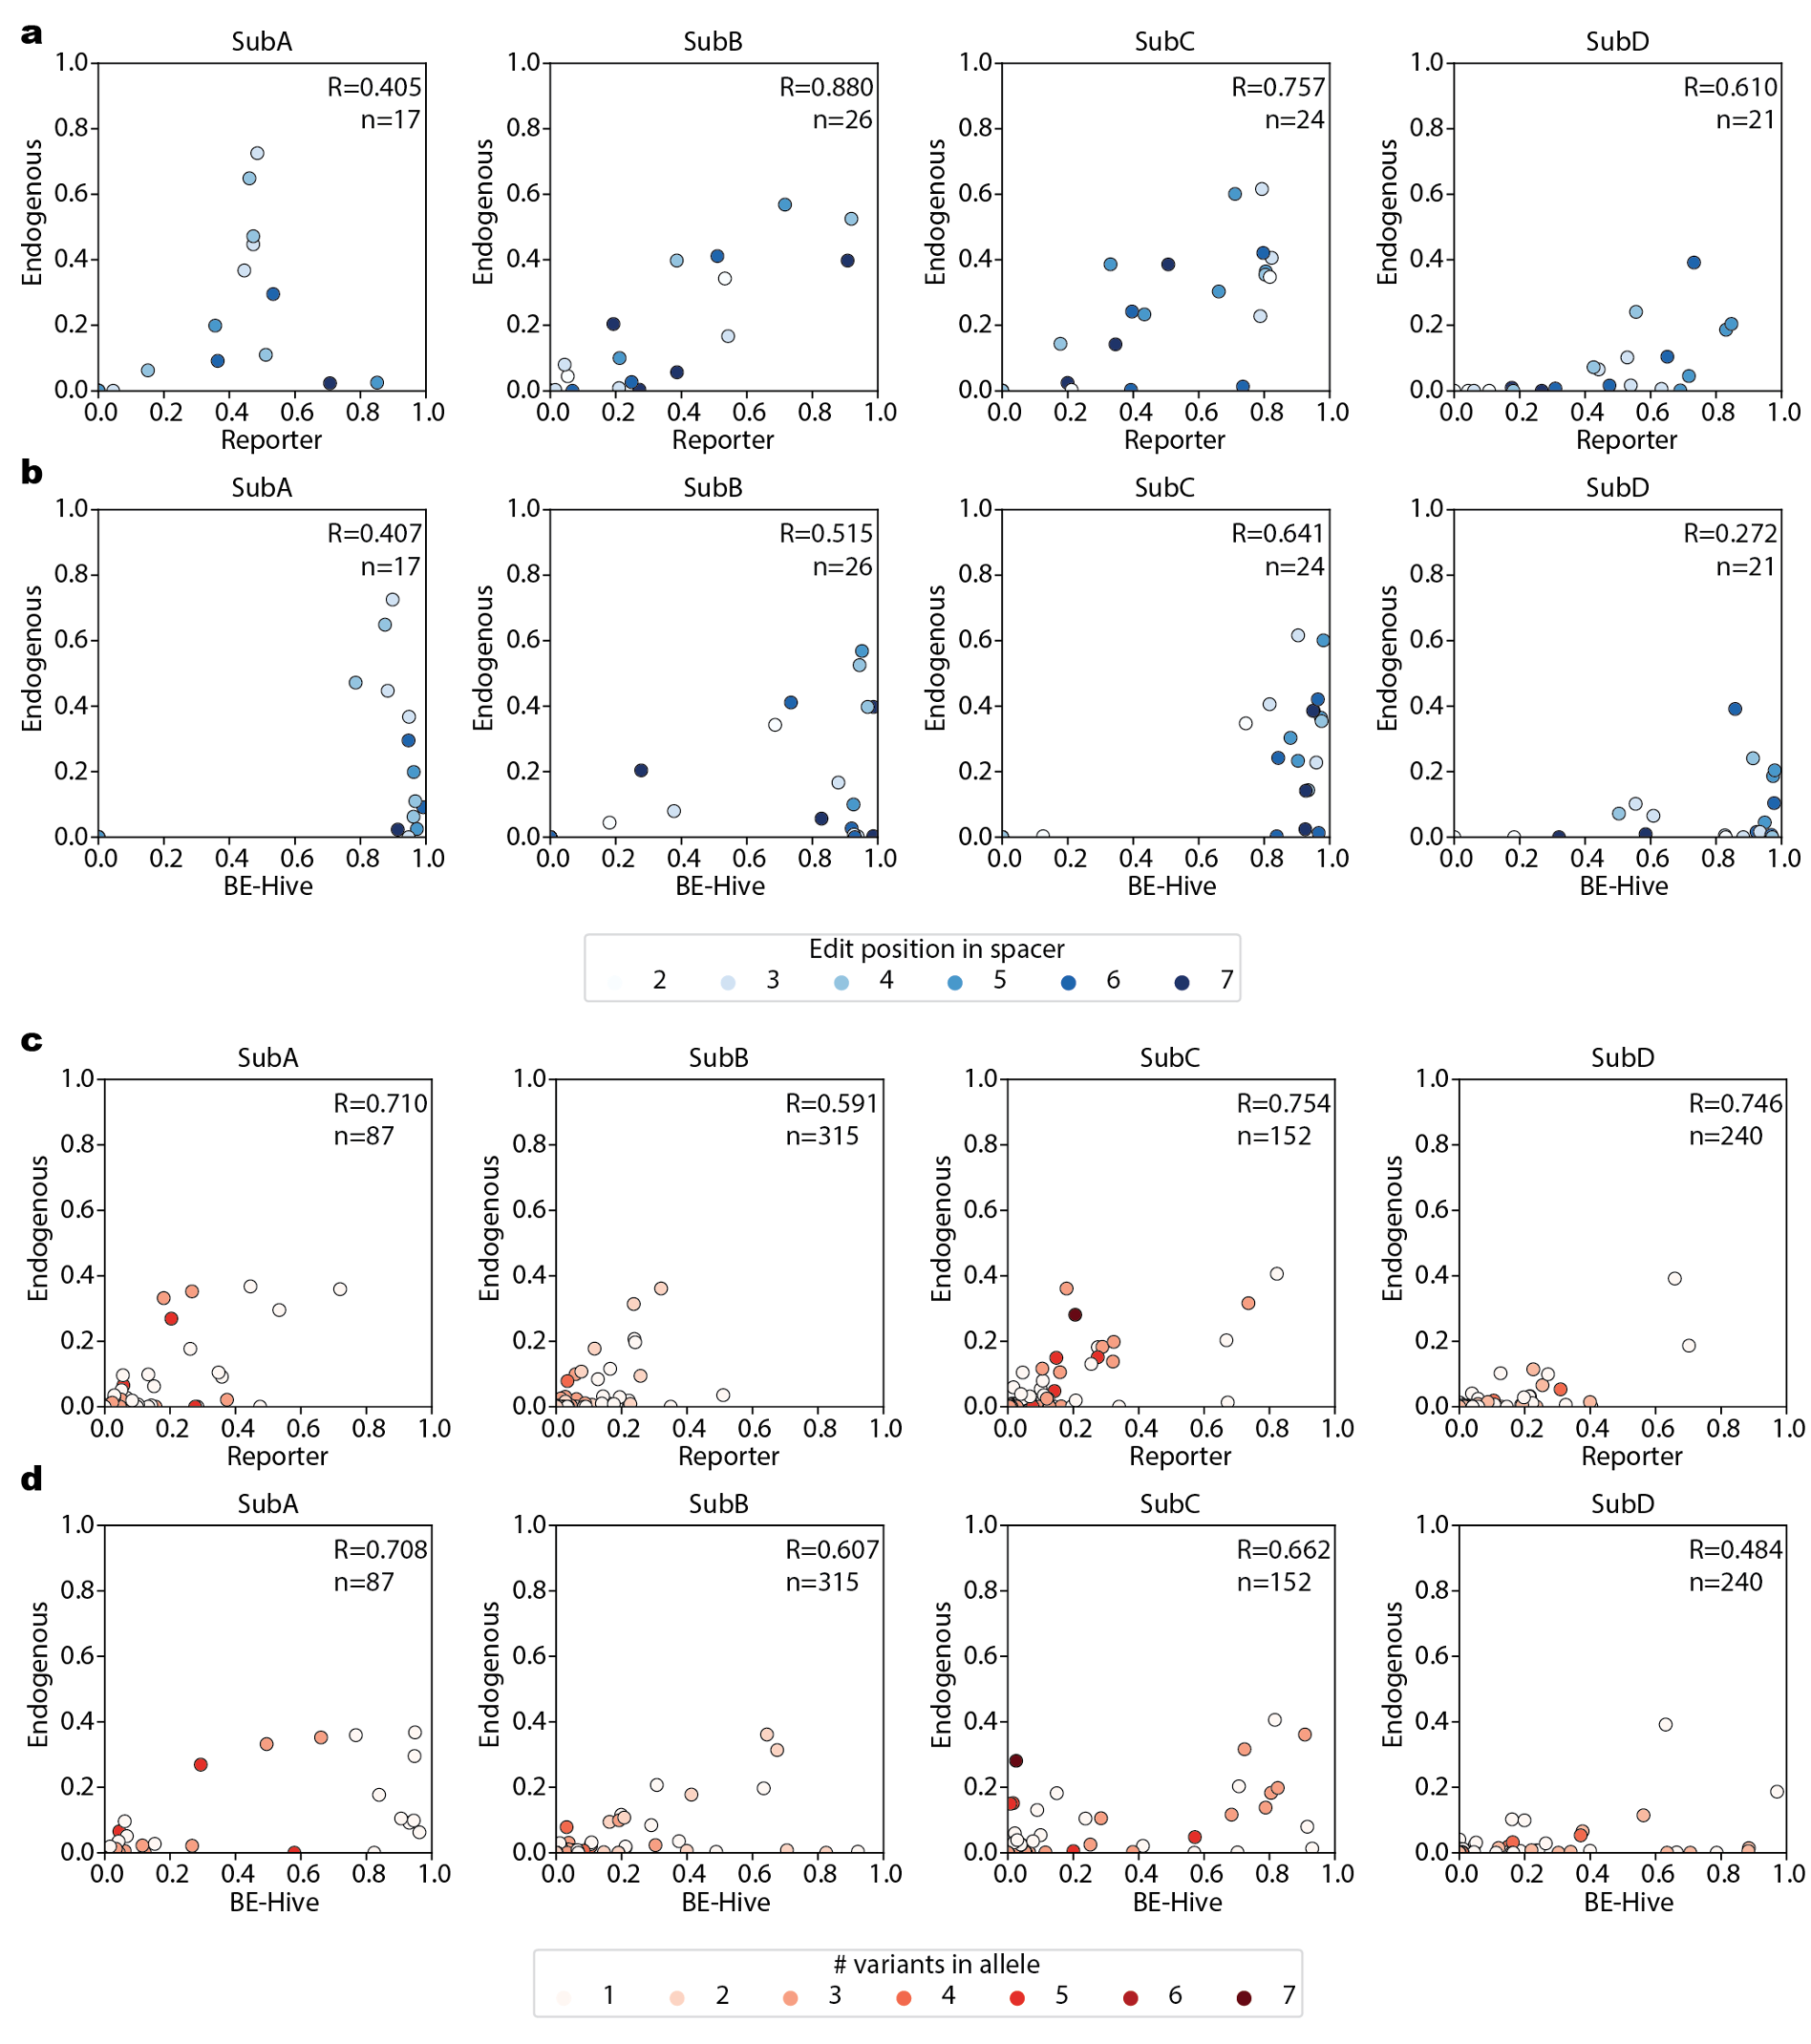
\includegraphics[width=\textwidth]{figures/crisprbean3.png}
	\caption[Endogenous target site editing rate comparison with reporter and BE-Hive predicted editing outcomes]{\textbf{Endogenous target site editing rate comparison with reporter and BE-Hive predicted editing outcomes. } Mean endogenous and reporter edit rates across three replicates are plotted. \textbf{(A)-(B)} Nucleotide-level editing rates in \textbf{(A)} reporter and \textbf{(B)} BE-Hive plotted against those in endogenous loci within protospacer position 2 to 7 (1-based, inclusive). \textbf{(B)} Allele level editing rates in \textbf{(C)} reporter and \textbf{(D)} BE-Hive plotted against those in endogenous loci. Alleles are defined within editing window within protospacer 1 to 19 (1-based, inclusive). SubA-D denotes sublibraries A-D. Pearson correlation coefficients are denoted as R and the number of points is denoted as n.}
	\label{fig:crisprbean3}
\end{figure} 
We then performed fluorescent LDL uptake screens with each library in $\geq$ 5 biological replicates, ensuring $>$500 cells per gRNA at all stages. We used simulation to determine the optimal flow cytometric sorting scheme, accounting for variability in gRNA editing rate, gRNA coverage, gDNA sampling and PCR amplification (\url{https://github.com/pinellolab/screen-simulation}). Based on our simulation result that finer bin widths improves sensitivity (Supplementary Fig. 6, Supplementary Note 1), we flow cytometrically isolated four populations per replicate with the very low (0-20\% percentile), low (20-40\%), high (60-80\%), and very high (80-100\%) LDL uptake (\textbf{Fig.\ref{fig:crisprbean2}(A)}), performing NGS on gRNA and reporter pairs in each sorted population. We observed robust replicability (median Spearman $\rho$=0.84 for LDL-C GWAS library, 0.88 for LDLR tiling library) in gRNA counts across replicates (Supplementary Fig. 7), indicating technical reproducibility.  the variant at five positions with maximal editing efficiency (protospacer positions 4-8). f) gRNA coverage of the LDLR tiling library across LDLR coding sequence along with 5’ and 3’ UTRs and several regulatory regions. 
\begin{figure}
	\centering
	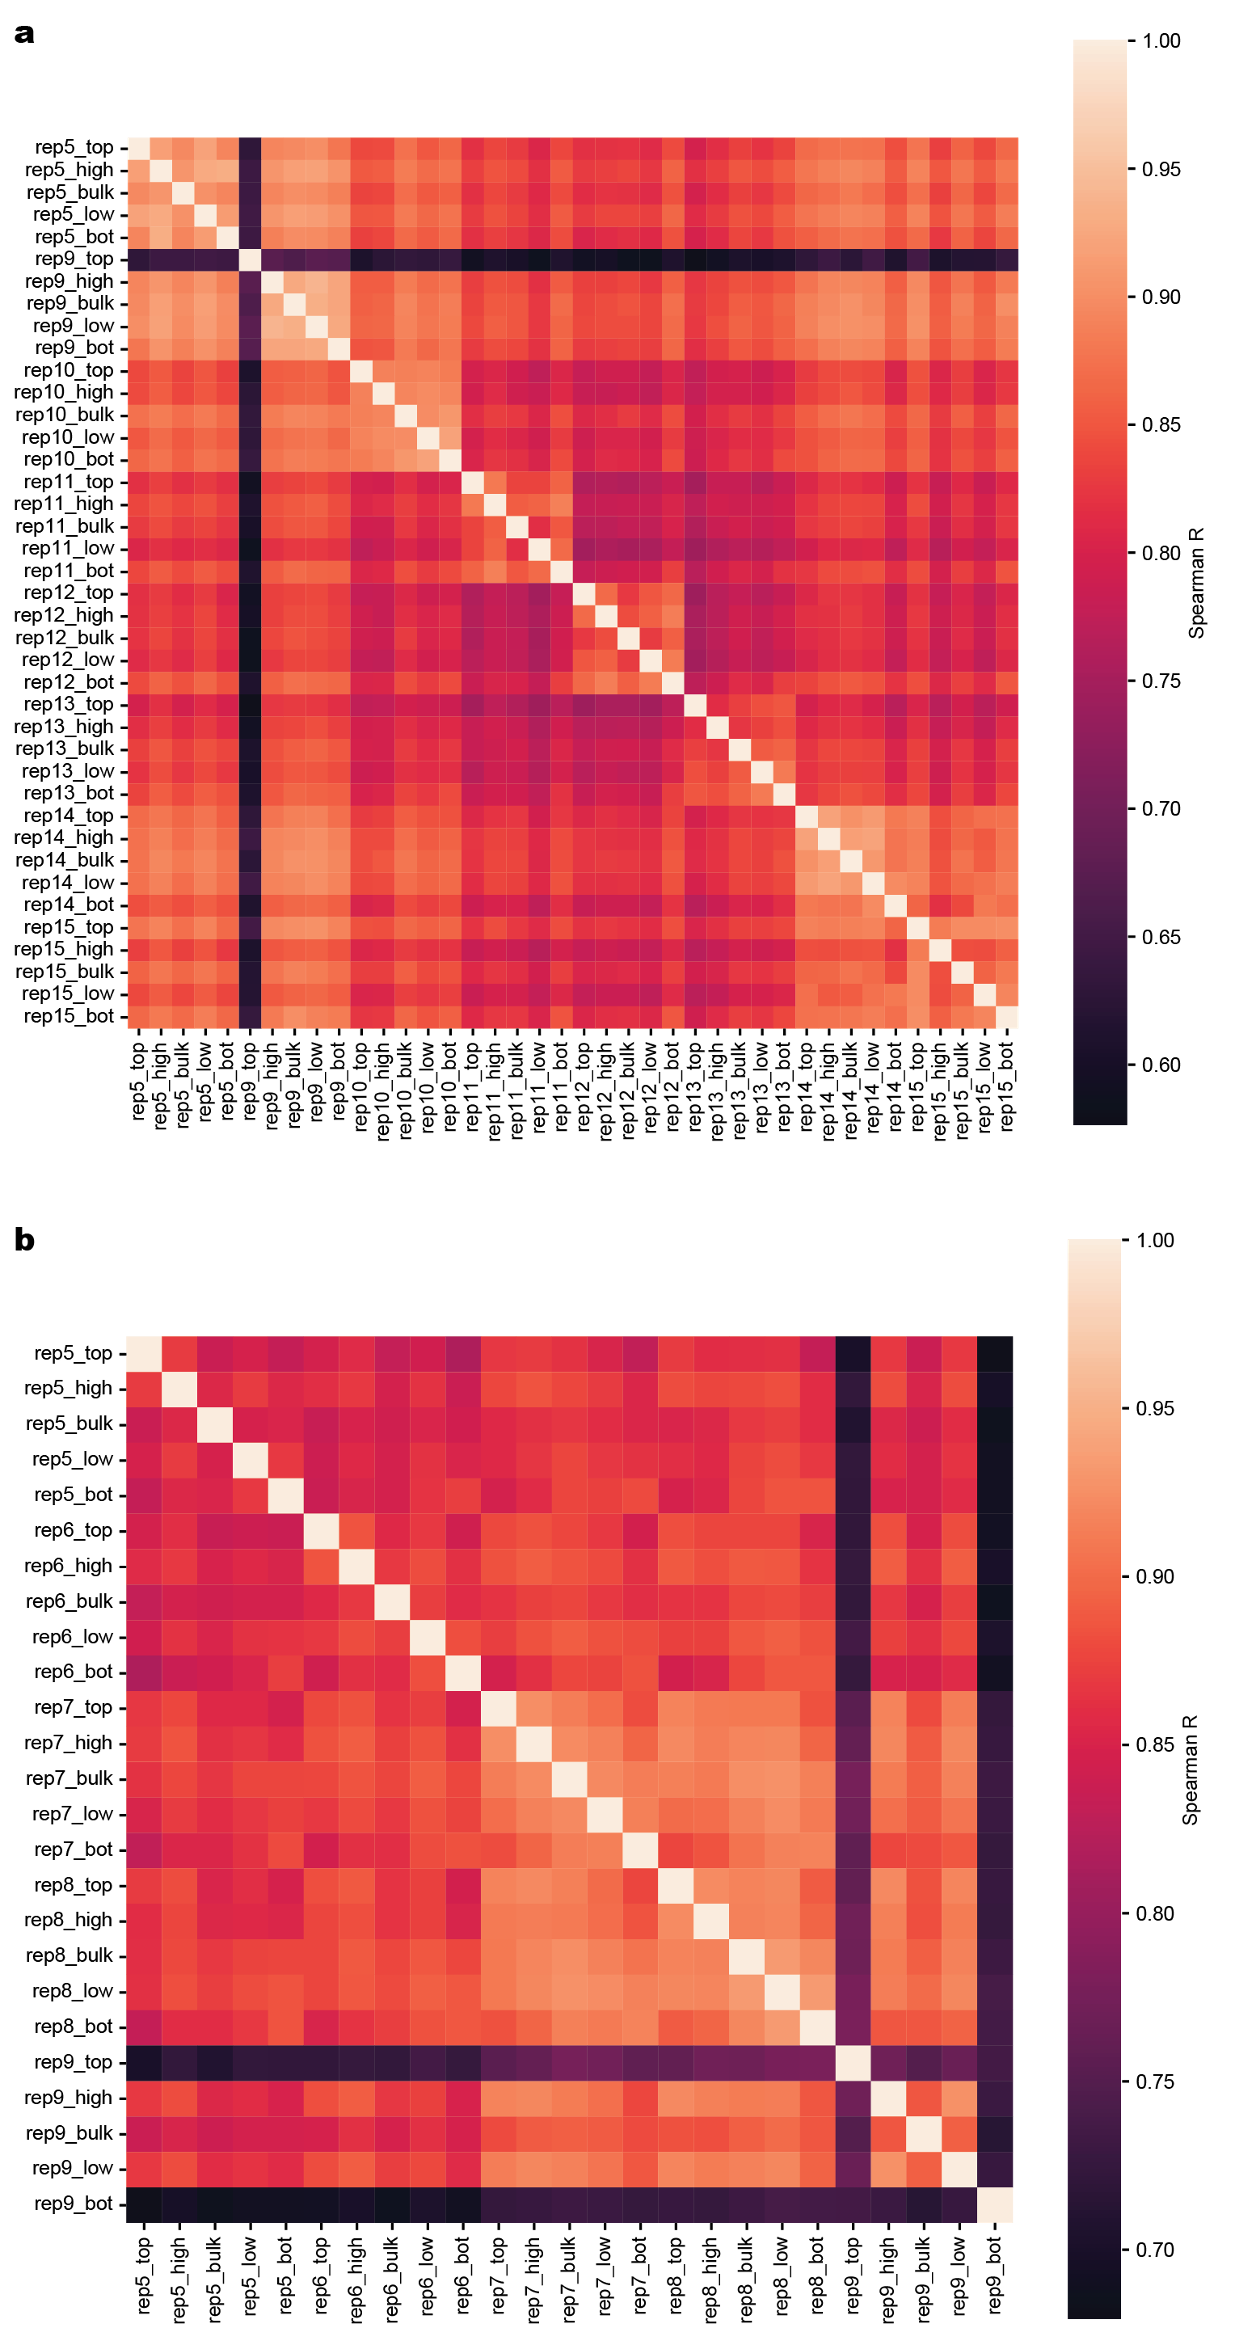
\includegraphics[scale=0.9]{figures/crisprbean4.png}
	\caption[Base editing screen read correlations]{\textbf{Base editing screen read correlations. } Spearman correlation coefficient of \textbf{(A)} gRNA counts of LDL-C GWAS library and \textbf{(B)} LDLR tiling library samples after filtering out for gRNAs with less than 10 read counts. Top; 80-100\%, high; 60-80\%, low; 20-40\%, bot: 0-20\% percentile LDL-C uptake. Rep; experimental replicate.}
	\label{fig:crisprbean4}
\end{figure} 
% -- Activity-normalized base editing screen analysis with BEAN
\subsection{Activity-normalized base editing screen analysis with BEAN}
We postulated that the gRNA editing outcomes provided by the reporter together with the accessibility of the target region could improve the quantification of variant phenotypic effects in our pooled BE screens. To do so, we developed a novel analysis method, BEAN (Base Editor screen analysis with Activity Normalization), to quantify the effect of each variant from gRNA abundance in sorted populations along with genotypic outcome information provided by reporter editing. BEAN assumes that the observed phenotypic distribution in a population of cells for each gRNA derives from a mixture of cells with unedited and edited alleles (\textbf{Fig. \ref{fig:crisprbean5}}). The proportion of cells carrying a given gRNA that possess a particular genotype is inferred based on the editing outcome observed in reporter as well as chromatin accessibility of the target locus using a Bayesian network. The distribution of cells with each gRNA prior to sorting is modeled as a Gaussian mixture for each underlying genotype produced by that gRNA. Because multiple gRNAs may induce the same genotypic outcome at different frequencies, BEAN uses this redundancy to build confidence in the predicted phenotypic impacts of a given genotype. As the output for each variant, BEAN provides its effect size i.e. the posterior mean phenotypic shift along with the corresponding $z$-score, and 95\% credible interval (CI). We also note that BEAN can be adapted to an arbitrary number and arrangement of sorting bins and other base editing enzymes including those with uncharacterized editing preferences, and can accommodate screens without reporter or accessibility information. 
\begin{figure}
	\centering
	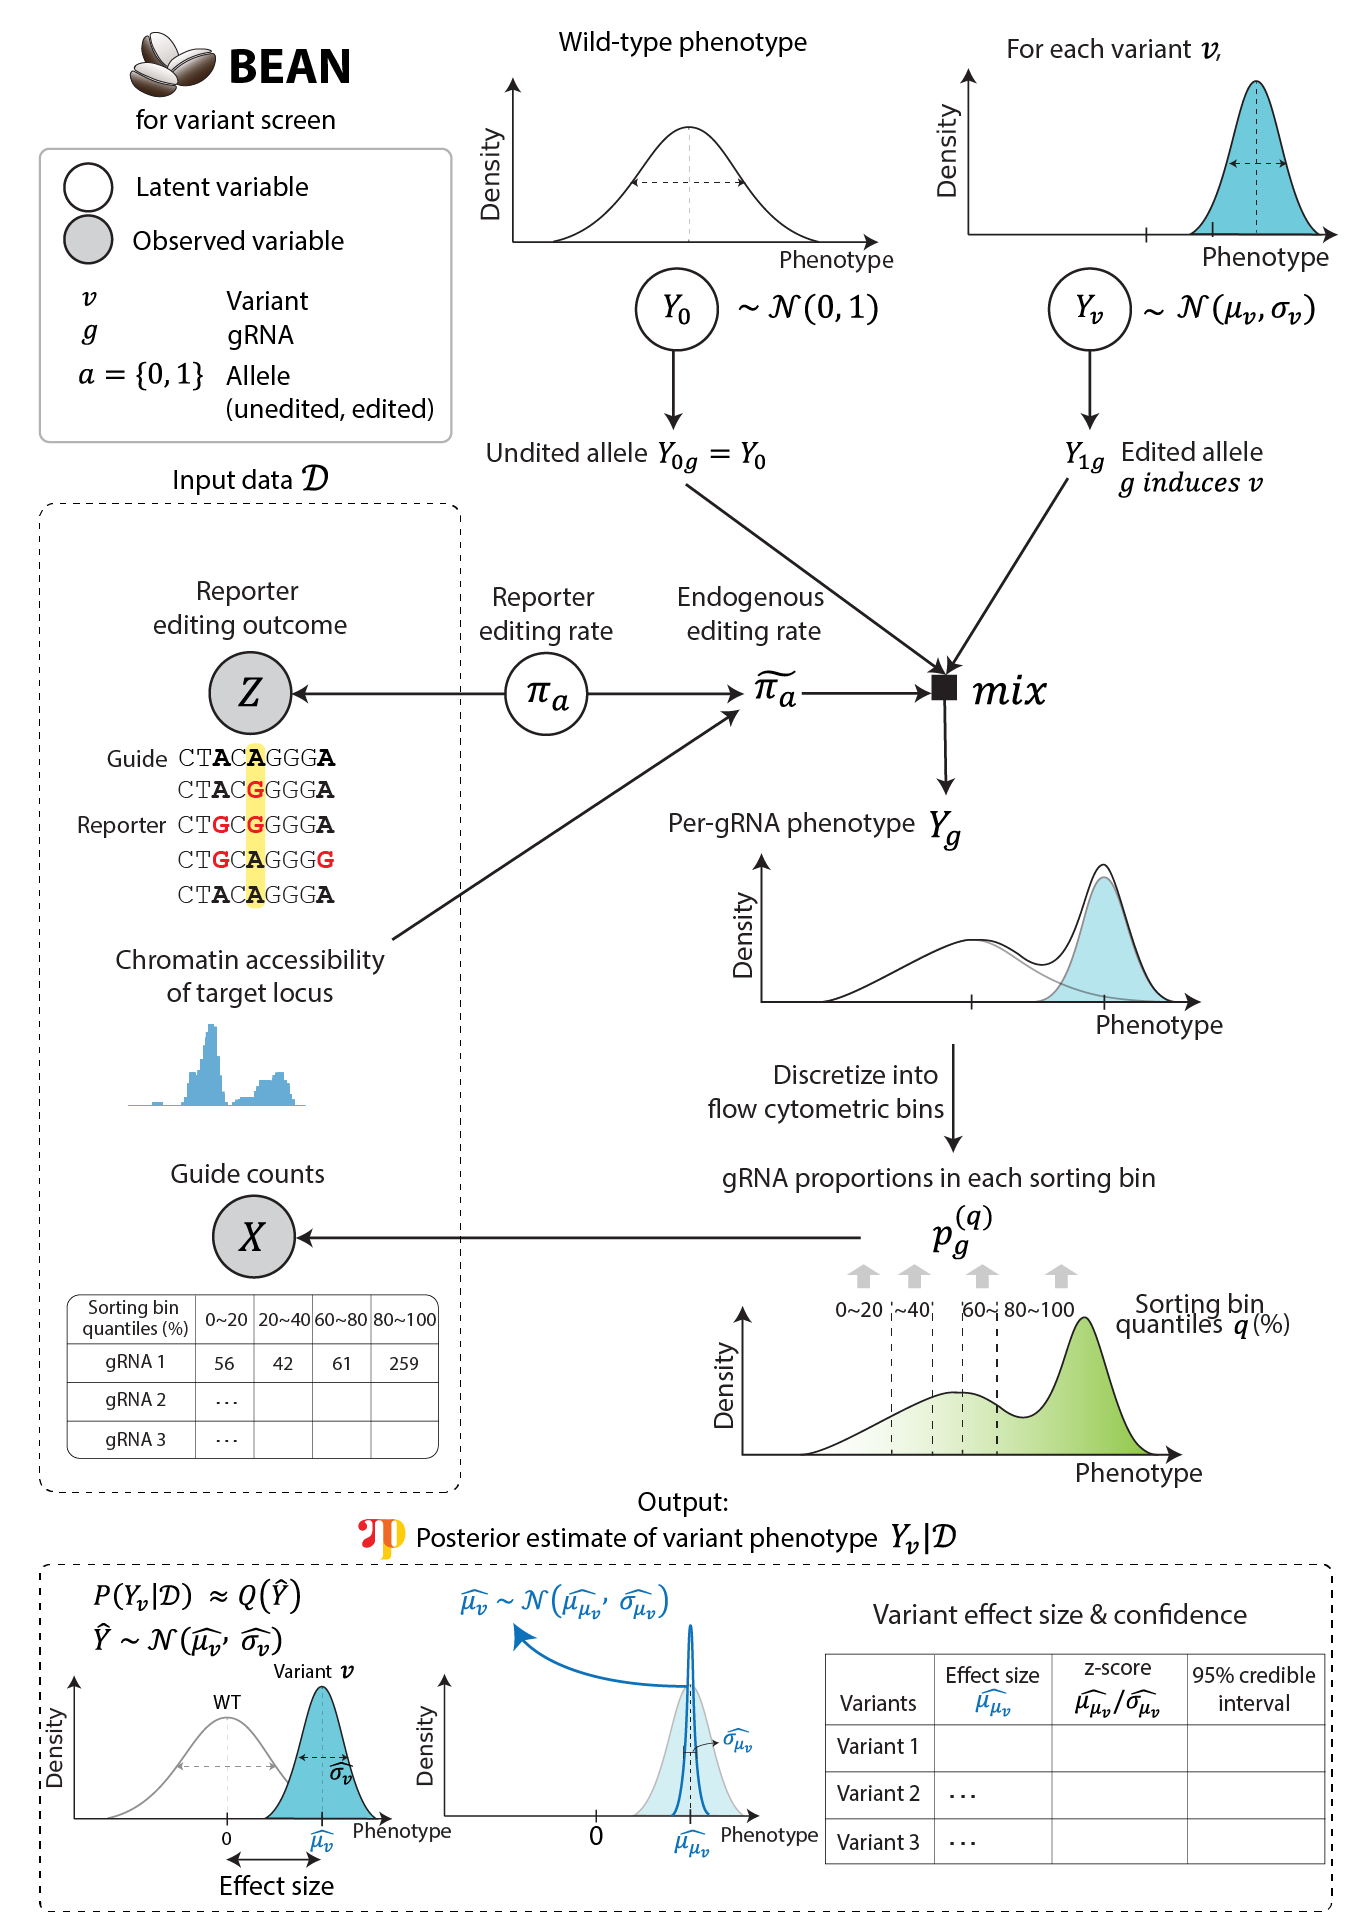
\includegraphics[width=\textwidth]{figures/crisprbean5.png}
	\caption[BEAN models variant effects from activity-normalized base editing screens]{\textbf{BEAN models variant effects from activity-normalized base editing screens. } Simplified schematic of BEAN Bayesian network that models input reporter editing outcomes and gRNA counts. The Bayesian network model recapitulates the data generation process starting from a variant-level phenotype Y$_{v}$ and models per-gRNA phenotypes as a Gaussian mixture distribution of edited and unedited (wild-type) allele phenotypes. The weights of the mixture components are modeled to generate reporter editing outcomes. gRNA abundance in each sorting bin is then calculated by discretizing the gRNA phenotype based on the experimental design into the phenotypic quantiles, and is modeled to generate the observed gRNA counts using an overdispersed multivariate count distribution (see Methods). BEAN outputs the parameters of the posterior distribution of mean phenotypic shift as Gaussian distribution with mean $\hat{\mu_{\mu}}$ (effect size), along with negative-control adjusted $z$-score  and credible interval (CI), where $\mathcal{D}$ is the input data.}
	\label{fig:crisprbean5}
\end{figure} 

BEAN only assumes population-level consistency between editing of the reporter and endogenous target site. We hypothesized that variation in editor expression or cellular state may lead certain cells to be more amenable to editing than others. In this scenario, “jackpot” cells would be more likely to have editing at both endogenous and reporter loci. To assess this possibility, we compared the enrichment of a gRNA in the highest vs. lowest sorted LDL uptake quantile bin with the difference in reporter editing observed in cells sorted into these bins, reasoning that endogenous editing should be highest in the cells sorted into the enriched bin. We indeed observed such correlation for LDLR and MYLIP splice-ablating gRNAs (Spearman $\rho$=0.32, \textbf{Fig. \ref{fig:crisprbean6}}), suggesting the existence of cell-level factors leading to “jackpot” cells with higher editing at both endogenous and reporter loci. However, the correlation between phenotypic and reporter editing enrichment was weaker when considering all positive control gRNAs (Spearman $\rho$=0.13). We thus concluded that incorporating the jackpot effect into BEAN would be unlikely to improve model performance.
\begin{figure}
	\centering
	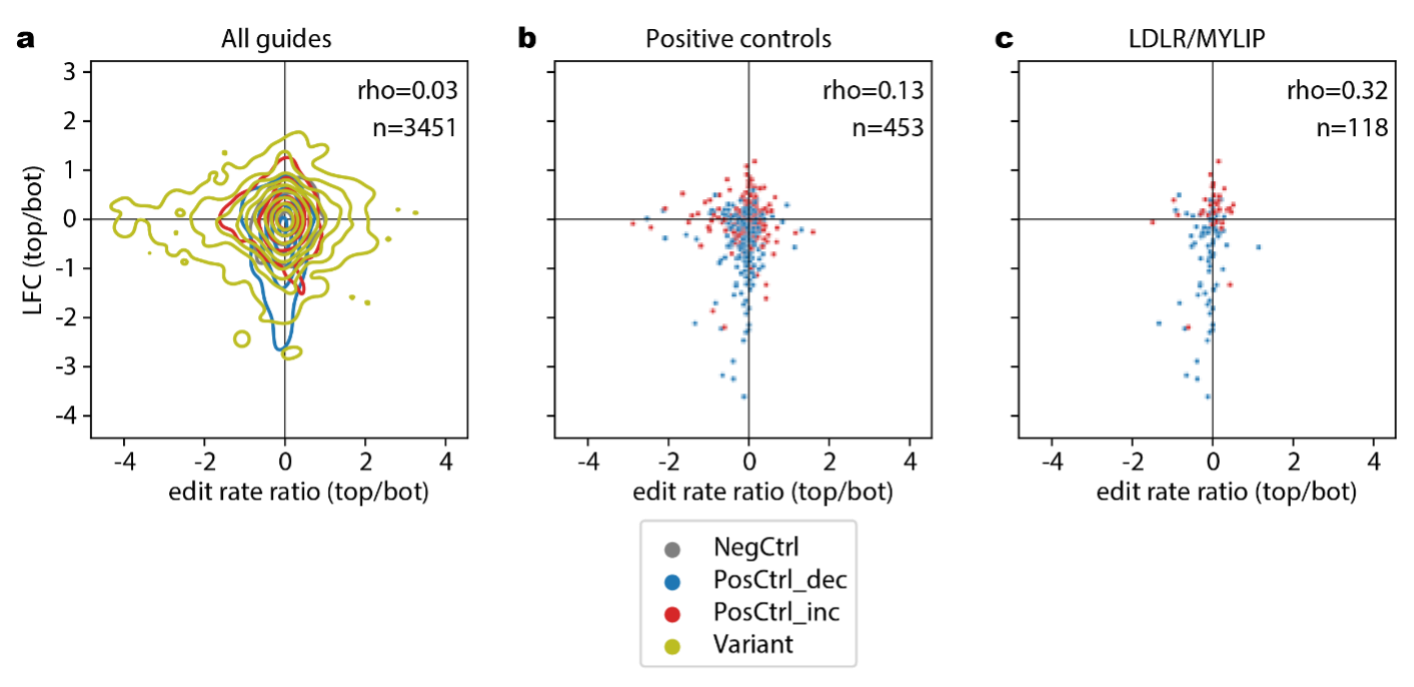
\includegraphics[width=\textwidth]{figures/crisprbean6.png}
	\caption[Jackpot analysis]{\textbf{Jackpot analysis. } Scatterplots of editing rate enrichment plotted against gRNA abundance enrichment of \textbf{(A)} all gRNAs, \textbf{(B)} positive control gRNAs, \textbf{(C)} strongest positive control gRNAs targeting LDLR or MYLIP splicing sites. Enrichment of both editing efficiencies and gRNA abundance is calculated as the log fold chance of the measures in the highest and lowest 20\% quantile bin. Spearman correlation coefficients are shown as rho. NegCtrl; negative control gRNAs, PosCtrl\_dec; positive control gRNAs that is expected to decrease LDL-C uptake, PosCtrl\_inc; positive control gRNAs that is expected to increase LDL-C uptake.}
	\label{fig:crisprbean6}
\end{figure} 
% -- BEAN identifies LDL uptake altering GWAS variants
\subsection{BEAN identifies LDL uptake altering GWAS variants}
We applied BEAN to the LDL-C GWAS library screen. From the reporter data, variant editing efficiency per gRNA is highly variable with average edit fraction of 34.0\%. Encouragingly, most target variants are edited at high efficiency by at least one of the five targeting gRNAs (median maximal editing of 60.4\%, \textbf{Fig. \ref{fig:crisprbean7}}). 
\begin{figure}
	\centering
	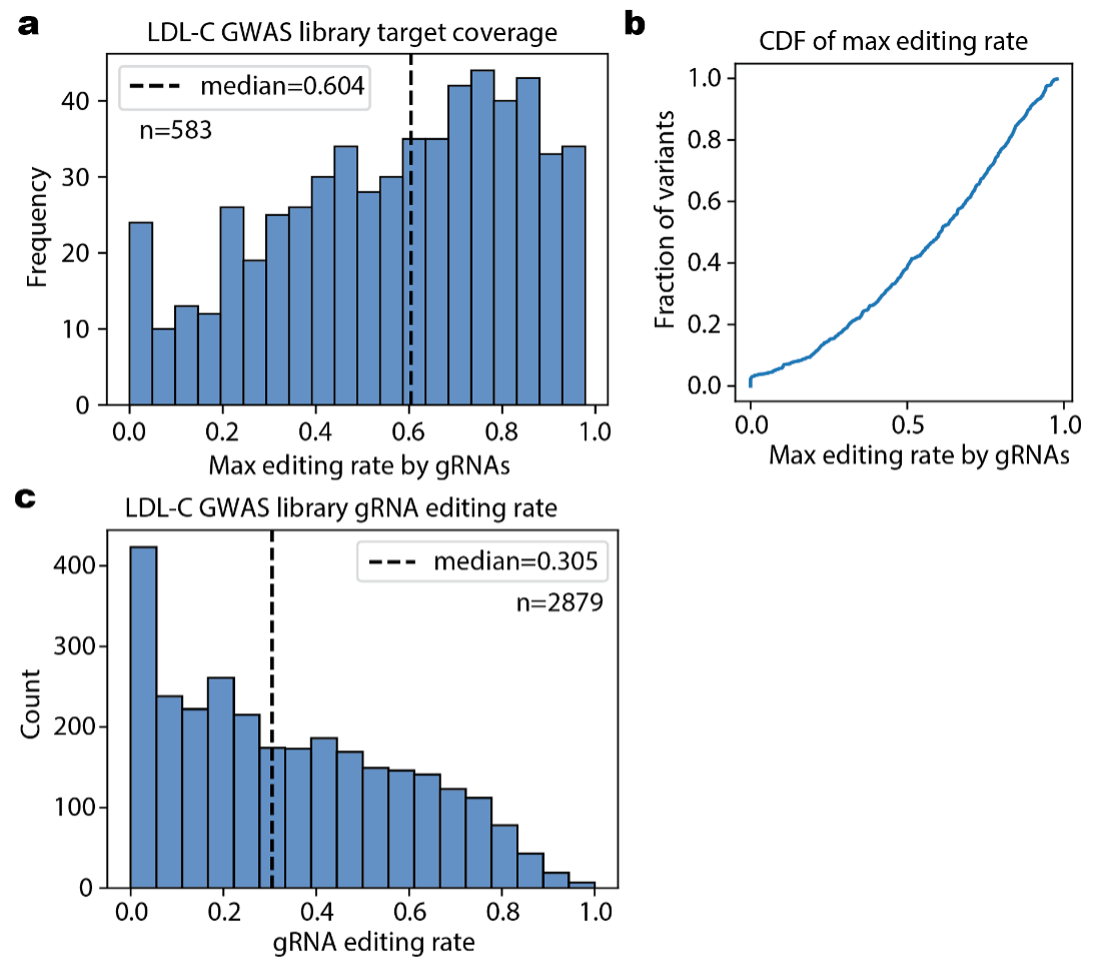
\includegraphics[width=\textwidth]{figures/crisprbean7.png}
	\caption[LDL-C GWAS variant editing coverage]{\textbf{LDL-C GWAS variant editing coverage.} \textbf{(A)} Histogram of per-target variant coverage calculated by the maximal editing rate of the variant by any gRNAs targeting the variant, where gRNA editing rates are calculated as the mean editing rate in bulk samples across replicates where more than 10 reads are observed. \textbf{(B)} Cumulative distribution function of the same distribution plotted in \textbf{(A)}. \textbf{(C)} Per-gRNA editing rate of the target variant in bulk samples across replicates where more than 10 reads are observed. }
	\label{fig:crisprbean7}
\end{figure} 
First, we compared the performance of BEAN and five published CRISPR screen analysis methods at distinguishing the effects of positive control splice-altering variants versus negative control non-targeting gRNAs \citep{huang2021identification, li2014mageck, li2015quality, jeong2019beta, daley2018crisphiermix}  \textbf{Fig. \ref{fig:crisprbean8}(A)}). To dissect the contributions of individual features to BEAN performance, we included two reduced versions of BEAN: one that considers reporter editing but not chromatin accessibility (BEAN-Reporter), and another that ignores the reporter, assuming uniform gRNA editing efficiency (BEAN-Uniform). BEAN outperforms other evaluated methods at this classification task (\textbf{Fig. \ref{fig:crisprbean8}(B)})), and this improved performance is accentuated when the data is subsampled for fewer replicates, demonstrating its ability to maintain robustness even with less data. Importantly, BEAN shows improved performance (mean AUPRC=0.90 across 15 2-replicate subsamples) over BEAN-Reporter (mean AUPRC=0.87), which in turn outperforms BEAN-Uniform (mean AUPRC=0.85), supporting the value of accurately modeling target site editing. Intriguingly, even BEAN-Uniform outperforms alternative approaches, likely due to more accurate modeling of sorting bins, suggesting the utility of BEAN in sorting screens without reporter.
\begin{figure}
	\centering
	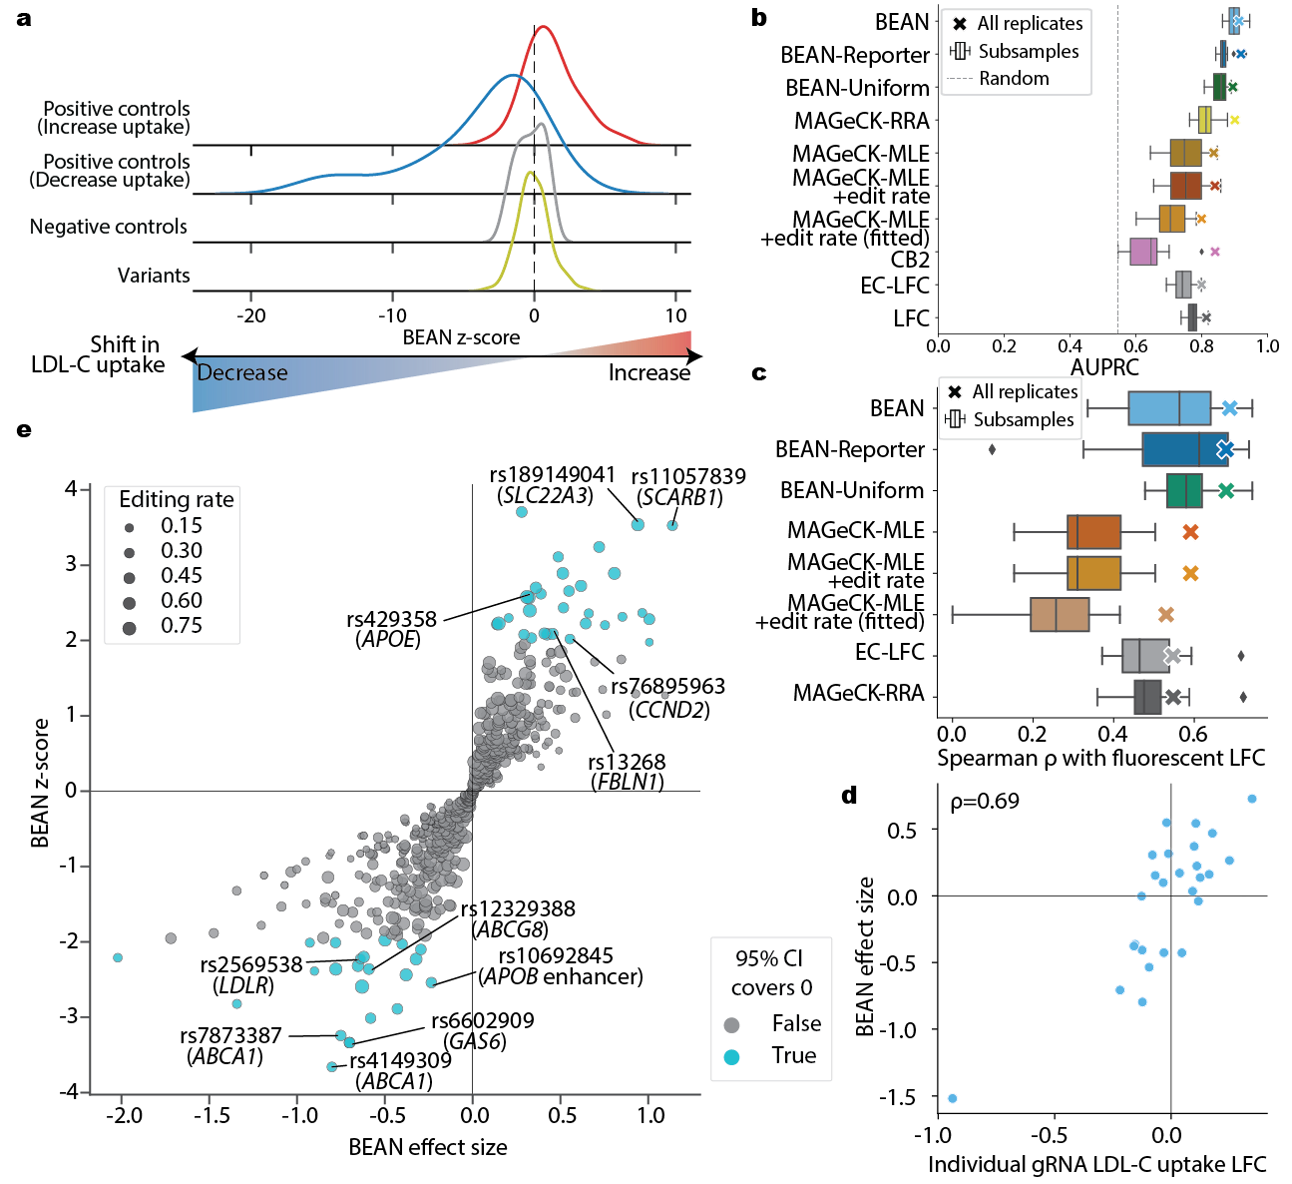
\includegraphics[width=\textwidth]{figures/crisprbean8.png}
	\caption[BEAN improves variant impact estimation from the LDL-C GWAS library screen]{\textbf{BEAN improves variant impact estimation from the LDL-C GWAS library screen.  (A)} Ridge plot of BEAN $z$-score distributions of positive controls, negative controls, and test variants. \textbf{(B)} AUPRC of classifying LDLR and MYLIP splicing variants vs.  negative controls. Metrics for all 5 replicates are shown as markers and metrics of 15 two-replicate subsamples among the 5 replicates are shown as box plots. \textbf{(C)} Spearman correlation coefficient between BEAN effect size and log fold change of LDL-C uptake following individual testing of 26 gRNAs. Metrics for all 5 replicates are shown as marker and metrics of 15 two-replicate subsamples among the 5 replicates are shown as box plots. \textbf{(D)} Scatterplot of BEAN effect size and log fold change of LDL-C uptake following individual testing of 26 gRNAs. Spearman correlation coefficient is denoted as $\rho$. \textbf{(E)} Scatterplot of variant effect size and significance estimated by BEAN. Labels show rsIDs of selected variants and dbSNP gene annotations and a manual annotation for APOB enhancer in the parenthesis.}
	\label{fig:crisprbean8}
\end{figure} 
Having demonstrated robust performance of BEAN, we evaluated our ability to characterize common variants that alter LDL-C uptake. We identified 54 variants that significantly alter LDL-C uptake (95\% CI does not contain 0). These variants include intronic variants in well-known LDL-C uptake mediators whose knockout altered LDL-C uptake in a recent genome-scale CRISPR screen37 such as ABCA1, LDLR, and SCARB1 (\textbf{Fig. \ref{fig:crisprbean8}(E)}). We additionally identified coding/intronic variants in APOE, CCND2, GAS6, and FBLN1 with strong genetic likelihood of causality (UKBB SUSIE fine-mapping PIP > 0.99 and/or the only variant in a fine-mapped credible set\citep{graham2021power}), indicating that the effect of these variants on serum LDL-C is at least partially mediated by LDL-C uptake. To validate the inferred effect sizes, we performed individual lentiviral ABE8e-SpRY transduction of HepG2 cells with gRNAs targeting 22 variants and 4 positive controls. We performed fluorescent LDL-C uptake profiling of each edited cell line mixed with an in-well control cell line in 6 biological replicates, allowing us to compare changes in LDL-C uptake with matched data from the screen. The individual LDL-C uptake log-fold-change (LFC) values showed strong correlation to the BEAN effect sizes ($\mu$, Spearman R=0.69, \textbf{Fig. \ref{fig:crisprbean8}(C)} and \textbf{D}), showing more robust correlation than BEAN-Uniform (R=0.68), log fold change based on MAGeCK-RRA (R=0.51), and regression coefficients $\beta$ of MAGeCK-MLE (R=0.61). These data demonstrate that BEAN enables accurate inference of variant effects on LDL-C uptake over a wide dynamic range.

To gain insight into a set of 20 variants for which the mechanism of LDL-C uptake alteration is less clear, we developed a pipeline to assess the cellular effects of variant installation (\textbf{Fig. \ref{fig:crisprbean9}(A)}). First, we asked which of these variants impact chromatin accessibility. We established an approach to perform pooled variant editing followed by ATAC-seq. High multiplicity of infection (MOI) lentiviral delivery of a pool of 20 ABE8e-SpRY gRNAs to HepG2 cells was followed by ATAC-seq and paired genomic DNA collection in three biological replicates in standard and serum-starved conditions. We performed multiplexed PCR enrichment of the regions surrounding each of the 20 edited variants followed by targeted amplicon sequencing by NGS. Differential representation of an alternate allele in ATAC-seq relative to gDNA sequencing implies differential accessibility of the alternate allele than the reference (\textbf{Fig. \ref{fig:crisprbean9}(B)}).
\begin{figure}
	\centering
	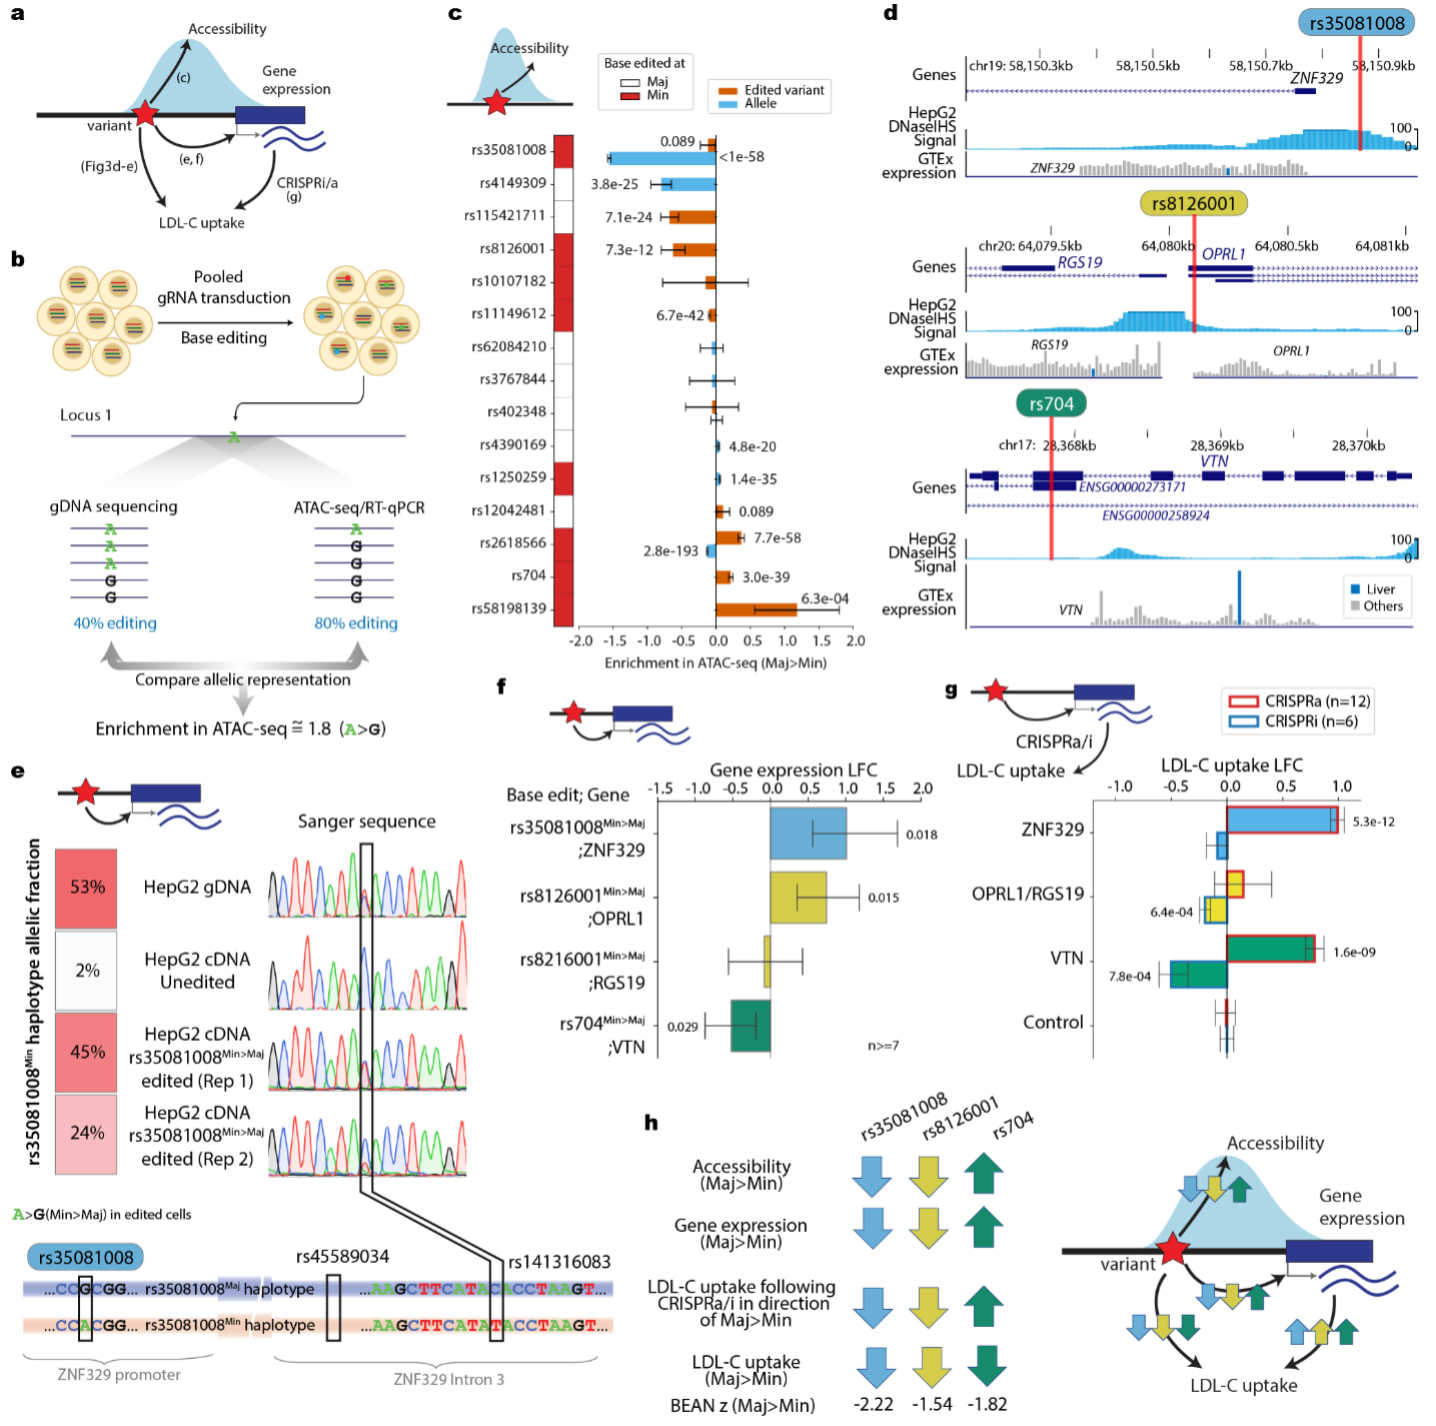
\includegraphics[width=\textwidth]{figures/crisprbean9.png}
	\caption[Functional characterization of LDL-C GWAS variants]{\textbf{Functional characterization of LDL-C GWAS variants.  (A)} Schematic of potential variant mechanisms and the figure panels showing data from each mechanistic experiment. \textbf{(B)} Schematic of pooled ATAC-seq analysis to identify variants impacting accessibility. Differential representation of allele in gDNA and ATAC-seq reflects differential accessibility induced by the base edit or heterozygous reference allele. \textbf{(C)} Change in ATAC-seq enrichment from the pooled ATAC-seq experiment. 95\% confidence intervals are shown as the error bars. “Edited variant” denotes the enrichment by base edit and “Allele” denotes the enrichment by either of the heterozygous alleles, when available, translated uniformly to major (Maj) to minor (Min) allele direction. Variants where the base edit is conducted from minor allele are denoted as red in the color bar. Family-wise error rate (FWER) with Benjamini-Hochberg multiple correction is shown for each enrichment value where FWER < 0.1. \textbf{(D)} Genomic tracks for three selected variants. DNaseIHS; DNase 1 Hypersensitivity. Multiple transcript variants of RGS19 and OPRL1 are shown in the middle panel. \textbf{(E)} Fraction of ZNF329 minor (Min) allele haplotype reads in gDNA and cDNA from untreated HepG2 and HepG2 with rs35081008Min>Maj base editing.  \textbf{(F)} Change in gene expression following base editing of three selected variants from minor (Min) to major (Maj) allele. P-values of the one sample Student’s t-test of LFC vs. mean of 0 that are smaller than 0.05 are shown above each bar. \textbf{(G)} Change in cellular LDL-C uptake following CRISPRa/i of proximal genes for three selected variants. P-values of the one sample Student’s t-test of LFC vs. mean of 0 that are smaller than 0.05 are shown above each bar. \textbf{(H)} Summary schematic of characterization results.}
	\label{fig:crisprbean9}
\end{figure} 
Eight of the 20 variants are heterozygous in HepG2, and thus we could assess whether these variants reside in chromatin accessibility quantitative trait loci (caQTL) \citep{degner2012dnase}, showing differential relative accessibility of the two haplotypes irrespective of base editing. We found five of these eight variants to be caQTLs (\textbf{Fig. \ref{fig:crisprbean9}(C)}). Two of these loci (rs35081008 and rs2618566) were also identified as caQTLs in a recent analysis of 20 human liver tissue samples \citep{currin2021genetic}. Importantly, caQTL analysis cannot address the causality of the evaluated variant due to the presence of linked variants which could contribute to the differential ATAC-seq signal. To assess whether individual variants alter chromatin accessibility, we evaluated whether base editing induces differential accessibility for any of the 20 tested variants. Technical issues including insufficient representation of the region, insufficient editing, and inability to phase heterozygous loci prevented assessment of five of the variants. Of the 15 remaining variants, eight significantly altered chromatin accessibility when edited (family-wise error rate 0.1, \textbf{Fig. \ref{fig:crisprbean9}(C)}). Four such variants (rs11149612, rs35081008, rs8126001, and rs2618566) were in loci identified as liver tissue caQTLs. Because base editing only alters a single variant in a locus, this analysis establishes at least partial causality to the tested variant. We performed deeper characterization of three variants whose editing alters both LDL-C uptake and chromatin accessibility. Rs704 is a missense coding variant in VTN and is the only variant in a fine-mapped credible set from LDL-C GWAS30, suggesting high likelihood of causality. The other two variants are in gene promoters—rs35081008 is in the ZNF329 promoter, and rs8126001 is in the shared OPRL1/RGS19 promoter \textbf{Fig. \ref{fig:crisprbean9}(D)}. Both variants have moderate probability of causality from GWAS evidence (SUSIE PIP=0.49 for rs35081008, PIP=0.25 for rs8126001), with the remaining probability in the rs35081008 locus deriving from a linked variant (rs34003091) 19-nt upstream in the ZNF329 promoter. None of the putative target genes has been previously found to alter LDL-C uptake, nor do they show significance in LDL-C burden analyses. To investigate how the prioritized variants might affect transcription factors (TF) binding sites and thereby regulate proximal genes involved in LDL-C uptake, we adapted the MotifRaptor pipeline \citep{yao2021motif}. For each variant, we retrieved genomic sequences spanning 61 bp centered around the SNP location, using the hg38 genome assembly as a reference. Each sequence was mutated by substituting the major allele with the minor allele at the SNP position, yielding both a reference and an alternative sequence for each variant. Subsequently, to evaluate the potential for transcription factor (TF) binding, we employed all the human TF position weight matrices (PWMs) from the CIS-BP database \citep{weirauch2014determination} to scan each pair of reference and alternative sequences. This motif scanning generated binding scores at each sequence position, serving as predictive indicators of TF binding potential. 
We then compared these scores for each TF across the reference and alternative alleles within every sequence pair. This comparative step is crucial for determining a variant's impact on TF binding. Specifically, higher binding scores for the alternative sequence indicate an increase in TF binding potential, while lower scores suggest a decrease. To quantify these changes, we calculated a 'disruption score' as follows: 
\[
\text{disruption} = \textrm{score($s_{alt}$)}- \textrm{score($s_{ref}$)}
\]
This score helps capture the directional change each variant induces, where a negative value signifies reduced TF binding potential and a positive value indicates an increase. For rs8126001, our approach prioritized two zinc finger TFs, ZNF333 and ZNF770 with enhanced binding site sequences due to the heterozygous minor allele in HepG2 cells (\textbf{Fig. \ref{fig:crisprbean10}}). HepG2 ChIP-seq data59 further support the binding of these TFs at this locus, although the variant lies at the edge of the peaks (\textbf{Fig. \ref{fig:crisprbean11}}). While definitive conclusions about these factors will require further experimental validation, our observations align with previous research \citep{farh2015genetic} suggesting that only a minority of causal variants directly alter canonical TF binding sequences and instead affect non-canonical sequences. 
\begin{figure}
	\centering
	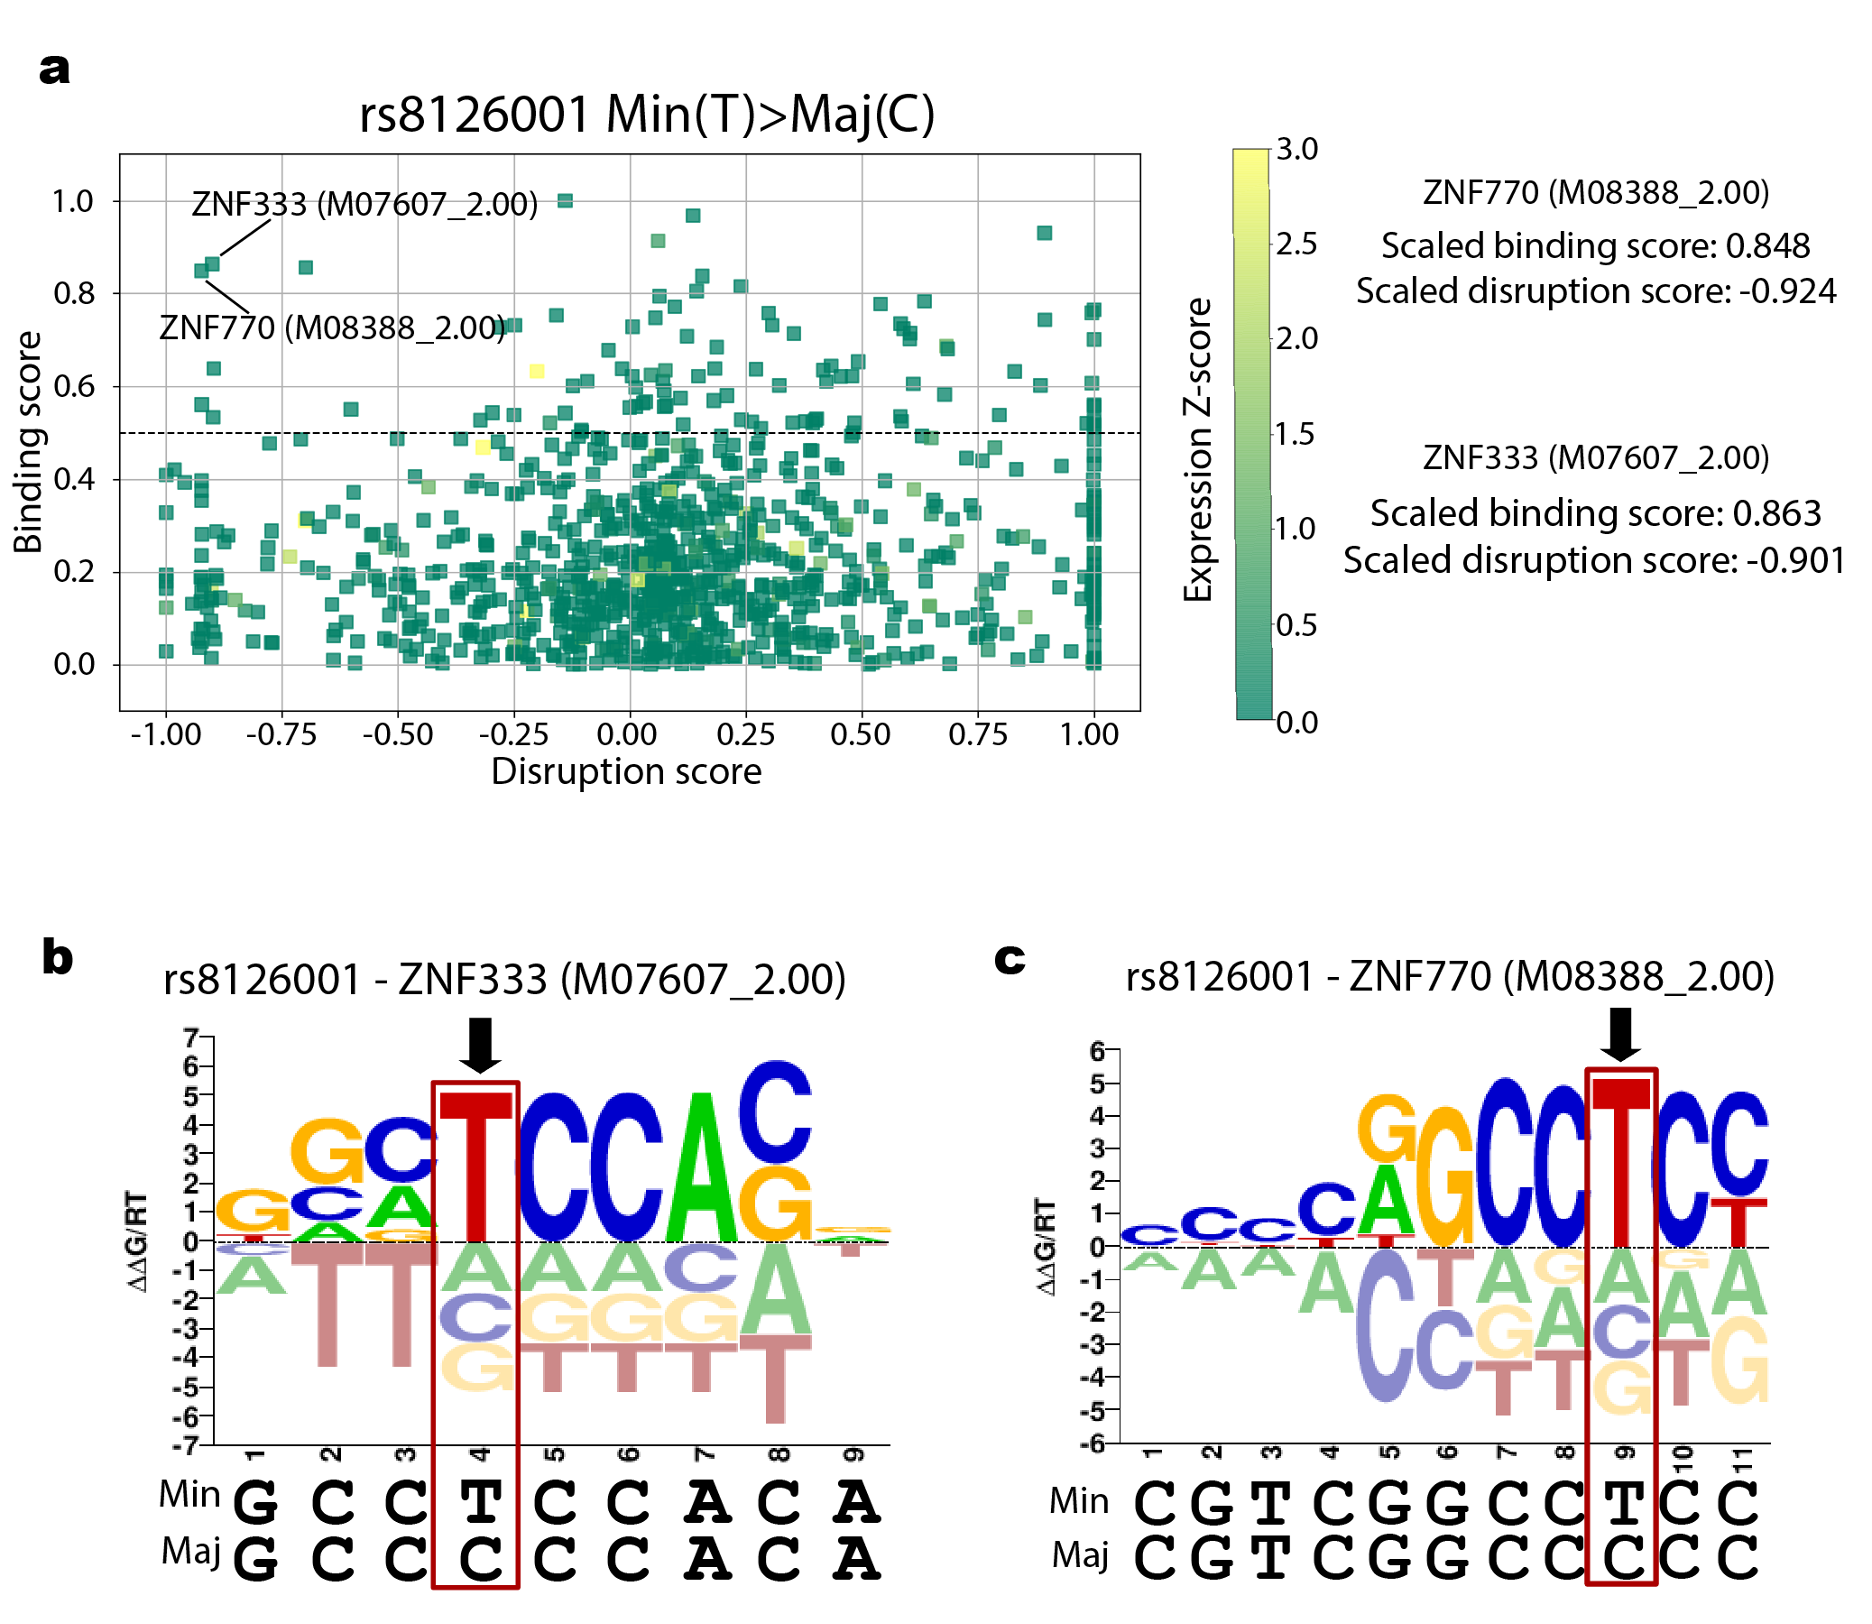
\includegraphics[width=\textwidth]{figures/crisprbean10.png}
	\caption[MotifRaptor analysis of candidate variant transcription factor binding disruption]{\textbf{MotifRaptor analysis of candidate variant transcription factor binding disruption.  (A)} Disruption plotted against binding score of motifs of rs8126001 minor allele transition to major. \textbf{(B-C)} Identified ZNF333 and ZNF770 motif aligned with rs8126001 loci with minor and major alleles.}
	\label{fig:crisprbean10}
\end{figure} 
\begin{figure}
	\centering
	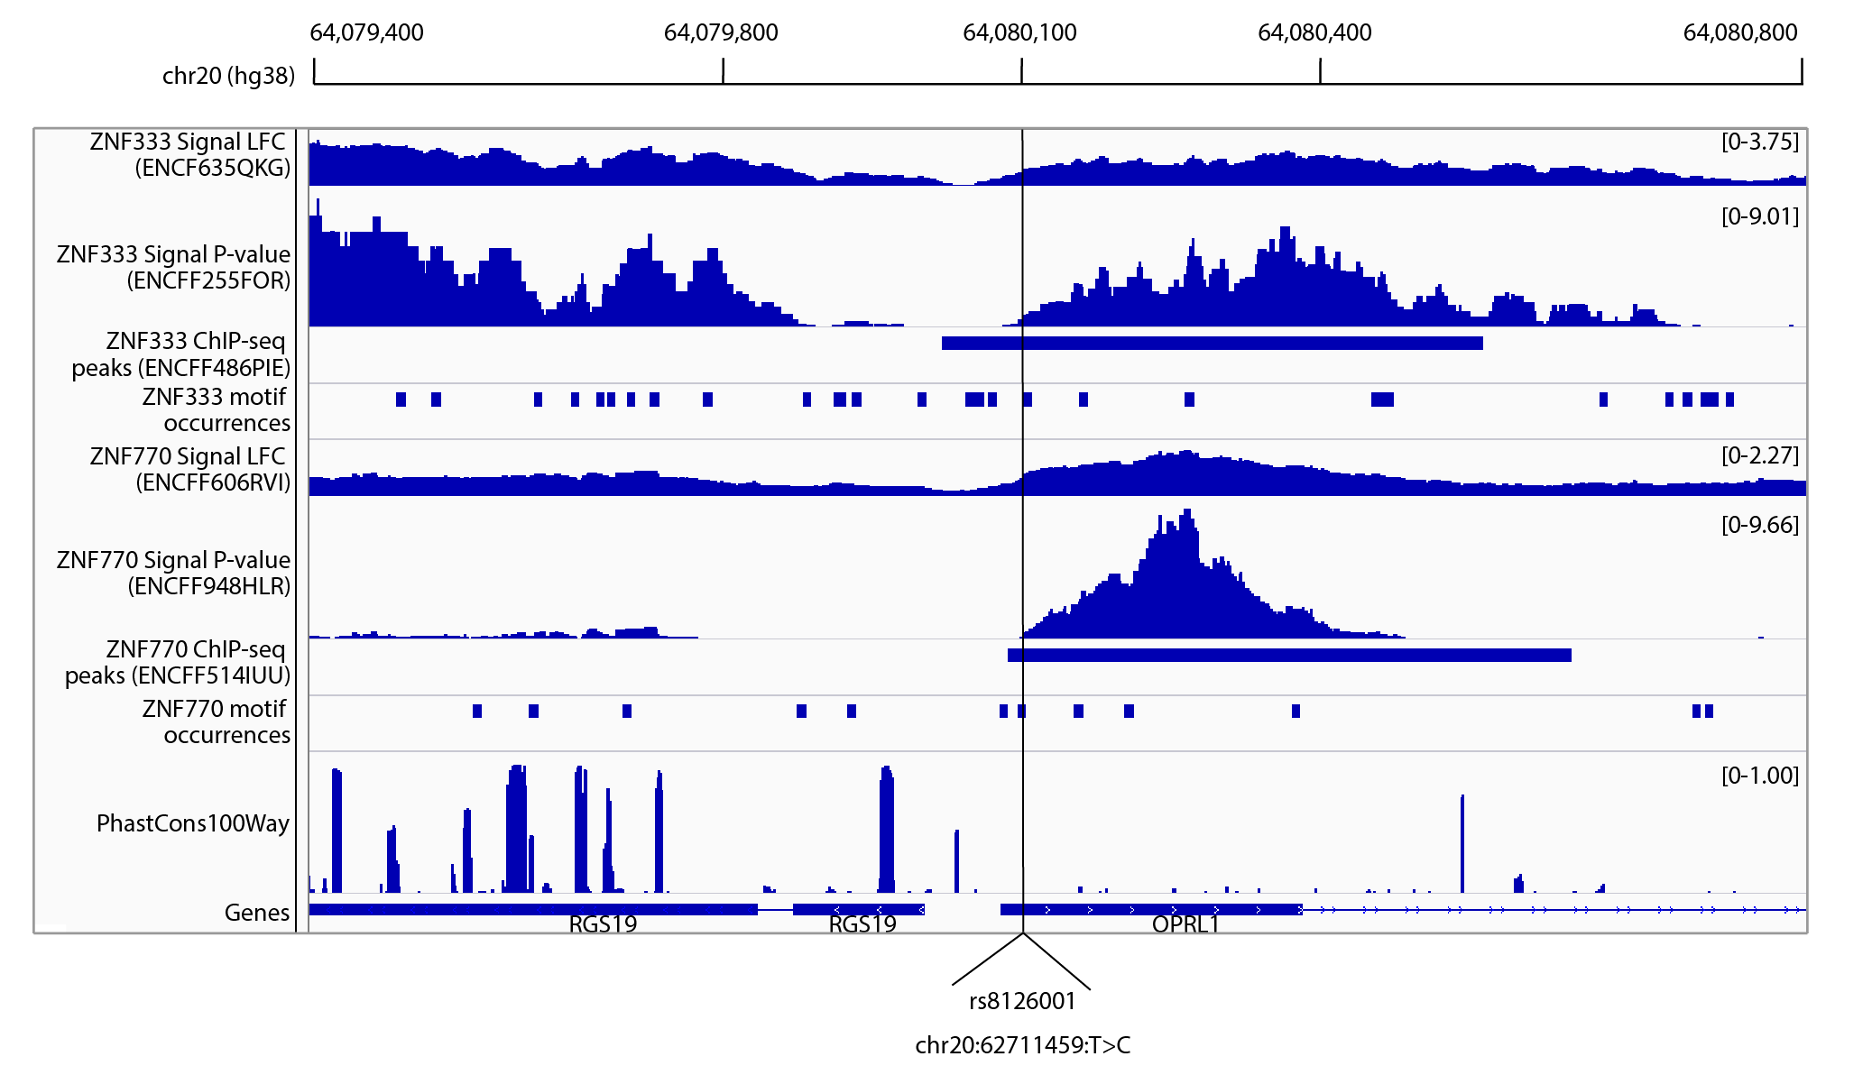
\includegraphics[width=\textwidth]{figures/crisprbean11.png}
	\caption[ChIP-seq signal LFC, signal P-values, peaks and motif occurrences of ZNF333 and ZNF770 around rs8126001]{\textbf{ChIP-seq signal LFC, signal P-values, peaks and motif occurrences of ZNF333 and ZNF770 around rs8126001.} PhastCons100way conservation scores and gene annotations are  displayed together. ENCODE accessions are shown in the parenthesis. }
	\label{fig:crisprbean11}
\end{figure} 
We confirmed through RT-qPCR analysis that editing the minor to major alleles of rs35081008 and rs8126001 leads to increased expression of ZNF329 and OPRL1 respectively (\textbf{Fig. \ref{fig:crisprbean9}(F)}), which is consistent with the increased chromatin accessibility induced by these edits. rs35081008 is heterozygous in HepG2, and we used two linked ZNF329 intronic variants to assess allele-specific expression. In wild-type HepG2, only 2\% of ZNF329 transcripts derive from the minor allele haplotype (\textbf{Fig. \ref{fig:crisprbean9}(E)}), consistent with the diminished chromatin accessibility of this allele (\textbf{Fig. \ref{fig:crisprbean9}(C)}) and the status of rs35081008 as a liver eQTL. Editing rs35081008 from minor to major allele restores expression of this haplotype to 35\% of total transcripts (\textbf{Fig. \ref{fig:crisprbean9}(E)}), providing further evidence that rs35081008Maj results in increased expression of ZNF329.We then performed CRISPRa and CRISPRi targeting to assess whether altered expression of the four candidate target genes alters LDL-C uptake. CRISPRa induction of VTN and ZNF329 significantly increased LDL-C uptake, and CRISPRi repression of VTN and OPRL1/RGS19 reduced LDL-C uptake (\textbf{Fig. \ref{fig:crisprbean9}(G)}). In our base editing experiments, rs704Min shows decreased LDL-C uptake, so we surmise that this allele must have decreased expression or function, given that decreased VTN expression decreases LDL-C uptake (\textbf{Fig. \ref{fig:crisprbean9}(H)}). Prior biochemical characterization has shown decreased cellular binding capacity of rs704Min , suggesting a possible mechanistic explanation. Our data are consistent with rs35081008Min decreasing ZNF329 expression, which in turn decreases LDL-C uptake. Finally, our data are most consistent with rs8126001Min decreasing OPRL1 expression, which leads to decreased LDL-C uptake. This observation aligns with the higher predictive binding affinity of ZNF333, a transcriptional repressor \citep{jing2004identification, witzgall1994kruppel}, with rs8126001Min and the potential disruption of its binding with rs8126001Maj. In summary, through accurately quantifying impacts of disease-associated variants on LDL-C uptake, BEAN reveals genetic mechanisms underlying control of LDL-C levels.
% -- Saturation LDLR coding sequence tiling screening enables quantitative assessment of rare variant deleteriousness 
\subsection{Saturation LDLR coding sequence tiling screening enables quantitative assessment of rare variant deleteriousness }
We next adapted BEAN to the LDLR tiling library, enhancing the model to specifically assess the contributions of individual amino acid mutations rather than SNVs, by enabling a more comprehensive understanding of coding region alterations. Previous coding sequence base editing analyses have assumed that all editable bases within a window are edited, which leads to erroneous amino acid mutation assignments, or have analyzed gRNA-level signal only \citep{martin2023massively}. We aimed to exploit the combination of dense tiling afforded by ABE8e-SpRY and reporter editing outcomes to model the effects of coding variants more accurately. The LDLR tiling screen showed high coverage of edited nucleotides and amino acids (92\% of targetable nucleotides and 74\% of the 860 LDLR amino acids in the LDLR coding sequence were edited at $>$10\% frequency by at least one gRNA in the reporter,. A total of 2,182 distinct variants were assessed, of which 874 are missense coding variants. Each gRNA produced an average of 2.6 distinct alleles, and each variant was covered by 5.8 gRNAs on average. Thus, ABE8e-SpRY tiling of LDLR resulted in a rich dataset of coding variants for the evaluation of their phenotypic impacts.
\begin{figure}
	\centering
	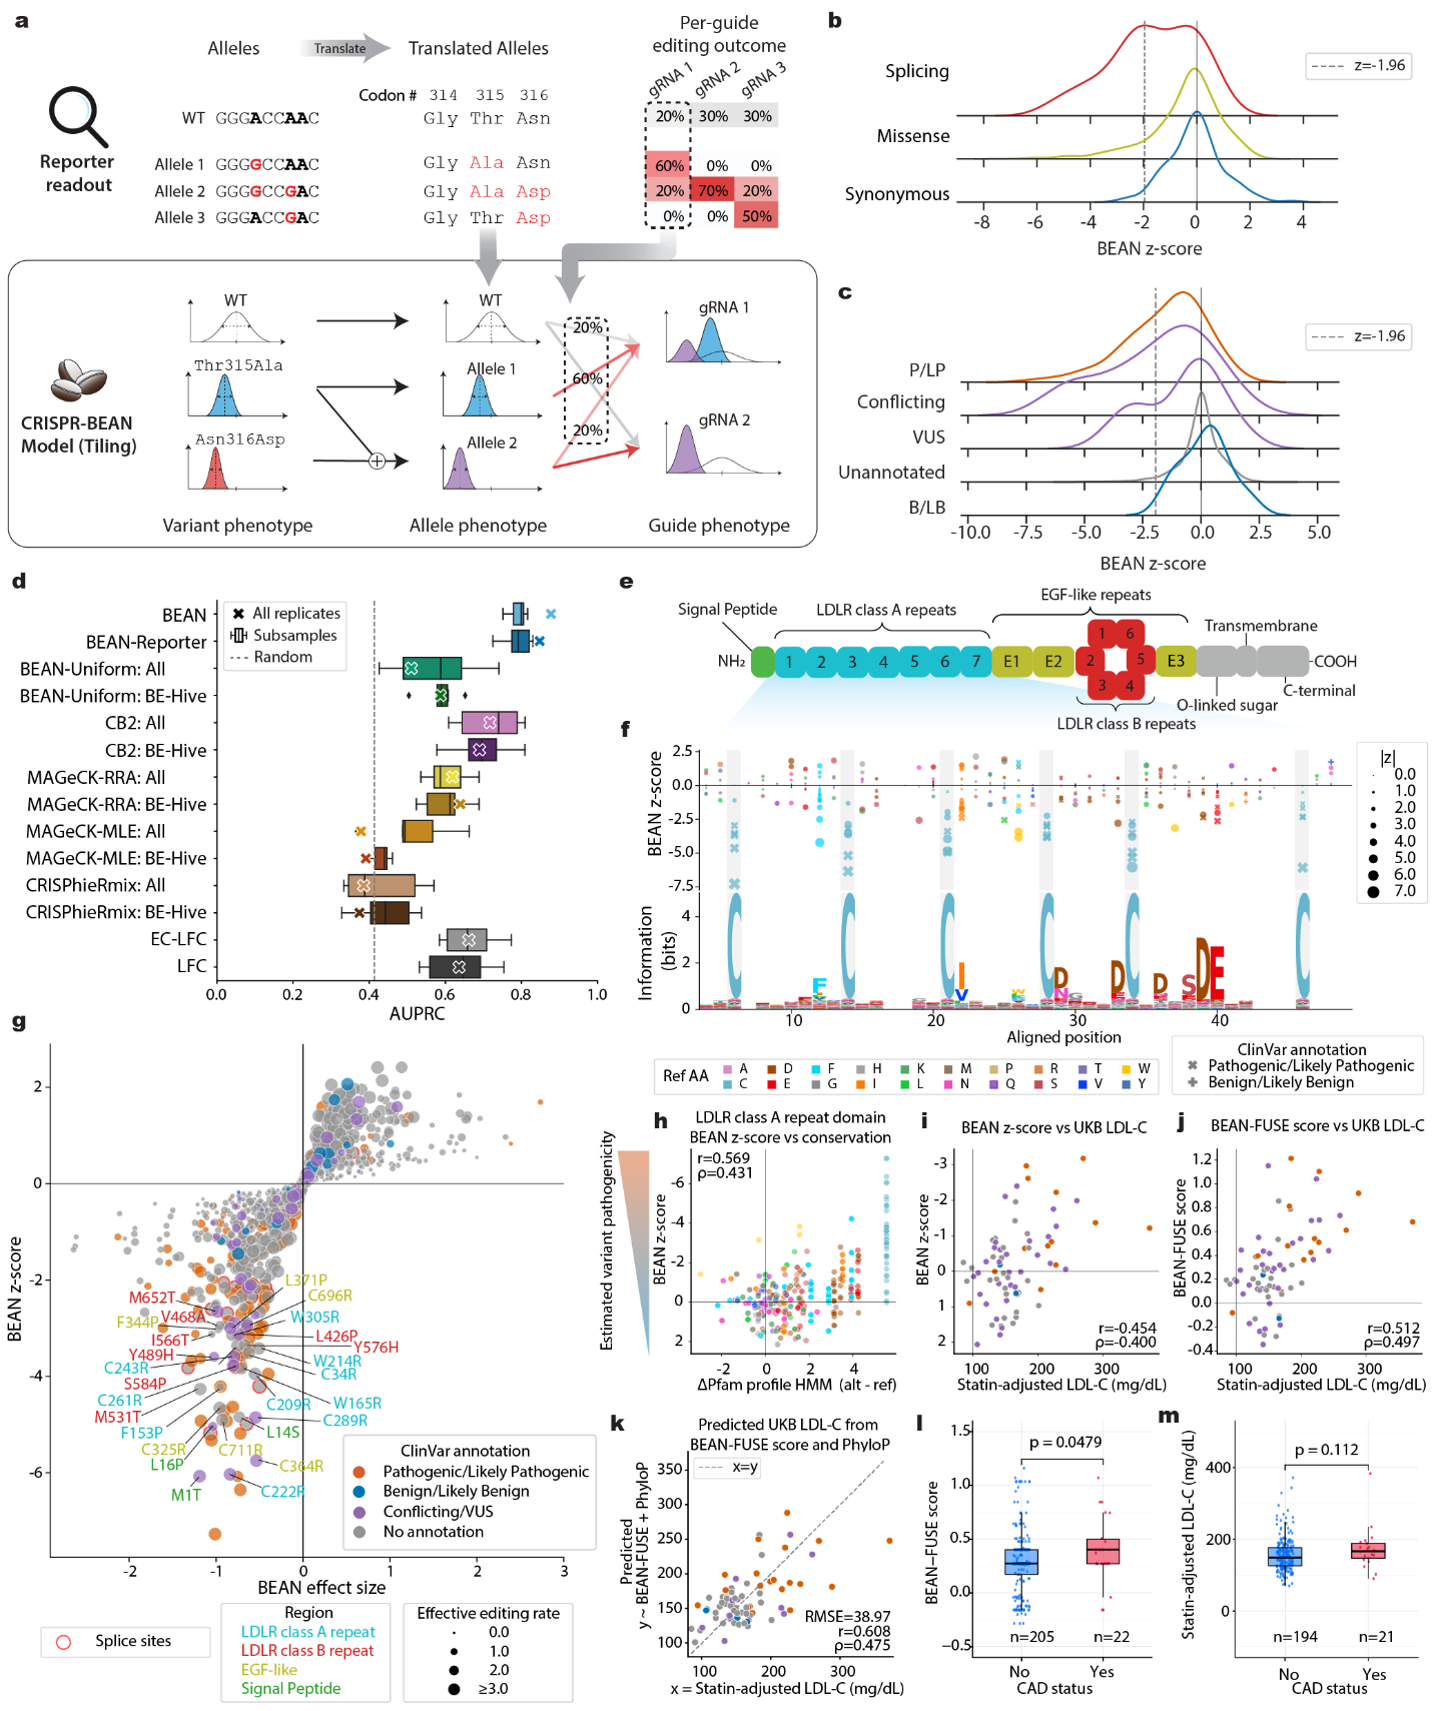
\includegraphics[width=\textwidth]{figures/crisprbean12.png}
	\caption[Dissection of LDLR variant effects through BEAN modeling of a saturation tiled base editing screen]{\textbf{Dissection of LDLR variant effects through BEAN modeling of a saturation tiled base editing screen. (A)} BEAN model for coding sequence tiling screens. Reporter editing efficiencies are calculated at the amino acid-level when the edited nucleotides are in coding region. Phenotypes of gRNAs with multi-allelic outcomes are modeled as the Gaussian mixture of allelic phenotypes. If an allele consists of more than one variant, the phenotype of the allele is modeled as the sum of the component variants. A Bayesian network is used to model variant-level phenotypes, sharing phenotypic information from all available gRNAs. \textbf{(B)} Ridge plot of BEAN z-score distributions of positive controls, negative controls, and variants. \textbf{(C)} Ridge plot of BEAN z-score distributions of Clinvar variants annotated as pathogenic/likely pathogenic (P/LP), benign/likely benign  (B/LB), conflicting interpretation of pathogenicity (conflicting), and Uncertain significance (VUS), and unannotated variants. \textbf{(D)} AUPRC of classifying ClinVar pathogenic/likely pathogenic vs. benign/likely benign variants. The marker shows the metrics of each method run on 4 replicates with no failing samples. Boxplot shows the metrics of 6 2-replicate combinations of the 4 replicates. \textbf{(E)} LDLR domain structure adopted from Oommen et al71. \textbf{(F)}BEAN $z$-scores for variants in the 7 LDLR class A repeat domains aligned with the Pfam profile HMM logo. Highly conserved cysteines are highlighted in grey. \textbf{(G)} Scatterplot of estimated variant effect sizes and z-scores. Labels of selected deleterious variants without ClinVar pathogenic/likely pathogenic annotations are shown. \textbf{(H)} Scatterplot of LDLR class A repeat missense variant BEAN $z$-scores and $\Delta$Pfam profile HMM scores. Higher $\Delta$Pfam scores correspond to substitution from highly conserved to rarely observed amino acids. \textbf{(I)} Comparison of mean statin-adjusted LDL-C level and BEAN z-score for variants observed in UKB and base editing. \textbf{(J)} Comparison of mean statin-adjusted LDL-C level and BEAN-FUSE scores for variants observed in UKB and base editing. \textbf{(K)} LDL-C levels of observed missense variants predicted by a regression model using BEAN-FUSE and PhyloP scores with 10-fold cross validation, compared with mean statin-adjusted LDL-C level in UKB. \textbf{(L)} Boxplots of BEAN-FUSE functional scores for UKB individuals with variants observed in our base editing screen with or without CAD. \textbf{(M)} Boxplots of statin-adjusted LDL-C levels of UKB invididuals with variants observed in our base editing screen with or without CAD. $P$-value of two-sided Wilcoxon rank-sum test is denoted. $r$; Pearson correlation coefficient, $\rho$; Spearman correlation coefficient}
	\label{fig:crisprbean12}
\end{figure} 
As opposed to the LDL-C GWAS analysis in which each gRNA was evaluated based on its editing frequency at a single target position, we adapted BEAN to account for multi-allelic outcomes. First, BEAN translates the edited alleles, i.e., aggregates nucleotide-level allele counts that leads to the identical amino acid transition into a single amino-acid level allele counts, while preserving nucleotide transition in non-coding regions. BEAN then filters for the translated alleles that are robustly observed for each gRNA (\textbf{Fig. \ref{fig:crisprbean12}(A)}). BEAN uses a Bayesian network to combine phenotypic information from all the gRNAs that produce a given allele. Importantly, the phenotype attributed to each gRNA is modeled as a mixture distribution of the alleles it generates, with the contribution of each allele weighted by its corresponding editing frequency.BEAN assigned significant z-scores ($<$-1.96, equivalent to 95\% credible interval not covering 0) to 145 among 2,182 variants assessed from the LDLR tiling library, 131 of which decrease LDL-C uptake. 47 variants that significantly decrease LDL-C uptake are annotated in ClinVar as pathogenic/likely pathogenic, while 17 are ClinVar VUS/conflicting variants and none are ClinVar benign/likely benign \textbf{Fig. \ref{fig:crisprbean12}(G)}), indicating that BEAN can reliably predict the pathogenicity for variants without a pathogenic or benign classification \textbf{Fig. \ref{fig:crisprbean12}(B)} and \textbf{(C)}). We compared the performance of BEAN at distinguishing ClinVar-annotated pathogenic from benign/likely benign LDLR variants to other available screen analysis methods \citep{li2014mageck, li2015quality, jeong2019beta, daley2018crisphiermix}. To allow comparison of methods that do not account for editing outcomes, we assigned outcomes to each gRNA either by assuming all editable bases within the maximal editing window are perfectly edited \citep{hanna2021massively} (“All”) or by using the most frequent predicted outcome from BE-Hive \citep{arbab2020determinants}(“BE-Hive”). As in the LDL-C GWAS screen, BEAN showed better performance than any other method \textbf{Fig. \ref{fig:crisprbean12}(D)}), and BEAN also outperformed the model variants that do not account for accessibility (BEAN-Reporter) or reporter editing outcomes (BEAN-Uniform), further justifying the modeling decision to explicitly leverage editing outcomes and accessibility. BEAN achieves an AUPRC of 0.88 at this task, indicating highly effective distinction of pathogenic and benign LDLR variants through scoring HepG2 LDL-C uptake proficiency. To gain insight into mechanisms by which these variants disrupt LDL-C uptake, we examined BEAN z-scores for variants that reside within conserved functional domains \textbf{Fig. \ref{fig:crisprbean12}(E)} and \textbf{(F)}). LDLR contains seven highly conserved LDLR class A repeats that bind to LDL. The LDLR class A repeat is structurally anchored by six highly conserved cysteines that form three disulfide bonds \citep{fass1997molecular}. As expected, many of the missense variants with the strongest effects on LDLR function disrupt these cysteines \textbf{Fig. \ref{fig:crisprbean12}(F)}). We find that cysteine mutating edits in each of the seven LDLR class A repeats disrupt LDLR activity, suggesting that structural integrity of all repeats is required for efficient LDL binding, although disruption is most impactful in repeats 3-7. Truncation experiments have reported that repeats 1 and 2 are dispensable for LDL binding \citep{russell1989different} in partial accord with our results \citep{jeon2005structure}. To examine the relationship between conservation and function more comprehensively in these repeats, we compared the BEAN $z$-score of every installed variant with its change in amino acid conservation score from the Pfam profile HMM66. We observed strong concordance (Pearson r = 0.57 \textbf{Fig. \ref{fig:crisprbean12}(H)}), with N-terminal hydrophobic residues and C-terminal calcium-coordinating acidic residues within the repeats also showing particular functional importance, as expected from the known function of these domains.Encouraged by the concordance between our screen and conservation scores within the LDLR class A repeats, we asked whether BEAN scores could predict functional impairment across the entire LDLR gene. We examined statin-adjusted LDL-C levels \citep{global2013discovery} in the UK Biobank (UKB) for individuals with paired exome sequencing and lipid level data. To control for the contribution of other variants in genes known to impact serum LDL-C level, we filtered out individuals who harbor nonsynonymous APOB or PCSK9 variants or multiple LDLR missense variants, leading to 9,819 individuals harboring 358 distinct LDLR missense variants. There are 76 distinct LDLR missense variants observed in our base editing data with UKB carriers. We observe robust concordance between the average carrier LDL-C and BEAN scores for these variants (Spearman $\rho$ = 0.40, Pearson r = 0.45, \textbf{Fig. \ref{fig:crisprbean12}(I)}, suggesting that BEAN provides accurate quantitative prediction of the impact of LDLR missense variants on control of serum LDL-C levels in the human population. As our base editing screen does not exhaust possible mutation types per position, we used the FUSE \citep{yu2023joint} pipeline to impute the impact of unobserved variants at positions at which a different missense variant is scored. FUSE uses an amino acid substitution matrix derived from 24 deep mutational scanning datasets to impute functional scores for all possible missense variants at positions observed in base editing data (BEAN+FUSE score, see Methods). Applying FUSE to the 76 UKB variants with observed base editing data, BEAN-FUSE shows improved correlation with UKB carrier LDL-C (Spearman $\rho$ = 0.50, Pearson r = 0.51, \textbf{Fig. \ref{fig:crisprbean12}(J)}). BEAN-FUSE correlation with UKB carrier LDL-C was robust but lower at all 358 missense LDLR variants with lipid measurements (Spearman $\rho$ = 0.37, Pearson r = 0.35). Altogether, BEAN-FUSE provides a pipeline to extend base editing screening to predict functional impairment for unobserved missense variants, although our data suggest that accuracy does decrease for unobserved variants. As base editing provides orthogonal functional assessment to conservation, we asked whether the LDL-C levels of UKB variant carriers could be predicted with BEAN-FUSE scores and PhyloP 100way vertebrate conservation scores. Using XGBoost regression \citep{chen2016xgboost}, we achieved more robust correlation with UKB carrier LDL-C than either BEAN-FUSE or PhyloP alone at the 76 variants observed in the base editing screen (Spearman $\rho$ = 0.48, Pearson r = 0.61, RMSE=39.0, \textbf{Fig. \ref{fig:crisprbean12}(K)}) and at 358 variants with BEAN-FUSE score (Spearman $\rho$ = 0.37, Pearson r = 0.31, RMSE=51.1). This result demonstrates the potential utility of base editing data to improve quantitative phenotype prediction combined with computational prediction methods. Individuals with pathogenic FH variants are at higher risk of coronary artery disease (CAD), even after controlling for LDL-C levels \citep{clarke2022coronary}. However, the vast majority of rare LDLR missense variants lack ClinVar pathogenic/likely pathogenic designations, preventing information about these potentially disease-causing variants from being shared with patients. Therefore, we asked whether CAD incidence within LDLR variant carriers could be stratified by functional scores. We found that for individuals with rare LDLR variants, functional scores processed by BEAN-FUSE were significantly higher for patients with prevalent or incident CAD (Wilcoxon rank-sum test, p = 0.0479, \textbf{Fig. \ref{fig:crisprbean12}(L)}). BEAN-FUSE scores provided more robust stratification of individuals with CAD than statin-adjusted LDL-C values for individuals with variants covered in the screen (Wilcoxon rank-sum test, p = 0.112, \textbf{Fig. \ref{fig:crisprbean12}(M)}). This demonstrates the advantage of quantifying genetic risk, which has a lifelong impact on LDL-C levels, over the snapshot provided by a single LDL-C measurement. Overall, we show that activity-normalized base editing screening can yield accurate quantitative estimation of LDLR variant pathogenicity in a large human cohort.
% -- Structural basis of LDLR missense variants 
\subsection{Structural basis of LDLR missense variants }
We further analyzed LDLR missense variants identified to significantly impair LDL-C uptake by BEAN to gain insight into mechanisms of their pathogenicity. We first examined variants with top $z$-scores that are unannotated or annotated as conflicting, or VUS in ClinVar. The top ranked variant, which shows even more significant loss-of-function than splice-ablating variants, alters the start codon, preventing full-length LDLR translation. Other top variants such as C222R, C261R, C289R, and C364R disrupt conserved disulfide bond-forming cysteines in LDLR class A repeats and EGF-like domains. Top-ranked variant in the of the signal peptide L16P  substitute hydrophobic leucines with prolines in the transmembrane alpha helix, which is likely to distort the alpha helix \citep{kim1999positional} and the  neighboring L15P has been shown to reduce LDLR transport to the plasma membrane \citep{pavlouvskova2016functional} Neighboring L14S that also ranks high substitutes hydrophobic leucine with serine in the hydrophobic h-region central to the signal peptide \citep{von1985signal}. Additionally, multiple variants disrupt calcium ion binding, which is key to LDLR class A repeat folding \citep{pena2010calcium} through the conversion of negatively charged amino acids (D/E) to glycine (G), thereby disrupting ionic interactions with side-chain carboxylates and calcium ions (D94G, E101G, E179G, D307G) in LDLR class A repeats. We also found that L371P, a VUS, disrupts a calcium ion interaction in the EGF-like domain by breaking the coordinate covalent bond between the calcium ion and the carbonyl group within the L371 main chain due to backbone distortion. Finally, we found that F153P significantly interfered with hydrophobic interactions between the aromatic ring and the attached saccharide on Q182.
\begin{figure}
	\centering
	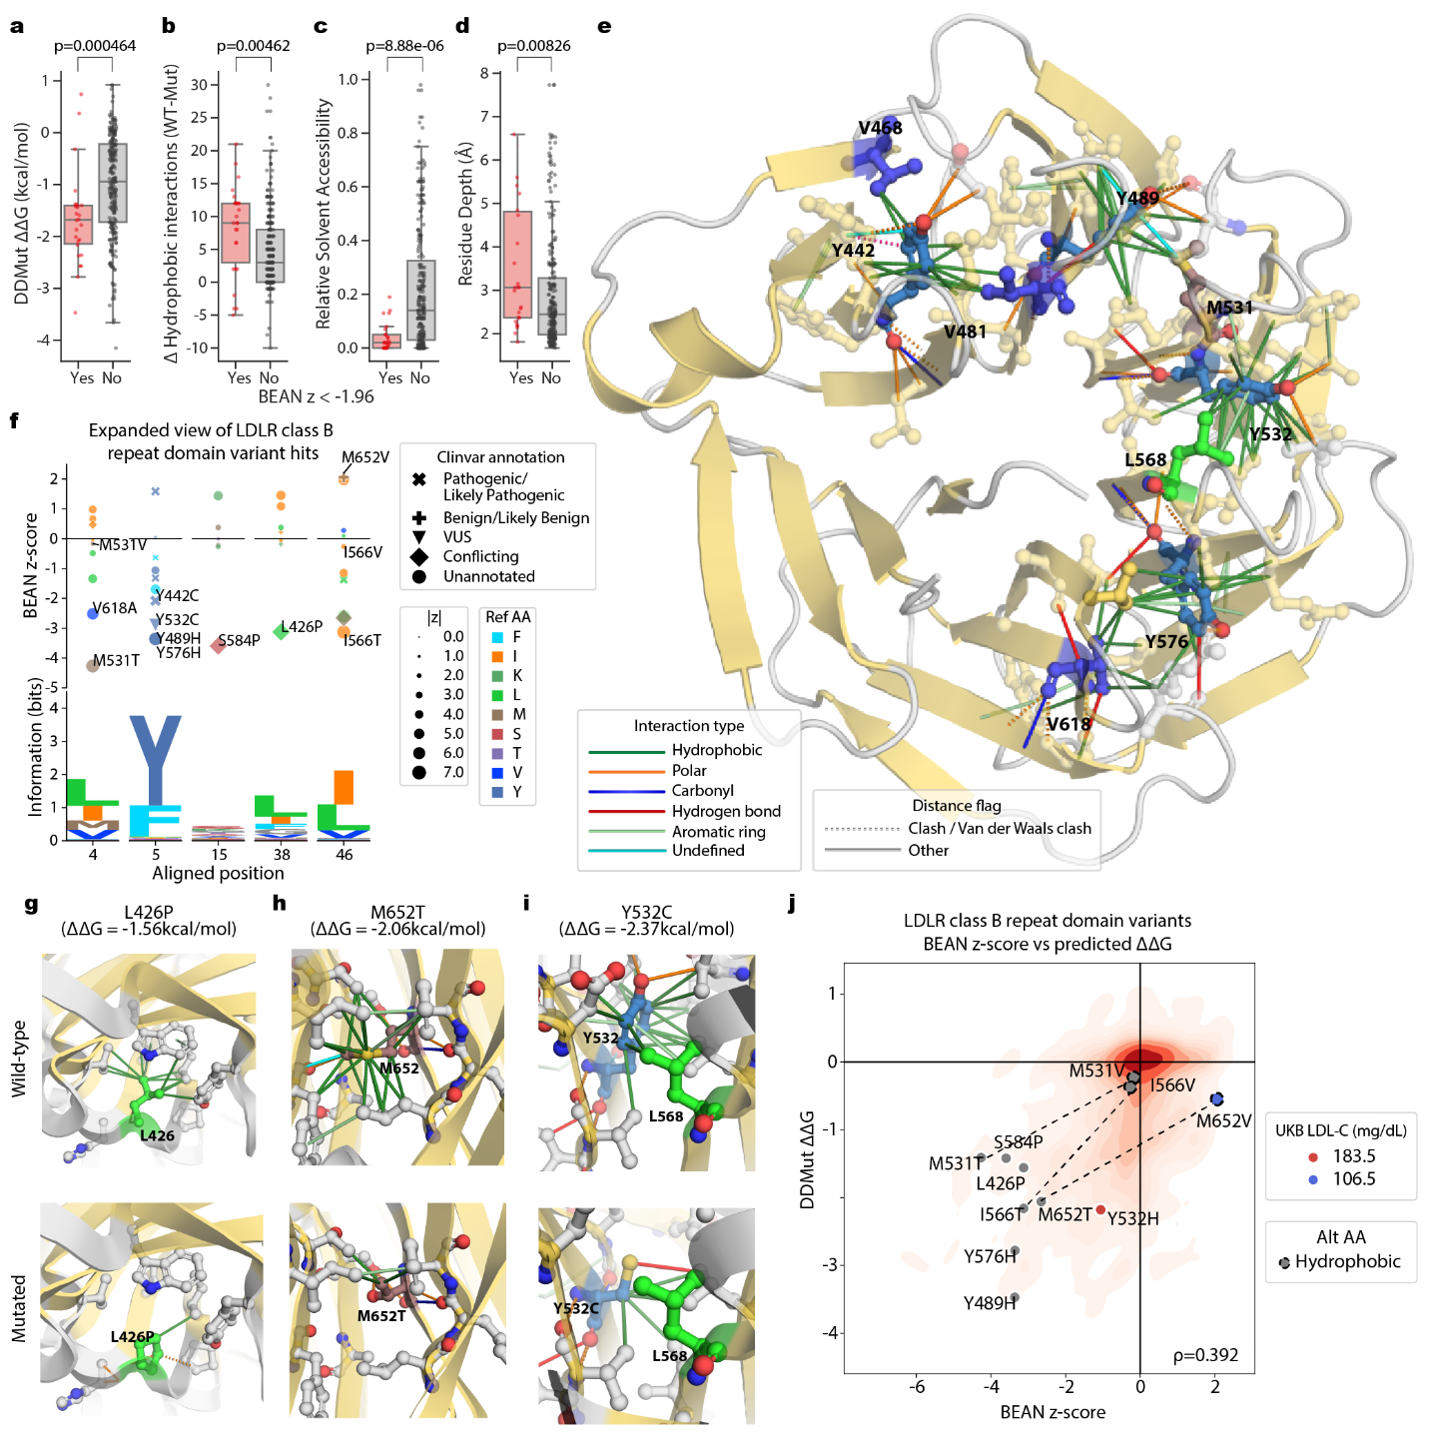
\includegraphics[width=\textwidth]{figures/crisprbean13.png}
	\caption[Deleterious variants in LDLR class B repeats weaken hydrophobic interactions]{\textbf{Deleterious variants in LDLR class B repeats weaken hydrophobic interactions (A)-(D)} Boxplots of 26 significant ($z$ < -1.96) and the rest of 259 variants observed in LDLR class B repeats. $P$-values of two-sided Wilcoxon rank-sum test are denoted. WT; wild-type, Mut; mutated. \textbf{(E)} Conserved interactions involving tyrosine of which mutation showed significant BEAN scores. Simplified interaction types and distance flags as annotated by Arpeggio are shown in the legend. \textbf{(E)} BEAN $z$-scores of positions with conserved hydrophobic residues are shown along with the LDLR class B repeat PFAM HMM logo. \textbf{(G)-(I)} Local atomic interaction in wild-type and mutated structure for ClinVar conflicting variants or VUS L426P, M652T, and Y532C. Residues in the variant positions are colored by the reference amino acids. Residues that interact with the variant position are shown. Variant position and interacting residues are colored by elements (O: red, N: blue, S: yellow). \textbf{(J)} Contour plot of BEAN z-score against $\Delta\Delta$G predicted by DDMut for 872 missense variants. Positions with distinct observed missense variants that disrupt and conserve hydrophobic sidechains are connected by dashed line.}
	\label{fig:crisprbean13}
\end{figure} 
We noticed that an appreciable number of deleterious variants that lack ClinVar pathogenic designation reside in the six LDLR class B repeats. The LDLR class B repeats, also known as YWTD repeats, form a propeller-like structure involved in the release of LDL following its endocytosis. To gain insights into unannotated variant impact, focusing on the LDLR class B repeats, we used the full wild-type LDLR structure from the AlphaFold Protein Structure Database \citep{jumper2021highly, varadi2022alphafold} and the MODELLER \citep{webb2016comparative} -generated mutant structures to calculate changes in interatomic interactions using Arpeggio \citep{jubb2017arpeggio}. Additionally, we predicted the effects of variants on protein stability ($\Delta\Delta$G, negative value indicates destabilization) with DDMut \citep{zhou2023ddmut}. We found that the 26 significant LDLR class B variants induce more destabilizing effects, disrupt more hydrophobic interactions, have lower relative solvent accessibility \citep{rose1985hydrophobicity} (0.041 of maximum residue solvent accessibility), and have higher wild-type residue depth as compared to the other observed variants in this region (\textbf{Fig. \ref{fig:crisprbean13}(A)-(D)}). Collectively, these observations strongly indicate that these significant LDLR class B repeat variants are predominantly buried within the protein core where they engage in extensive hydrophobic interactions essential for protein folding. Moreover, we found a conserved interaction across repeat domains in which a tyrosine holds neighboring propeller blades together through interactions with a hydrophobic residue of the neighboring repeat (\textbf{Fig. \ref{fig:crisprbean13}(E)-(F)}. 

We identified five of these variant pairs (Y442C with V481A, Y442C with V468A, Y489H with M531T, Y532C with L568P, and Y576H with V618A), where all nine positions have at least one variant that weakens their hydrophobic interaction and has a significant BEAN $z$-score. Among the top-ranked unannotated or ClinVar VUS and conflicting variants within LDLR class B repeats, the six most significant variants (L426P, Y489H, M531T, I566T, S584P, and Y576H) all disrupt residues that hold the propeller blades together through hydrophobic interactions (\textbf{Fig. \ref{fig:crisprbean13}(G)-(I)}). Further supporting the importance of hydrophobic interactions, the base editing screen installed additional missense variants at positions 531, 566, and 652 that conserve hydrophobicity. In all cases, mutation into hydrophobic residues has less severe impact from the base editing screen and DDMut-predicted destabilization than mutation into non-hydrophobic residues (\textbf{Fig. \ref{fig:crisprbean13}(J)}). For example, while we find M652T to be highly deleterious (BEAN $z$=-2.65), we find no functional disruption from the hydrophobicity-conserving M652V variant (BEAN $z$=+2.06). This analysis is supported clinically, as M652V is designated in ClinVar as “Likely Benign,” and the average UKB carrier LDL-C is below average (106mg/dL). In summary, structural analysis of rare LDLR variants identified by BEAN provides a basis for the missense variant impact through affecting structural integrity of LDLR, highlighting a central role for hydrophobic interactions that hold together adjacent beta blades of the LDLR class B repeat domain
% ------  begin bibliography
\bibliography{biblio}
\bibliographystyle{natbib}





\end{document}